\documentclass[10pt,a4paper]{article}
\usepackage{enumerate}
\usepackage{courier}
\usepackage{graphicx}
% \usepackage{tabularx}
% \usepackage{longtable}
%^ using xltabular instead as it includes the capabilities of both of the above
\usepackage{xltabular}
\usepackage[export]{adjustbox}
\usepackage{float}
\usepackage[utf8]{inputenc}
\usepackage[english]{babel}
\usepackage[english]{isodate}
\usepackage[parfill]{parskip}
\usepackage[margin=1.1in]{geometry}
\usepackage[titletoc,title]{appendix}
\usepackage{caption}
\usepackage{listings}
\usepackage{url}
\usepackage{pbox}
\usepackage{makecell}
\usepackage[T1]{fontenc}

\captionsetup{justification=raggedright, singlelinecheck=false}

% Fix for weird errors when quotes are in a string
\let\textquotedbl=" 

\newenvironment{spaceditemize}
{ \begin{itemize}
    \setlength{\itemsep}{5pt}
    \setlength{\parskip}{0pt}
    \setlength{\parsep}{0pt}     }
{ \end{itemize}                  } 

\newenvironment{spacedenumerate}
{ \begin{enumerate}
    \setlength{\itemsep}{5pt}
    \setlength{\parskip}{0pt}
    \setlength{\parsep}{0pt}     }
{ \end{enumerate}                } 

%%%%%%%%%%%%%%%%%%%%%%%%
% Commandline stuff
%%%%%%%%%%%%%%%%%%%%%%%
\usepackage{color}

\lstset{frame=leftline,
  aboveskip=3mm,
  belowskip=3mm,
  showstringspaces=false,
  columns=flexible,
  basicstyle={\small\ttfamily},
  numbers=none,
  breaklines=true,
  breakatwhitespace=true,
  tabsize=2
}

%%%%%%%%%%%%%%%%%%%%%%%%
% YAML stuff
%%%%%%%%%%%%%%%%%%%%%%%%
\usepackage[dvipsnames]{xcolor}

\newcommand\YAMLcolonstyle{\color{black}\mdseries\small}
\newcommand\YAMLkeystyle{\color{black}\bfseries\ttfamily\small}
\newcommand\YAMLvaluestyle{\color{black}\mdseries\small}

\makeatletter

% here is a macro expanding to the name of the language
% (handy if you decide to change it further down the road)
\newcommand\language@yaml{yaml}

\expandafter\expandafter\expandafter\lstdefinelanguage
\expandafter{\language@yaml}
{
  keywords={true,false,null,y,n},
  keywordstyle=\color{black}\bfseries\ttfamily,
  basicstyle=\YAMLkeystyle,                                 % assuming a key comes first
  sensitive=false,
  comment=[l]{\#},
  morecomment=[s]{/*}{*/},
  commentstyle=\ttfamily\mdseries\textit,
  stringstyle=\YAMLvaluestyle\ttfamily,
  moredelim=[l]{\&},
  moredelim=[l]{*},
  moredelim=**[il][\YAMLcolonstyle{:}\YAMLvaluestyle]{:},   % switch to value style at :
  morestring=[b]',
  morestring=[b]",
  literate =    %{---}{{\ProcessThreeDashes}}3
                {>}{{\textgreater}}1     
                {|}{{\textbar}}1 
                {\ -\ }{{\mdseries\ -\ }}3,
}

% switch to key style at EOL
\lst@AddToHook{EveryLine}{\ifx\lst@language\language@yaml\YAMLkeystyle\fi}
\makeatother

%\newcommand\ProcessThreeDashes{\llap{\color{black}\mdseries-{-}-}}
%%%%%%%%%%%%%%%%%%%%%%%%
%%%%%%%%%%%%%%%%%%%%%%%%
\usepackage{minted}

% Solarized color definitions
\definecolor{sbase03}{HTML}{002B36}
\definecolor{sbase02}{HTML}{073642}
\definecolor{sbase01}{HTML}{586E75}
\definecolor{sbase00}{HTML}{657B83}
\definecolor{sbase0}{HTML}{839496}
\definecolor{sbase1}{HTML}{93A1A1}
\definecolor{sbase2}{HTML}{EEE8D5}
%\definecolor{sbase3}{HTML}{FDF6E3}
% changing this a bit for readability in pdf
\definecolor{sbase3}{HTML}{FEF9ED}
\definecolor{syellow}{HTML}{B58900}
\definecolor{sorange}{HTML}{CB4B16}
\definecolor{sred}{HTML}{DC322F}
\definecolor{smagenta}{HTML}{D33682}
\definecolor{sviolet}{HTML}{6C71C4}
\definecolor{sblue}{HTML}{268BD2}
\definecolor{lblue}{HTML}{0085ff}
\definecolor{scyan}{HTML}{2AA198}
\definecolor{sgreen}{HTML}{859900}
\definecolor{darkblue}{HTML}{0000A0}
\definecolor{white}{HTML}{ffffff}

% Solarized CStyle definition
\lstdefinestyle{CStyle}{
basicstyle=\color{sbase01}\ttfamily,
backgroundcolor=\color{sbase3},
keywordstyle=\color{lblue},%scyan
commentstyle=\color{sbase1},
stringstyle=\color{sorange},
identifierstyle=\color{syellow},%sbase00
numberstyle=\color{sbase00},
% Break long lines into multiple lines?
breaklines=true,
sensitive=true,
% Show a character for spaces?
showstringspaces=false,
% 
breakatwhitespace=false,         
captionpos=b,                    
keepspaces=true,                 
numbers=left,                    
numbersep=5pt,                  
showspaces=false,                
% showstringspaces=false,
% showtabs=false,                  
tabsize=2,
language=C
}

\newminted{C}{
    %style=solarized-light,
    bgcolor=sbase3,
    autogobble=true,
    breaklines=true,
    breakanywhere,
    fontsize=\small,
    linenos
}

\newmintedfile[ccodef]{C}
{
    %style=solarized-light,
    bgcolor=sbase3,
    autogobble=true,
    breaklines=true,
    breakanywhere,
    fontsize=\small,
    linenos
}

\newminted{cpp}{
    %style=solarized-light,
    bgcolor=sbase3,
    autogobble=true,
    breaklines=true,
    breakanywhere,
    linenos
}

\newmintedfile[cppcodef]{cpp}
{
    %style=solarized-light,
    bgcolor=sbase3,
    autogobble=true,
    breaklines=true,
    breakanywhere,
    linenos
}

\newminted{ada}{
    style=solarized-light,
    bgcolor=sbase3,
    fontsize=\small,
    autogobble=true,
    breaklines=true,
    breakanywhere,
    linenos
}

\newmintedfile[adacodef]{ada}
{
    style=solarized-light,
    bgcolor=sbase3,
    fontsize=\small,
    autogobble=true,
    breaklines=true,
    breakanywhere,
    linenos
}

\newminted{yaml}{
    style=solarized-light,
    bgcolor=sbase3,
    fontsize=\small,
    autogobble=true,
    breaklines=true,
    breakanywhere,
    linenos
}

\newmintedfile[yamlcodef]{yaml}
{
    style=solarized-light,
    bgcolor=sbase3,
    fontsize=\small,
    autogobble=true,
    breaklines=true,
    breakanywhere,
    linenos
}

\newminted{python}{
    style=solarized-light,
    bgcolor=sbase3,
    fontsize=\small,
    autogobble=true,
    breaklines=true,
    breakanywhere,
    linenos
}

\newmintedfile[pythoncodef]{python}
{
    style=solarized-light,
    bgcolor=sbase3,
    fontsize=\small,
    autogobble=true,
    breaklines=true,
    breakanywhere,
    linenos
}

\newminted{matlab}{
    style=solarized-light,
    bgcolor=sbase3,
    fontsize=\small,
    autogobble=true,
    breaklines=true,
    breakanywhere,
    linenos
}

\newmintedfile[matlabcodef]{matlab}
{
    style=solarized-light,
    bgcolor=sbase3,
    fontsize=\small,
    autogobble=true,
    breaklines=true,
    breakanywhere,
    linenos
}

\newminted{latex}{
    style=solarized-light,
    bgcolor=sbase3,
    fontsize=\small,
    autogobble=true,
    breaklines=true,
    breakanywhere,
    linenos
}

\newmintedfile[latexcodef]{latex}
{
    style=solarized-light,
    bgcolor=sbase3,
    fontsize=\small,
    autogobble=true,
    breaklines=true,
    breakanywhere,
    linenos
}

\newminted{text}{
    style=solarized-light,
    bgcolor=sbase3,
    fontsize=\small,
    autogobble=true,
    breaklines=true,
    breakanywhere,
    linenos
}

\newmintedfile[textcodef]{text}
{
    style=solarized-light,
    bgcolor=sbase3,
    fontsize=\small,
    autogobble=true,
    breaklines=true,
    breakanywhere,
    linenos
}

\lstdefinestyle{pcode}{
  basicstyle=\ttfamily,
  keywordstyle=\color{darkblue},
  keywords={if,import,qualified,as,do,where,and,then,end,else,is}
}



\usepackage[colorlinks = true,
            linkcolor = black,
            urlcolor  = black,
            citecolor = black,
            anchorcolor = black]{hyperref}
\usepackage[titletoc]{appendix}

\usepackage{setspace}
\usepackage{etoolbox}
\usepackage{wrapfig}
\AtBeginEnvironment{quote}{\singlespacing\small}
\AtEndEnvironment{quote}{\vspace{-\topsep}\endsinglespace}

\makeatletter
\newcommand\HUGE{\@setfontsize\Huge{38}{47}}
\makeatother 

\begin{document}

\title{
\begin{figure}[H]
  
\includegraphics[width=0.8\textwidth,center]{../logos/adamant_logo_text_black.png}
\end{figure}
\vspace{-10mm}
\Huge{User Guide} \\
%% \large\textit{Adamant Software Framework}
\vspace{110mm}
\begin{figure}[H]
  
\includegraphics[width=0.46\textwidth,center]{images/lasp.png}
\end{figure}
\vspace{3mm} %5mm vertical space
\small{Created at:} \\
\small{Laboratory for Atmospheric and Space Physics} \\
\small{University of Colorado}  \\
\small{Boulder, Colorado} \\
}
\author{}

\date{}
\maketitle
\thispagestyle{empty}
\newpage

\pagenumbering{roman}
\tableofcontents

\newpage
\pagenumbering{arabic}
\section{About this Guide}

\subsection{Purpose}

Adamant is a component-based, model-driven framework designed to construct reliable and reusable embedded, real-time software systems. The purpose of this document is to discuss how to use the Adamant framework to design and implement a software system for a particular project. The intended audience of this document is embedded software engineers who want to understand how to use Adamant to develop their systems. It is expected that readers of this document have already read the \href{https://github.com/lasp/adamant/blob/main/doc/architecture_description_document/architecture_description_document.pdf}{\textcolor{blue}{Architectural Description Document}} for Adamant to ensure understanding of the architectural principles which govern the framework. This User Guide expands on the Architectural Description Document by providing details of how the architecture is implemented and most importantly, how it can be used. This document also assumes reader knowledge of object-oriented design and its common patterns. A cursory understanding of Ada, the implementation language of the Adamant framework, is also expected in order to understand the examples within fully.

\subsection{Using the Guide}

The beginning of this guide provides an overview of Adamant, explains why it exists, and presents its governing principles. The remainder of the guide is written as a set of tutorials, with background information and design rational provided along the way. The best way to use this guide is to set up the Adamant development environment on your machine, see Section \ref{Getting Started}, and then follow the tutorials by implementing the examples yourself, or using them as inspiration for your own creations. It is not necessary to read through this guide linearly. Feel free to use the table of contents and jump to sections that interest you most, or are most pertinent to the work you are trying to accomplish. It is recommended, however, that you have a good understanding of the concepts presented in Sections \ref{Getting Started} and \ref{Basic Examples} before you begin working. \\

All of the examples provided in this guide exist in the Adamant repository in \textit{doc/example\_architecture}. The examples are all compilable, and thus can be explored and run by the reader to gain more understanding. This has the dual benefit of making sure that the examples in this guide are valid syntactically and provides the reader ready-made programs that can be copied and used as a starting point for their own work. \\

The User Guide itself lives in \textit{doc/user\_guide} of the Adamant repository. The \LaTeX{} source can also point you to the exact location of examples used in this document. The guide can even be compiled (once you set up the Adamant development environment), which will, in-turn, compile all the examples for you by running:

\vspace{5mm} %5mm vertical space
\begin{minted}{text}
> cd doc/user_guide
> redo build_user_guide
\end{minted}
\vspace{5mm} %5mm vertical space

within the Adamant repository. \\

Enjoy, and I hope that this document proves most useful to you.

\newpage
\section{Overview of Adamant}

\subsection{Motivation}

Adamant was created to serve two purposes: 

\vspace{1mm} %5mm vertical space
\begin{spacedenumerate}
  \item Provide a technical solution that addresses the unique challenges of spacecraft flight software, with a focus on performance
  \item Allow for direct, verbatim code reuse from project to project to reduce development costs and increase reliability
\end{spacedenumerate}
\vspace{1mm} %5mm vertical space

Both topics are touched on here, but it is suggested that the reader fully understand the concepts presented in the Adamant \href{https://github.com/lasp/adamant/blob/main/doc/architecture_description_document/architecture_description_document.pdf}{\textcolor{blue}{Architectural Description Document}}, which provides thorough motivation and formulation of this framework. \\

Spacecraft computing platforms are required to operate under different constraints than their earth-bound counterparts. Spacecraft are often required to function for long periods without contact from an operator. Robustness is paramount since physically accessing the system for repair is almost always cost-prohibitive. Space avionics must also deal with radiation and charged particles, which can cause unexpected bit flips and latch-ups. As a result, the embedded flight software that runs on these avionics usually executes on radiation hardened processors with a memory footprint and execution speed many orders of magnitudes smaller than is expected of terrestrial software. The software must also be extremely reliable and autonomous, able to deal with problems that may arise, without intervention from a human operator. \\

Flight software for spacecraft usually serves one of two tasks 1) fast rate deterministic control of the physical system needed for tasks like pointing the spacecraft, firing thrusters, and maintaining a safe thermal environment or 2) orchestrating the spacecraft's high level mission, performing many disparate tasks such as collecting data from instruments, communicating with a ground system, and scheduling various onboard activities at specific times. The first task usually requires a high performance, deterministic thread of execution to meet the mission's control requirements. The second task usually mandates the use of a system tailored for efficient multi-tasking. These two purposes are at odds, and it often makes sense to separate a flight software system into two different execution domains, one which provides high rate control and the other which performs multi-tasking and high level orchestration of the system. \\

The goal of Adamant is to provide a system that is both efficient and deterministic enough to be used for high rate control, but also expressive enough to act as the multi-tasking ``brain" of a spacecraft. For cost-conscious spacecraft developers, such a system is enticing as it can simplify both the hardware and software design. \\

Another driver of cost in the development of flight software is the reuse of code from project to project. Spacecraft are designed to perform a wide variety of missions. Each necessitates a different set of requirements and hardware to fulfill that mission. Because of this variation in requirements, the software for each spacecraft must also change for each mission. However, there are many functions that almost all spacecraft share, such as command handling, pointing control, thermal management, gathering and packaging telemetry for downlink, etc. Because of this shared functionality, with careful design, there is an opportunity to reuse a significant amount of software from one mission to the next. By directly reusing software without modification, all testing and validation performed by previous missions are leveraged. If done effectively, the reuse of code and the associated validation can compound from project to project, not only to decrease development cost but also to increase the reliability of the software. \\

Adamant addresses the unique challenge of creating reusable and reliable embedded software for use in space through the application of two principles: 1) component-based design and 2) model-driven development, which are discussed in the following sections.

\subsection{Component-based Design}

In Adamant, an engineer considers the design of their system by breaking it apart into a set of logical units called \textit{components}. The first step in the design process is performing this decomposition and determining the interfaces necessary to facilitate communication between these components. The function of components can be compartmentalized into those that are mission-specific and those that are generic and can be reused on future projects. The details of the Adamant component-based architecture is presented in the Adamant \href{https://github.com/lasp/adamant/blob/main/doc/architecture_description_document/architecture_description_document.pdf}{\textcolor{blue}{Architectural Description Document}}. Understanding the architectural concepts presented in that document is required before proceeding to use the remainder of this User Guide.

\begin{figure}[H]
  \includegraphics[width=0.85\textwidth,center]{../example_architecture/build/eps/science_assembly_science_assembly_view.eps}
  \caption{Adamant is a component-based framework, where logical units called \textit{components} communicate with each other through strongly typed \textit{connectors}.}
\end{figure}

\subsection{Model-driven Development}

Adamant encourages software engineers to carefully consider requirements and high level design before diving into the implementation of their system. The primary mechanism for achieving this in Adamant is through models. All models are input by the user through a specification language written in \href{http://yaml.org}{\textcolor{blue}{YAML}} format. These models are then used to automatically generate a variety of products that aid in the development of the software. These products include autogenerated ``structural" code for the system, unit test harnesses, interface specifications, documentation, and visual diagrams.

\begin{figure}[H]
  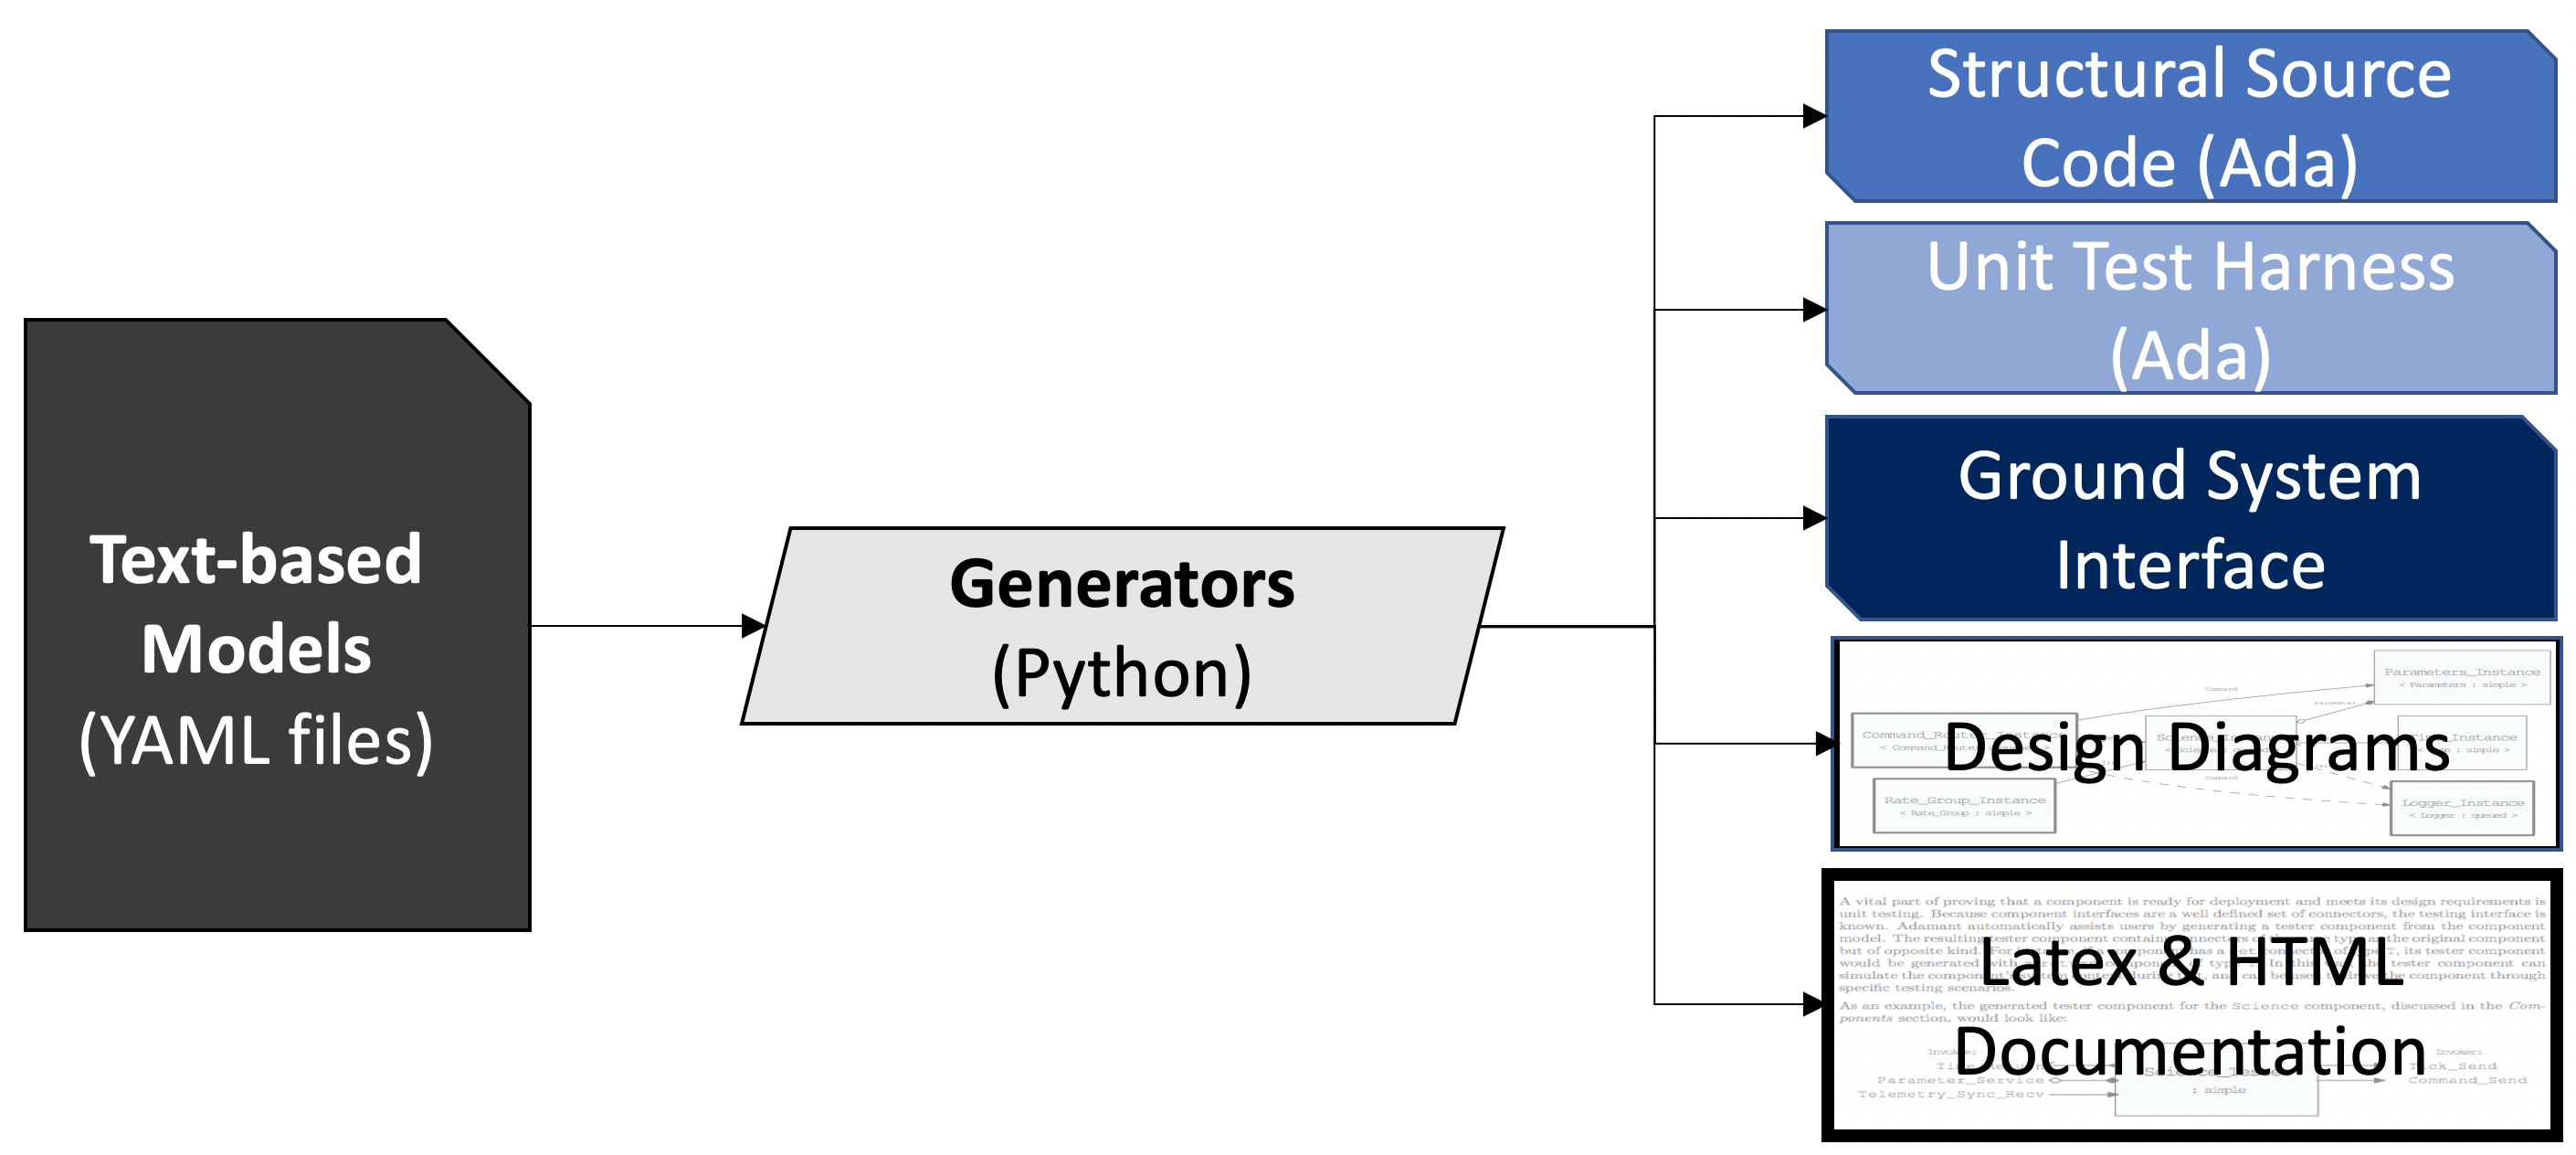
\includegraphics[width=0.85\textwidth,center]{images/modelbased.png}
  \caption{Adamant employs model-driven development. The system is modeled in text-based YAML files, and python generators are used to produce a variety of output products including autogenerated ``structural" code for the system, unit test harnesses, interface specifications, documentation, and visual diagrams.}
\end{figure}

The use of models within Adamant formalizes the traditional approach to software development. To build up a system using Adamant, an engineer first breaks down their system into \textit{components}, as described in the \href{https://github.com/lasp/adamant/blob/main/doc/architecture_description_document/architecture_description_document.pdf}{\textcolor{blue}{Architectural Description Document}}. This is often conducted on a whiteboard or piece of paper prior to codifying the design in the Adamant modeling language. Part of this process is carefully defining the set of \textit{packed types} that can be transmitted over specific connectors between components, see Section \ref{Packed Types}. Once these types are modeled, a component can be modeled, and implementation and unit testing can begin, see Section \ref{Components}. Using this process, engineers can build up an entire system of well-tested components and eventually assign these components to particular assemblies using an assembly model, see Section \ref{Assemblies}. At this point, the assemblies can be compiled and executed, and acceptance testing can be performed on the integrated software to ensure that it meets the requirements for the project.

\begin{figure}[H]
  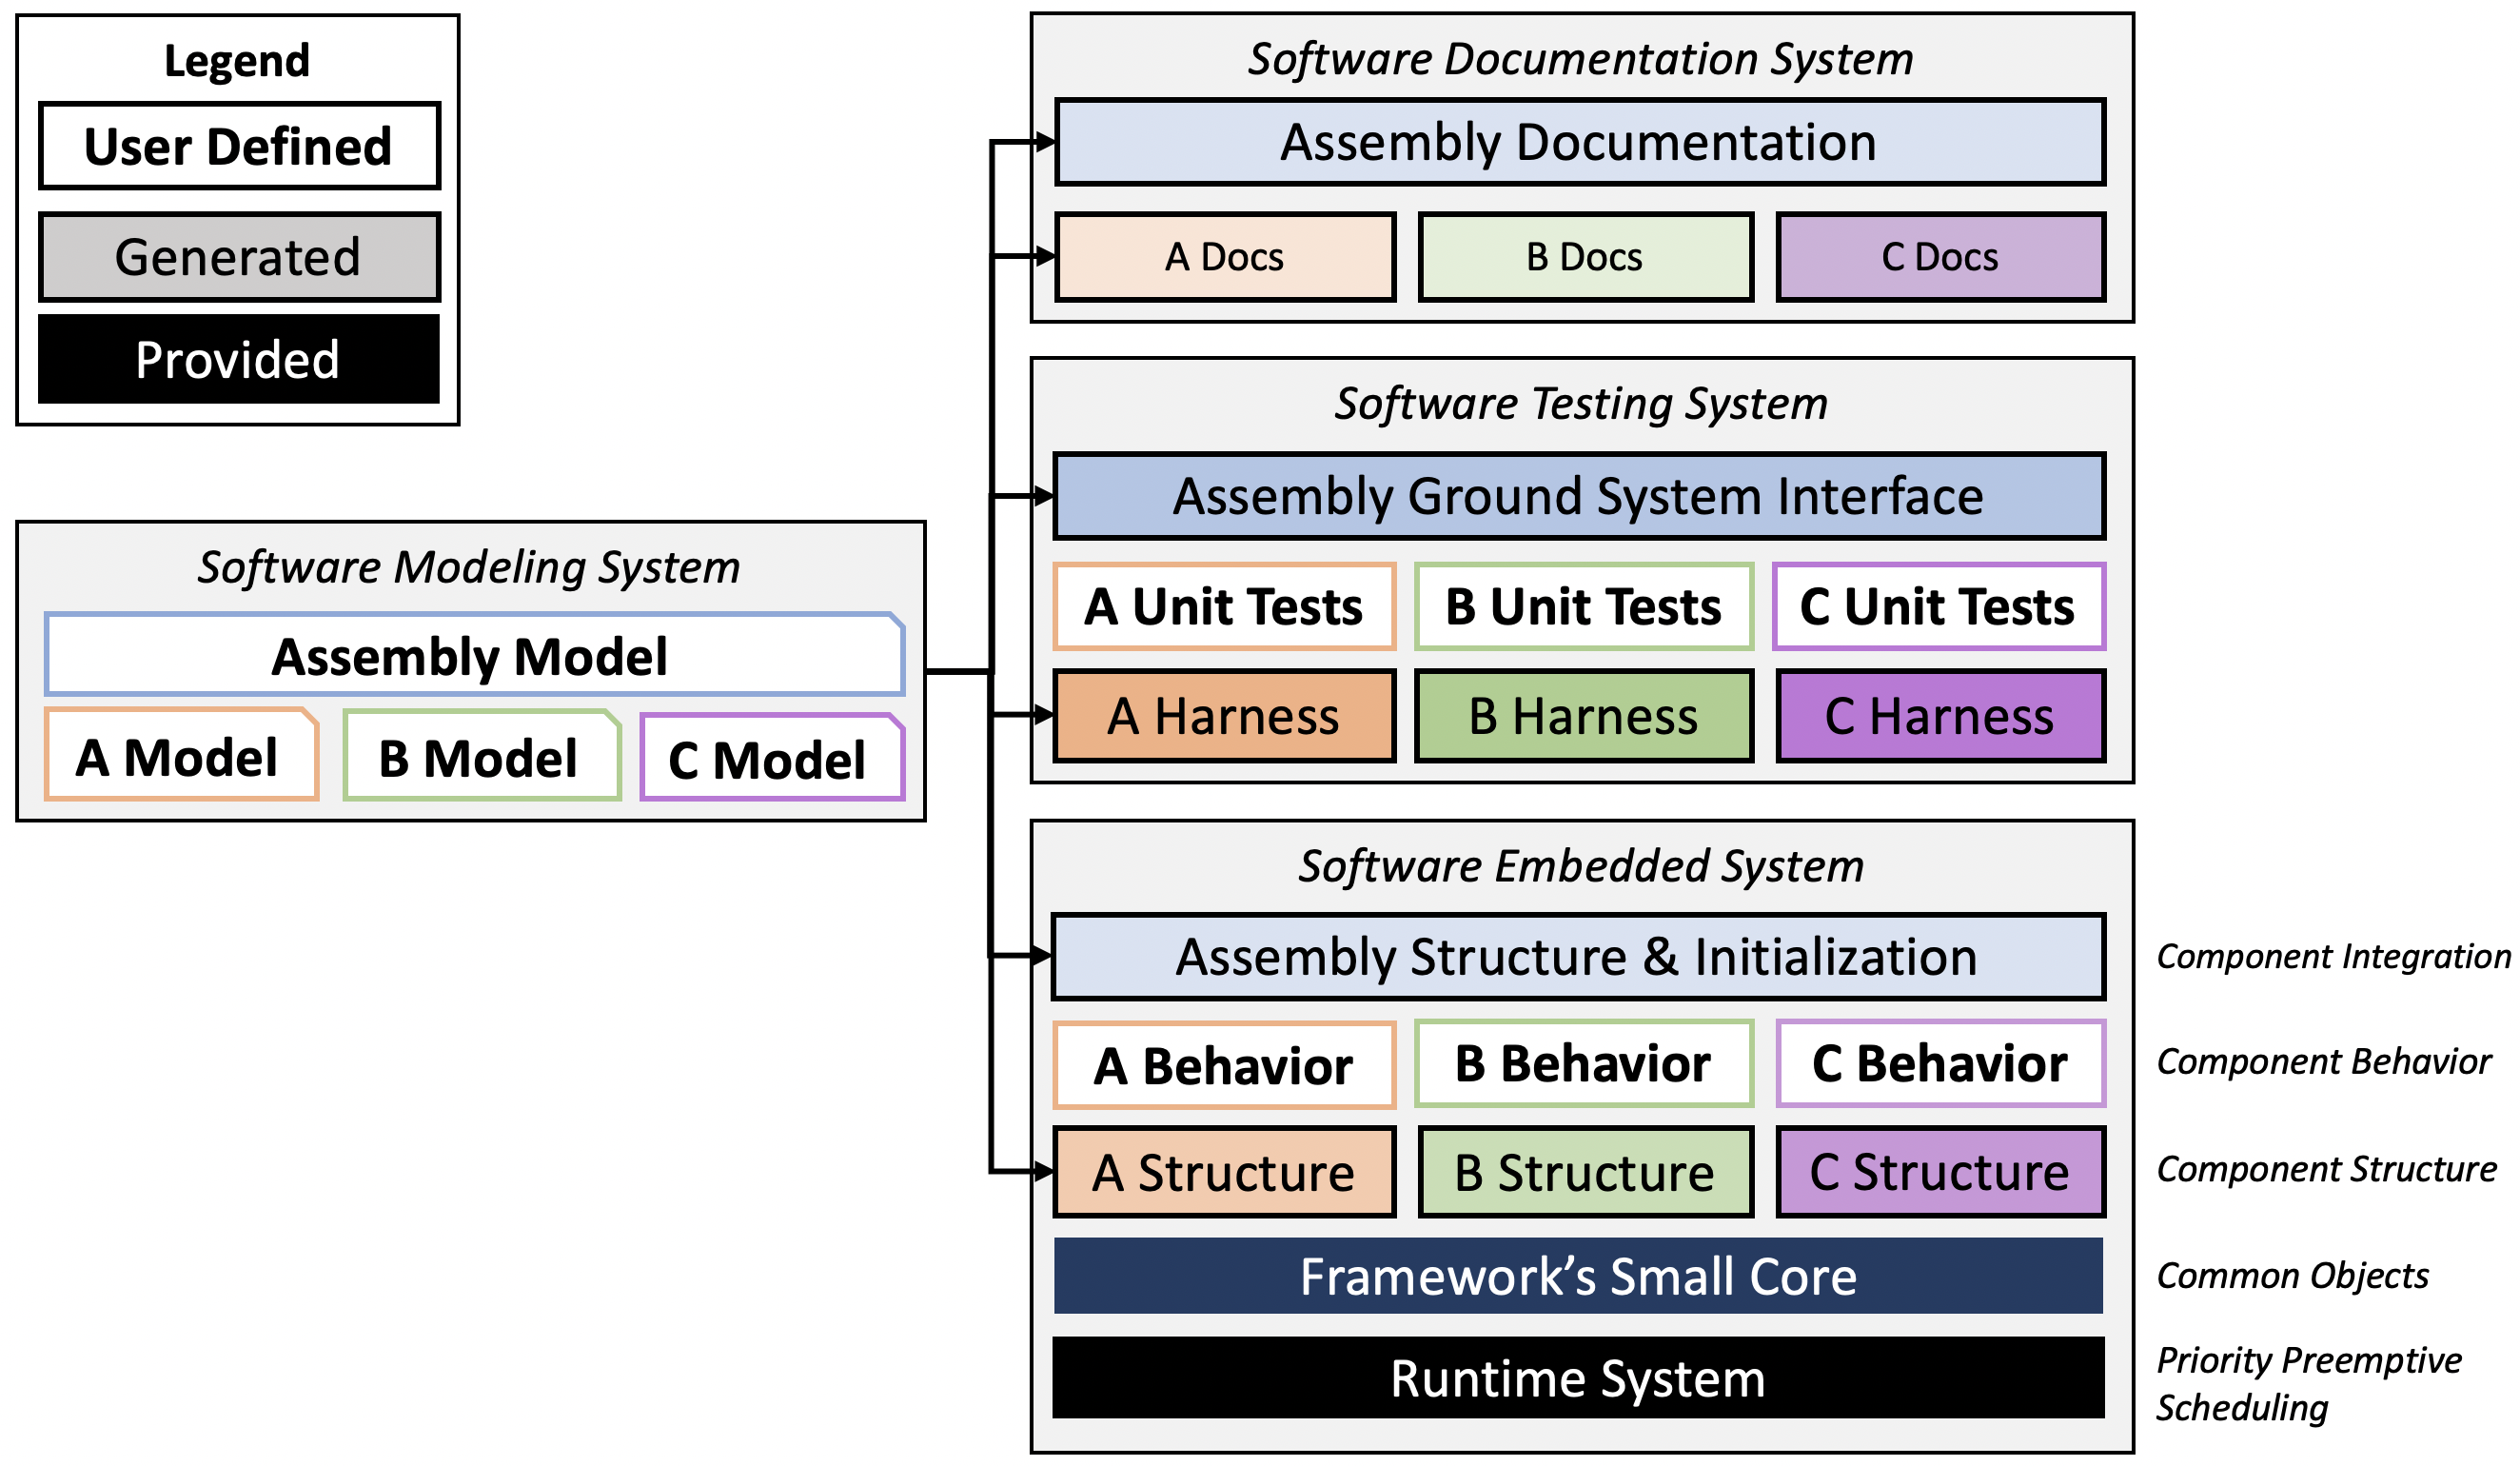
\includegraphics[width=1.0\textwidth,center]{images/architecturelayers.png}
  \caption{Adamant Architecture Layer Diagram for a simplified 3 component system. Modeling is used to ensure consistency between the embedded system, the testing system, and the software documentation.}
\end{figure}

The figure above shows an Adamant-based system with only 3 components. In the software modeling system, these 3 components (\textit{A}, \textit{B}, and \textit{C}) and the assembly they are part of are modeled. The assembly describes how the components are interconnected. From these models we can autogenerate the ``structural" code for each component that will execute on the embedded system. The autogenerated structural code defines a set of abstract subprograms that must be hand-coded by the engineer to define the component's behavior. From the assembly model, Adamant can autogenerate code that properly initializes all the components and connects them together. The assembly of components can then execute together on the embedded system on top of the Adamant framework's small set of core code and the language runtime system, described in more detail in the next section. In this way, the model defines the structure of the software running on the embedded system, and the programmer defines the behavior. \\

The models are also used to test the software thoroughly. For each component model, Adamant autogenerates a unit test harness. This harness consists of a ``reciprocal" component, which serves as an environment for unit testing each component in isolation. Again, Adamant defines the structure of the unit test harness, but the programmer defines the behavior, or in this case, the test cases to run. Using the assembly model, Adamant can autogenerate the interface for a ground system. This interface definition usually consists of the protocol and packet layout for communicating with the embedded system. In this way, the assembly model allows the programmer to begin high-level testing with confidence that the communication protocols on both sides of the system match. \\

Finally, documentation for each component and the assembly as a whole can be directly generated from the models. A significant amount of information can be understood from these autogenerated documents because of the precise nature of the Adamant modeling system. Human-written documentation can also be added to augment the autogenerated. The documentation is guaranteed to be up to date and reflective of the actual embedded software design because both are generated from the same model source. \\

Adamant embraces a holistic approach to modeling. Not only are components and assemblies modeled, but data types, commands, telemetry, parameters, unit tests, and even requirements are part of the modeling system. The result is that systems designed using Adamant end up having a significant portion of the underlying code structure automatically generated. It is not uncommon for 70\% of the total software for a project to be autocode. \\
 
The advantage of using models during the development process is that they ease many of the most challenging aspects of writing good software. Some of the key topics are discussed below. \\

\textbf{Effective Communication of Design} \\

Communicating design ideas in software among a group of software engineers is difficult on its own. Presenting these ideas to a broader audience of engineers, which is common in fields like aerospace, is even more challenging. The Adamant modeling system consists of a visual domain-specific language that is described in the \href{https://github.com/lasp/adamant/blob/main/doc/architecture_description_document/architecture_description_document.pdf}{\textcolor{blue}{Architectural Description Document}}. This language is simple to understand and explain, even to engineers unfamiliar with the details of software development. The notations in Adamant component diagrams have well defined semantics. The advantage is that when debating solutions to software problems, engineers find it easier to express their ideas, and less time is wasted on misunderstandings. \\

\textbf{Complete and Accurate Documentation} \\

Documentation is often neglected in the design of software. Weak or nonexistent documentation is a common problem. This can hinder effective review of the design and makes familiarizing new engineers on a project difficult. Because of Adamant's holistic approach to modeling, adequate documentation can often be generated straight from the model with a single command, see Section \ref{Component Documentation}. Furthermore, this documentation is guaranteed to be reflective of the actual implementation since both the code structure and the documentation are generated from the same model.  \\

\textbf{Interface Control Management} \\

Embedded systems are usually controlled through protocols managed by an Interface Control Document (ICD). For spacecraft, this includes command and telemetry definitions. Since these interface entities are modeled in Adamant, both sides of the interface can be generated using the Adamant modeling and generator system. For instance, if a command is described in an Adamant model, code can be generated in Adamant to allow the system to route and execute that command, see Section \ref{Commands}. In addition, the proper command packet definition can be generated for the ground system so that it can send the properly formatted command. In this way, the communication protocols on both sides can be generated from the same model. This ensures consistency and reduces the challenge of integrating two complex systems. \\

\textbf{Unit Testing Assistance} \\

Since the interface of a component is known in the model, Adamant can autogenerate a ``reciprocal" component that can be used to unit test, see Section \ref{Component Unit Testing}. The ``reciprocal" component contains the exact opposite connector definitions of the component under test, and acts as the perfect interface for interacting with the component in an isolated unit testing environment. This property makes unit testing components in Adamant straightforward to implement and understand. \\

\textbf{Code Clarity} \\

Using a software framework often requires the developer to write a lot of boilerplate code to follow the design patterns for that framework. Too much boilerplate code is frowned upon because it makes code less readable, and is often prone to copy and paste errors. Models allow Adamant to manage the entire ``structural" layer of the software. That structural layer defines what each component looks like and how the components communicate with each other. All of the code necessary to create this structure is autocoded into an abstract base package. This autocode serves a few important purposes. First, it encapsulates the structural code and, because it is generated, is much less prone to defects. Second, it declares abstract subprograms that the developer must hand-code to implement the component's behavior. This ensures that what the designer specifies in the model truthfully gets implemented in the code. Any deviation results in a compilation error. Finally, this process results in hand-code that has a high level of clarity, as it only shows the behavioral logic of the component. The structural code, hidden within the autocoded abstract base package, rarely needs to be scrutinized, since the same exact semantics are described in the model and the visual diagrams generated from it. This entire process is described in Section \ref{Components}.

\subsection{Ada as Implementation Language}

The implementation language for Adamant is the Ada 2012 programming language. It is recognized that the most significant obstacle in the adoption of the Adamant framework is likely the use of Ada. Since C or C++ are typically chosen for embedded systems, especially in the U.S., the decision to use Ada for Adamant necessitates justification.

The objective of Adamant is to produce reliable and reusable embedded, real-time software. In this theme, the utility of Ada and Adamant align. The comparison of Ada to C-like languages is best summarized by John Barnes in the introduction to \href{https://www.adacore.com/uploads/books/pdf/SafeSecureAdav2015-covered.pdf}{\textcolor{blue}{Safe and Secure Software}}:

\vspace{5mm} %5mm vertical space
\begin{quote}
One of the trends of the second half of the twentieth century was a universal
concern with freedom. But there are two aspects of freedom... Maybe A would like the freedom \textit{to} smoke in a pub
whereas B wants freedom \textit{from} smoke in a pub. Concern with health in this
example is changing the balance between these freedoms. Maybe the twenty-first century will see further shifts from “freedom to” to “freedom from”. \\

In terms of software, the languages Ada and C have very different attitudes towards
freedom. Ada introduces restrictions and checks, with the goal of providing
freedom from errors. On the other hand C gives the programmer more freedom,
making it easier to make errors. \\

One of the historical guidelines in C was “trust the programmer”. This would
be fine were it not for the fact that programmers, like all humans, are frail and
fallible beings. Experience shows that whatever techniques are used, it is hard to
write “correct” software. It is good advice therefore to use tools that can help by
finding bugs and preventing bugs. Ada was specifically designed for this
purpose. 
\end{quote}
\vspace{5mm} %5mm vertical space

Ada was designed from the ground up for embedded and real-time systems in the 1970s in an effort to promote safe and modular programming. Since then, the Ada language has expanded to include full concurrency, object-oriented features, and a formally provable subset called SPARK.

During Adamant's inception, the choice of language was a thoroughly debated and researched topic. The implementation of Adamant requires several important features in a programming language. The features necessary to support the architecture include:

\vspace{5mm} %5mm vertical space
\begin{spacedenumerate}
  \item A tasking system that contains a priority-preemptive scheduler
  \item Object-oriented features, particularity inheritance and abstract classes
  \item The ability to create highly reliable software
\end{spacedenumerate}
\vspace{5mm} %5mm vertical space

The following paragraphs explain how Ada fulfills these criteria compared to other languages, such as C/C++. \\

\textbf{Tasking Support:} \\

For embedded systems that need tasking support, a real time operating system (RTOS) is generally used such as VxWorks, RTEMS, FreeRTOS, etc. This is necessary in languages like C and C++ because they do not have constructs for tasking contained within the language. Instead, they must call into an RTOS API to spawn tasks and interact between tasks in a thread-safe manner.

In contrast, tasking, task synchronization, and thread-safe data sharing is built directly as first-class syntax into the Ada programming language. An underlying runtime system implements the tasking semantics. The runtimes used by Adamant are based on the \href{http://www.open-std.org/JTC1/SC22/WG9/n424.pdf}{\textcolor{blue}{Ravenscar Profile}}, which is a committee-designed profile that defines a subset of the Ada tasking system, designed specifically for safety-critical, hard real-time computing. The use of concurrency is explicit, and thread safety is achieved through lightweight \textit{protected objects}. Unlike C or C++ where mutual exclusion is achieved through semaphores and mutex locks, in Ada, shared variables are encapsulated and declared \textit{protected}. Access to these variables is expressed through the use of read-only functions, write-protected procedures, and synchronized entries. The compiler ensures mutual exclusion and guarantees deadlock-free execution by code insertion, which results in low overhead execution. This implementation produces a runtime that is both deterministic and small, making it straightforward to understand.

Using Ada instead of C/C++ relieves the programmer of needing to choose, understand, configure, and deploy a real-time operating system, most of which are much more complicated than the Ada Ravenscar runtimes. This reduces the complexity of the execution stack, making the system easier to understand and control by developers. It also relieves Adamant from needing an additional operating system abstraction layer (OSAL) to allow it to work with multiple RTOS implementations, which would certainly be in a requirement in a C or C++ implementation.

In regards to Adamant, Ada provides lean tasking support on top of bare-metal hardware using only the Ada language syntax. This simplifies the system, making it easier to manage and configure, and most importantly, easier to validate. \\

\textbf{Full Featured:} \\

Adamant requires a fully featured, object-oriented language to provide the proper compile-time guarantees that the modeling language expects. Ada is a very mature language with many of the popular features found in Java and C++. The language fully supports object-oriented design patterns, including inheritance, polymorphism, dynamic dispatching, overriding, and multiple-inheritance via mix-ins. The language is fully modular and supports separate compilation and privatization of code. It also includes features such as generics (similar to templates in C++) and interfaces, which greatly enhance code reusability. All of these features make it suitable for use in a reusable framework such as Adamant.

It should be noted that Ada compilers used with Adamant (usually \texttt{gcc}) compile to the same object code as C/C++. Interfacing between the languages is not difficult. Importing C/C++ libraries into Adamant is fully supported.

Because Ada uses the same object code as C/C++, it also uses the same back-end compilation optimizations. This makes Ada execute as fast as C/C++, with the caveat that Ada inserts extra runtime checks into the final executable. These runtime checks implement the semantics of the strong Ada type system, discussed more below. Runtime checks are included to make the code more robust, but can be turned off for performance-critical sections of code if execution time becomes a concern. \\

\textbf{Reliable:} \\

\begin{wrapfigure}{r}{0.40\textwidth}
  
\includegraphics[width=0.35\textwidth]{images/ada.jpg}
\end{wrapfigure}

Ada is designed from the ground up to support highly reliable computing on embedded systems. The most differentiating feature of Ada compared to other embedded languages is its rich and strong type system. The type system gives the programmer tools to create powerful abstractions. When provided to the compiler, these definitions aid in the automatic detection of many logical and design errors before they can become bugs. Ada provides compile-time and runtime safety checks of variables against their valid ranges for all types upon assignment or type conversion. Valid ranges for any type can be set by the programmer through use of a \textit{range constraint}. This feature allows the Ada compiler and runtime to detect array indexes that overflow, integers that go out of range, or enumeration types that become undefined. Notably, Ada lacks the widespread use of implicit type conversions, which are a common source of bugs in C/C++. An experienced Ada programmer embraces the expressiveness and strictness of the type system, using it to their advantage to write readable, defect-free code.

Ada also provides contracts, preconditions, postconditions, invariants, predicates, and assertions to allow the user to insert their own runtime checking in addition to what the language already provides. These constructs allow programmers to codify their assumptions about program execution, enforce the required state of variables at function call boundaries, and ensure that specific properties are upheld during program flow. These same constructs can also be used in the context of SPARK, a formally verifiable subset of Ada, to \textit{prove} that a program is free of runtime errors and meets its design requirements prior to execution. Adamant supports compilation and formal analysis of SPARK packages natively within the build system. SPARK packages can easily be developed, proved, and included within Adamant components. This allows users to formally prove important subsets of code for their projects. Note that Adamant core packages do not yet make heavy use of the SPARK language subset, but there are plans in the road map to begin converting the core to SPARK. 

Note that Adamant also provides support to link in C and C++ libraries. This allows for the clean reuse of legacy software or other external packages.

The learning curve for Ada is not unreasonably steep, especially if you have prior experience in a language like C++ or Java. Some of the best resources for diving into Ada are listed below:

\vspace{5mm} %5mm vertical space
\begin{spaceditemize}
  \item \href{https://learn.adacore.com/index.html}{\textbf{\textcolor{blue}{AdaCore Learn}}} - an interactive tutorial for learning Ada and SPARK basics
  \item \href{https://learn.adacore.com/courses/Ada_For_The_CPP_Java_Developer/index.html}{\textbf{\textcolor{blue}{Ada for the C++ or Java Developer}}} - a tutorial which teaches Ada features by comparing it to analogous features in C++ and Java
  \item \href{https://github.com/ohenley/awesome-ada}{\textbf{\textcolor{blue}{awesome-ada}}} - a curated list of awesome resources related to the Ada and SPARK programming language
  \item \href{https://en.wikibooks.org/wiki/Ada_Programming}{\textbf{\textcolor{blue}{Ada Programming Wiki}}} - a good resource for looking up Ada syntax and features
  \item \href{https://www.adacore.com/gems/}{\textbf{\textcolor{blue}{Ada Gems}}} - a set of blog posts demonstrating some of the most powerful and unique features of Ada
\end{spaceditemize}
\vspace{5mm} %5mm vertical space

\newpage
\section{Getting Started} \label{Getting Started}

This section contains what you need to know in order to get started with Adamant, including setting up the development environment and the basics of using the Adamant build system.

\subsection{Project Setup} \label{Project Setup}

One of the goals of Adamant is to produce highly modular embedded software. This goal does not end with the final deployed system, however. The same principles permeates through the implementation of Adamant and even to how one sets up their project. The Adamant framework itself is currently contained in a single repository that contains the generic code, generators, reusable components, and build system. What is not included in the Adamant repository is a final deployment of embedded software, known in Adamant as an \textit{assembly}. \textit{Assemblies}, by design, are always tailored to a specific project's requirements and target platform. In the Adamant ecosystem, this code is thought of as mission-specific code and thus is always contained in a repository separate from the Adamant framework, which is scoped to be generic and reusable. \\

When working with Adamant you will always have a minimum of 2 repositories, one that includes the Adamant framework, and another that contains your mission specific deployment, or \textit{assembly}. However, it may make sense to have 3, 4, or more repositories that make up your system. Adamant poses no limit on how you modularize your system, and allows you to tie the compilation of everything together via the \textit{build path}, which is detailed in Section \ref{The Build Path}. \\

Setting up a mission-specific repository is often different for each mission, based on the needs for that mission. Included with Adamant is an Example project which provides a good starting point for most projects. This section details how to set up Adamant with the \href{https://github.com/lasp/adamant_example}{\textcolor{blue}{example repository}} in order to get up and running with the system. Once you have had a chance to go through this guide and experiment with the example repository, it is recommended that you make a copy of the example repository and begin modifying it to form your own project repository. \\

\subsubsection{Project Directory}

Usually, all repositories for a project are cloned into a single ``project directory". This is not strictly necessary with Adamant, due to the flexibility of the build system, however the steps below present it this way and have been tested. The first step when getting started is to create a project directory and clone the Example and Adamant repositories:

\vspace{5mm} %5mm vertical space
\begin{minted}{text}
> mkdir project  # make project directory
> cd project
> git clone https://github.com/lasp/adamant_example.git
> git clone https://github.com/lasp/adamant.git
\end{minted}
\vspace{5mm} %5mm vertical space

This setup implies a flat structure, where the many repositories are stored within the root \texttt{project/} directory. Each repository has a separate history and configuration management. Keeping them in sync can be done via a versioning process, branch naming conventions, or any other myriad of ideas which are not discussed here and should be tailored for your program. Alternatively, one could use git submodules. The complexity of git submodules is not discussed here, but nothing in Adamant precludes you from working in that manner. \\

Now that we have the directory set up with the repositories, we need to set up the virtual development environment, described in the next section.

\subsubsection{Virtual Development Environment}

Adamant uses a virtual environment for development for a few reasons. First, using a virtual environment makes it easy to install all the necessary dependencies without cluttering up the host system. Secondly, it bypasses the classic ``it works on my machine" problem that is so prevalent in software development, since all developers are using the same exact machine. \\

Developers can be picky about the tools they install, the editors they use, and whether or not to use spaces or tabs (you should use spaces!). Adamant does its best to not force the use of any tool on any developer, with the exception of using \texttt{redo}, discussed in Section \ref{Using Redo}. To accomplish this, the Adamant virtual environment shares the project directory, discussed in the last section, between the host and the virtual machine. In this way, the developer can install whatever tools they want on either the host or the virtual machine, to interact with the system how they please. The only requirement is that you must run build commands, ie. \texttt{redo}, from within the virtual machine via the virtual environment GUI or an \texttt{ssh} session. \\

The virtual environment for Adamant is based on Linux, because it is ubiquitous, easy to configure, open source, and widely supported. Currently the virtual environment managed by \href{https://www.docker.com/}{\texttt{\textcolor{blue}{Docker}}}. To ensure that you use the most up to date instructions for setting up the example repository it is recommended you follow the repository specific directions stored in \href{https://github.com/lasp/adamant_example/blob/main/docker/README.md}{\textcolor{blue}{this README.md}}. Please follow those instructions to bring up your machine. \\

\subsubsection{Project Configuration} \label{Project Configuration}

Adamant provides a single configuration file that can be used to tailor the framework for a specific project. The default version of this configuration file is stored in \textit{config/adamant.configuration.yaml.original} and is shown below: \\

\textit{adamant.configuration.yaml.original:}
\yamlcodef{../../config/adamant.configuration.yaml.original}

As can be seen, most of the configuration available is changing the size of core types used within the system including commands, events, parameters, etc. As described in the comments, you can also add your own variables within this YAML file and then use them within your source code or YAML model definitions. \\

The Adamant framework will not function without a configuration file in place. To try out Adamant using the default configuration you can run:

\vspace{5mm} %5mm vertical space
\begin{minted}{text}
> cp adamant.configuration.yaml.original adamant.configuration.yaml
\end{minted}
\vspace{5mm} %5mm vertical space

You can now modify the values in \textit{adamant.configuration.yaml} to work for your project. Note that \textit{adamant.configuration.yaml} has been added to .gitignore, and should NOT be checked into your version control system if you intend on merging changes from your Adamant repository back into the framework root repository.

Version controlling the configuration file is usually desirable. To accomplish this, copy the Adamant default configuration into your project specific repository:

\vspace{5mm} %5mm vertical space
\begin{minted}{text}
> cp adamant.configuration.yaml.original /prj_dir/config/project.configuration.yaml
\end{minted}
\vspace{5mm} %5mm vertical space

You can now modify \textit{project.configuration.yaml} and version control it within your project directory. To tell Adamant to use this file instead of the default configuration file, you need to set the \texttt{ADAMANT\_CONFIGURATION\_YAML} variable, ie.

\vspace{5mm} %5mm vertical space
\begin{minted}{text}
> export ADAMANT_CONFIGURATION_YAML=/prj_dir/config/project.configuration.yaml
\end{minted}
\vspace{5mm} %5mm vertical space

It is advisable to include the export command above within your environment files that get sourced whenever a new shell is opened, ie. from .bashrc. \\

A good example for how to set up the configuration file for you project is to look at the \href{https://github.com/lasp/adamant_example/tree/main}{\textcolor{blue}{example repository}} which includes its configuration within the \textit{config/} directory, and sets the \texttt{ADAMANT\_CONFIGURATION\_YAML} variable using the \textit{env/setenv.sh} script.

\subsection{Adamant File Structure}

This section provides a brief tour of the Adamant repository layout so that a user may more easily find what they are looking for. Adamant is a framework that consists of many parts that all function together to help you write good embedded software. The main constituents are:

\vspace{5mm} %5mm vertical space
\begin{spaceditemize}
  \item \textbf{\textit{core code}} - hand-written (Ada) code that implements the foundational elements for the Adamant architecture; this code is compiled and run on the embedded target
  \item \textbf{\textit{components}} - reusable components that can be deployed to the embedded target
  \item \textbf{\textit{generators}} - the Adamant generator system, used for generating structural autocode, configuration files, diagrams, and documentation 
  \item \textbf{\textit{build system}} - the Adamant build system, used for compiling source code and documentation
  \item \textbf{\textit{ground code}} - hand-written (python and MATLAB) code that provides tooling to assist in testing the embedded system
  \item \textbf{\textit{environment}} - files for configuring and provisioning the Adamant development environment
\end{spaceditemize}
\vspace{5mm} %5mm vertical space

The most important directories in the Adamant repository are listed below with descriptions of what you can find in each:

\vspace{5mm} %5mm vertical space
\begin{spaceditemize}
  \item \textbf{\texttt{config/}} - Configuration files for tuning the Adamant framework to fit a specific project
  \item \textbf{\texttt{doc/}} - Adamant documentation including the Architectural Description Document, this User Guide, the Quick Start Guide, and more
  \item \textbf{\texttt{env/}} - environmental files to aid in provisioning and configuring the Adamant development environment
  \item \textbf{\texttt{gen/}} - Adamant generator system used for generating structural autocode, configuration files, diagrams, and documentation 
  \item \textbf{\texttt{gen/generators}} - python generators which tie in with the Adamant build system to create build rules for each generated file
  \item \textbf{\texttt{gen/models}} - python model classes which ingest and calculate all modeling information used by the generators
  \item \textbf{\texttt{gen/schemas}} - YAML schemas used to validate user model files prior to running generators 
  \item \textbf{\texttt{gen/templates}} - Jinja2 templates used in outputting various autocoded files
  \item \textbf{\texttt{gen/test}} - unit tests that verify the correct function of the Adamant generators
  \item \textbf{\texttt{gnd/}} - ground code (python) that provides tooling to assist in testing the embedded system
  \item \textbf{\texttt{src/}} - source code intended to be compiled and run on the embedded target
  \item \textbf{\texttt{src/components}} - source code for reusable components
  \item \textbf{\texttt{src/core}} - source code for Adamant core constructs: connectors, components, etc.
  \item \textbf{\texttt{src/data\_structures}} - source code implementing common Adamant data structures: queues, trees, etc.
  \item \textbf{\texttt{src/types}} - source code implementing common Adamant types: commands, parameters, etc.
  \item \textbf{\texttt{src/unit\_test}} - source code implementing Adamant unit test infrastructure: histories, smart assertions, etc.
  \item \textbf{\texttt{src/util}} - source code implementing various utility packages
  \item \textbf{\texttt{redo/}} - the Adamant redo-based build system, included is the build system core code and build rules for compiling source code, \LaTeX, Graphviz, and much more
  \item \textbf{\texttt{redo/rules}} - Adamant build rules
  \item \textbf{\texttt{redo/targets}} - supported Adamant build targets
\end{spaceditemize}
\vspace{5mm} %5mm vertical space

As discussed in Section \ref{Project Setup} the Adamant repository only contains the generic framework code, and expects a separate repository to use Adamant for a specific project. Provided with Adamant is the Example project which demonstrates how Adamant can be used for a specific application. The most important directories in that repository are listed below with descriptions of what you can find in each:

\vspace{5mm} %5mm vertical space
\begin{spaceditemize}
  \item \textbf{\texttt{config/}} - Adamant configuration file for the example project
  \item \textbf{\texttt{env/}} - files used to provision and configure the Example project environment
  \item \textbf{\texttt{src/}} - example repository source code for deployment to the embedded system
  \item \textbf{\texttt{src/assembly}} - executable assemblies for the Example project
  \item \textbf{\texttt{src/components}} - project-specific components for the Example project
  \item \textbf{\texttt{docker/}} - houses the Docker configuration which spawns the virtual environment for the Example project, also contains directions for setting up your machine
\end{spaceditemize}
\vspace{5mm} %5mm vertical space

Both repositories contain \textit{README.md} files in many directories that explain their contents further.

\subsection{Using the Build System} \label{Using the Build System}

Adamant uses a top-down, general purpose build tool called \href{https://redo.readthedocs.io/en/latest/}{\texttt{\textcolor{blue}{redo}}}. \texttt{redo} is designed in the spirit of the long-lived \texttt{make} program, but is much simpler and, surprisingly, much more powerful. See \href{https://redo.readthedocs.io/en/latest/}{{\textcolor{blue}{here}}} for the official documentation on \texttt{redo} and \href{https://github.com/dinkelk/redo}{{\textcolor{blue}{here}}} for the source code of the implementation used within Adamant. You can write custom \texttt{.do} scripts for redo anywhere in Adamant and expect them to function according to the \texttt{redo} documentation. Adamant itself, however, uses a sophisticated python based build system that utilizes \texttt{redo} under the hood to manage dependencies and rebuild logic. \\

The Adamant build system is largely ``discovery"-based. There are very few build system configuration files in Adamant, unlike what you might find within most build systems based on \texttt{make}, \texttt{CMake}, \texttt{scons}, etc. Instead, the build system looks at the filesystem and generates build rules based on the file types that it finds. To support this, Adamant uses specific file naming conventions that are used in the rest of this document. The build system looks for filenames of a specific format and generates rules that operate on that file type. What this means for an Adamant user is less time spent telling the build system how to build their code, and more time spent writing good software. \\

Similar to python, the Adamant build system works with the concept of a \textit{build path} in the form \texttt{\url{/path/to/directory1:/path/to/directory2:etc}}. Source code (and model files) found in the build path can see each other during compilation and thus can interact via Ada \texttt{with} statements or other model based import mechanisms to be presented. The \textit{build path} is automatically calculated by \texttt{redo} prior to running any \texttt{redo} command, so the user does not have to think too much about it. However, the build path can be fine tuned, and may need to be, for various reasons. See Section \ref{The Build Path} for more details. \\

The Adamant build system also supports compilation and cross-compilation for many different platforms from the same set of source code. This is supported through the use of \textit{build targets}. See section \ref{The Build Target} for more details.

\subsubsection{Using Redo} \label{Using Redo}

The primary method for interacting with the Adamant build system is through \href{https://redo.readthedocs.io/en/latest/}{\texttt{\textcolor{blue}{redo}}} commands run at the command line. Integration of the Adamant build system within an IDE ecosystem is work that has yet to be started. \\

\texttt{redo} is run by providing it a single argument that is the item to build, also referred to as the \textit{command}. When \texttt{redo} is run, the program searches for a build rule that matches your argument, executes it, and tracks any dependencies needed to rebuild it intelligently in the future.  If no argument is provided then \texttt{redo} assumes you want to build the \texttt{all} command. In Adamant, when the \texttt{all} command is run, the build system attempts to build any object and most source code that can be constructed within that directory. \\

It should be noted that most of the discussion below is specific to the Adamant build system, which \textit{uses} \texttt{redo}. These are NOT features of \texttt{redo} itself, which is a rather simple, but powerful, tool. \\

Below are some example \texttt{redo} commands that you can run within Adamant:

\vspace{5mm} %5mm vertical space
\begin{minted}{text}
> redo                       # run "redo all" in this directory
> redo all                   # run "redo all" in this directory
> redo ../../all             # run "redo all" two directories above this one
> redo output.txt            # tell redo to build output.txt in this directory
> redo build/src/file.txt    # tell redo to build file.txt in build/src
\end{minted}
\vspace{5mm} %5mm vertical space

In Adamant, all autogenerated source code, documentation, diagrams, compiled objects, and compiled executables is constructed in a \textit{build/} directory directly below the YAML model or source used to generate the output. Below is a list of common subdirectories you might find in a \textit{build/} directory and what is contained in each:

\vspace{5mm} %5mm vertical space
\begin{spaceditemize}
  \item \textbf{\texttt{build/src}} - autogenerated source files, which are automatically added to the build path if the directory containing \textit{build/} is in the build path.
  \item \textbf{\texttt{build/template}} - autogenerated source files that are meant to be copied out and used as starting points (ie. ``templates") for handwritten code
  \item \textbf{\texttt{build/obj/Linux}} - compiled object files for the \texttt{Linux} target
  \item \textbf{\texttt{build/obj/Linux\_Test}} - compiled object files for the \texttt{Linux\_Test} target
  \item \textbf{\texttt{build/bin/Linux}} - compiled executable files (\textit{.elf}) for the \texttt{Linux} target
  \item \textbf{\texttt{build/bin/Linux\_Test}} - compiled executable files (\textit{.elf}) for the \texttt{Linux\_Test} target
  \item \textbf{\texttt{build/py}} - autogenerated python source files
  \item \textbf{\texttt{build/m}} - autogenerated MATLAB source files
  \item \textbf{\texttt{build/html}} - HTML documentation
  \item \textbf{\texttt{build/pdf}} - PDF documentation
  \item \textbf{\texttt{build/tex}} - Latex files used to create PDF documentation
  \item \textbf{\texttt{build/metric/Linux}} - metrics reports for source code used to build a \texttt{Linux} object
  \item \textbf{\texttt{build/csv}} - CSV files
  \item \textbf{\texttt{build/svg}} - Scalar Vector Graphics diagrams
  \item \textbf{\texttt{build/dot}} - Graphviz "dot" specification files for generating diagrams
  \item \textbf{\texttt{build/eps}} - Encapsulated PostScript files used to present images in PDF files
  \item \textbf{\texttt{build/png}} - PNG images
\end{spaceditemize}
\vspace{5mm} %5mm vertical space

As can be seen, most output files are generated in a directory that contains the file extension for that file type. The \textit{build/obj/} and \textit{build/bin/} directories are unique in that they always contain another set of subdirectories that specify the \textit{build target} that they were compiled for. More details on \textit{build targets} can be found in Section \ref{The Build Target}. \\

The use of \textit{build/} directories also makes ``cleaning" fast. To remove all generated outputs you can run:

\vspace{5mm} %5mm vertical space
\begin{minted}{text}
> redo clean     # remove any build/ directories in this directory
> redo clean_all # remove any build/ directories for entire repository
\end{minted}
\vspace{5mm} %5mm vertical space

One of the most useful \texttt{redo} commands in Adamant is \texttt{redo what}, which shows you all the possible redo commands you can run in your current directory. Below is an example of running \texttt{redo what} from Adamant's \textit{src/core/component} directory:

\vspace{5mm} %5mm vertical space
\begin{minted}{text}
> redo what # show "redo" commands that can be run in this directory
redo  what
redo all
redo clean
redo clean_all
redo clear_cache
redo templates
redo publish
redo targets
redo prove
redo analyze
redo style
redo pretty
redo test_all
redo coverage_all
redo build/metric/Linux/component.adb.txt
redo build/metric/Linux/component.ads.txt
redo build/metric/Linux/component.o.txt
redo build/obj/Linux/component.o
\end{minted}
\vspace{5mm} %5mm vertical space

We can see that in this directory, \texttt{redo} has found a lot of valid build commands. We can run commands to compile an object, \textit{build/obj/Linux/component.o}, or even run some code metrics on a source code file, \textit{build/metric/Linux/component.adb.txt}

Adamant also provides a set of build commands that can be used in almost any project directory. These are described below:

\vspace{5mm} %5mm vertical space
\begin{spaceditemize}
  \item \textbf{\texttt{redo what}} - show available redo commands to run in this directory
  \item \textbf{\texttt{redo all}} - build all objects, documentation, and source code (most) that can be built from this directory
  \item \textbf{\texttt{redo path}} - runs \texttt{redo all} from all directories in the build path
  \item \textbf{\texttt{redo recursive}} - runs \texttt{redo all} from this directory and all below it
  \item \textbf{\texttt{redo clean}} - removes all \textit{build/} directories from this directory and all below it
  \item \textbf{\texttt{redo clean\_all}} - removes all \textit{build/} directories from this entire repository
  \item \textbf{\texttt{redo clear\_cache}} - remove the model cache that the build system uses to increase performance, see Section \ref{The Model Cache}
  \item \textbf{\texttt{redo templates}} - finds and builds all autocoded templates (in \textit{build/template/}) that can be built from this directory
  \item \textbf{\texttt{redo test\_all}} - finds and runs all unit tests from this directory an all below it. Note: Add a \textit{.skip\_test} file to a directory to exclude it from being run by \texttt{redo test\_all}.
  \item \textbf{\texttt{redo coverage\_all}} - finds and runs all unit tests from this directory an all below it and generates coverage reports for each. Note: Add a \textit{.skip\_test} or \textit{.skip\_coverage} file to a directory to exclude it from being run by \texttt{redo coverage\_all}.
  \item \textbf{\texttt{redo publish}} - builds all autocoded documentation from this directory an all below it, and copies over the ``published" version of that documentation
  \item \textbf{\texttt{redo targets}} - shows a list of all available \textit{build targets}, see Section \ref{The Build Target}
  \item \textbf{\texttt{redo prove}} - runs \texttt{GNATprove} to analyze any SPARK code found within the current directory, see Section \ref{Creating a SPARK Package}
  \item \textbf{\texttt{redo test}} - compiles and runs a unit test - note: this command is only available if a \textit{test.adb}, \textit{test.c(pp)}, or \textit{test.py} file is found in this directory
  \item \textbf{\texttt{redo run}} - compiles and runs a main program - note: this command is only available if a \textit{main.adb} file is found in this directory
  \item \textbf{\texttt{redo style}} - compiles all objects found in this directory with coding style checks enabled
  \item \textbf{\texttt{redo pretty}} - ``pretty" formats all hand-written code found in this directory and saves them in \textit{build/template/}
  \item \textbf{\texttt{redo analyze}} - runs a static analyzer on all code found in this directory
\end{spaceditemize}
\vspace{5mm} %5mm vertical space

One unique feature of \texttt{redo} is that it prints what it is currently building while it runs, and also shows you each build rule's dependencies via indentation. Below is an example of \texttt{redo} being run to generate the component documentation for the \texttt{Command\_Router} component (run in \textit{src/components/command\_router/doc}) Some of the output has been removed for brevity:

\vspace{5mm} %5mm vertical space
\begin{minted}{text}
> redo build/pdf/command_router.pdf
redo  build/pdf/command_router.pdf
redo    ../build/eps/command_router.eps
redo    build/tex/command_router_init.tex
redo    build/tex/command_router_description.tex
redo    build/tex/command_router_events.tex
redo    build/tex/command_router_connectors.tex
redo    build/tex/command_router_requirements.tex
redo    build/tex/command_router_commands.tex
redo    build/tex/command_router_types.tex
redo      ../../../types/event/build/tex/event_header.tex
redo      ../../../types/event/build/tex/event.tex
redo      ../../../types/data_products/build/tex/data_product.tex
redo      ../../../types/data_products/build/tex/data_dependency.tex
redo      ../../../types/command/build/tex/command_id_status.tex
redo      ../../../types/command/build/tex/invalid_command_info.tex
redo      ../../../types/command/build/tex/command_id.tex
redo      ../build/tex/command_router_arg.tex
\end{minted}
\vspace{5mm} %5mm vertical space

As can be seen, building \textit{command\_router.pdf} depends on an autogenerated \textit{.eps} diagram and various autogenerated Latex (\textit{.tex}) files. One of these Latex files, \textit{build/tex/command\_router\_types.tex}, in turn, depends on another whole set of autogenerated Latex files. Using the \texttt{redo} output a user can inspect the autogenerated dependencies being built for the command they are running which can aid in understanding how their output is being constructed. \\

For speed, \texttt{redo} can also run build rules in parallel using the \texttt{-j} option. Here is an example telling \texttt{redo} to use 3 CPUs simultaneously to build:

\vspace{5mm} %5mm vertical space
\begin{minted}{text}
> redo -j3 # run "redo all" using 3 CPU cores
\end{minted}
\vspace{5mm} %5mm vertical space

Note that when using this option the printed output order is not preserved, so no dependency information can be gleaned from it. Also, parallel builds should be considered an experimental and unstable feature, and should not be used for critical compilations. \\

For more \texttt{redo} options you can run:

\vspace{5mm} %5mm vertical space
\begin{minted}{text}
> redo -h  # display help for redo
\end{minted}
\vspace{5mm} %5mm vertical space

Very rarely, \texttt{redo} can get itself into an unknown state. If things are not behaving correctly you can wipe out the redo database, and force things to rebuild fresh, which often fixes any issues that arise.To be safe, you can also remove the model cache that the build system uses to increase performance. The best procedure to do this is:

\vspace{5mm} %5mm vertical space
\begin{minted}{text}
> rm -rf ~/.redo      # remove the redo database
> redo clean_all      # clean the entire repository
> redo clear_cache    # remove the model cache
> redo <your_command> # retry the redo command that was not working
\end{minted}
\vspace{5mm} %5mm vertical space

\subsubsection{The Build Target} \label{The Build Target}

The Adamant build system supports building binary object and executable files for multiple target platforms. For instance, two binaries built from the same source code can be constructed in both a native Linux format and an embedded ARM-based target. Determining which platform a binary is compiled for is determined by the \textit{build target}. In Adamant, the \textit{build target} is a compilation configuration that determines the following:

\vspace{5mm} %5mm vertical space
\begin{spacedenumerate}
  \item The set of code that is used to compile for the target, ie. \textit{the build path} discussed in the next section
  \item The platform for which the code is being compiled, ie. the name of the compiler, linker, and binding programs
  \item The compiler configuration determined by compiler options (flags)
  \item The Ada \textit{runtime} that the application code will run on top of
\end{spacedenumerate}
\vspace{5mm} %5mm vertical space

The Ada compiler used in Adamant is generally GNAT based \texttt{gcc} for Native Linux compiles, and \texttt{gcc}-based cross compilers for embedded targets (ie. \texttt{arm-eabi-gcc} for ARM). The compiler, compilation flags, and runtime are all determined by the \textit{build target}. The Adamant \textit{build path} determines which source code is compilable for a given \textit{build target} and is discussed in the following section. To add a custom build target for your system see Section \ref{Adding a Build Target} for details. \\

As background, it is important to understand the Ada runtime system, on top of which an Ada application runs. The Ada runtime provides the tasking logic necessary to implement the Ada language. Adamant utilizes bare metal runtimes provided by AdaCore, which come in the following flavors:

\vspace{5mm} %5mm vertical space
\begin{spaceditemize}
  \item \textbf{\texttt{ZFP}} - The zero-footprint runtime only allows the non-tasking semantics of the Ada language. The resulting program must be single-threaded. This runtime is designed for formal software certification and/or for systems that are severely resource constrained.
  \item \textbf{\texttt{SFP}} - The small footprint runtime implements a restricted subset of the Ada tasking system described by the Ravenscar profile. This runtime provides minimal tasking capabilities, without exception propagation, to make formal software certification feasible.
  \item \textbf{\texttt{Full}} - The full runtime implements a restricted subset of the Ada tasking system described by the Jorvik profile. This profile is a slightly relaxed version of the Ravenscar profile, and allows exception propagation, designed for use on most embedded systems that do not require formal software certification. Note that the Jorvik profile is still very minimal compared to the full Ada language semantics which offers \texttt{select} statements, \texttt{rendezvous}, etc. These more flexible facilities are still not available in the Jorvik profile.
\end{spaceditemize}
\vspace{5mm} %5mm vertical space

There is also the native runtime, such as compiling directly for Linux or MacOS, which uses underlying operating system calls to implement the Ada tasking system. Adamant ensures that all software produced adheres to the Ravenscar profile (except for unit tests), such that either an SFP or Full runtime can be used. The ZFP runtime is not currently supported by Adamant components, but can be added if a project needs it in the future. \\

As previously mentioned, \textit{build targets} also determine the compiler options in effect during compilation. In an attempt to standardize build targets within Adamant, the following table describes the different compiler \textit{modes} used. A compiler mode is simply a standardized set of compilation options, used to make talking about compilation easier among developers.

\captionof{table}{Adamant Standard Compilation Modes}
\begin{xltabular}{\textwidth}{ | l | c | c | X | X | X | }
  \hline
  \textbf{Mode Name} & \shortstack{\textbf{Runtime} \\ \textbf{Mode}} & \shortstack{\textbf{Optimiz-} \\ \textbf{ation}} & \shortstack{\textbf{Validity} \\ \textbf{Checking}} & \shortstack{\textbf{Configuration} \\ \textbf{Pragmas}} & \textbf{Purpose} \\ \hline
  \textbf{Production} & Production & \shortstack{-O2 and \\ inlining} & \shortstack{RM-defined \\ checks \\ (-gnatVd)} & Ravenscar & Used for deployed system in production. \\ \hline
  \textbf{Development} & Production & \shortstack{-O2 and \\ inlining} & \shortstack{All checks \\ (-gnatVa)} & Ravenscar, Initialize\_Scalars* & Used for most development testing on target system. \\ \hline
  \textbf{Debug} & Debug & -O0 & \shortstack{All checks \\ (-gnatVa)} & Ravenscar, Initialize\_Scalars & Used for debugging hard to track down issues. \\ \hline
  \textbf{Test} & Debug & -O0 & \shortstack{All checks \\ (-gnatVa)} & Initialize\_Scalars & Linked with AUnit for unit test. \\ \hline
  \textbf{Coverage} & Debug & -O0 & \shortstack{All checks \\ (-gnatVa)} & Initialize\_Scalars & Same as Test with coverage options enabled. \\ \hline
\end{xltabular}

Note that runtimes can be compiled with debug flags (\textit{Debug} mode) or without debug flags and with optimization enabled (\textit{Production} mode). Optimization and back-end inlining is applied to the application code in \textit{Production} and \textit{Development} builds, but is not applied in any other modes. More information on Ada compiler optimization can be found \href{https://gcc.gnu.org/onlinedocs/gcc-4.6.2/gnat_ugn_unw/Switches-for-gcc.html}{\textcolor{blue}{here}}. \\

Ada allows the configuration of runtime validity checks within the language. It is advisable to keep the default reference manual checks on in \textit{Production} mode to prevent any undefined behavior. In all other modes, all validity checking provided by GNAT is enabled. This provides much more extensive type checking than the default Ada checking, which can help track down hard to find bugs at the cost of extra code insertion into the binary. More information on validity checks within the Ada compiler can be found \href{https://gcc.gnu.org/onlinedocs/gcc-4.6.2/gnat_ugn_unw/Validity-Checking.html#Validity-Checking}{\textcolor{blue}{here}}. \\

Ada also allows the user to restrict the use and behavior of the language by specifying configuration pragmas that apply to all the source code in the compilation. In \textit{Production}, \textit{Development}, and \textit{Debug} mode the Ravenscar profile is applied which restricts the tasking semantics allowed in the source code. This ensures that these builds will work with embedded runtimes, which support limited tasking semantics of the Ada language. Ravenscar is not enforced in \textit{Test} and \textit{Coverage} mode, to enabled more elaborate unit testing setups. All modes except \textit{Production} (*and \textit{Development} on bareboard targets) specify the pragma \texttt{Initialize\_Scalars}, which when used in conjunction with all validity checks enabled (\textit{-gnatVa}) can greatly aid in the detection of uninitialized variable bugs. Note that this pragma purposely initializes all uninitialized variables to values outside the range for that type in order to force runtime errors for any variables that are used prior to initialization. See this \href{https://www.adacore.com/uploads/techPapers/rtchecks.pdf}{\textcolor{blue}{case study}} to explore the benefits of \texttt{Initialize\_Scalars} pragma. \\

In summary, the \textit{Production} mode should be used for deployed software on target hardware. The \textit{Development} mode should be the most commonly used mode, as it should be preferred for most development and testing on target hardware. The \textit{Debug} mode turns off optimization of application and runtime code to make tracking down hard to find bugs easier. The \textit{Test} and \textit{Coverage} modes are designed for unit testing. These modes are an attempt at standardization of build configurations, but of course you can create a custom build target that does not adhere to any of these conventions. See Section \ref{Adding a Build Target} for details. \\

Adamant \textit{build targets} are generally named in the form \texttt{\textit{platform}\_\textit{mode}}, ie. \texttt{Linux\_Test} or \texttt{ARM\_Production}. To configure which target is currently being used you must set the \texttt{TARGET} environment variable to the name of the build target you wish to use. If \texttt{TARGET} is not set, then the Adamant system assumes you want to build for the native target, and uses the result of the \texttt{uname} command as \texttt{TARGET}. This is usually ``\texttt{Linux}" on a Linux based system. The \texttt{TARGET} variable can be configured from the command line using the following commands:

\vspace{5mm} %5mm vertical space
\begin{minted}{text}
> export TARGET=Linux_Test # set the target to Linux_Test 
> export TARGET=Linux      # set the target to Linux 
> export TARGET=           # unset the target and use the default (`uname`)
\end{minted}
\vspace{5mm} %5mm vertical space

The target can also be set globally in your shell configuration file (ie. \textit{.bashrc}) or from any local \texttt{.do} or \texttt{env.py} file. To see the all the supported build targets on your system run:

\vspace{5mm} %5mm vertical space
\begin{minted}{text}
> redo targets
Linux
Description:   The default Linux target. This is simply a rename of Linux_Debug.
Project File:  /home/user/adamant/redo/targets/gpr/linux_debug.gpr
Path Files:    .all_path, .64bit_path, .Linux_Base_path, .Linux_Debug_path, .Linux_path
Python Module: /home/user/adamant/redo/targets/linux.py
Python Class:  Linux

Linux_Debug
Description:   This native 64-bit Linux target has no optimization, compiles with debug flagsenabled, and enforces the Ravenscar profile.
Project File:  /home/user/adamant/redo/targets/gpr/linux_debug.gpr
Path Files:    .all_path, .64bit_path, .Linux_Base_path, .Linux_Debug_path, .Linux_path
Python Module: /home/user/adamant/redo/targets/linux.py
Python Class:  Linux_Debug

Linux_Test
Description:   Same as Linux_Debug except it does not enforce the Ravenscar profile and linkswith AUnit.
Project File:  /home/user/adamant/redo/targets/gpr/linux_test.gpr
Path Files:    .all_path, .64bit_path, .Linux_Base_path, .Linux_Test_path, .Linux_path
Python Module: /home/user/adamant/redo/targets/linux.py
Python Class:  Linux_Test

Pico
Description:   This is the default Raspberry Pi Pico microprocessor cross compile target. This is simply a rename of Pico_Development.
Project File:  /home/user/adamant_example/redo/targets/gpr/pico_development.gpr
Path Files:    .all_path, .Pico_Development_path, .Pico_Base_path, .Pico_path, .arm_bare_board_path, .bb_path, .32bit_path
Python Module: /home/user/adamant_example/redo/targets/pico.py
Python Class:  Pico

Pico_Debug
Description:   This target compiles for the Raspberry Pi Pico microprocessor. It has optimization disabled in both the Adamant code and the runtime code. It enforces all possible validation checks with pragma Initialize_Scalars enabled.
Project File:  /home/user/adamant_example/redo/targets/gpr/pico_debug.gpr
Path Files:    .all_path, .Pico_Debug_path, .Pico_Base_path, .Pico_path, .arm_bare_board_path, .bb_path, .32bit_path
Python Module: /home/user/adamant_example/redo/targets/pico.py
Python Class:  Pico_Debug

Pico_Development
Description:   This target compiles for the Raspberry Pi Pico microprocessor. It has optimization enabled and enforces all possible validation checks with pragma Initialize_Scalars enabled.
Project File:  /home/user/adamant_example/redo/targets/gpr/pico_development.gpr
Path Files:    .all_path, .Pico_Development_path, .Pico_Base_path, .Pico_path, .arm_bare_board_path, .bb_path, .32bit_path
Python Module: /home/user/adamant_example/redo/targets/pico.py
Python Class:  Pico_Development

Pico_Production
Description:   This target compiles for the Raspberry Pi Pico microprocessor. It has optimization enabled and only enforces the Ada Reference Manual validation checks.
Project File:  /home/user/adamant_example/redo/targets/gpr/pico_production.gpr
Path Files:    .all_path, .bb_path, .Pico_Base_path, .Pico_path, .arm_bare_board_path, .Pico_Production_path, .32bit_path
Python Module: /home/user/adamant_example/redo/targets/pico.py
Python Class:  Pico_Production
\end{minted}
\vspace{5mm} %5mm vertical space

which produces a list of all available targets. A \textit{build target} is made up of two parts, the GPRBuild project file (.gpr) which defines the runtime, compiler, and compiler options, and the \textit{path files} which determine the source code that applies for that target. These two parts are tied together by a python module, whose location is shown for each build target. For more details on how a \textit{build target} is constructed see Section \ref{Adding a Build Target}. \\

\subsubsection{The Build Path} \label{The Build Path}

When writing software for embedded systems it is common to have different versions of source code that only works on certain hardware, such as device drivers. It is desirable to have a method for specifying the source files used when compiling for different platforms. In Adamant, this is supported by configuring the \textit{build path} which is calculated based on the \textit{build target}, see Section \ref{The Build Target}. \\

The Adamant build system uses a \textit{build path} in the form \texttt{\url{/path/to/directory1:/path/to/directory2:etc}} in order to locate the appropriate source, object, and model files for compiling and linking executables. The build path for a specific \texttt{redo} command can be configured in many different ways. By default, when any \texttt{redo} command is invoked, the build path is calculated. The build system traverses your project, looking for presence of specific \textit{path files}, and uses the following rules to construct the build path:

\vspace{5mm} %5mm vertical space
\begin{spacedenumerate}
  \item Any directory found with a \texttt{.all\_path} file present is added to the build path.
  \item Any directory found with a \texttt{.TARGET\_path} file present, where \texttt{TARGET} is the name of the currently set build target (ie. the \texttt{TARGET} environment variable), is added to the build path.
  \item Any directory found with a \textit{path file} present that is specified in the build target's \texttt{path\_files} definition (see Section \ref{Adding a Build Target}) is added to the build path.
\end{spacedenumerate}
\vspace{5mm} %5mm vertical space

\textit{Path files} are always empty, as their contents serve no purpose. The build system only uses the presence of these files to determine the build path. \textit{Path files} should be checked in and tracked in your version control system. \textit{Path files} allow the user to easily separate platform-specific code from more portable platform-agnostic code. In general, if you are not writing a hardware-specific software package, adding a \texttt{.all\_path} to the directory where your source code lives will add it to the build path and allow the build system to compile and link it with other packages. If you are writing piece of software that should only be compiled for a specific target, say the \texttt{Linux} target, then you can create a \textit{path file} called \texttt{.Linux\_path}. Creating a \textit{path file} is as simple as running.

\vspace{5mm} %5mm vertical space
\begin{minted}{text}
> cd to/dir/to/add/to/path
> touch .all_path        # This code can be compiled for any target, or
> touch .Linux_path      # This code can only be compiled for the "Linux" target, or
> touch .Linux_Test_path # This code can only be compiled for the "Linux_Test" target
\end{minted}
\vspace{5mm} %5mm vertical space

Note that the directory that \texttt{redo} is run within (usually your current directory) is added to the build path by default for convenience. Main programs (\texttt{main.adb} files) are generally NOT added to the build path using a \textit{path file}, since they are not imported by any other package. \\

Also note that all model files and source files found within the Adamant build path MUST have unique names. Adamant disallows two files with the same name, or two models that could generate packages of the same name, within the build path. An error will be produced if this is detected. Adamant does this to prevent a situation where the inclusion of one package over another same-named package would be determined by link order, which can be the cause of many hard-to-track-down bugs. This feature, which can sometimes be annoying, is intended to prevent the compiling of ambiguous packages into the final binary. Due to this restriction, users must be meticulous about only including unique package names in their project 

\newpage
\section{Basic Examples} \label{Basic Examples}

This document goes into great detail about how you can create Adamant constructs like \textit{components} and \textit{assemblies}. However, you can also build standard packages and programs using the Adamant build system. This section walks you though a ``hello world" example and provides direction for building and unit test a stand-alone Ada package.

\subsection{Hello World}

This section illustrates the steps needed to create a simple ``hello world" program in Adamant using Ada. The program can also be written in C or C++ and the following steps still apply (rename the file and change syntax as appropriate). \\

First let's create a directory for our hello world program.

\vspace{5mm} %5mm vertical space
\begin{minted}{text}
> mkdir hello_world
> cd hello_world
\end{minted}
\vspace{5mm} %5mm vertical space

Next we create a file called \textit{main.adb} inside our new directory with the following program written inside of it: \\

\textit{main.adb:}
\adacodef{../example_architecture/hello_world/main.adb}

Adamant automatically detects the presence of this new \textit{main.adb} file and provides new build rules for it. To see the new rules run:

\vspace{5mm} %5mm vertical space
\begin{minted}{text}
> redo what
redo  what
redo all
redo clean
redo clean_all
redo templates
redo publish
redo targets
redo prove
redo analyze
redo style
redo pretty
redo test_all
redo coverage_all
redo build/bin/Linux/main.elf
redo build/gpr/main.gpr
redo build/metric/Linux/main.adb.txt
redo build/metric/Linux/main.elf.txt
redo build/metric/Linux/main.o.txt
redo build/obj/Linux/main.o
redo run
\end{minted}
\vspace{5mm} %5mm vertical space

We can see many build rules are available in addition to the standard rules that are always available (see Section \ref{Using Redo}). In particular, there are rules to compile the \textit{main.adb} into an object file, \texttt{redo build/obj/Linux/main.o}, link the object into a binary \textit{.elf}, \texttt{redo build/bin/Linux/main.elf}, and a special rule, \texttt{redo run}, which will compile and run the hello world program. Let's try running the program:

\vspace{5mm} %5mm vertical space
\begin{minted}{text}
> redo run
redo  run
redo    build/bin/Linux/main.elf
redo      build/obj/Linux/main.o
Hello, World!
\end{minted}
\vspace{5mm} %5mm vertical space

From the output we can see that the \textit{redo run} command first tries to build the executable (\textit{main.elf}). The executable depends on the object file (\textit{main.o}), so that is compiled. Finally, after both the object and executable are constructed, the executable is run, and the expected string is output to the terminal. \\

If we run \texttt{redo run} again:

\vspace{5mm} %5mm vertical space
\begin{minted}{text}
> redo run
redo  run
Hello, World!
\end{minted}
\vspace{5mm} %5mm vertical space

We see that this time the program is immediately run and the string is output. \texttt{redo} detects that the object and executable have already been built, and so just runs the program instead. \\

To gain more insight into what the Adamant build system produces when compiling we can look at all the files constructed within the \textit{build/} directory:

\vspace{5mm} %5mm vertical space
\begin{minted}{text}
> find build
build
build/obj
build/obj/Linux
build/obj/Linux/main.o
build/obj/Linux/b__main.ali
build/obj/Linux/main.o.deps
build/obj/Linux/main.bexch
build/obj/Linux/b__main.adb
build/obj/Linux/b__main.o
build/obj/Linux/main.ali
build/obj/Linux/main.adb.stderr
build/obj/Linux/main.adb.stdout
build/obj/Linux/b__main.ads
build/bin
build/bin/Linux
build/bin/Linux/main.elf
\end{minted}
\vspace{5mm} %5mm vertical space

We can see that two directories were created under \textit{build/}: \textit{obj/}, which contains \textit{main.o} and other associated files that are generated during Ada compilation, and \textit{bin/}, which contains our executable \textit{main.elf}. All of these files are stored under a subdirectory named \textit{Linux/} because that is default \textit{build target}. See Section \ref{The Build Target} for more details on \textit{build targets}. \\

A few things should be noted about this example. First, we did not need to add the \textit{hello\_world} directory to the \textit{build path}, see Section \ref{The Build Path}, since this is a main file, and will not be imported by any other package. Adamant automatically adds your current working directory to the \textit{build path} so was able to compile the program without issue. Second, a \texttt{redo run} rule will be available any time a \textit{main.adb} is found in a directory. This rule allows effortless compilation and running of any executable program, so long as it is named \texttt{main.adb}. You will likely end up with many \textit{main.adb} programs in your repository during development. Again, none of these directories should be added to the \textit{build path} because 1) they do not need to be and 2) there would be many name conflicts that violate the Adamant constraint of only allowing unique file names within the \textit{build path}. \\

The next section further expands on this example by creating an Ada package an unit testing it.

\subsection{Creating a Package}

Another common task, not tied to Adamant constructs, is building and compiling a simple Ada package. The following example shows you how to construct a simple package that contains a single subprogram. We then unit test this subprogram in the following section. \\

Let's start by making a directory for our package:

\vspace{5mm} %5mm vertical space
\begin{minted}{text}
> mkdir simple_package 
> cd simple_package 
\end{minted}
\vspace{5mm} %5mm vertical space

Next, we create two files, an Ada specification file called \textit{simple\_package.ads} and an Ada implementation file called \textit{simple\_package.adb}. Below is shown \textit{simple\_package.ads}:

\adacodef{../example_architecture/simple_package/simple_package.ads}

and \textit{simple\_package.adb}:

\adacodef{../example_architecture/simple_package/simple_package.adb}

We can see that the package contains a single subprogram, specifically a function, that returns the sum of two \texttt{Integer} types. We can easily compile the package to make sure there are no syntax errors:

\vspace{5mm} %5mm vertical space
\begin{minted}{text}
> redo
redo  all
redo    build/obj/Linux/simple_package.o
\end{minted}
\vspace{5mm} %5mm vertical space

Nice! Now there is one more step. We must add this package to the \textit{build path} so that is can be imported by other packages and programs within our system. To do this we need to create a \textit{path file} in this directory.

\vspace{5mm} %5mm vertical space
\begin{minted}{text}
> touch .all_path # Create a path file
\end{minted}
\vspace{5mm} %5mm vertical space

We create a file called \textit{.all\_path}, since the code we wrote is not platform specific and should compile for any target hardware. See Section \ref{The Build Path} for more details on \textit{path files}. In practice, to create a new package a user often copies an already existing package directory and then proceeds to modify it. In that case, the old directory likely already contains a \textit{path file}, making creating one using the method above unnecessary. \\

OK, now we are ready to unit test the package.

\subsection{Testing a Package} \label{Testing a Package}

This section walks through different ways to unit test the package that we wrote in the previous section, and the different features available to you.

\subsubsection{A Simple Unit Test}

Now let's unit test the Ada package we wrote in the previous section. Unit test code for a package is usually stored in a subdirectory called \textit{test/} within the package directory. If there is more than one set of unit test code needed then there is usually multiple unit test directories created, each with a directory name starting with "test\_".

\vspace{5mm} %5mm vertical space
\begin{minted}{text}
> mkdir test # Make test/ within simple_package/
> cd test 
\end{minted}
\vspace{5mm} %5mm vertical space

Next we create a single test main file called \textit{test.adb}. Here are the contents:

\adacodef{../example_architecture/simple_package/test/test.adb}

In this test we import the package we wrote with a \texttt{with} statement, and then call the function within. We run two checks using the Ada assertion \texttt{pragma}. We expect the second check to fail. To run the test we simply run:

\vspace{5mm} %5mm vertical space
\begin{minted}{text}
> redo test
\end{minted}
\vspace{5mm} %5mm vertical space

Note that a \texttt{redo test} command is available whenever Adamant detects a \textit{test.adb} file in a directory. Running the test produces the output:

\vspace{5mm} %5mm vertical space
\inputminted{text}{../example_architecture/simple_package/test/output.txt}
\vspace{5mm} %5mm vertical space

as expected. The output text is also copied to a log file that can be found in \textit{build/log/test.elf.log}. \\

While effective, this form of simple unit testing is not the preferred method within Adamant. The next section shows a better way to create unit tests using the Adamant unit test framework.

\subsubsection{Unit Testing with Adamant} \label{Unit Testing with Adamant}

The preferred method of unit testing is by using the Adamant unit test framework. This method is slightly more complicated than the previous section but there are many benefits. As will be shown, we gain access to a powerful unit testing framework, complete with test fixtures, see better error messages for unit test failures, and autogenerate documentation for our unit tests. \\

Note that Adamant uses the \href{http://docs.adacore.com/live/wave/aunit/html/aunit_cb/aunit_cb.html}{\textcolor{blue}{AUnit}}, Ada Unit Testing Framework, under the hood. However, the details of AUnit are mostly abstracted away from the user by Adamant, so you need not be concerned with exactly how it works. \\

To get started let's make another testing subdirectory under \textit{simple\_package}:

\vspace{5mm} %5mm vertical space
\begin{minted}{text}
> mkdir test_better # Make test_better/ within simple_package/
> cd test_better
\end{minted}
\vspace{5mm} %5mm vertical space

Next, we are going to create an Adamant unit test \textit{model file} called \textit{simple\_package.tests.yaml}. Unit test model files should always be of the form \textit{name.tests.yaml} where \textit{name} describes the package you are testing. There is an extension of this naming convention for unit testing an Adamant component, see Section \ref{Component Unit Testing}, but that is not be discussed here. Here are the contents of \textit{simple\_package.tests.yaml}:

\yamlcodef{../example_architecture/simple_package/test_better/simple_package.tests.yaml}

As can be seen, the format of the YAML file is pretty simple. We list the unit tests that we plan on writing and a description for each. That is it! \\

OK, there is one more detail to take care of. Because we are using the AUnit library, we need to make sure our \textit{build target} is set to \texttt{Linux\_Test}, as the \texttt{Linux} target does not link in AUnit by default. We can run the command \texttt{export TARGET=Linux\_Test}, but then we would have to remember to do this every time we want to run the test. A better approach is to create an \textit{env.py} that does this for us. Adamant uses the same env.py for almost all unit tests, so you can easily copy it from another unit test directory. Here are the standard contents of \textit{env.py}, which is created in the \textit{test\_better} directory.

\pythoncodef{../example_architecture/test/env.py}

If all of that \textit{env.py} discussion is news to you, check out Section \ref{Setting the Environment} for more details. \\

OK, now let's see what Adamant can do with the YAML model file:

\vspace{5mm} %5mm vertical space
\begin{minted}{text}
> redo what
redo  what
redo all
redo clean
redo clean_all
redo templates
redo publish
redo targets
redo prove
redo analyze
redo style
redo pretty
redo test_all
redo coverage_all
redo build/bin/Linux_Test/test.elf
redo build/gpr/test.gpr
redo build/html/simple_package_tests.html
redo build/metric/Linux_Test/simple_package_tests-implementation-suite.adb.txt
redo build/metric/Linux_Test/simple_package_tests-implementation-suite.ads.txt
redo build/metric/Linux_Test/simple_package_tests-implementation.adb.txt
redo build/metric/Linux_Test/simple_package_tests-implementation.ads.txt
redo build/metric/Linux_Test/simple_package_tests.adb.txt
redo build/metric/Linux_Test/simple_package_tests.ads.txt
redo build/metric/Linux_Test/test.adb.txt
redo build/metric/Linux_Test/test.elf.txt
redo build/metric/Linux_Test/test.o.txt
redo build/obj/Linux_Test/simple_package_tests-implementation-suite.o
redo build/obj/Linux_Test/simple_package_tests-implementation.o
redo build/obj/Linux_Test/simple_package_tests.o
redo build/obj/Linux_Test/test.o
redo build/src/simple_package_tests-implementation-suite.adb
redo build/src/simple_package_tests-implementation-suite.ads
redo build/src/simple_package_tests.adb
redo build/src/simple_package_tests.ads
redo build/template/simple_package_tests-implementation.adb
redo build/template/simple_package_tests-implementation.ads
redo build/template/test.adb
redo coverage
redo output.txt
redo test
\end{minted}
\vspace{5mm} %5mm vertical space

Whoa! There are a lot of new files we can build here. Most of these are boilerplate autocoded files that allow your unit tests to function nicely with the underlying AUnit library. You will probably never need to look at this autogenerated source code unless you are the curious type. What is most important here are the autocoded files in \textit{build/template}. These files are autogenerated files meant to be a starting point for us to start working on our unit tests. The standard procedure is to copy the autocoded files out of the \textit{build/template} directory into our current directory, and then we can start modifying them however we like. Let's build the template files and copy them out now:

\vspace{5mm} %5mm vertical space
\begin{minted}{text}
> redo build/template/simple_package_tests-implementation.adb
> redo build/template/simple_package_tests-implementation.ads
> redo build/template/test.adb
> cp build/template/* .  # copy the template files into test_better/
\end{minted}
\vspace{5mm} %5mm vertical space

You can also use the special \texttt{redo templates} command to do the same thing:

\vspace{5mm} %5mm vertical space
\begin{minted}{text}
> redo templates
> cp build/template/* .  # copy the template files into test_better/
\end{minted}
\vspace{5mm} %5mm vertical space

Note, it is common while developing to write the source code for few unit tests only to realize later that you need some more unit tests defined to fully test your package. In this case, the standard procedure is to update the model file, ie. \textit{simple\_package.tests.yaml}, with your new test definitions, rebuild the templates as seen above, and then manually merge the templates with the unit test code that you have been writing. \texttt{diff}, \texttt{git diff}, or a more sophisticated merge tool may aid you in this process. While this process can be cumbersome, achieving this automatically would be difficult and error prone, at best. \\

Know that if you make a mistake while merging, Adamant will catch most issues, like forgetting to implement a test, through modeling errors and compilation errors. Specifically, Adamant ensures that you implement all the tests that you define in your model through the use of \texttt{abstract} functions defined at the unit test base package level. Feel free to take a look at these abstract definitions in the autocoded files \textit{build/src/simple\_package\_tests.ads} and \textit{build/src/simple\_package\_tests.adb}. These files are not shown here for brevity. \\

Let's take a look at the templates we created in the steps above, and then we can start modifying them. \\

\textit{simple\_package\_tests-implementation.ads}:

\adacodef{../example_architecture/simple_package/test_better/build/template/simple_package_tests-implementation.ads}

As we can see there are two procedures at the top of the package called \texttt{Set\_Up\_Test} and \texttt{Tear\_Down\_Test}. These are test fixtures that are run before and after every unit test, respectively. These procedures can be used to set up a consistent test environment for each test, and then tear down that environment after each test. We do not need to use these for our simple package. \\

\textit{simple\_package\_tests-implementation.adb}:

\adacodef{../example_architecture/simple_package/test_better/build/template/simple_package_tests-implementation.adb}

This is the file where we add our actual unit test logic. You can see \texttt{TODO} comments in the source code where we need to write our code. Right now, the unit tests should compile but will fail when run.

\textit{test.adb}:

\adacodef{../example_architecture/simple_package/test_better/build/template/test.adb}

This file contains boilerplate AUnit test running code. It never needs to be modified, or even looked at again. It does however, need to be copied from \textit{build/template} for things to function properly.  \\

At this point we can actually run our unit tests, and we should see them fail.

\vspace{5mm} %5mm vertical space
\begin{minted}{text}
> redo test
\end{minted}
\vspace{5mm} %5mm vertical space

which should produce the output:

\vspace{5mm} %5mm vertical space
\inputminted{text}{../example_architecture/simple_package/test_better/output.txt}
\vspace{5mm} %5mm vertical space

which tells us both of our tests failed because they are unimplemented. This nice output message is a result of using the Adamant unit test framework. \\

Note that the testing output text is also copied to a log file that can be found in \textit{build/log/test.elf.log}. \\

Now it is time to implement our tests. Below is shown the implementation file again, but this time, it contains actual test code. \\

\textit{simple\_package\_tests-implementation.adb}:

\adacodef{../example_architecture/simple_package/test_better2/simple_package_tests-implementation.adb}

For these tests we use the Adamant provided \texttt{Basic\_Assertions} package which implements the Adamant \texttt{Smart\_Assert} package for many common Ada types, including \texttt{Integer}. The assertions provided by the \texttt{Basic\_Assertions} package are easier to use than \texttt{pragma Assert} and provide much more informative error messages with little effort. The comments in the implementation show different ways to use this package. \\

Running the unit test again:

\vspace{5mm} %5mm vertical space
\begin{minted}{text}
> redo test
\end{minted}
\vspace{5mm} %5mm vertical space

produces:

\vspace{5mm} %5mm vertical space
\inputminted{text}{../example_architecture/simple_package/test_better2/output.txt}
\vspace{5mm} %5mm vertical space

As expected the first test passes with no errors and the second test fails with an informative error message. If we fix the second test to make all the tests pass and then run \texttt{redo test} again, we get the lovely output.

\vspace{5mm} %5mm vertical space
\inputminted{text}{../example_architecture/simple_package/test_better3/output.txt}
\vspace{5mm} %5mm vertical space

This section shows how to unit test a very simple Ada package. Most packages within Adamant use object-oriented concepts. The following section introduces you to the standard way objects (\textit{tagged types}) are coded using Ada within Adamant, and the differences when unit testing them.

\subsubsection{Unit Test Logger} \label{Unit Test Logger}

When creating a new unit test, Adamant provides the ability for the user to print text to a test log file. Logging can give the user more insight into how their program is running. A new log is open for each individual unit test that has been defined by the user. A user can then simply add their own log statements using the provided \texttt{Self.Log} procedure. An example of this is shown for the same unit test of \textit{simple\_package} as seen below: \\

\textit{simple\_package\_tests-implementation.adb}:

\adacodef{../example_architecture/simple_package/test_better4/simple_package_tests-implementation.adb}

Unit test logs will always be written to the subdirectory \textit{build/log}. An example of the output for each test is shown below:

\vspace{5mm} %5mm vertical space
\textit{build/log/Test\_That\_Should\_Pass.log}
\inputminted{text}{../example_architecture/simple_package/test_better4/build/log/Test_That_Should_Pass.log}
\vspace{5mm} %5mm vertical spac

The first test here is the passing test where all the messages are logged. Logs always appear in the form \textit{<timestamp> <message>} where \textit{<timestamp>} is Unix seconds. The user can log anything available to them in the unit test, such as the individual items being tested. \\

The next test is the failure test, but this time there are no user defined messages injected into the log. Here we see the default messages that get logged including the timing for starting and finishing the test, as well as the setup and tear down fixtures.

\vspace{5mm} %5mm vertical space
\textit{build/log/Test\_That\_Should\_Fail.log}
\inputminted{text}{../example_architecture/simple_package/test_better4/build/log/Test_That_Should_Fail.log}
\vspace{5mm} %5mm vertical space

This is a simple but easy way for the user to mark where issues are occurring, or even print out their own data to the log for faster debugging of both the unit test code and the production code.

\subsubsection{Unit Test Coverage Report} \label{Unit Test Coverage Report}

It is often desirable to know how much of the implementation code that a unit test actually tests. One metric for quantifying this is through a ``coverage" report, which shows which lines of code the unit tests traversed, and which lines of code were not not executed. For Adamant embedded systems, a 100\% line coverage metric is required, and justification must be provided if this goal cannot be achieved. Note that Adamant uses the \href{https://gcovr.com/en/stable/}{\textcolor{blue}{gcovr}} tool to generate reports. \\

Once we have a passing set of unit tests, creating a coverage report is not difficult. From the \textit{test\_better} directory created in the last section we can run:

\vspace{5mm} %5mm vertical space
\begin{minted}{text}
> redo coverage # create unit test coverage report
\end{minted}
\vspace{5mm} %5mm vertical space

which produces the output:

\vspace{5mm} %5mm vertical space
\inputminted{text}{../example_architecture/simple_package/test_better3/build/coverage/coverage.txt}
\vspace{5mm} %5mm vertical space

which shows that we have 100\% coverage on \textit{simple\_package.adb}, which is the package we are interested in fully testing. Note, this print out can also be found in the autogenerated text file \textit{build/coverage/coverage.txt}. \\

In addition to a text file, the \texttt{redo coverage} command also creates a user friendly HTML output that shows each files and color-coded lines of code executed. This can be viewed by opening \textit{build/coverage/test.html} in your favorite web browser. Below are a few examples of what the HTML output looks like: \\

\textit{Summary Page:}

\vspace{5mm} %5mm vertical space
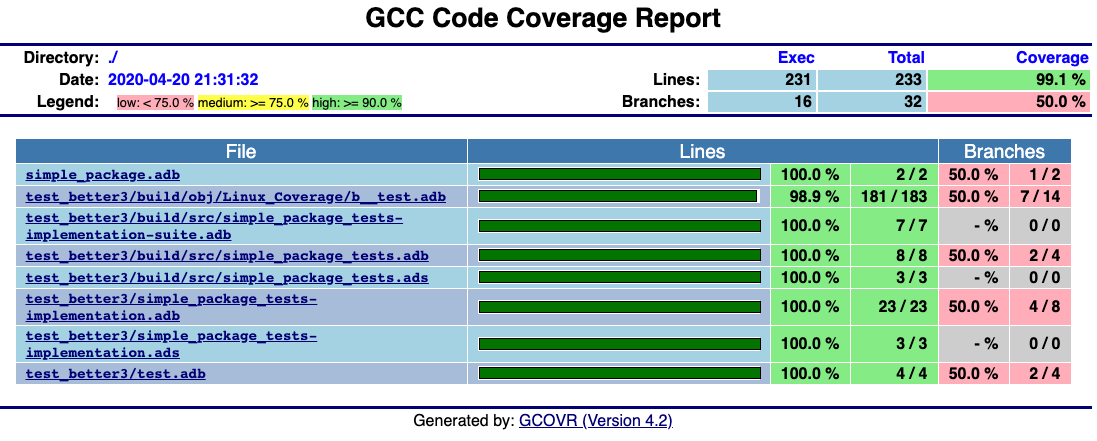
\includegraphics[width=\textwidth]{images/gcovr1.png}
\vspace{5mm} %5mm vertical space

\textit{Specific File Page:}

\vspace{5mm} %5mm vertical space
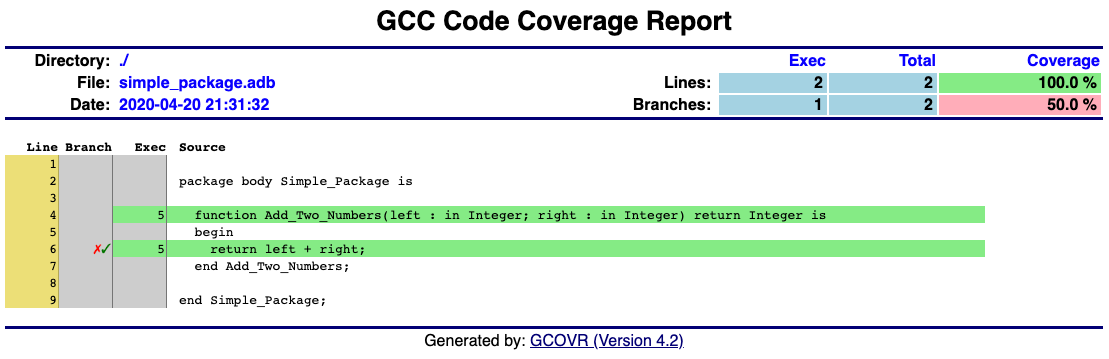
\includegraphics[width=\textwidth]{images/gcovr2.png}
\vspace{5mm} %5mm vertical space


\subsubsection{Unit Test Documentation} \label{Unit Test Documentation}

Adamant provides automatic generation of documentation for any unit test model. Currently two versions of documentation can be created: HTML, which is useful for presentation in meetings or for quick reference, and PDF (via \LaTeX), which is useful for formal documentation.\\

To build HTML documentation run:

\vspace{5mm} %5mm vertical space
\begin{minted}{text}
> redo build/html/simple_package_tests.html
\end{minted}
\vspace{5mm} %5mm vertical space

which when opened with your favorite web browser looks something like this: \\

\vspace{5mm} %5mm vertical space
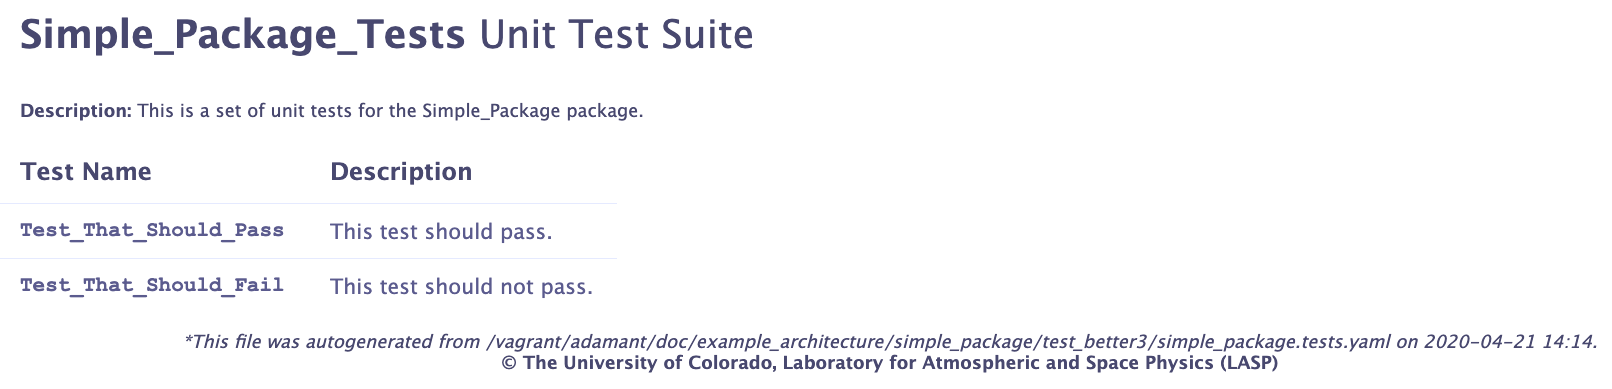
\includegraphics[width=\textwidth]{images/uthtml.png}
\vspace{5mm} %5mm vertical space

To build the PDF documentation run:

\vspace{5mm} %5mm vertical space
\begin{minted}{text}
> redo build/pdf/simple_package_tests.pdf
\end{minted}
\vspace{5mm} %5mm vertical space

Which produces a PDF output that looks like the following. \\

\noindent\makebox[\linewidth]{\rule{\textwidth}{0.4pt}}
\input{../example_architecture/simple_package/test_better3/build/tex/simple_package_tests.tex}
\noindent\makebox[\linewidth]{\rule{\textwidth}{0.4pt}}


\subsection{Object-oriented Design}

The following section introduces you to object-oriented design in Ada and the standard practices and conventions used in Adamant. In addition, we walk through how to unit test an object-oriented package.

\subsubsection{Creating an Object-oriented Package}

The previous sections discussed writing, compiling, and unit testing a simple Ada package in Adamant. The source code for Adamant heavily utilizes object-oriented design principles, where programming operations are mostly concerned with the interaction and behavior of ``objects". This section shows how to create a very simple ``class"-like entity in Ada, known as a \textit{tagged type}, which supports common object-oriented patterns such as overriding, polymorphism, dynamic dispatching, inheritance, mix-ins, etc. \\

Note that this section does not delve into the specifics of object-oriented programming in Ada. Instead it attempts to show simply what a simple \texttt{tagged type} might look like, and how unit testing it is slightly different from the example presented in the previous sections. For details on the object-oriented programming in Ada see the \href{https://en.wikibooks.org/wiki/Ada_Programming/Object_Orientation}{\textcolor{blue}{Ada Programming Wiki}} or \href{https://learn.adacore.com/courses/intro-to-ada/chapters/object_oriented_programming.html}{\textcolor{blue}{AdaCore Learn}}. \\

First let's create a directory for the package as before, and add this directory to the \textit{build path}.

\vspace{5mm} %5mm vertical space
\begin{minted}{text}
> mkdir oo_package 
> cd oo_package 
> touch .all_path  # add directory to the build path
\end{minted}
\vspace{5mm} %5mm vertical space

Below is the source code for an object-oriented tagged type that we can put in this directory:

\textit{oo\_package.ads}:

\adacodef{../example_architecture/oo_package/oo_package.ads}

\textit{oo\_package.adb}:

\adacodef{../example_architecture/oo_package/oo_package.adb}

We can see that the package contains a tagged type named \texttt{Instance}. \textit{Instance} is the standard name used for a tagged type within Adamant when a package contains a single tagged type, which is common. \\

Below the tagged type is two public subprograms, or ``primitives". These subprograms are considered primitive operations of the tagged type \texttt{Instance} because \texttt{Instance} is passed as an argument to them. Primitives are similar to ``methods" in Java or a ``member functions" in C++. The first subprogram is a procedure called \texttt{Init} which initializes the object, which is always named \texttt{self} in Adamant. The second subprogram implements an adding function similar to what was presented in the previous sections. This time, however, a private variable, \texttt{n}, stored within the tagged type record is added to the input argument instead. The variable \texttt{n} is part of the private definition of type \texttt{Instance} and thus cannot be accessed outside of the \texttt{Oo\_Package}, except within a child package, as we will see in the next section.

\subsubsection{``White-box" Unit Testing}

In this section we unit test the object-oriented package we created in the previous section. Tagged types are unique in that they act as objects that encapsolate private data members. These data members are usually not accessible to the outside world, meaning the only way to test the object-oriented package is by calling its public methods, also known as ``black-box" testing. However, using the patterns seen in this section, we also perform ``white-box" testing, allowing us the safely check the values of the private members within the object, without compromising the type safety of the deployment code by making the type definition public.

First, let's create an Adamant unit test YAML file as before in a directory called \textit{test/}.

\vspace{5mm} %5mm vertical space
\begin{minted}{text}
> mkdir test  # Make test/ within oo_package/
> cd test 
\end{minted}
\vspace{5mm} %5mm vertical space

In this directory we can create a test model file called \textit{oo\_package.tests.yaml} with the following contents:

\yamlcodef{../example_architecture/oo_package/test/oo_package.tests.yaml}

We declare two tests, one to test each of the primitive operations of our tagged type. \\

Note that within our unit tests we are not able to access the private member variable \texttt{n} within \texttt{Oo\_Package.Instance} unless we create a special ``child" package that can provide us visibility. In Ada, child packages have access the private variables and subprograms found in their parent package. Note that a child package is not the same as type inheritance, which is a distinct concept in Ada. Child packages ONLY provide a mechanism for package extension and control of private sections. \\

Let's create a child package called \texttt{Oo\_Package.Tester} that has a function that gives us visibility into the private variable \texttt{n}. Note the file and package naming conventions seen below. This pattern is required by Ada for proper compilation of a child package. \\

\textit{oo\_package-tester.ads}:

\adacodef{../example_architecture/oo_package/test/oo_package-tester.ads}

\textit{oo\_package-tester.adb}:

\adacodef{../example_architecture/oo_package/test/oo_package-tester.adb}

Excellent. We can now use this fancy new package and function in our unit tests. To write our unit tests we follow the same procedure as presented previously. First, we make the unit test templates, copy them into our test directory, and them modify them to taste. 

\vspace{5mm} %5mm vertical space
\begin{minted}{text}
> redo build/template/oo_package_tests-implementation.adb
> redo build/template/oo_package_tests-implementation.ads
> redo build/template/test.adb
> cp build/template/* .  # copy the template files into test_better/
\end{minted}
\vspace{5mm} %5mm vertical space

The unit test files with complete unit test code are shown below.

\textit{oo\_package\_tests-implementation.ads}:

\adacodef{../example_architecture/oo_package/test/oo_package_tests-implementation.ads}

\textit{oo\_package\_tests-implementation.adb}:

\adacodef{../example_architecture/oo_package/test/oo_package_tests-implementation.adb}

There are a few important differences here compared to the previous sections. First, an object of type \texttt{Oo\_Package.Instance} is declared in the record of the unit test packed record itself named \texttt{Oo}. This makes the object part of the unit test class, and thus callable from the fixtures and unit test procedures. Second, we use the \texttt{Set\_Up\_Test} fixture this time to call the \texttt{Init} method on the \texttt{Oo\_Package.Instance} object. This fixture will get called before both unit tests are run. \\

In the first unit test, all we do is call the special function we implemented in the child package \textit{oo\_package-tester.ads}, which gives us visibility into the private variable \texttt{N}. This test makes sure that \texttt{N} was initialized properly via the \texttt{Init} function. In the second unit test we call the addition function and make sure it returns the expected result. We also call the child subprogram \texttt{Get\_N} again to make sure that the internal state of the \texttt{Oo\_Package.Instance} object did not change as a result of the call to \texttt{Self.Oo.Add\_N}, which should not modify the object. \\

Everything works as expected and produces the test output:

\vspace{5mm} %5mm vertical space
\inputminted{text}{ ../example_architecture/oo_package/test/output.txt}
\vspace{5mm} %5mm vertical space

\newpage
\section{Packed Types} \label{Packed Types}

Often in embedded systems, communication protocols and access to hardware devices require specific patterns of transferred bytes and bits to properly function. However, technical differences in processors and compilers can often make code reuse difficult to achieve in a cross-platform and portable way. For instance, processors used in the design of embedded systems can be either big or little endian, depending on the chosen platform. Embedded systems often communicate with other embedded processors or end-user systems which have an endianness different from their own. If not carefully handled, these differences in endianness can be one of the largest sources of defects encountered while debugging embedded software. Besides endianness issues, the ``packed"-ness, that is, the amount of padding supplied around individual types, of a struct or array in processor memory differs based on the compiler used. The differences in endianness and ``packed"-ness can make writing portable software difficult without a layer of abstraction to handle the differences.

Adamant aims to solve these problem through the use of \textit{packed types}.  In Adamant, packed types are modeled using a YAML specification. From the specification, the following type definitions are generated:

\begin{spaceditemize}
  \item \textbf{\texttt{T}} - A big endian representation of the type. These are the most commonly seen type in Adamant.
  \item \textbf{\texttt{T\_Le}} - A little endian representation of the type. This is usually only used to communicate with little endian specific hardware.
  \item \textbf{\texttt{U}} - A \textit{native} version of the type whose bit layout has been chosen by the compiler. This is usually the most performant version of the type, but the bit layout changes based on the compiler used, and thus is not portable. This version is often used when performance is a concern, but the layout of the bits does not matter.
\end{spaceditemize}

The \texttt{T} and \texttt{T\_Le} types can be thought of as the \textit{serialized} version of the record, where the bit layout and endianness is known, no matter the compiler or processor that the code is running on. The \texttt{U} version of the type can be thought of as the \textit{native} version of the type, which has been optimized by the compiler for the target processor. For each of the types above Adamant also provides facilities to validate that the values in the type are within range, pretty print the type, check the value of the type during testing via assertions, and produce HTML and PDF documentation for the type. These features are discussed in the following subsections.

\subsection{Packed Records} \label{Packed Records}

Using packed records is the preferred method of declaring data types in Adamant. A packed record is a structure-like datatype which can contain an arbitrary number of fields of any type, including arrays, packed arrays, or even other packed records.

To define a packed record, a developer should create a YAML model file of the form \textit{name.record.yaml}, where \textit{name} is the desired name of the packed record. Let's create a record with the following fields:

\begin{spaceditemize}
  \item \textbf{\texttt{Value\_1}} - A five bit modular type that wraps around at 32.
  \item \textbf{\texttt{Value\_2}} - A 3 bit signed integer type with a valid range from -3 to 2.
  \item \textbf{\texttt{Value\_3}} - An 8-bit enumeration type with valid states: Red, Green, Blue, Purple, Pink, and Chartreuse
  \item \textbf{\texttt{Value\_4}} - A 32-bit floating point type.
\end{spaceditemize}

Below is the example packed record definition called \textit{example\_record}, stored in a file called \textit{example\_record.record.yaml}:

\yamlcodef{../example_architecture/example_record.record.yaml}

This YAML model file above contains comments explaining whether or not each field is optional or required. The main portion of the model is the packed record \textit{fields} which require a \textit{name}, \textit{type}, and \textit{format} specification. The type of the field can be any Ada type, including arrays, records, enumerations, packed arrays, or other packed records. The \textit{format} field is where a developer can describe out how the field is represented in memory in its packed form. This field takes an enumeration of the form \textit{U}, \textit{I}, \textit{F} or \textit{E} (for unsigned, signed, floating point, or enumeration) followed by the number of bits used to represent it. A table of example memory representations is laid out below:

\captionof{table}{Example Packed Record Format Specifications}
\begin{xltabular}{\textwidth}{ | l | X | }
  \hline
  \textbf{Format} & \textbf{Description} \\ \hline
    \texttt{U8} & Unsigned 8-bit integer \\ \hline
    \texttt{I16} & Signed 16-bit integer \\ \hline
    \texttt{U1} & Unsigned single bit \\ \hline
    \texttt{I13} & Signed 13-bit integer \\ \hline
    \texttt{F32} & 32-bit floating point value \\ \hline
    \texttt{F64} & 64-bit floating point value \\ \hline
    \texttt{E3} & 3-bit enumeration type \\ \hline
    \texttt{U8x32} & 32-bytes of unsigned integers (often used for arrays) \\ \hline
    \texttt{E5x10} & an array of ten 5-bit enumerations \\ \hline
\end{xltabular}

Ada uses the \textit{format} specification to understand the number of bits taken up by the type. If the number of bits specified in the representation field is not compatible with the type specified in the type field, the Ada compiler will warn or error, telling the user to fix the inconsistency. The enumeration portion of the \textit{format} is needed is to make the record visible to a ground system, such as Hydra. Adamant currently supports the display of many representations in Hydra including all signed and unsigned integers from 1 to 64 bits and floating point numbers of 32 and 64 precision and enumeration types. There is no support in Adamant or Hydra to display values with representations over 64 bits in length. The record should be further divided or an array \textit{format} should be used in this case. Note that an entire record's length must end on a 1 byte (8-bit) boundary, or a error message will be produced. Add additional fields of pad bytes to make the total length of the record end on an 8-bit boundary.

\subsubsection{Packed Record Ada Specification} \label{Packed Record Ada Specification}

The \textit{example\_record.record.yaml} file produces a single Ada specification file which declares a package containing the packed and unpacked representations of the record. The file can be generated and compiled by running the following command from the same directory as \textit{example\_record.record.yaml}:

\vspace{5mm} %5mm vertical space
\begin{minted}{text}
> cd to/dir/with/example_record
> redo build/obj/Linux/example_record.o
\end{minted}
\vspace{5mm} %5mm vertical space

Two source code files are autocoded: \textit{build/src/example\_record.ads} and \textit{build/src/example\_record.adb}. Below is the specification file, \textit{build/src/example\_record.ads}.

\adacodef{../example_architecture/build/src/example_record.ads}

A record is produced with 4 fields as expected. The \texttt{U} type will respect the Ada \textit{type} given in the YAML file, and any range or default value associated with it. The representation of this type on disk is completely up to the compiler. The unpacked type should be used whenever the type is used in heavy calculations, since the compiler will be able to optimize the program for speed instead of spending time worrying about storage space and endianness. If the representation or size of the type is of concern, like when sending the data through a connector or to a different processing unit, the \texttt{T} type should be used. This is a specialization of the \texttt{U} type which specifies exactly how the record should be laid out in memory. The size of each field is calculated, and a big endian representation is requested. \\ 

Some examples of how to use the specification are presented in the following two sections.

\subsubsection{Packed Record Type Conversion} \label{Packed Record Type Conversion}

Converting a record between the \texttt{T} and \texttt{U} types (and vise-versa) is trivial since the \texttt{T} type is a derived type of \texttt{U}. Converting between the two is as simple as using an explicit type conversion, ie:

\adacodef{../example_architecture/record_conversion/main.adb}

\subsubsection{Packed Record Serialization} \label{Packed Record Serialization}

Also included in the specification is the \texttt{Serialization} package which can be used to convert the packed record to and from an array of bytes, which is a very common operation in embedded systems. Here is an example:

\adacodef{../example_architecture/record_serialization/main.adb}

Note also that with every packed record there are a series of \texttt{Serialized\_Length} subprograms. These subprograms allow the user to determine the length of a type (in bytes). While the length of the packed record presented in this section is static, meaning the function always returns the same value, variable length packed records return different values based on the type's content. See Section \ref{Variable Length Packed Records} for more details.

\subsubsection{Packed Record Validation} \label{Packed Record Validation}

Using the serialization and deserialization functions shown in the previous section can be error prone. Consider the field in our record \texttt{Value\_2}, which only has a valid integer range between -2 and 3. It is possible that when calling the deserialization function \texttt{From\_Byte\_Array}, the incoming byte array might contain a bit representation the puts the \texttt{Value\_2} field out of range, ie. 5. The call to \texttt{From\_Byte\_Array} will not fail, but any subsequent operation using the \texttt{packed\_Type} variable will fail with an Ada constraint error, due the range check failing on \texttt{Value\_2}. \\

Adamant packed records have a method for mitigating this using an autocoded child package which performs validation on the type. To build the validation child package run the following:

\vspace{5mm} %5mm vertical space
\begin{minted}{text}
> redo build/obj/Linux/example_record-validation.o
\end{minted}
\vspace{5mm} %5mm vertical space

This generates the source files \textit{build/src/example\_record-validation.ads} and \textit{build/src/example\_record-validation.adb}. The autocoded specification is shown below.

\adacodef{../example_architecture/build/src/example_record-validation.ads}

Note that a \texttt{Valid} function which returns a \texttt{Boolean} is available to validate each version of the packed record. These functions can be called to determine if the type is within range, and thus safe to use, before using the type elsewhere in the system. The Adamant component autocoder uses the feature extensively to validate incoming commands and parameters prior to their use within user code.\\

Below is an example of using this package.

\adacodef{../example_architecture/record_validation/main.adb}

which, when run, produces the output:

\vspace{5mm} %5mm vertical space
\inputminted{text}{../example_architecture/record_validation/output.txt}
\vspace{5mm} %5mm vertical space

which shows that a byte value of 255 is out of range for the enumeration type used for \texttt{Value\_3}. \\

Note that Adamant currently struggles to support validation for certain Ada types including \texttt{System.Address} and all access types. The inclusion of these in packed records is rare in practice so this does not pose a critical issue. If the validation autocode for a certain field does not compile you have two options: 1) Don't use the autocoded package and instead hand-code your own or 2) If you know that the type will always be valid then use the \texttt{Skip\_Validation} field modifier to specify that you want the autocoder to skip generating validation code for that field. Below is a packed record \textit{memory\_region.record.yaml} that uses \texttt{Skip\_Validation} to avoid validating a troublesome address type.

\yamlcodef{../../src/types/memory/32bit/memory_region.record.yaml}

If not specified the \texttt{Skip\_Validation} defaults to \texttt{False}. The unusual \texttt{Byte\_Image} modifier is also seen in this YAML file. See the Section \ref{Packed Record String Representation} for more details.

\subsubsection{Packed Record String Representation} \label{Packed Record String Representation}

During testing, it is often nice to print the value of a complex datatype in a human readable form. Adamant has the ability to generate human readable string representations for packed records. The string representation code for the \texttt{example\_record} is included in two files, a specification \textit{build/src/example\_record-representation.ads} and \textit{build/src/example\_record-representation.adb} which can be generated and compiled using the following commands: 

\vspace{5mm} %5mm vertical space
\begin{minted}{text}
> redo build/obj/Linux/example_record-representation.o
\end{minted}
\vspace{5mm} %5mm vertical space

This generates the source files \textit{build/src/example\_record-representation.ads} and \textit{build/src/example\_record-representation.adb}. The autocoded specification is shown below.

\adacodef{../example_architecture/build/src/example_record-representation.ads}

There are many subprograms provided, but the most commonly used are \texttt{To\_Byte\_String}, \texttt{Image}, and \texttt{To\_Tuple\_String}. The first \texttt{To\_Byte\_String} function returns a string that shows the bytes that make up the packed record in hex. The second \texttt{Image} functions returns the most human readable representation of the packed record, printing each field name following by its value on a separate line. The \texttt{To\_Tuple\_String} is useful for logging, as the entire record is always printed, comma separated, on a single line. \\

Below is an example of using the package.

\adacodef{../example_architecture/record_representation/main.adb}

which, when run, produces the output:

\vspace{5mm} %5mm vertical space
\inputminted{text}{../example_architecture/record_representation/output.txt}
\vspace{5mm} %5mm vertical space

Note that Adamant currently struggles to support pretty print strings for certain Ada types including \texttt{System.Address} and all access types. The inclusion of these in packed records is rare in practice so this does not pose a critical issue. If the string representation autocode for a certain field type is not to your liking, or does not compile you have two options: 1) Don't use the autocoded package and instead hand-code your own, see the \texttt{Sys\_Time} type for an example of this, or 2) Use the \texttt{Byte\_Image} field modifier to specify that you want the representation of the type to simply be an array of hex bytes. Since any type can be represented by its underlying machine byte values, option 2 will always compile, but may not be as human readable. Below is a packed record \textit{memory\_region.record.yaml} that uses \texttt{Byte\_Image} to display a troublesome address type.

\yamlcodef{../../src/types/memory/32bit/memory_region.record.yaml}

If not specified the \texttt{Byte\_Image} defaults to \texttt{False}. The unusual \texttt{Skip\_Validation} modifier is also seen in this YAML file. See the Section \ref{Packed Record Validation} for more details.

\subsubsection{Packed Record Unit Test Assertions}\label{Packed Record Unit Test Assertions}

Adamant also provides an assertion package for each packed record. The assertion package is useful during unit testing, as it allows you to compare two packed types. If the packed types do not meet the comparison criteria, then a human readable error message is printed. To build the assertion package run.

\vspace{5mm} %5mm vertical space
\begin{minted}{text}
> redo build/obj/Linux/example_record-assertion.o
\end{minted}
\vspace{5mm} %5mm vertical space

The \textit{build/src/example\_record-assertion.ads} and \textit{build/src/example\_record-assertion.adb} files are autocoded. The specification is shown below.

\adacodef{../example_architecture/build/src/example_record-assertion.ads}

The package uses the Adamant \texttt{Smart\_Assert} package and can be used as follows:

\adacodef{../example_architecture/record_assertion/main.adb}

which, when run, produces the output:

\vspace{5mm} %5mm vertical space
\inputminted{text}{../example_architecture/record_assertion/output.txt}
\vspace{5mm} %5mm vertical space

\subsubsection{Packed Record Documentation}

Adamant provides automatic generation of documentation for any packed record definition. Currently two versions of documentation can be created: HTML, which is useful for presentation in meetings or for quick reference, and PDF (via \LaTeX), which is useful for formal documentation.\\

To build HTML documentation run:

\vspace{5mm} %5mm vertical space
\begin{minted}{text}
> redo build/html/example_record.html
\end{minted}
\vspace{5mm} %5mm vertical space

which when opened with your favorite web browser looks something like this: \\

\vspace{5mm} %5mm vertical space
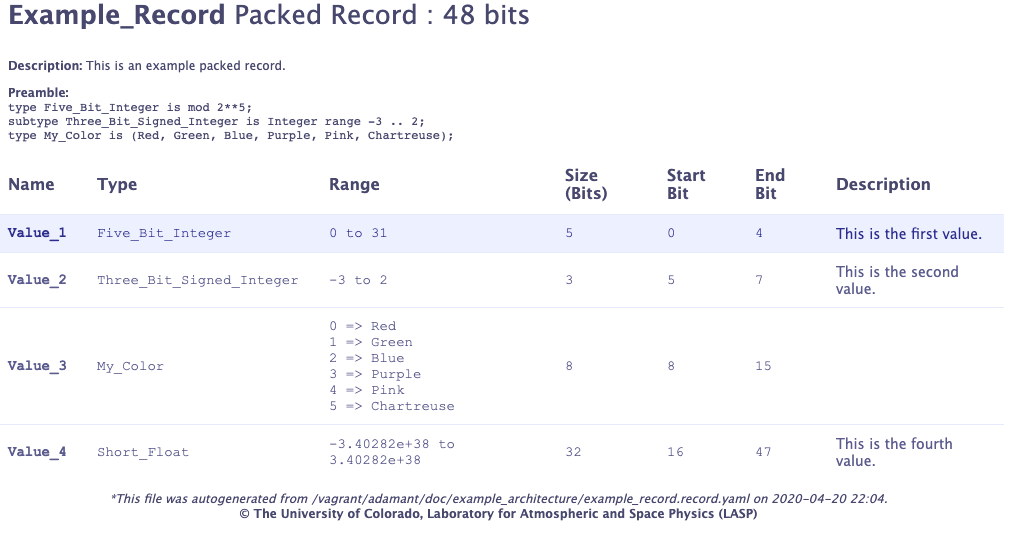
\includegraphics[width=\textwidth]{images/recordhtml.png}
\vspace{5mm} %5mm vertical space

To build the PDF documentation run:

\vspace{5mm} %5mm vertical space
\begin{minted}{text}
> redo build/pdf/example_record.pdf
\end{minted}
\vspace{5mm} %5mm vertical space

Which produces a PDF output that looks like the following. \\

\noindent\makebox[\linewidth]{\rule{\textwidth}{0.4pt}}
\input{../example_architecture/build/tex/example_record.tex}
\noindent\makebox[\linewidth]{\rule{\textwidth}{0.4pt}}

\subsubsection{Packed Record Python Class} \label{Packed Record Python Class}

For each packed type, Adamant provides a python class which supplies analogous operations to the Ada serialization, representation, and assertion packages presented in the previous sections. For space-based applications, these python classes are meant as ``ground" tools, or tools which assist with some task related to the deployed embedded system such as testing, parsing data, sending commands, etc. See Section \ref{Ground Tools} for more details. To build the python class for a record run:

\vspace{5mm} %5mm vertical space
\begin{minted}{text}
> redo build/py/example_record.py
\end{minted}
\vspace{5mm} %5mm vertical space

The resulting autocode is shown below:

\pythoncodef{../example_architecture/build/py/example_record.py}

The python classes use the \texttt{bitstring} python module which allows easily manipulation of an object that acts like an array of bits. The python class contains the following methods - note that some of the methods below are actually implemented in the python packed type base class \texttt{PackedTypeBase}, from which the autocode inherits:

\vspace{5mm} %5mm vertical space
\begin{spaceditemize}
  \item \textbf{\texttt{\_\_init\_\_}} - Create a packed record. The record field values are optional upon initialization, and will be set to the default or \texttt{None} if there is no default. During initialization, the class performs extensive type checking of the record fields to make sure that their values adhere to ranges of the equivalent Ada types.
  \item \textbf{\texttt{\_\_eq\_\_}} - Compares two packed records for equality.
  \item \textbf{\texttt{serialized\_length}} - Equivalent to the Ada \texttt{Serialized\_Length} function, returns the length of the packed type.
  \item \textbf{\texttt{to\_byte\_array} and \texttt{from\_byte\_array}} - Equivalent to the Ada serialization/deserialization functions \texttt{Serialization.To\_Byte\_Array} and \texttt{Serialization.From\_Byte\_Array}; converts the python class to a serialized byte array whose bits correspond to the layout of the packed big-endian type (\texttt{T}) in Ada, or takes a byte array of this form an turns it into a python class.
  \item \textbf{\texttt{create\_from\_byte\_array}} - Creates a new packed record object from a serialized byte array.
  \item \textbf{\texttt{\_\_repr\_\_}, \texttt{\_\_str\_\_} and \texttt{to\_string}} - Equivalent to the Ada \texttt{Representation.Image} function; creates a human readable string version of the packed record.
  \item \textbf{\texttt{to\_tuple\_string}} - Equivalent to the Ada \texttt{Representation.To\_Tuple\_String} function; creates a log-friendly string of the packed record.
\end{spaceditemize}
\vspace{5mm} %5mm vertical space

An example of how this class can be used is shown below in a file called \textit{test.py}:

\pythoncodef{../example_architecture/record_py/test.py}

Note the call at the top of the script to \texttt{pydep.build\_py\_deps()}. This Adamant python module does two useful things: 1) it searches the python program for any autocoded dependencies and uses \texttt{redo} to build them and 2) adds any autocoded dependencies automatically to the \texttt{PYTHONPATH} so they can be imported without error. It is important to run this function as the first line of any Adamant python script that will use autocoded python classes. \\

The script can be run with the command:

\vspace{5mm} %5mm vertical space
\begin{minted}{text}
> python test.py
\end{minted}
\vspace{5mm} %5mm vertical space

and produces the following output:

\vspace{5mm} %5mm vertical space
\inputminted{text}{../example_architecture/record_py/output.txt}
\vspace{5mm} %5mm vertical space

Python classes can also be autogenerated for variable-length packed records and packed arrays, presented in the following sections.

\subsubsection{Packed Record MATLAB Class} \label{Packed Record MATLAB Class}

For each packed type, Adamant provides a MATLAB class which supplies analogous operations to the Ada and python serialization, representation, and assertion packages presented in the previous sections. For space-based applications, these MATLAB classes are meant as ``ground" tools, or tools which assist with some task related to the deployed embedded system such as testing, parsing data, sending commands, etc. See Section \ref{Ground Tools} for more details. To build the MATLAB class for a record run:

\vspace{5mm} %5mm vertical space
\begin{minted}{text}
> redo build/m/Example_Record.m
\end{minted}
\vspace{5mm} %5mm vertical space

The resulting autocode is shown below:

\matlabcodef{../example_architecture/build/m/Example_Record.m}

The MATLAB classes use the \texttt{Bit\_Array} MATLAB class, found in \textit{gnd/matlab/Bit\_Array.m}, which allows easily manipulation of an object that acts like an array of bits. Each autocoded MATLAB class uses \texttt{Bit\_Array} to provide the following methods:

\vspace{5mm} %5mm vertical space
\begin{spaceditemize}
  \item \textbf{\texttt{Example\_Record}} - The constructor used to create a packed record object. The record field values are optional required initialization. The class performs extensive type checking of the record fields to make sure that their values adhere to ranges of the equivalent Ada types, where possible.
  \item \textbf{\texttt{eq}} - Compares two packed records for equality.
  \item \textbf{\texttt{ne}} - Opposite of \texttt{eq}.
  \item \textbf{\texttt{serialized\_length}} - Equivalent to the Ada \texttt{Serialized\_Length} function, returns the length of the packed type.
  \item \textbf{\texttt{to\_byte\_array} and \texttt{from\_byte\_array}} - Equivalent to the Ada serialization/deserialization functions \texttt{Serialization.To\_Byte\_Array} and \texttt{Serialization.From\_Byte\_Array}; converts the MATLAB class to a serialized byte array whose bits correspond to the layout of the packed big-endian type (\texttt{T}) in Ada, or takes a byte array of this form an turns it into a MATLAB class.
  \item \textbf{\texttt{create\_from\_byte\_array}} - Creates a new packed record object from a serialized byte array.
  \item \textbf{\texttt{create\_empty}} - Creates a new packed record object where the default values of all fields is zero, or the lowest legal value where zero is not allowed.
  \item \textbf{\texttt{to\_string}} - Equivalent to the Ada \texttt{Representation.Image} function; creates a human readable string version of the packed record.
  \item \textbf{\texttt{to\_tuple\_string}} - Equivalent to the Ada \texttt{Representation.To\_Tuple\_String} function; creates a log-friendly string of the packed record.
\end{spaceditemize}
\vspace{5mm} %5mm vertical space

An example of how this class can be used is shown below in a file called \textit{test.m}:

\matlabcodef{../example_architecture/record_m/test.m}

The script can be run from the MATLAB command prompt:

\vspace{5mm} %5mm vertical space
\begin{minted}{text}
>> test
create and disp example record:
  Example_Record with properties:

                          Value_1: 2
                          Value_2: -1
                          Value_3: 1
                          Value_4: 0.5
                             size: 48
                    size_in_bytes: 6
    min_serialized_length_in_bits: 48
    max_serialized_length_in_bits: 48
            min_serialized_length: 6
            max_serialized_length: 6
                       num_fields: 4
(Value_1 = 2, Value_2 = -1, Value_3 = 1, Value_4 = 0.5)
[17 01 3f 00 00 00]
Value_1 : Five_Bit_Integer = 2
Value_2 : Three_Bit_Signed_Integer = -1
Value_3 : My_Color = 1
Value_4 : Short_Float = 0.5
[17 01 3f 00 00 00]
done.
\end{minted}
\vspace{5mm} %5mm vertical space

MATLAB classes can also be autogenerated for variable-length packed records and packed arrays, presented in the following sections.

Note that it is up to the user to make sure their MATLAB path is configured to include the appropriate directories for their program. Sometimes it is convenient to have all autocoded MATLAB copied to a single directory. Adamant provides some scripts to achieve this in \textit{gnd/matlab/build\_all\_matlab\_autocode.sh} and \textit{gnd/matlab/copy\_all\_matlab\_autocode.sh}.

\subsubsection{Variable Length Packed Records} \label{Variable Length Packed Records}

The packed types that have been presented so far are all static in length. To be more specific, when these types are put onto an Adamant queue, they always take up the same amount of memory. For memory efficiency, Adamant also supports variable length packed records. In particular these records have two main features that are common in many communication protocols:

\vspace{5mm} %5mm vertical space
\begin{spaceditemize}
  \item \textbf{\texttt{Array of Values}} - An array of values, often bytes, that are usually filled with multi-purpose data
  \item \textbf{\texttt{Length}} - A number, often in a protocol header, which indicates how many values in the array are valid and currently in use
\end{spaceditemize}
\vspace{5mm} %5mm vertical space

One common protocol type used in space-based applications that follows this paradigm is a CCSDS packet, which contains an array of data bytes, whose length is specified by a specific value in the CCSDS header. Adamant uses variable length fields for many common types including commands, events, parameters, faults, and packets. Find these definitions in the \texttt{src/types} directory to explore good examples of variable length packed records. \\

Adamant variable length records offer an advantage when they are put onto queues. When enqueueing a variable length type, only the valid portion of the data is stored on the queue, not the maximum size of the type. So for instance, if the maximum size of a variable length packed record is 1000 bytes, but only 12 bytes are being specified as ``used" by the length field, then only 12 bytes (plus some overhead) will be used on an Adamant queue to store the type. Note that when declaring a variable length type on the stack, the maximum size of the type will still be allocated. Care must still be taken in defining a reasonably sized maximum array length so as to not overflow the stack. \\

Adamant variable length packed records are optimized for speed, at the cost of flexibility. As a result they must adhere to the following constraints:

\vspace{5mm} %5mm vertical space
\begin{spacedenumerate}
  \item There may only be a single variable length field, ie. \textit{array of values}, in a packed record.
  \item The variable length field of the record must be the last field specified in the packed record.
  \item All fields in a variable length record must be byte aligned. 
\end{spacedenumerate}
\vspace{5mm} %5mm vertical space

Note that item 3 can be overcome by encapsulating any non-byte aligned fields in their own packed record (which as a whole must be byte aligned), and then including that packed record as the type for a field within variable length packed record. See the CCSDS Primary Header definition within Adamant for an example of this. \\

To define a variable length packed record we introduce a new specification \texttt{variable\_length} and \texttt{variable\_length\_offset} to the packed record YAML definition. Below is a simple example:

\yamlcodef{../example_architecture/example_variable_record.record.yaml}

The \texttt{variable\_length} specification in the \texttt{Buffer} field indicates that 1) the \texttt{Buffer} field is of variable length and 2) that the \texttt{Length} field will be used to determine that length during runtime. The \texttt{variable\_length\_offset} field is a signed integer that will be added to the \texttt{Length} field during runtime to modify how the value is treated. For most sane protocols this value will always be 0, which is the default, and need not be specified. Some protocols, notably CCSDS, deviates from this and requires a value of 1 be specified for the \texttt{variable\_length\_offset}. \\

Note that the variable length field may be any type as long as it is an array. This can include arrays of non-byte aligned elements (so long as the whole array is byte aligned), arrays with elements larger than a single byte (such as a float), packed arrays (discussed in the previous sections), and even packed arrays whose element type is a packed record. The length field always specifies the number of used elements in the array in units of the array element type. It does not specify the number of valid bytes that are used unless, of course, the array element type is specifically a byte. \\

For the most part, variable length packed records have the same facilities available to them as their non-variable length counterparts including a serialization package, validation package, representation package, and an assertion package. There are subtle differences in the subprogram interface for some of the utilities, so see the specification of the autogenerated code to make sure that you are making the right calls, and providing proper error handling. In particular, serialization and deserialization of a variable length packed record can fail if the length field is larger than the array it is describing. In this case, any serialization and deserialization calls return a status to the caller that must be handled appropriately. Similarly, for assertions, there exists an assertion call to compare an entire variable length record against another up to the maximum size, and another which only compares the ``used" variable length data, and ignores the data beyond.

The mechanism for determining a variable length record's length is the autocoded \texttt{Serialized\_Length} subprograms provided in the specification. These subprograms allow the user to determine the length of a type (in bytes). While the length of most packed records are static, meaning the function will always return the same value, variable length packed records will return different values based on the type's content, ie. the \texttt{variable\_length} field. These \texttt{Serialized\_Length} subprograms are important because they are required by all generic packages within adamant that deal with variable length packed records, including Adamant's variable queue package used for component queues, see Section \ref{The Component Queue}.

\subsection{Packed Arrays}

Packed arrays are similar to their packed record counterparts, and contain all of the features presented in the previous packed record sections. Specifying a packed arrays requires providing an element type and a length. The element type may be of any type including packed arrays, packed records, or types that don't end on a byte boundary. The resulting autocoded packed type will be of static length and of the type provided. The size of the array in memory will be packed such that it is the size of the format specified (in bits) multiplied by the length.

One useful utility of packed arrays might be to declare an array of 10-bit items that is packed tight with no padding. This is the idea we will use for our example. We want to declare an array of 10-bit integers with a valid range between 0 and 999 that is 8 elements long. Because the array is made up of 10-bit numbers, the packed version of the array should only take up 10-bytes in memory. Note, that some versions of the Ada compiler will require packed arrays to end on a 4-byte boundary. A compiler error will be thrown in this case, and you may have to modify your packed array YAML to comply.

To define a packed array, a developer should create a YAML model file of the form \textit{name.array.yaml}, where \textit{name} is the desired name of the packed array. Below is the example packed array definition called \textit{example\_array}, stored in a file called \textit{example\_array.array.yaml}:

\yamlcodef{../example_architecture/example_array.array.yaml}

This YAML model file above contains comments explaining whether or not each field is optional or required. The main portion of the model is the packed array \textit{type}, \textit{length}, and \textit{format} specification. The type of the field can be any Ada type, including arrays, records, enumerations, packed records, or other packed arrays. The \textit{format} field is where a developer can describe out how the field will be represented in memory in its packed form, and is identical to the format specification for packed records. See the previous sections for more details on \textit{format}. The \textit{length} field specifies how many elements the packed array contains. Unconstrained packed arrays are not currently supported in Adamant.

\subsubsection{Packed Array Ada Specification}

The \textit{example\_array.array.yaml} file produces a single Ada specification file which declares a package containing the packed and unpacked representations of the array. The file can be generated and compiled by running the following command from the same directory as \textit{example\_array.array.yaml}:

\vspace{5mm} %5mm vertical space
\begin{minted}{text}
> cd to/dir/with/example_array
> redo build/obj/Linux/example_array.o
\end{minted}
\vspace{5mm} %5mm vertical space

This will generate the source files \textit{build/src/example\_array.ads} and \textit{build/src/example\_array.adb}. The autocoded specification is shown below.

\adacodef{../example_architecture/build/src/example_array.ads}

An array is produced with the specifications we described. The \texttt{U} type will respect the Ada \textit{type} given in the YAML file, and any range associated with it. The representation of this type on disk is completely up to the compiler. The unpacked type should be used whenever the type is used in heavy calculations, since the compiler will be able to optimize the program for speed instead of spending time worrying about storage space and endianness. If the representation or size of the type is of concern, like when sending the data through a connector or to a different processing unit, the \texttt{T} type should be used. This is a specialization of the \texttt{U} type which specifies exactly how the array should be laid out in memory. The size of each field is calculated, and a big endian representation is requested.

\subsubsection{Packed Array Type Conversion}

Packed array type conversion is similar to packed record type conversion. See Section \ref{Packed Record Type Conversion} for details.

\subsubsection{Packed Array Serialization}

Packed array serialization is similar to packed record serialization. See Section \ref{Packed Record Serialization} for details.

\subsubsection{Packed Array Validation}

Packed array validation is similar to packed record validation. See Section \ref{Packed Record Validation} for details.

\subsubsection{Packed Array String Representation}

During testing, it is often nice to print the value of a complex datatype in a human readable form. Adamant has the ability to generate human readable string representations for packed arrays. The string representation code for the \texttt{example\_array} is included in two files, a specification \textit{example\_array-representation.ads} and \textit{example\_array-representation.adb} which can be generated and compiled using the following commands: 

\vspace{5mm} %5mm vertical space
\begin{minted}{text}
> redo build/obj/Linux/example_array-representation.o
\end{minted}
\vspace{5mm} %5mm vertical space

This generates the source files \textit{build/src/example\_array-representation.ads} and \textit{build/src/example\_array-representation.adb}. The autocoded specification is shown below.

\adacodef{../example_architecture/build/src/example_array-representation.ads}

There are many subprograms provided, but the most commonly used are \texttt{To\_Byte\_String}, \texttt{Image}, and \texttt{To\_Tuple\_String}. The first \texttt{To\_Byte\_String} function returns a string that shows the bytes that make up the packed array in hex. The second \texttt{Image} functions returns the most human readable representation of the packed array, printing each element name following by its value on a separate line. The \texttt{To\_Tuple\_String} is useful for logging, as the entire array is always be printed, comma separated, on a single line. \\

Below is an example of using the package.

\adacodef{../example_architecture/array_representation/main.adb}

which, when run, produces the output:

\vspace{5mm} %5mm vertical space
\inputminted{text}{../example_architecture/array_representation/output.txt}
\vspace{5mm} %5mm vertical space

Note that Adamant currently struggles to support pretty print strings for certain Ada types including \texttt{System.Address} and all access types. The inclusion of these in packed arrays is rare in practice so this does not pose a critical issue. If the string representation autocode for an element type is not to your liking, or does not compile you have two options: 1) Don't use the autocoded package and instead hand-code your own or 2) Use the \texttt{Byte\_Image} field modifier to specify that you want the representation of the type to simply be an array of hex bytes. Since any type can be represented by its underlying machine byte values, option 2 will always compile, but may not be as human readable. See Section \ref{Packed Record String Representation} for an example of using this modifier with packed records. 

\subsubsection{Packed Array Unit Test Assertions}

Packed array unit test assertions are similar to packed record unit test assertions. See Section \ref{Packed Record Unit Test Assertions} for details.

\subsubsection{Packed Array Documentation}

Adamant provides automatic generation of documentation for any packed array definition. Currently two versions of documentation can be created: HTML, which is useful for presentation in meetings or for quick reference, and PDF (via \LaTeX), which is useful for formal documentation.\\

To build HTML documentation run:

\vspace{5mm} %5mm vertical space
\begin{minted}{text}
> redo build/html/example_array.html
\end{minted}
\vspace{5mm} %5mm vertical space

which when opened with your favorite web browser looks something like this:

\vspace{5mm} %5mm vertical space
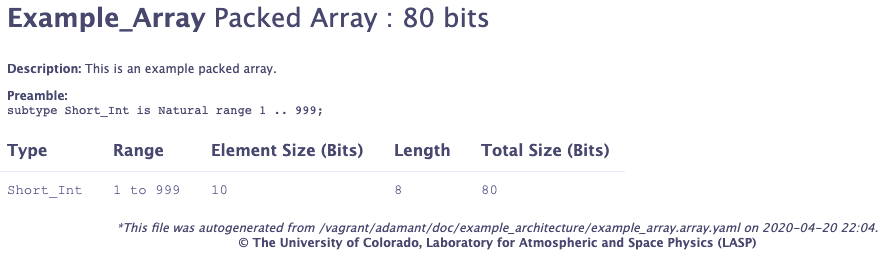
\includegraphics[width=\textwidth]{images/arrayhtml.png}
\vspace{5mm} %5mm vertical space

To build the PDF documentation run:

\vspace{5mm} %5mm vertical space
\begin{minted}{text}
> redo build/pdf/example_array.pdf
\end{minted}
\vspace{5mm} %5mm vertical space

Which produces a PDF output that looks like the following. \\

\noindent\makebox[\linewidth]{\rule{\textwidth}{0.4pt}}
\input{../example_architecture/build/tex/example_array.tex}
\noindent\makebox[\linewidth]{\rule{\textwidth}{0.4pt}}

\subsubsection{Packed Array Python Class}

Packed array python classes are similar to packed record python classes. See Section \ref{Packed Record Python Class} for details.

\subsubsection{Packed Array MATLAB Class}

Packed array MATLAB classes are similar to packed record MATLAB classes. See Section \ref{Packed Record MATLAB Class} for details.

\subsection{Enumerations}

As seen the in the previous sections, Ada enumeration types can be used in both packed records and packed arrays. Adamant also provides a mechanism to model enumerations in YAML, which can be used to autocode enumerations. These autocoded enumerations themselves are not packed types, but can easily be included in packed records as field types or as the element type within a packed array. The benefit to modeling an enumeration is that Adamant can provide autocoded assertion packages, representation packages, and documentation. Enumeration modeling should be used for enumerations that will be widely used, such as a protocol header flag, or those that are important and require extensive documentation, such as a system mode state. \\

In adamant, enumerations are modeled in suites, so many enumeration types can be described in the same YAML file. To create and enumeration suite called \textit{example\_enums}, we can write a file called \textit{example\_enums.enums.yaml}:

\yamlcodef{../example_architecture/example_enums.enums.yaml}

This YAML model file above contains comments explaining whether or not each field is optional or required. Two enumerations are described in this file: \texttt{First\_Enum} and \texttt{Second\_Enum} both of which have different states, also called literals. For each enumeration and each literal a description can be provided. An integral value can be assigned to the literal if necessary. If unspecified, Adamant assigns the lowest possible remaining unique positive integer (or zero) to each literal.

\subsubsection{Enumeration Specification}

The \textit{example\_enums.enums.yaml} file produces a single Ada specification file which declares a package containing the enumeration definitions. The file can be generated and compiled by running the following command from the same directory as \textit{example\_enums.enums.yaml}:

\vspace{5mm} %5mm vertical space
\begin{minted}{text}
> cd to/dir/with/example_enums
> redo build/obj/Linux/example_enums.o
\end{minted}
\vspace{5mm} %5mm vertical space

Below is the specification file produced, \textit{build/src/example\_enums.ads}.

\adacodef{../example_architecture/build/src/example_enums.ads}

A package is produced with two internal packages named \texttt{First\_Enum} and \texttt{Second\_Enum} which both define an enumerations named \texttt{E} that describe the literals expressed in the YAML. Note that values are assigned to each literal explicitly. If literal values are left unspecified in the YAML file, Adamant assigns the lowest possible remaining unique positive integer (or zero) to each literal, as can be seen in the \texttt{First\_Enum} package.

\subsubsection{Enumeration String Representation}

During testing, it is often nice to print the value of an enumeration in a human readable form. Adamant has the ability to generate human readable string representations for enumerations. The string representation code for the \texttt{example\_enums} is included in two files, a specification \textit{build/src/example\_enums-representation.ads} and \textit{build/src/example\_enums-representation.adb} which can be generated and compiled using the following commands: 

\vspace{5mm} %5mm vertical space
\begin{minted}{text}
> redo build/obj/Linux/example_enums-representation.o
\end{minted}
\vspace{5mm} %5mm vertical space

This generates the source files \textit{build/src/example\_enums-representation.ads} and \textit{build/src/example\_enums-representation.adb}. The autocoded specification is shown below.

\adacodef{../example_architecture/build/src/example_enums-representation.ads}

There are many subprograms provided, but the most commonly used are the \texttt{*\_Image} and the \texttt{*\_To\_Tuple\_String}. Both are pretty similar for enumerations, and the differences can be seen in the example program below.

\adacodef{../example_architecture/enum_representation/main.adb}

which, when run, produces the output:

\vspace{5mm} %5mm vertical space
\inputminted{text}{../example_architecture/enum_representation/output.txt}
\vspace{5mm} %5mm vertical space

\subsubsection{Enumeration Unit Test Assertions}

Adamant also provides an assertion package for each enumeration suite. The assertion package is useful during unit testing, as it allows you to compare two enumerations. If the enumerations do not meet the comparison criteria, then a human readable error message is printed. To build the assertion package run.

\vspace{5mm} %5mm vertical space
\begin{minted}{text}
> redo build/obj/Linux/example_enums-assertion.o
\end{minted}
\vspace{5mm} %5mm vertical space

This generates the source files \textit{build/src/example\_enums-assertion.ads} and \textit{build/src/example\_enums-assertion.adb}. The autocoded specification is shown below.

\adacodef{../example_architecture/build/src/example_enums-assertion.ads}

The package uses the Adamant \texttt{Smart\_Assert} package and can be used as follows:

\adacodef{../example_architecture/enum_assertion/main.adb}

which, when run, produces the output:

\vspace{5mm} %5mm vertical space
\inputminted{text}{../example_architecture/enum_assertion/output.txt}
\vspace{5mm} %5mm vertical space

\subsubsection{Enumeration Documentation}

Adamant provides automatic generation of documentation for any enumeration definition. Currently two versions of documentation can be created: HTML, which is useful for presentation in meetings or for quick reference, and PDF (via \LaTeX), which is useful for formal documentation.\\

To build HTML documentation run:

\vspace{5mm} %5mm vertical space
\begin{minted}{text}
> redo build/html/example_enums.html
\end{minted}
\vspace{5mm} %5mm vertical space

which when opened with your favorite web browser looks something like this:

\vspace{5mm} %5mm vertical space
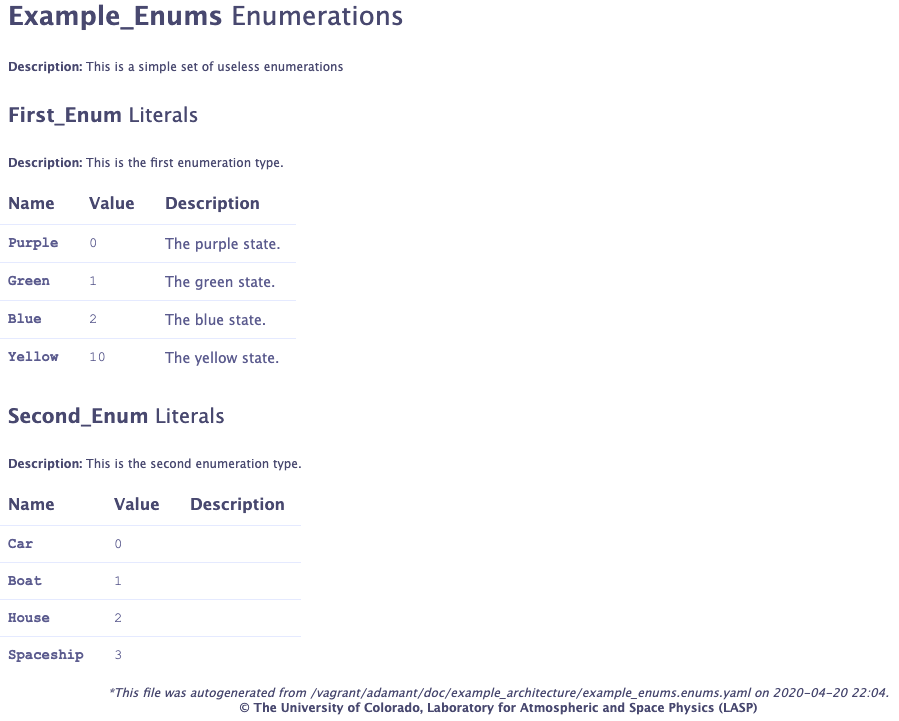
\includegraphics[width=\textwidth]{images/enumshtml.png}
\vspace{5mm} %5mm vertical space

To build the PDF documentation run:

\vspace{5mm} %5mm vertical space
\begin{minted}{text}
> redo build/pdf/example_enums.pdf
\end{minted}
\vspace{5mm} %5mm vertical space

Which produces a PDF output that looks like the following. \\

\noindent\makebox[\linewidth]{\rule{\textwidth}{0.4pt}}
\input{../example_architecture/build/tex/example_enums.tex}
\noindent\makebox[\linewidth]{\rule{\textwidth}{0.4pt}}

\subsubsection{Using Enumerations In Packed Types}

An Adamant-modeled enumeration can be used in a packed record or packed array just like a standard Ada-defined enumeration. Below is an example. We modified the \textit{example\_record} to contain two new fields, one that holds the enumeration, and another that holds some padding bits to make sure the packed record is byte aligned. The new file is called \textit{enum\_record.record.yaml} and is shown here:

\yamlcodef{../example_architecture/enum_record.record.yaml}

Note how the format used for the Adamant-modeled enumeration is \texttt{E4}. The \texttt{E} must be used when the type is an enumeration, or a modeling error will be thrown.

\subsubsection{Enumeration Python Class}

For each enumeration in an enumeration model, Adamant provides a python enumeration class. For space-based applications, these python classes are meant as ``ground" tools, or tools which assist with some task related to the deployed embedded system such as testing, parsing data, sending commands, etc. See Section \ref{Ground Tools} for more details. To build the python class for an enumeration model run:

\vspace{5mm} %5mm vertical space
\begin{minted}{text}
> redo build/py/example_enum.py
\end{minted}
\vspace{5mm} %5mm vertical space

The resulting autocode is shown below:

\pythoncodef{../example_architecture/build/py/example_enums.py}

The resulting enumeration classes inherit from the Adamant base class \texttt{EnumBase}, which in turn inherits from the python \texttt{enum.Enum} class. The python class contains the numeric definitions for each of the enumeration literals. It also includes the following helpful methods:

\vspace{5mm} %5mm vertical space
\begin{spaceditemize}
  \item \textbf{\texttt{to\_string}} - Equivalent to the Ada \texttt{Representation.Image} function; creates a human readable version of the enumeration.
  \item \textbf{\texttt{to\_tuple\_string}} - Equivalent to the Ada \texttt{Representation.To\_Tuple\_String} function; creates a log-friendly string of the enumeration.
\end{spaceditemize}
\vspace{5mm} %5mm vertical space

An example of how these classes can be used is shown below in a file called \textit{test.py}:

\pythoncodef{../example_architecture/enum_py/test.py}

The test code tests that initializing an enumeration class with a value outside of the enumeration range fails with a python \texttt{ValueError} exception. \\

Note the call at the top of the script to \texttt{pydep.build\_py\_deps()}. This Adamant python module does two useful things: 1) it searches the python program for any autocoded dependencies and uses \texttt{redo} to build them and 2) adds any autocoded dependencies automatically to the \texttt{PYTHONPATH} so they can be imported without error. It is important to run this function as the first line of any Adamant python script that will use autocoded python classes. \\

The script can be run with the command:

\vspace{5mm} %5mm vertical space
\begin{minted}{text}
> python test.py
\end{minted}
\vspace{5mm} %5mm vertical space

and produces the following output:

\vspace{5mm} %5mm vertical space
\inputminted{text}{../example_architecture/enum_py/output.txt}
\vspace{5mm} %5mm vertical space

Python classes can also be autogenerated for packed records and packed arrays, see Section \ref{Packed Record Python Class}.

\subsubsection{Enumeration MATLAB Class}

For each enumeration in an enumeration model, Adamant provides a MATLAB enumeration class. For space-based applications, these MATLAB classes are meant as ``ground" tools, or tools which assist with some task related to the deployed embedded system such as testing, parsing data, sending commands, etc. See Section \ref{Ground Tools} for more details. To build the MATLAB class for an enumeration model run:

\vspace{5mm} %5mm vertical space
\begin{minted}{text}
> redo build/m/Example_Enums
\end{minted}
\vspace{5mm} %5mm vertical space

This will build a .m file for each enumeration defined in \textit{example\_enums.enums.yaml}, since MATLAB requires that each enum class definition be contained within its own .m file. The resulting autocode for \textit{build/m/Example\_Enums/First\_Enum.m} and \textit{build/m/Example\_Enums/Second\_Enum.m} shown below: \\

\textit{First\_Enum.m}
\matlabcodef{../example_architecture/build/m/Example_Enums/First_Enum.m} \\

\textit{Second\_Enum.m}
\matlabcodef{../example_architecture/build/m/Example_Enums/Second_Enum.m}

The MATLAB class contain the numeric definitions for each of the enumeration literals.

An example of how these classes can be used is shown below in a file called \textit{test.m}:

\matlabcodef{../example_architecture/enum_m/test.m}

The script can be run with the command:

\vspace{5mm} %5mm vertical space
\begin{minted}{text}
>> test
create enums:
    Green
    Yellow
    Car
    Spaceship
passed.
\end{minted}
\vspace{5mm} %5mm vertical space

MATLAB classes can also be autogenerated for packed records and packed arrays, see Section \ref{Packed Record MATLAB Class}.

\subsection{Packed Registers}

Adamant packed records and arrays allow a developer to specify the exact bit representation of a type within the Ada language. This feature makes it ideal for describing hardware register definitions and memory mapped IO. However, using regular packed record types \texttt{.T} (for big endian machines) and \texttt{.T\_Le} (for little endian machines) is often not enough to ensure correct interaction with the hardware. On many hardware platforms, registers must be read in their entirety with a single CPU instruction without interruptions from other tasks in the system, and without reads and writes being removed by compiler optimizations. Adamant provides a method for circumventing these issues using special Volatile, Atomic, and Register packed records and packed record sets, which are described in the subsequent sections.

\subsubsection{Volatile, Atomic, and Volatile Full Access in Ada}

The Ada language provides a few facilities for specifying how an object or type should be read or written to memory. These come in the form of representation pragmas (or aspects) that specify the properties of the type of object. The important facilities used within Adamant are \texttt{Volatile}, \texttt{Atomic}, and \texttt{Volatile\_Full\_Access}. Descriptions of each is provided below:

\vspace{5mm} %5mm vertical space
\begin{itemize}
  \item \texttt{\textbf{Volatile}} - \texttt{Volatile} is a representation pragma that can be used with types and variables to specify that the variable in question may suddenly change in value. For example, this may occur due to a device writing to a shared buffer. When this pragma is used, the compiler must suppress any optimizations that would interfere with the correct reading of the volatile variables. For example, two successive readings of the same variable cannot be optimized to just one or reordered. 
  \item \texttt{\textbf{Atomic}} - \texttt{Atomic} is a representation pragma that can be used with types and variables to specify that the code generated must read and write the type or variable from memory atomically, i.e. as a single/non-interruptible operation. It implies \texttt{pragma Volatile}, the difference is that \texttt{pragma Atomic} is stronger: the compilation must fail if the variable cannot be updated atomically. In some cases it can be used for tasking, but for communication of Ada tasks it is safer to use protected types or other synchronization primitives. Note: It is almost ALWAYS wrong to use \texttt{Atomic} variables for tasking. If you choose to do so, proceed with caution.
  \item \texttt{\textbf{Volatile\_Full\_Access}} - This is similar in effect to \texttt{pragma Volatile}, except that any reference to the object is guaranteed to be done only with instructions that read or write ALL the bits of the object. Furthermore, if the object is of a composite type, then any reference to a subcomponent of the object is guaranteed to read and/or write ALL the bits of the object. The intention is that this be suitable for use with memory-mapped I/O devices  and register on some machines. Note that there are two important respects in which this is different from \texttt{pragma Atomic}. First a reference to a \texttt{Volatile\_Full\_Access} object is not a sequential action in the RM 9.10 sense and, therefore, does not create a synchronization point. Second, in the case of \texttt{pragma Atomic}, there is no guarantee that all the bits will be accessed if the reference is not to the whole object; the compiler is allowed (and generally will) access only part of the object in this case. In Adamant, \texttt{Volatile\_Full\_Access} is used for register type definitions.
\end{itemize}
\vspace{5mm} %5mm vertical space

In general, \texttt{Volatile\_Full\_Access} should be used for all hardware interaction, particularly if you need to guarantee that an entire register is read from/written to (instead of just a portion). \texttt{Volatile} should be used when you want to access a memory region that could be written to / read from by some external source, such as an FPGA shared buffer. \texttt{Atomic} should be used rarely, but is sometimes useful if a variable needs to be shared between interrupt handlers, where using a protected object may impose too much of a performance penalty. You should almost always prefer the use of protected objects over \texttt{Atomic} variables. \\

These pragmas can be applied to types, ie.

\vspace{5mm} %5mm vertical space
\begin{minted}{ada}
-- Volatile integer:
type V_Int is new Integer 
  with Volatile => True;
-- Array with atomic components:
type A_Array is new array(Natural range 1 .. 10) of Positive 
  with Volatile_Components => True;
\end{minted}
\vspace{5mm} %5mm vertical space

and also to objects, ie.

\vspace{5mm} %5mm vertical space
\begin{minted}{ada}
-- Integer register:
a : Integer 
  with Volatile_Full_Access => True;
for a'Address use Some_Hw_Addr;
-- Volatile integer:
b : Integer := 0 
  with Volatile => True;
\end{minted}
\vspace{5mm} %5mm vertical space

The following section will show how to use Adamant packed records and arrays with these pragmas already predefined.

\subsubsection{Packed Register Type}

In Adamant, when you create a packed record or array a volatile version of that type is always created called \texttt{.Volatile\_T} (big endian) or \texttt{.Volatile\_T\_Le} (little endian). You may have noticed these definitions in section \ref{Packed Record Ada Specification}. These can be used to specify a volatile version of the record, which when accessed in a volatile manner. \\

\texttt{Atomic} packed records, \texttt{.Atomic\_T} or \texttt{.Atomic\_T\_Le}, and \texttt{Volatile\_Full\_Access} packed records, \texttt{.Register\_T} or \texttt{.Register\_T\_Le}, are only defined when the size of the packed record is exactly 8, 16, or 32 bits in length. The reason for this is that Ada can only ensure that at type is atomic or \texttt{Volatile\_Full\_Access} if the type is of one of those sizes. Since registers used on embedded targets for Adamant are almost always 32 bits in length, a packed record register definition is always created with a \texttt{.Register\_T} and \texttt{.Register\_T\_Le} type that should be used to access any hardware defined by that type. \\

A typical 32-bit hardware register definition is provided below:

\yamlcodef{../example_architecture/example_register.record.yaml}

Since the size is 32 bits in length, the special \texttt{Atomic} and \texttt{Register} types are created with the expected Ada defined representation pragmas (aspects).

\adacodef{../example_architecture/build/src/example_register.ads}

Notice the new types \texttt{.Atomic\_T}, \texttt{.Atomic\_T\_Le}, \texttt{.Register\_T}, and \texttt{.Register\_T\_Le}. The register type can be used as follows:

\adacodef{../example_architecture/record_register/main.adb}

Notice that we have defined the register type for a little endian machine and tied it to a specific hardware address. We then access the register by reading the entire register into a copy, modifying that copy, and then writing the register back into place. Generally, this is the pattern that should be followed when working with hardware registers, as it is most efficient and readable. However, the second set of code also words due to the \texttt{Volatile\_Full\_Access} type specification. Two bits are read from the register and then a 14-bit number is written. With a normal packed record, this operation would fail since likely the compiler would not read or write the entire 32-bit register during the operation, resulting in unintended behavior within the hardware. However, with the \texttt{.Register\_T\_Le} type, the entire register is read for each of the two comparisons and a read-modify-write sequence is used to set the 14-bit threshold. While this works as intended, the first pattern is usually preferred as it will result in more efficient code.

\subsubsection{Packed Register Set}

The previous section demonstrated how to define and access a hardware register using Adamant packed records. Complex hardware devices are often defined as a set of registers. While a set of registers can be defined as a regular packed record in Adamant, you will not gain access to the \texttt{Volatile\_Full\_Access} pragma for each of the individual registers which could result in errant reads/writes of the registers. The proper way to define a register set in Adamant is to create an encompassing packed record which holds each of the individual register components. \\

The following defines a register set which consists of three registers of the type \texttt{Example\_Register.Register\_T\_Le}, except for the last which is \texttt{Example\_Register.Register\_T}. Mixed endianness is allowed, if unusual. The \texttt{Register} types are used to ensure that the compiler produces code for accessing each individual register by reading/writing all bits of the register atomically.

\yamlcodef{../example_architecture/example_register_set.record.yaml}

Note that when you define a packed record with a \texttt{Volatile}, \texttt{Atomic}, or \texttt{Register} type, ALL components of that packed record must be either \texttt{Volatile}, \texttt{Atomic}, or \texttt{Register}. It does not make sense to define a record with only a portion of the record being \texttt{Volatile}, \texttt{Atomic}, or \texttt{Register} type. \\

The resulting generated code is different from that normally produced for a packed record. Below is the output \textit{example\_register\_set.ads}:

\adacodef{../example_architecture/build/src/example_register_set.ads}

First, note that there is no \texttt{U} type provided. Since the record is only made up of packed records, there is no such thing as an unpacked definition. There is also not a \texttt{T} or \texttt{T\_Le} type available. Since all components of this record are \texttt{Volatile}, or \texttt{Atomic} or \texttt{Register} (which imply \texttt{Volatile}), the entire packed record is also considered \texttt{Volatile}. For this reason, only a \texttt{Volatile\_T} or \texttt{Volatile\_T\_Le} type are provided. Note that the difference between the big endian and little endian versions of these type is meaningless. The endianness of each individual register is defined by the type of that register as defined in the yaml. In this case, the first two registers are little endian and the last one is big endian. \\

In the case where all the item types of the register set are defined as a \texttt{Register} a special type is created for the register set called \texttt{Register\_T} and \texttt{Register\_T\_Le}. These are functionally the same type as \texttt{Volatile\_T} or \texttt{Volatile\_T\_Le}, but since these types are only generated when the entire register set consists of \texttt{Register} types, using the \texttt{Register} type is preferable, since you can use it to ensure that all internal items are of type \texttt{Register}. \\

The register set can be used like any normal packed record, except that accessing the individual records is safe for the hardware due to the underlying \texttt{Volatile\_Full\_Access} type specification. The following example expands on the example provided in the previous section for a single register. This time we access different registers found within the register set.

\adacodef{../example_architecture/record_register_set/main.adb}

\subsubsection{Packed Register Arrays}

If all the registers in a register set are of the same type you can used a packed array instead of a packed record to described the hardware. For example, to describe a set of 10 32-bit registers that should be interpreted as unsigned integers you can define the following packed array.

\yamlcodef{../example_architecture/example_register_array.array.yaml}

This model produces the following generated code:

\adacodef{../example_architecture/build/src/example_register_array.ads}

Because the array components are 32-bits in size, the autocode includes an \texttt{Atomic\_T}, \texttt{Atomic\_T\_Le}, \texttt{Register\_T}, and \texttt{Register\_T\_Le} types which can be used to provide \texttt{Atomic} type access. Note that for arrays of 32-bit components an \texttt{Atomic} component type is equivalent to \texttt{Volatile\_Full\_Access} array component type. Ada does not support specifying the latter, but Adamant provides a type for the \texttt{Atomic} type with the name \texttt{Register}. \\

You can also declare a register array that is made up of packed register record elements. For example, the following array can be defined:

\yamlcodef{../example_architecture/example_packed_register_array.array.yaml}

In this case we have an array of 10 elements, each of \texttt{Register\_T\_Le} type. The following autocode is produced:

\adacodef{../example_architecture/build/src/example_packed_register_array.ads}

This is treated similar to a packed register set, described in the previous section. Because the array is made up of packed \texttt{Register} components, an \texttt{U}, \texttt{T}, and \texttt{T\_Le} type are not provided. Instead a \texttt{Volatile\_T}, and \texttt{Volatile\_T\_Le} type is provided, since the internal array components are also \texttt{Volatile}. Because all the array components are of type \texttt{Register}, a type \texttt{Register\_T} and \texttt{Register\_T\_Le} is also provided. As before, the endianness used of the type at this level is not important. The endianness of reads and writes is determined by the array component type, in this case little endian. \\

The code below illustrates using these arrays to read/write registers.

\adacodef{../example_architecture/array_register_set/main.adb}

\newpage
\section{Components} \label{Components}

Adamant is a component-based framework. Component-based frameworks approach application design as a set of reusable functional or logical entities called components, which expose well-defined interfaces for inter-component communication. The motivation behind Adamant's component-based architecture is thoroughly discussed in the \href{https://github.com/lasp/adamant/blob/main/doc/architecture_description_document/architecture_description_document.pdf}{\textcolor{blue}{Architectural Description Document}}. An understanding of the concepts in that document is required before diving into building your own component, which is the purpose of this section. \\

The beginning of this section outlines the different component patterns that are common within Adamant constructed software. The following list is copied from the Archectural Description Document and specifies the User Guides section where each component pattern is presented.

\vspace{5mm} %5mm vertical space
\begin{itemize}
  \item \textbf{Passive without Queue}, Section \ref{Creating a Passive Component} - This type of component will only execute when a caller invokes one of its connectors. This type of component is typically used to provide a synchronous service to other components, such as getting the system time, or updating a parameter database.
  \item \textbf{Passive with Queue}, Section \ref{Creating a Queued Component} - Like the \textit{Passive without Queue} component, this component will also only execute when called. However, because it has a queue, this component is typically used to respond to asynchronous messages at a scheduled time. Execution is commonly invoked through a ``schedule" connector, which tells the component to service its queue and possibly do other periodic work. This design is ideal for components that need to be executed with cyclic real-time deadlines, such as a control loop.
  \item \textbf{Active with Queue}, Section \ref{Creating an Active Component} - The default behavior of components that follow this pattern is to block on their queue and only wake up and do work when a message is received asynchronously. This type of component is ideal for components that run at a specified priority and receive asynchronous messages, such as a logger. This default task behavior can be overridden if necessary by the developer, but this should be avoided if possible, since the component diagram will not give insight into this custom behavior.
  \item \textbf{Active without Queue}, Section \ref{Creating a Background Component} - Unlike \textit{Active with Queue} components, there is no default behavior for the \textit{Active without Queue} task. In this case, the developer must define the code which executes on the component's thread. This component pattern is uncommon, and not recommended, since the component's behavior cannot be readily ascertained from its diagram. However, this design might be useful for components that run in the background, but receive no asynchronous input, such as a memory scrubber.
\end{itemize}
\vspace{5mm} %5mm vertical space

Each pattern builds on the previous pattern. It is recommended that for best understanding of an active component with queue to first read the sections for a passive component without queue followed by a passive component with queue, before proceeding to the active component with queue section.

\subsection{Creating a Passive Component} \label{Creating a Passive Component}

In this section we will be discuss how to create a component called \textit{example\_component}. We will start simple, and then add (and subtract) features throughout subsequent sections to demonstrate the features of Adamant components and how to use them. \\

Note: These sections often use the phrase building ``components". To be more specific, what we are really creating here are \textit{component types}, which can be thought of as analogous to a classes in the object-oriented sense. Later, in Section \ref{Assemblies}, we will talk about creating instantiations of these \textit{component types} called \textit{component instances}. \textit{Component instances} are analogous to an object in the object-oriented sense. This distinction is important because more than one \textit{component instance} can be created from a single \textit{component type}. From now on, we will talk about building ``components," but remember, we are actually creating \textit{component types}. \\

Components are usually created in their own directory. Let's create one for our example component.

\vspace{5mm} %5mm vertical space
\begin{minted}{text}
> mkdir example_component  # make component directory
> cd example_component 
> touch .all_path          # add directory to build path
\end{minted}
\vspace{5mm} %5mm vertical space

To define a component in this directory, a developer must create a YAML model file in the form \textit{name.component.yaml} where \textit{name} is the desired name of the \textit{component type}. Below is the component definition for the \textit{example\_component}. This definition is stored in a file called \textit{example\_component.component.yaml} within this new directory.

\yamlcodef{../example_architecture/example_component/example_component.component.yaml}

Comments are included in the model to explain whether or not each field is optional or required. A component must always specify its \textit{execution}. The details on component \textit{execution} are discussed in the \href{https://github.com/lasp/adamant/blob/main/doc/architecture_description_document/architecture_description_document.pdf}{\textcolor{blue}{Architectural Description Document}} and copied below for reference:

\vspace{5mm} %5mm vertical space
\begin{itemize}
  \item \textbf{Passive} - \texttt{Passive} components do not have a thread of their own and are expected to execute on the thread of their connector invokers.
  \item \textbf{Active} - \texttt{Active} components contain their own thread on which they execute.
  \item \textbf{Either} - \texttt{Either} components are designed to function either as \texttt{passive} or \texttt{active} components. Which \textit{execution} type a component will get resolved to is decided at the assembly level.
\end{itemize}
\vspace{5mm} %5mm vertical space

The component we have defined above is a \textit{passive} component, which means that it does not have its own thread of execution, and will only execute on the thread of any connector \textit{invokers}. In this case, the only way the component can execute is through a call to its \texttt{Tick\_T\_Recv\_Sync} connector. \\

The most important part of any component model is its connector definition. This YAML model declares \textit{example\_component} with three connectors. One connector is an \textit{invokee} connector of type \texttt{Tick.T}. This connector is a scheduling connector. When the connector is called the component does its ``work". The component also has two \textit{invoker} connectors. The first is used to fetch the system time via type \texttt{Sys\_Time.T}. The second is used to send out a packet of type \texttt{Packet.T}. \\

In the model, for each connector we have not only defined the connector \textit{types} (and \textit{return\_types}), which are all \textit{packed records} (see Section \ref{Packed Records}), but we also define the connector \textit{kind}. Connector \textit{kinds} are discussed thoroughly in the \href{https://github.com/lasp/adamant/blob/main/doc/architecture_description_document/architecture_description_document.pdf}{\textcolor{blue}{Architectural Description Document}} but a diagram of all possible connector kinds is shown below for reference:

\vspace{5mm} %5mm vertical space
\begin{figure}[H]
  \includegraphics[width=1.0\textwidth,center]{../example_architecture/build/eps/connector_kinds.eps}
  \caption{Example component diagram to demonstrate different connector \textit{kinds}}
\end{figure}
\vspace{5mm} %5mm vertical space

Recall that connector \textit{kinds} are used to specify the direction and synchroneity of data flow along a connector. Connector \textit{kinds} fall into one of four categories, whose names correspond to the direction of the data flow with respect to the \textit{invokee}. A summary of the available connector \textit{kind} pairs are shown below.

\vspace{5mm} %5mm vertical space
\begin{center}
  \begin{tabular}{ | l | c | c | c | c |}
    \hline
    \textbf{Category} & \textbf{Invoker Kind} & \textbf{Invokee Kind} & \textbf{Has \textit{type}?} & \textbf{Has \textit{return\_type}?} \\ \hline
    In & \texttt{send} & \texttt{recv\_sync} or \texttt{recv\_async} & yes & no \\ \hline
    Out & \texttt{get} & \texttt{return} & no & yes \\ \hline
    In Return & \texttt{request} & \texttt{service} & yes & yes \\ \hline
    In Out & \texttt{provide} & \texttt{modify} & yes & no \\ \hline
  \end{tabular}
\end{center}
\vspace{5mm} %5mm vertical space

The chosen connector \textit{kind} pair determines whether or not a \textit{type}, \textit{return\_type}, or both is required for the connector definition. Note that a model error will be produced if you fail to comply with the table above, so have no fear of making mistakes. \\

The definition of the \texttt{Packet\_T\_Send} connector specifies the optional field \textit{count}. The \textit{count} field is used to specify an \textit{arrayed} connector. When not specified, the connector \textit{count} is assumed to be 1, which means that the connector is not arrayed. If a positive value greater than 1 is provided, then the component is created with an array of connectors of the specified size. If the \textit{count} is defined as 0, as is the case here, than the connector array size is said to be \textit{unconstrained} and will be set during the component's instantiation within an assembly, see Section \ref{Assemblies}. In this case we have created an unconstrained array of \texttt{Packed.T} \textit{send} connectors, which can be called by index. \\

Note that we have defined an optional \textit{name} for the \texttt{Tick\_T\_Recv\_Sync} connector. If no \textit{name} is specified then Adamant will generate a name for the connector in the form \textit{type\_kind} where \textit{type} is the connector type with any ``."s replaced by ``\_"s and \textit{kind} is the connector's \textit{kind}. In general, it is considered good practice to NOT provide names for connectors, as the autocoded names are informative and follow a convention that provides information about of the connector's form and function. However, there are certainly exceptions to this rule. Sometimes defining a custom name makes more sense, like in the case where a component has two connectors of the same \textit{type} that perform distinct behaviors. \\

\subsubsection{Creating a Component Diagram} \label{Creating a Component Diagram}

Components in Adamant are often presented using diagrams, which contain a visual representation of the semantics encoded in the component YAML file. A component diagram can be generated from the \textit{example\_component} model by running the following from the component directory:

\vspace{5mm} %5mm vertical space
\begin{minted}{text}
> redo build/svg/example_component.svg
\end{minted}
\vspace{5mm} %5mm vertical space

which produces an SVG diagram of the component that can be viewed in any web browser. An \textit{eps} version, which is easy to import into PDF documentation can also be constructed:

\vspace{5mm} %5mm vertical space
\begin{minted}{text}
> redo build/eps/example_science.eps
\end{minted}
\vspace{5mm} %5mm vertical space

and the output is shown below:

\vspace{5mm} %5mm vertical space
\includegraphics[width=1.0\textwidth,center]{../example_architecture/example_component/build/eps/example_component.eps}
\vspace{5mm} %5mm vertical space

As can be seen, the \textit{example\_component} is \textit{passive} because the outline around the component is not bold. It has a single \textit{invokee} connector named \texttt{Tick\_T\_Recv\_Sync} and two \textit{invoker} connectors called \texttt{Sys\_Time\_T\_Get} and \texttt{Packet\_T\_Send}. \texttt{Packet\_T\_Send} is denoted as an arrayed connector using the \texttt{[<>]} notation, where \texttt{<>} signifies that the connector array size is unconstrained, and will be determined by the assembly.

\subsubsection{Anatomy of a Component} \label{Anatomy of a Component}

Before we begin to implement the \textit{example\_component}, we need to understand how a component is constructed using the Ada language. Below is a UML-like class diagram that shows the Ada packages that make up a component.

\vspace{5mm} %5mm vertical space
\begin{figure}[H]
  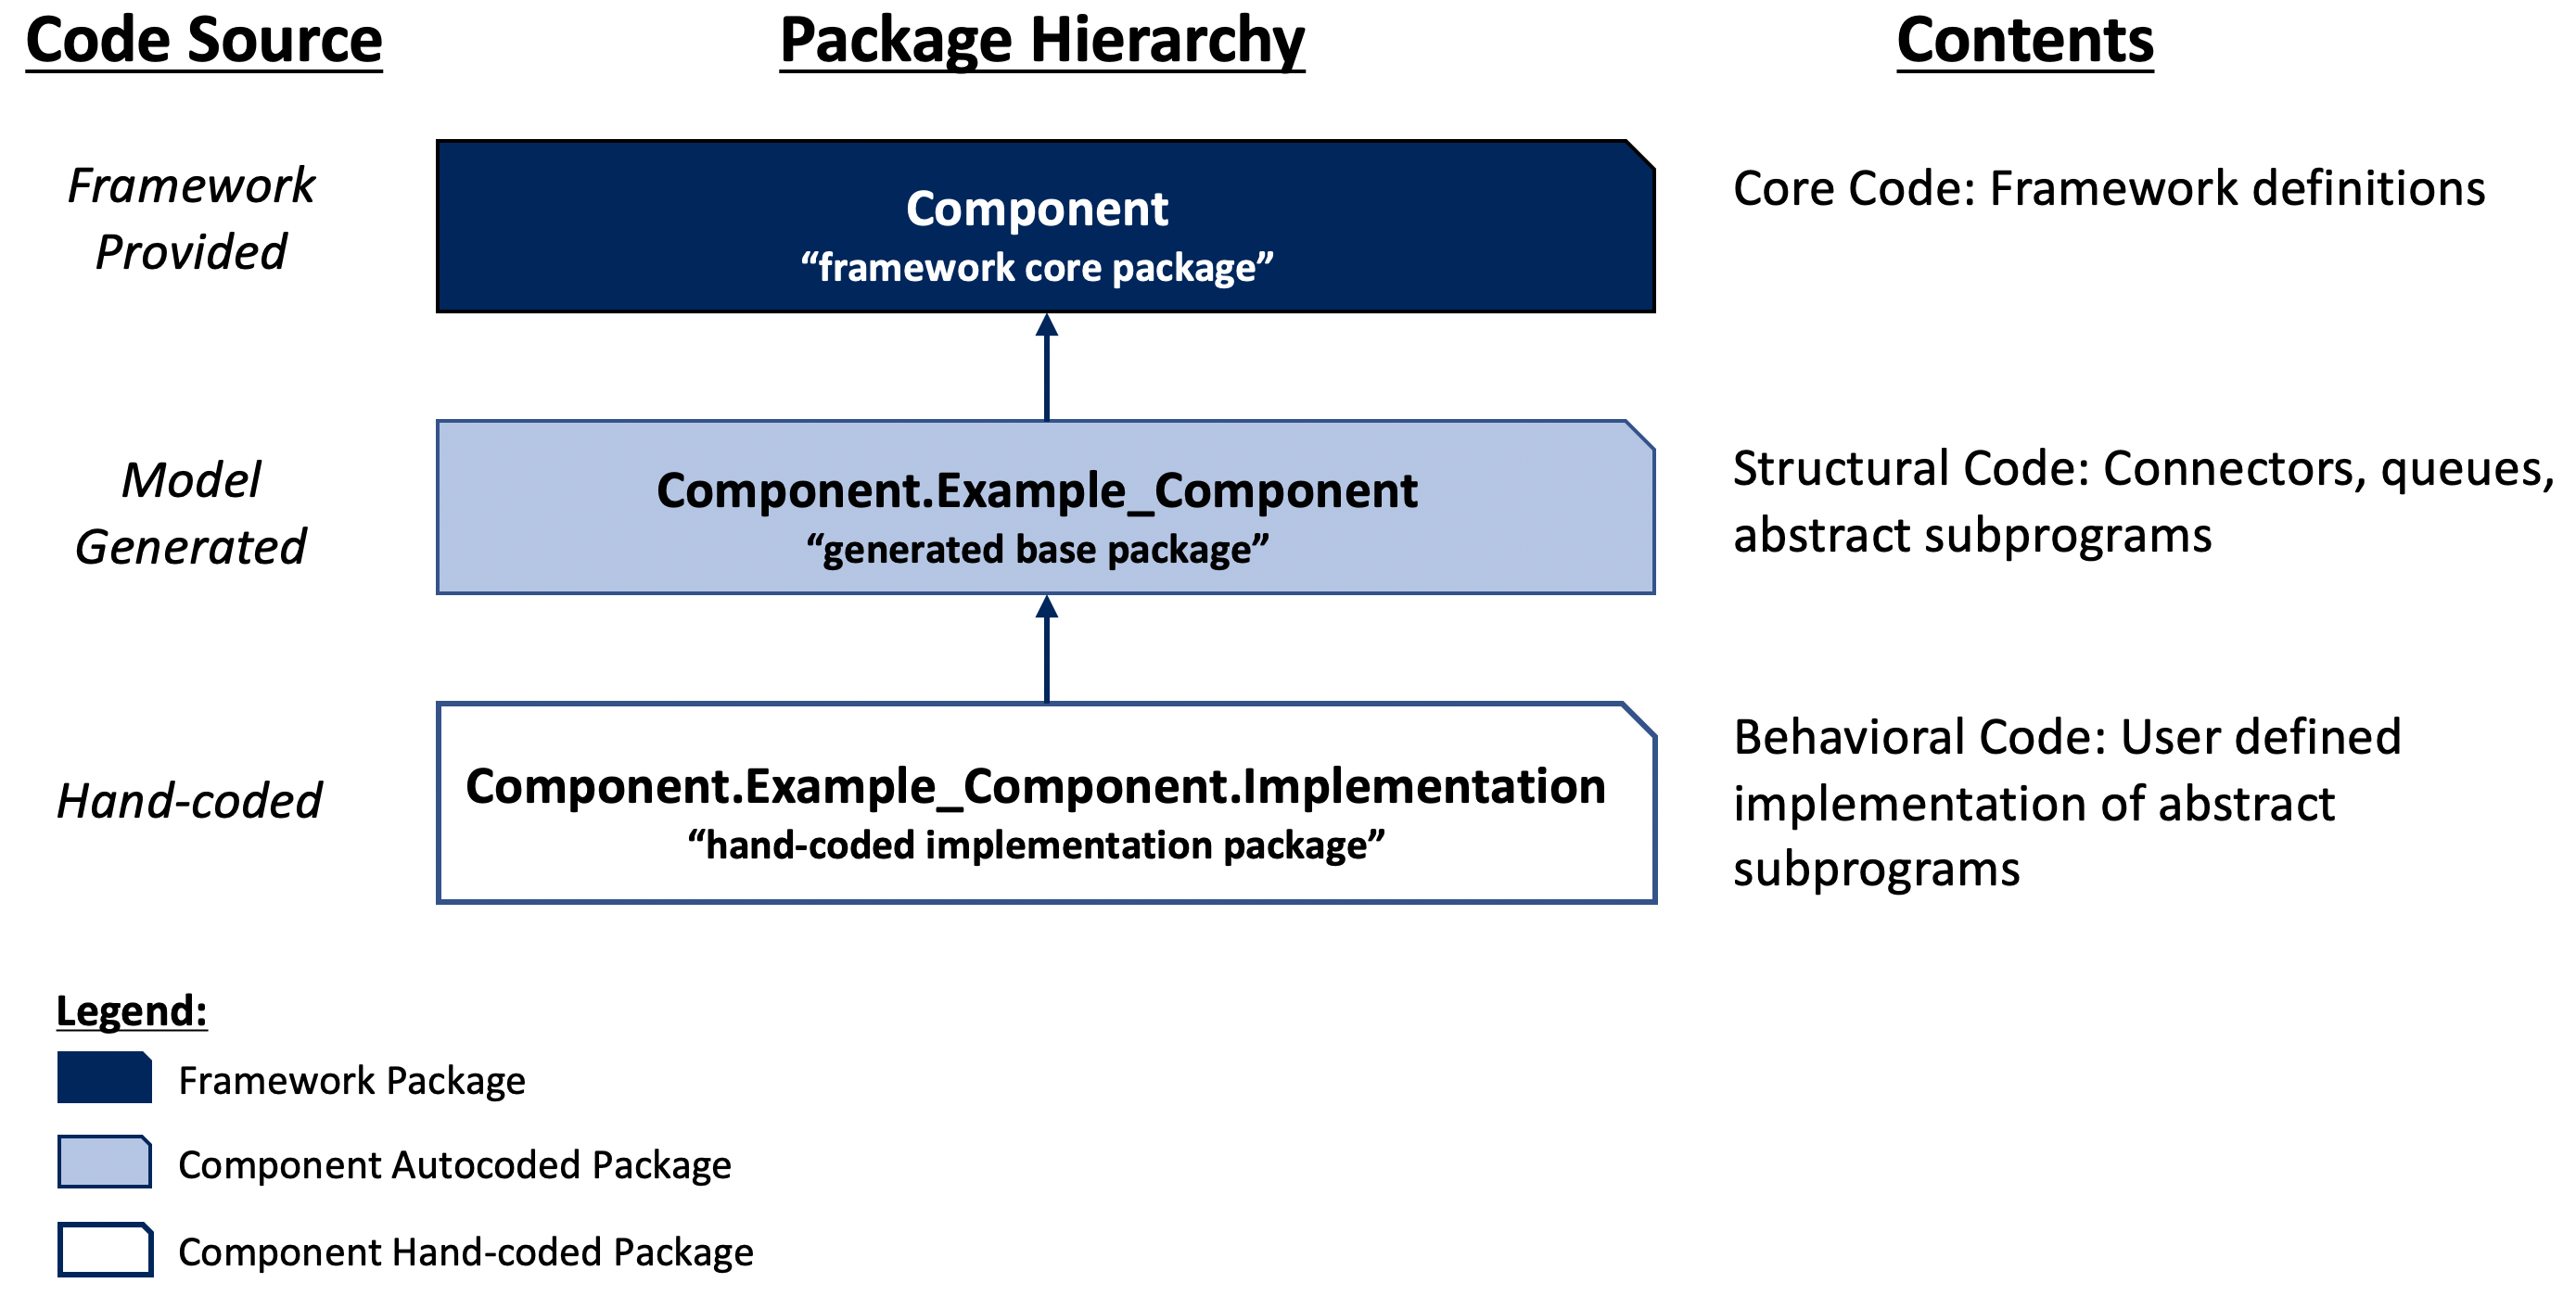
\includegraphics[width=1.00\textwidth,center]{images/componentpackages.png}
  \caption{This diagram shows the three different Ada packages that make up a component.}\label{Component Package Diagram}
\end{figure}
\vspace{5mm} %5mm vertical space

The top package in the diagram is also the upper most ``parent" in an object-oriented sense. Each subsequent package is a child package of the first, which in Ada means they have access to the private definitions within the parent package. In addition, each subsequent package includes a derived tagged type called \texttt{Instance}, that derives from the parent package \texttt{Instance}. In this way, each \texttt{Instance} type ``extends" the functionality of the parent \texttt{Instance} type. There are three inheritance levels that make up a component in Adamant, and they each serve a unique purpose. \\

The top level parent is the \texttt{Component} package, whose source can be found in the Adamant core in \textit{src/core/component}. This package includes definitions and subprograms that are shared by all components in Adamant. Most importantly, this package defines the \textit{class-wide} component type that all components inherit from. This class-wide type is what allows dynamic dispatching within components, and is the key language feature needed to implement connectors. \\

The next level is unique to every \textit{component type} definition. That is, every component YAML model generates a different version of this base package. For the YAML that we created for the \textit{example\_component} in the previous sections, an autocoded base package with the name \texttt{Component.Example\_Component} will be generated in the files \textit{component-example\_component.ads} and \textit{component-example\_component.adb}. The steps for generating these files are presented in the following section. The purpose of this package is to codify the structure defined in the model. Specifically, connectors, internal queues, and other entities defined in the model are included in the \texttt{Instance} type at this level. Furthermore, this package will contain an abstract subprogram for every \textit{invokee} connector that a component defines. These are unimplemented subprograms that MUST be implemented by an inheriting package or a compilation error will result. This feature ensures that any connectors defined in the model are actually implemented in the code, otherwise the code will not compile. \\

The final level in the package hierarchy is the hand-coded implementation package \texttt{Component.Example\_Component.Implementation}. This package includes a type \texttt{Instance} that inherits from the \texttt{Instance} type defined in the generated base package. At this level ``templates" can be autocoded to assist the developer in beginning to implement the component. Directions for generating implementation package templates can be found in Section \ref{Component Implementation Package}. In this package, the programmer is responsible for hand-coding the behavioral logic of the component. Specifically, this means implementing the abstract \textit{invokee} subprograms defined in the base package, encoding the actions that the component should take whenever these connectors are invoked from the outside. \\

The hierarchy is constructed in this way for a few primary reasons. First, it allows the vast majority of boilerplate code that you would typically find in a framework to live within the autogenerated base packages. This avoids the common copy and paste errors that boilerplate code commonly introduces, and also keeps the implementation code readable. Secondly, the use of abstract subprograms in the generated base package ensures that the implementation code is always consistent with the model that describes it. This ensures that all other products generated from the model, documentation, ground system interfaces, etc. are also consistent with the form and structure of the component. After modeling, the task left to the programmer becomes simple: hand-code the behavioral logic that gets executed when a component's connectors are called. \\

The following sections walk through the steps needed to generate the component base package, generate the implementation package templates, and compile a component to make sure it is syntactically correct.

\subsubsection{Component Base Package} \label{Component Base Package}

In this section we take a look at the component base package. Usually you will not have to build this package manually. Since this package is a dependency of the hand-coded implementation package, it will get compiled automatically when you build your hand-code. However, it is a good idea to at least take a look at the base package once, to understand what kind of things it contains. We explore it in this section, and explain some of the details. \\

To generate the base package we can run \texttt{redo} to compile it which will generate the autocode and then build it:

\vspace{5mm} %5mm vertical space
\begin{minted}{text}
> redo build/obj/Linux/component-example_component.o
\end{minted}
\vspace{5mm} %5mm vertical space

This should generate and compile two files \textit{build/src/component-example\_component.ads} and \textit{build/src/component-example\_component.adb}. Let's take a look the specification. \\

\textit{component-example\_component.ads}:
\adacodef{../example_architecture/example_component/build/src/component-example_component.ads}

The first thing to recognize is the type \texttt{Instance} which extends the type \texttt{Component.Instance}, declared in the framework's core \texttt{Component} package. The details of the \texttt{Instance} type are private, and thus listed in the private section. Also, note that the type is declared as \texttt{abstract} since it contains some abstract subprograms, ie. primitives that are unimplemented. This means that \texttt{Instance} cannot be instantiated or used by itself, since it is not a complete type. We must inherit from this type and implement the abstract subprograms before we can instantiate an object that uses this code. We will see how that is done in the next section. \\

In the public section there is also a very important abstract procedure \texttt{Tick\_T\_Recv\_Sync} which is the handler for our \texttt{Tick\_T\_Recv\_Sync} invokee connector. Note that it has the exact same name as the connector itself, so is easy to remember. This procedure MUST be implemented in the hand-coded implementation package, otherwise a compilation error will result. We will hand-code the behavior of this invokee connector handler in the following section. \\

If we look in the private section we can see that the type \texttt{Instance} is implemented as a record that contains two items. Both items are connector objects for the component's invoker connectors. A component will always contain connector objects for its invoker connectors in its base package. To make a call to these connectors there are two private, inlined procedures that are autocoded, \texttt{Packet\_T\_Send} and \texttt{Sys\_Time\_T\_Get}. These subprograms are important because they are meant to be called from the implementation package in order to call those connectors. The names of the procedures exactly match the connector names defined in the model, so they should be easy to remember when implementing your component. \\

Note that the declaration of \texttt{Packet\_T\_Send} also includes an \texttt{index} argument that is used to specify which connector in the connector array to call. Argument \texttt{index} is of type \texttt{Packet\_T\_Send\_Index} which you can see is defined as a subtype of \texttt{Positive} and thus will have a valid range from 1 to the size of the connector array. The actual size of the connector array is defined during runtime using the \texttt{Init\_Base} procedure. For more details on component base package initialization see Section \ref{Component Base Initialization}. \\

For each invoker connector there are also a few more autocoded methods that may be useful. Let's use the connector \texttt{Packet\_T\_Send} connector as an example, and explain all the autocoded subprograms related to it:

\vspace{5mm} %5mm vertical space
\begin{spaceditemize}
  \item \textbf{\texttt{Packet\_T\_Send}} - Used to call the invoker connector. If the invoker connector is not connected to another component, then this call will result in a runtime assertion.
  \item \textbf{\texttt{Is\_Packet\_T\_Send\_Connected}} - Used to check if the connector is connected to another component's connector during runtime.
  \item \textbf{\texttt{Packet\_T\_Send\_If\_Connected}} - Used to call the invoker connector, only if it is connected.
\end{spaceditemize}
\vspace{5mm} %5mm vertical space

These are the most important subprograms to keep in mind while hand-coding the implementation class, since they are used to call the invoker connectors. In general it is best to use the \texttt{Packet\_T\_Send\_If\_Connected} procedure when the connection is viewed as \textit{optional} in the assembly. If the component must absolutely be connected on that connector to function correctly, then use the standard \texttt{Packet\_T\_Send} procedure. \\

Note that \texttt{Packet\_T\_Send} and \texttt{Packet\_T\_Send\_If\_Connected} call a \textit{send}-kinded connector, and thus provide a special option \texttt{Full\_Queue\_Behavior}. This option allows the call to specify the behavior when the connector is connected to an \textit{recv\_async} connector of another component and the component's queue is full. The options are \texttt{Drop} (the default if unspecified), in which case the data is dropped, or \texttt{Wait}, in which case the call blocks and waits for the queue to no longer be full before proceeding. You should always use the option \texttt{Drop} unless you have a very good reason for using \texttt{Wait}. This keeps the execution of your code deterministic and predictable and forces the proper sizing of queues. \\

The remaining package definitions, not described in detail in the paragraphs above, can for the most part be ignored unless you are interested in understanding the inner workings. The purpose of these definitions is supply the structure necessary to make connectors work within the architecture. You can also see the implementation of these subprograms in the body \textit{build/src/component-example\_component.adb}, which is not shown here for brevity.

\subsubsection{Component Implementation Package} \label{Component Implementation Package}

Since we dived into the details of the base package in the previous section, we are now ready to write our own hand-code which extends it. After creating your component model, the steps below are often the next commands an Adamant developer runs. These commands autogenerate the implementation package templates from the component model and then copy them into the same directory as the component model.

\vspace{5mm} %5mm vertical space
\begin{minted}{text}
> redo build/template/component-example_component-implementation.ads 
> redo build/template/component-example_component-implementation.adb 
> cp build/template/* .   # copy templates into component dir
\end{minted}
\vspace{5mm} %5mm vertical space

You can also use the special \texttt{redo templates} command to do the same thing:

\vspace{5mm} %5mm vertical space
\begin{minted}{text}
> redo templates
> cp build/template/* .  # copy the template files into component dir 
\end{minted}
\vspace{5mm} %5mm vertical space

As a general convention, you should always store your hand-coded implementation package in the same directory as the component model. Never work on the files directly in \textit{build/template} since that directory will get removed when running \texttt{redo clean}. OK, let's take a look at our shiny new templates - specification file first. \\

\textit{component-example\_component-implementation.ads}:
\adacodef{../example_architecture/example_component/build/template/component-example_component-implementation.ads}

The first thing to notice here is the type \texttt{Instance} which inherits from the base package type \texttt{Example\_Component.Instance} that was presented in the previous section. If we look at the implementation of the type in the private section we can see that it is an empty record with the comment \texttt{TODO}. This is where we can add any necessary component state information including other objects, variables, etc. \\

Next, in the private section, there are a few subprograms of importance. First the \texttt{Set\_Up} function will not be discussed here; see Section \ref{Component Set Up} for details. \\

Following, there is the procedure called \texttt{Tick\_T\_Recv\_Sync}. This procedure overrides the abstract \texttt{Tick\_T\_Recv\_Sync} procedure declared in the base package in the previous section. This procedure acts as the handler function that gets called whenever the \texttt{Tick\_T\_Recv\_Sync} connector is called from an outside component. We will need to defined the behavior for this procedure in the package body. \\

Lastly, there is a \texttt{Packet\_T\_Send\_Dropped} procedure whose implementation is set to \texttt{null}, which means that when the procedure is called it does nothing. This procedure is automatically called whenever a call to \texttt{Packet\_T\_Send} gets dropped, due to a full queue, by a receiving component. By default, this procedure is implemented as \texttt{null} and the sending component performs no action. The standard Adamant convention is that the receiving component MUST implement the correct behavior to perform when something is dropped off a queue. The sender does not share that responsibility. However, this method can be implemented should the programmer deem it necessary. There are more details on dropped asynchronous connector calls in Section \ref{Creating a Queued Component}. \\

Now we are ready to take a look at the generated template for the package body. \\

\textit{component-example\_component-implementation.adb}:
\adacodef{../example_architecture/example_component/build/template/component-example_component-implementation.adb}

Simple, right?! The \texttt{Tick\_T\_Recv\_Sync} procedure gets called whenever the \texttt{Tick\_T\_Recv\_Sync} connector is invoked by an outside component. All we have to do now is hand-code what we want the component to do when this happens. \\

Note that the component implementation templates should always successfully compile. You can compile the implementation object by running:

\vspace{5mm} %5mm vertical space
\begin{minted}{text}
> redo build/obj/Linux/component-example_component-implementation.o
\end{minted}
\vspace{5mm} %5mm vertical space

or you can run \texttt{redo all} to compile every object that can be compiled for a component, including the implementation. \\

Now it is time to hand-code some behavior into the component. When the \texttt{Tick\_T\_Recv\_Sync} connector gets called we want the component to send out a packet to every component connected to it. The packet will be properly timestamped, and will contain a single byte of data that increments ever time \texttt{Tick\_T\_Recv\_Sync} is called. The first step is to add this counter to our component record, so we can keep track of its value during program execution. Our newly implemented specification looks like: \\

\textit{component-example\_component-implementation.ads}:
\adacodef{../example_architecture/example_component/component-example_component-implementation.ads}

The only modification that we made was to add the variable \texttt{counter} to the component \texttt{Instance} record. We initialize the variable to zero. Now let's take a look at the body: \\

\textit{component-example\_component-implementation.adb}:
\adacodef{../example_architecture/example_component/component-example_component-implementation.adb}

We have added the behavioral logic that gets called when the \texttt{Tick\_T\_Recv\_Sync} connector is invoked. First we declare a variable \texttt{pkt} of type \texttt{Packet.T}. You can find the definition for the \texttt{Packet.T} packed record in \textit{src/types/packet/}. We define all parts of the packet including the \texttt{Header} and the \texttt{Buffer}. Note that we set the timestamp of the packet by directly calling our invoker connector to fetch time \texttt{Self.Sys\_Time\_T\_Get}. Recall that this subprogram is implemented in the base package that was discussed in the previous section. The \texttt{Id} and \texttt{Sequence\_Count} are set to zero, and the \texttt{Buffer\_Length} is set to 1, because we are creating a packet where only the first byte of the \texttt{Buffer} is used. Finally, we initialize the entire \texttt{Buffer} byte array to zeros. \\

In the procedure body, the first step is to set the first byte of the packet data buffer, \texttt{Buffer}, to our current counter value, \texttt{Self.Counter}. Next, we iterate through every connector in the \texttt{Self.Connector\_Packet\_T\_Send} array that was declared in the base package, and then call each \texttt{Packet\_T\_Send} connector in turn, sending them each a version of the packet we created. If any of these connectors is not connected to an external component, then nothing will happen, since we used the subprogram \texttt{Packet\_T\_Send\_If\_Connected} to call the \texttt{Packet\_T\_Send} connector. Finally, we increment our counter, \texttt{Self.Counter}, so that it is one greater the next time we create a packet. \\

In the following section we will unit test this component to make sure that the logic was implemented properly.

\subsection{Unit Testing a Passive Component} \label{Component Unit Testing}

Unit testing a component is similar to unit testing a package, see Section \ref{Testing a Package}. Reading that section first will make understanding section much easier. \\

Unit testing a component is different than unit testing a package in that we want to be able to accurately simulate the execution context of a component during deployment. More specifically, we want to be able to simulate all the components that could be connected to this component in a final assembly. However, to keep things simple, Adamant achieves this simulation through a single ``reciprocal" tester component, which is attached to the component during unit test. The tester component is unique in that it contains the exact opposite connectors as the component, providing a corresponding connector for each of the component's connectors. In this way, the tester can attach to the component and holistically simulate the component's environment. Below is a diagram that demonstrates how a tester component connects to the \textit{example\_component} during unit testing.

\begin{figure}[H]
  \includegraphics[width=1.0\textwidth,center]{../example_architecture/example_component/tester/build/eps/example_to_tester_simple_view.eps}
  \caption{A diagram showing how the \textit{example\_component} is connected to its ``reciprocal" tester component during unit testing.}
\end{figure}

As can be seen, there are connections for receiving \texttt{Tick.T} and \texttt{Sys\_Time.T} and an array of 3 \texttt{Packet.T} connections from the component to the tester. The tester component itself is completely autocoded by Adamant using the component's YAML model file. The steps for creating the tester are described in following sections. \\

\subsubsection{Anatomy of a Component Unit Test} \label{Anatomy of a Component Unit Test}

Before getting into the actual mechanics of unit testing, it is important to understand all of the various Ada packages involved during unit testing. The vast majority of these packages are autogenerated by Adamant, however it is important to understand their function in order to use them properly. The diagram below is the same as Figure \ref{Component Package Diagram}, except we have added the additional packages necessary for unit testing.

\vspace{5mm} %5mm vertical space
\begin{figure}[H]
  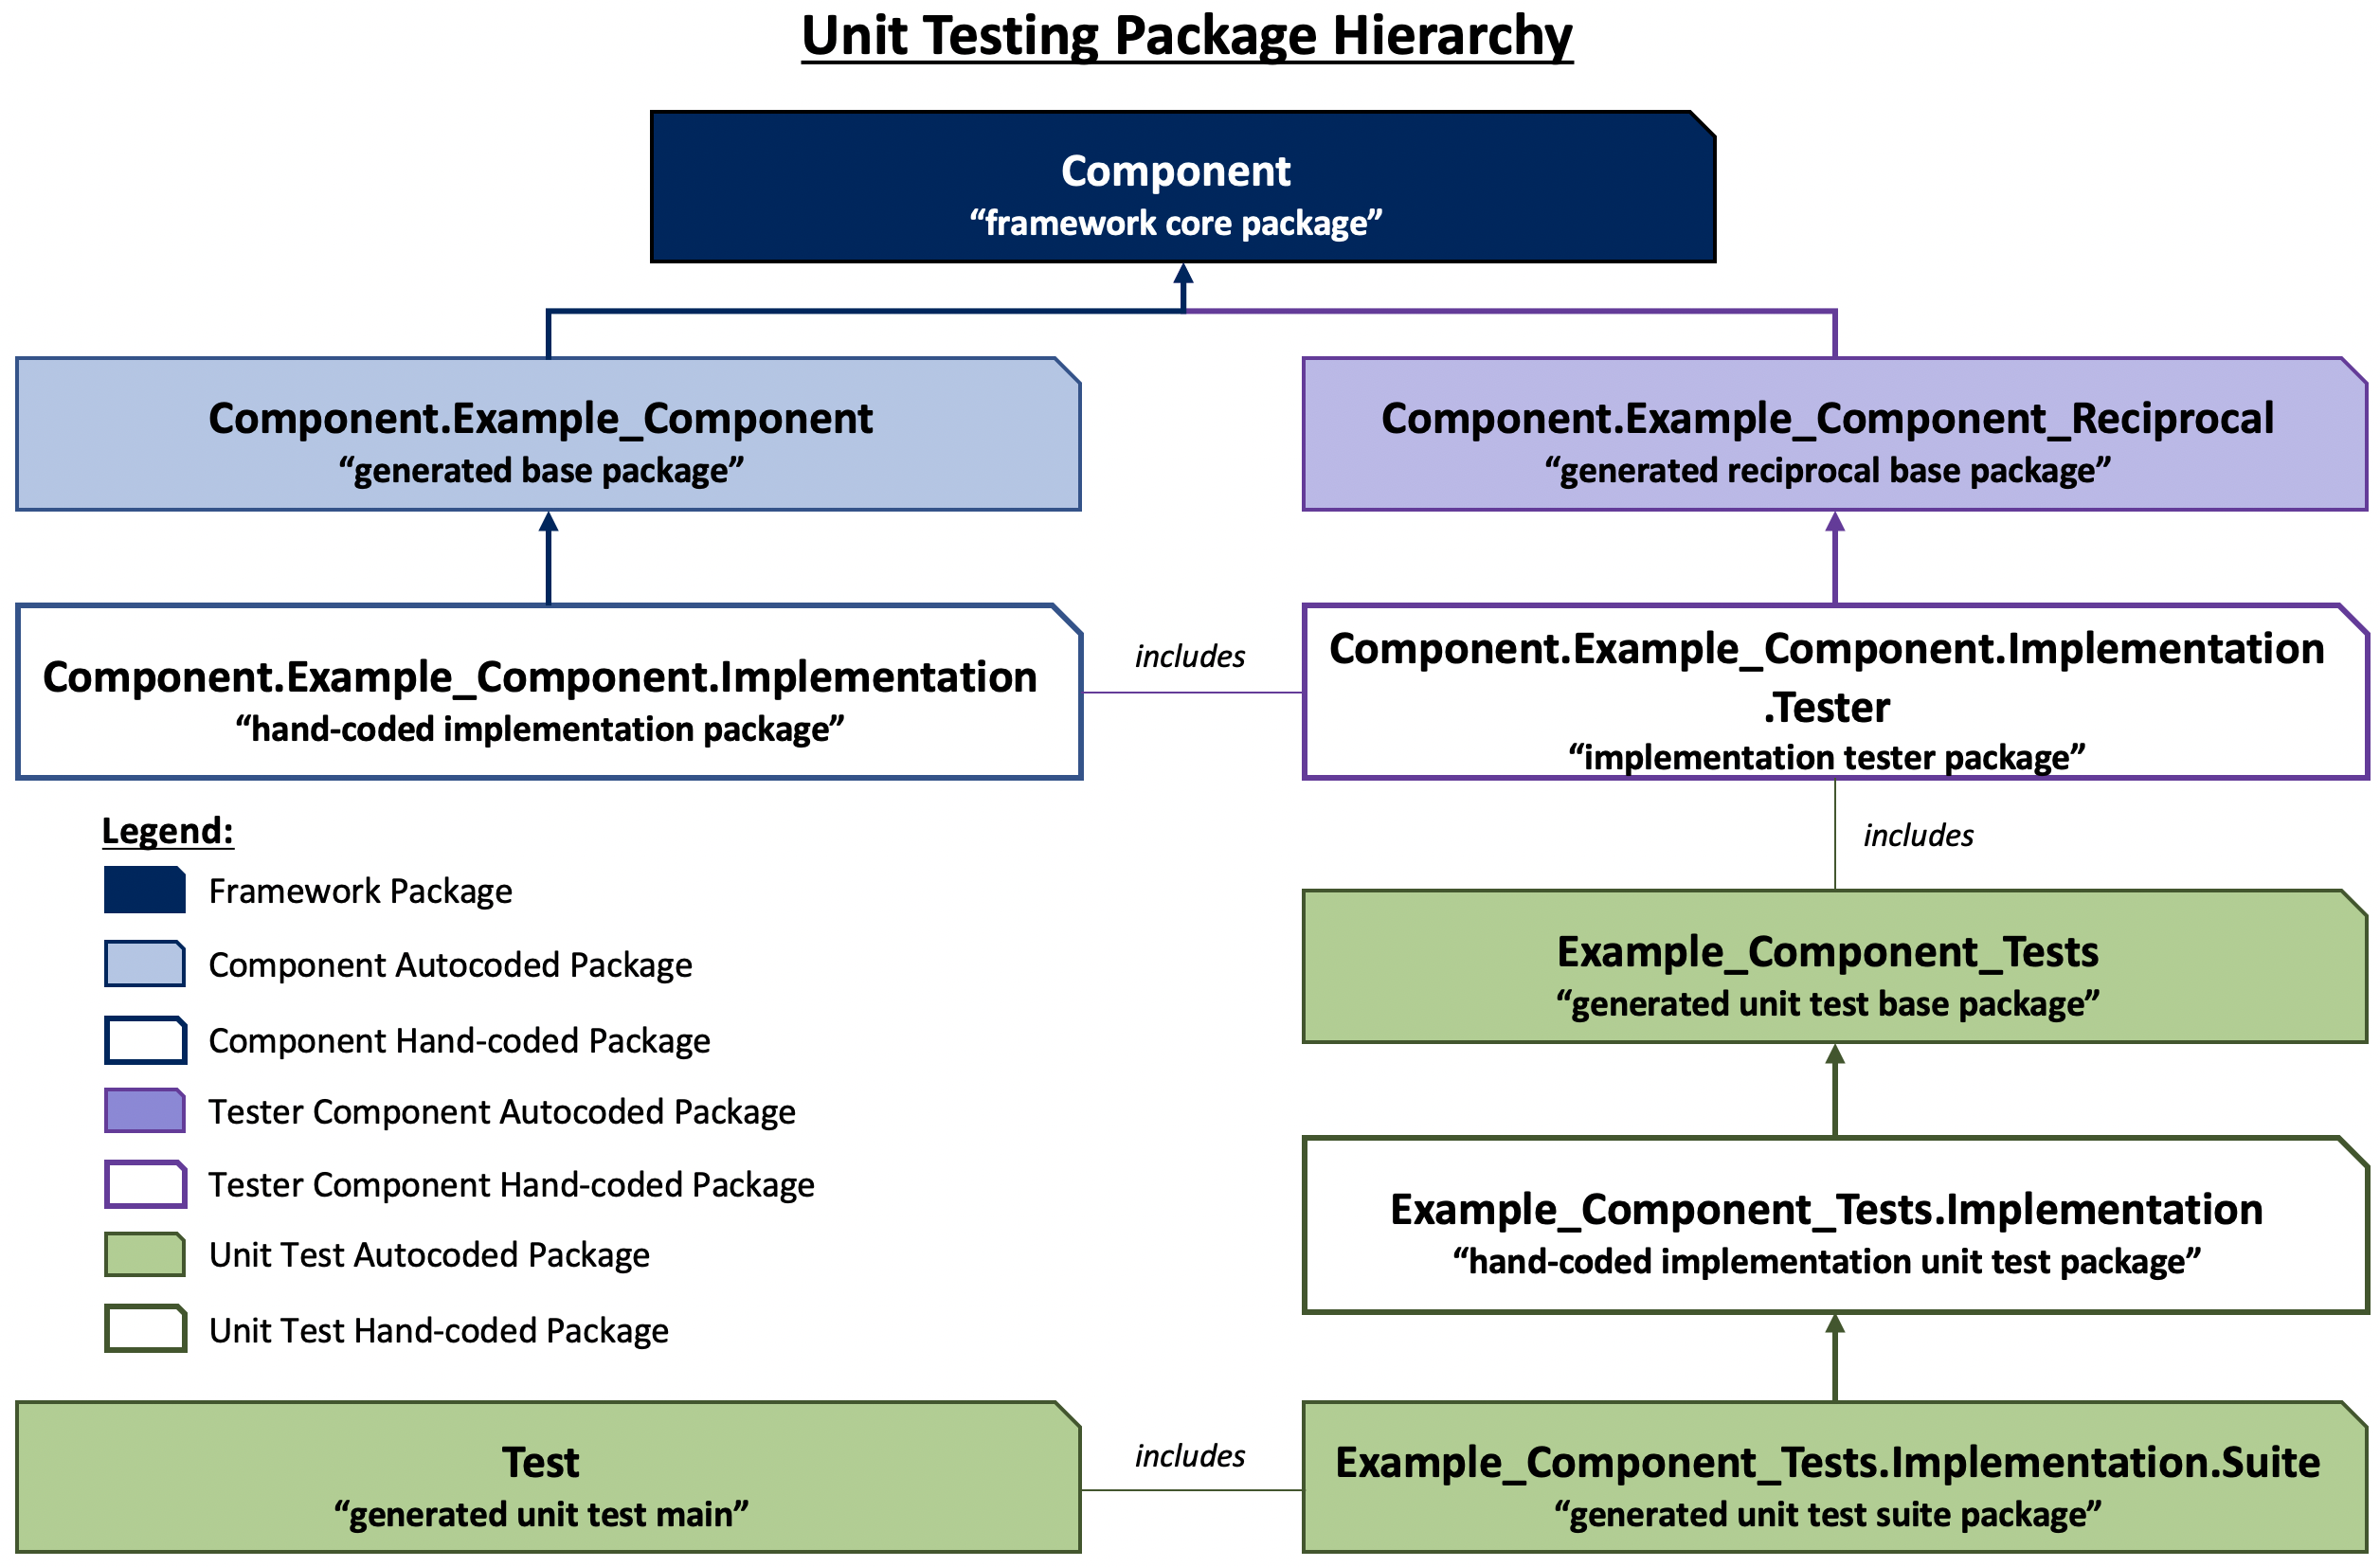
\includegraphics[width=1.00\textwidth,center]{images/testerpackages.png}
  \caption{This diagram shows the different Ada packages used to unit test a component.}
\end{figure}
\vspace{5mm} %5mm vertical space

It is important to note that two YAML models are used to generate the packages shown above, the component model, \textit{example\_component.component.yaml}, and a unit test model, \textit{example\_component.tests.yaml}. Creating the unit test model is shown in the next section. \\

The packages in this diagram colored blue make up a component in Adamant, as discussed in Section \ref{Anatomy of a Component}. The \texttt{Component} package is provided by Adamant, the \texttt{Component.Example\_Component} package is autogenerated from the component model, and the \texttt{Component.Example\_Component.Implementation} package contains the hand-coded behavior of the component. \\

An analogous structure is defined for the tester component (shown in violet). The tester component is indeed a component, and so shares the Adamant provided \texttt{Component} package as a parent. The component model is used to generate the tester component base package \texttt{Component.Example\_Component\_Reciprocal}. Finally, an autogenerated \texttt{Component.Example\_Component.Implementation.Tester} package implements the tester component's behavioral code. This package provides the simulated environment used during unit testing the component. As will be discussed in the next section, the autocoded version of this package can usually be used unmodified to unit test a component effectively. However, the package can also be modified to add extra simulation capability and allow in depth ``white-box" testing, discussed in Section \ref{White-box Unit Testing Component}. \\

Important to realize is that the implementation tester package, \texttt{Component.Example\_Component.Implementation.Tester}, is a child package of the component implementation package, \texttt{Component.Example\_Component.Implementation}, which gives it access to the private variables and subprograms within the component. Also shown, the tester package \textit{includes} the component within itself, which allows it to directly access and manipulate the component object during test. This setup aids in ``white-box" testing, discussed in Section \ref{White-box Unit Testing Component}. \\

Note, both the blue and violet packages are both derived from the component model. The green packages are generated from the unit test model. \\

The unit test package structure is complicated, but it is designed specifically to interface with the AUnit unit test framework that is used under the hood by Adamant. Three of the four packages are autogenerated directly from the unit test model, and in most cases never need to be looked at or modified by the user. The most important package is the \texttt{Example\_Component\_Tests.Implementation} package, in which the hand-coded unit tests are written by the developer. The autogenerated \texttt{Example\_Component\_Tests} package includes abstract procedures to ensure that all the unit tests defined in the unit test model are indeed implemented in the \texttt{Example\_Component\_Tests.Implementation} package. The autogenerated \texttt{Example\_Component\_Tests.Implementation.Implementation.Suite} package provides the hooks that allow AUnit to run each unit test. Finally, the boilerplate \texttt{Test} package provides the main program that actually runs the unit test. \\

Note that the unit test package hierarchy \textit{includes} the tester component as a member variable, and thus can directly control the tester component. In this way, the unit test can make calls directly to the tester, enabling it to send the component under test data through connectors. The tester component then receives any outgoing connector calls from the component under test, collecting the information it receives. The unit test can then check the details of this collected information, ensuring that it looks as expected. This procedure is the primary mechanism used for unit testing a component. \\

While the unit testing package diagram looks complex, of all the packages shown only two need to be modified to successfully build and unit test a component, the component implementation package, \texttt{Component.Example\_Component.Implementation}, and the unit test implementation package, \texttt{Example\_Component\_Tests.Implementation}. Sometimes it is also advantageous to provide a more sophisticated unit testing environment by augmenting the autocoded tester component implementation package, \texttt{Component.Example\_Component.Implementation.Tester}, but this is usually not necessary. \\

The following sections walk through the steps necessary to create a unit test using the package layout we just explored.

\subsubsection{Creating a Unit Test Model} \label{Creating a Unit Test Model}

In this section we will create a unit test model to assist in unit testing the \textit{example\_component}. First we create a unit test directory called \textit{test/} under our component directory:

\vspace{5mm} %5mm vertical space
\begin{minted}{text}
> mkdir test  # Make test/ within example_component/
> cd test
\end{minted}
\vspace{5mm} %5mm vertical space

Next, we are going to create an Adamant component unit test model file. The procedure here is almost the same as the steps taken to unit test an standard Ada package, presented in Section \ref{Unit Testing with Adamant}. One difference is in how we name the unit test model file. Component unit test model files should always be of the form \textit{specific\_name.component\_name.tests.yaml} where \textit{component\_name} describes the component you are testing, and must be spelled exactly like the component name. \textit{specific\_name} is optional and allows you to create a specific name for your unit test suite. This feature is useful when you want to use more than one unit test suite to test your component. We will simply name our model \textit{example\_component.tests.yaml}. The contents are shown below:

\yamlcodef{../example_architecture/example_component/test/example_component.tests.yaml}

Similar to Section \ref{Unit Testing with Adamant}, we define a unit test model with two tests, one that we expect to pass, and the other which we expect to fail, for demonstration purposes. \\

OK, before we start unit testing, there is one more detail to take care of. Because we are using the AUnit library, we need to make sure our \textit{build target} is set to \texttt{Linux\_Test}, as the \texttt{Linux} target does not link in AUnit by default. We can run the command \texttt{export TARGET=Linux\_Test}, but then we would have to remember to do this every time we want to run the test. A better approach is to create an \textit{env.py} that does this for us. Adamant uses the same env.py for almost all unit tests, so you can easily copy it from another unit test directory. Here are the standard contents of \textit{env.py}, which is created in the \textit{test} directory.

\pythoncodef{../example_architecture/test/env.py}

If all of that \textit{env.py} discussion is news to you, check out Section \ref{Setting the Environment} for more details. \\

The presence of the \textit{example\_component.tests.yaml} file in the test directory will allow Adamant to generate many new build rules for unit testing (some output removed for brevity). \\

\vspace{5mm} %5mm vertical space
\begin{minted}{text}
> redo what
redo  what
redo all
redo clean
redo clean_all
redo templates
redo publish
redo targets
redo prove
redo analyze
redo style
redo pretty
redo test_all
redo coverage_all
redo build/bin/Linux_Test/test.elf
redo build/html/example_component_tests.html
redo build/obj/Linux_Test/component-example_component-implementation-tester.o
redo build/obj/Linux_Test/component-example_component_reciprocal.o
redo build/obj/Linux_Test/example_component_tests-implementation-suite.o
redo build/obj/Linux_Test/example_component_tests-implementation.o
redo build/obj/Linux_Test/example_component_tests.o
redo build/obj/Linux_Test/test.o
redo build/pdf/example_component_tests.pdf
redo build/src/component-example_component_reciprocal.adb
redo build/src/component-example_component_reciprocal.ads
redo build/src/example_component_tests-implementation-suite.adb
redo build/src/example_component_tests-implementation-suite.ads
redo build/src/example_component_tests.adb
redo build/src/example_component_tests.ads
redo build/template/component-example_component-implementation-tester.adb
redo build/template/component-example_component-implementation-tester.ads
redo build/template/example_component_tests-implementation.adb
redo build/template/example_component_tests-implementation.ads
redo build/template/test.adb
\end{minted}
\vspace{5mm} %5mm vertical space

We can map the the files above to their package names in the package diagram shown in Section \ref{Anatomy of a Component Unit Test}. Below is the map of package names to the location of their autogenerated source:

\vspace{5mm} %5mm vertical space
\begin{spaceditemize}
  \item \textbf{\texttt{Component.Example\_Component\_Reciprocal}} - \\ \textit{\url{build/src/component-example\_component\_reciprocal.ads}} and \\ \textit{\url{build/src/component-example\_component\_reciprocal.adb}}
  \item \textbf{\texttt{Component.Example\_Component.Implementation.Tester}} - \\ \textit{\url{build/template/component-example\_component-implementation-tester.ads}} and \\ \textit{\url{build/template/component-example\_component-implementation-tester.adb}}
  \item \textbf{\texttt{Example\_Component\_Tests}} - \\ \textit{\url{build/src/example\_component\_tests.ads}} and \\ \textit{\url{build/src/example\_component\_tests.adb}}
  \item \textbf{\texttt{Example\_Component\_Tests.Implementation}} - \\ \textit{\url{build/template/example\_component\_tests-implementation.ads}} and \\ \textit{\url{build/template/example\_component\_tests-implementation.adb}}
  \item \textbf{\texttt{Example\_Component\_Tests.Implementation.Suite}} - \\ \textit{\url{build/src/example\_component\_tests-implementation-suite.ads}} and \\ \textit{\url{build/src/example\_component\_tests-implementation-suite.adb}}
  \item \textbf{\texttt{Test}} - \textit{\url{build/template/test.adb}}
\end{spaceditemize}
\vspace{5mm} %5mm vertical space

As usual, the source code generated in \textit{build/src/} is not meant to be modified, and the source code generated in \textit{build/template/} is meant to be copied out and modified as necessary. We perform the usual steps of building the template files and copying them into the \textit{test} directory.

\vspace{5mm} %5mm vertical space
\begin{minted}{text}
> redo build/template/component-example_component-implementation-tester.ads
> redo build/template/component-example_component-implementation-tester.adb
> redo build/template/example_component_tests-implementation.ads
> redo build/template/example_component_tests-implementation.adb
> redo build/template/test.adb
> cp build/template/* .  # copy the template files into test/
\end{minted}
\vspace{5mm} %5mm vertical space

After this step, we can actually compile and run the unit tests. Since the unit tests are not actually implemented yet, we expect them to fail.

\vspace{5mm} %5mm vertical space
\begin{minted}{text}
> redo test
\end{minted}
\vspace{5mm} %5mm vertical space

which should produce the output:

\vspace{5mm} %5mm vertical space
\inputminted{text}{../example_architecture/example_component/test/output.txt}
\vspace{5mm} %5mm vertical space

As expected, both of our tests fail because they are unimplemented. The next sections describe how we can effectively implement unit tests for the \textit{example\_component}.

\subsubsection{The ``Reciprocal" Tester Component}

Before we actually begin writing the unit test code, let's take a look at the tester component. This component acts as a ``reciprocal" in that it contains the exact opposite connections as the component. This allows the tester to completely simulate the environment around the component. Besides the interface, the component also contains some autocoded test \textit{histories} and helper functions that greatly assist the unit test process. We will explore these facilities in this section and show how to use them in the next section. \\

As was shown in the previous section, the tester component has an analogous package layout to a standard component. For the \textit{example\_component}, the following packages make up the tester:

\vspace{5mm} %5mm vertical space
\begin{spaceditemize}
  \item \textbf{\texttt{Component.Example\_Component\_Reciprocal}} - \\ \textit{\url{build/src/component-example\_component\_reciprocal.ads}} and \\ \textit{\url{build/src/component-example\_component\_reciprocal.adb}}
  \item \textbf{\texttt{Component.Example\_Component.Implementation.Tester}} - \\ \textit{\url{build/template/component-example\_component-implementation-tester.ads}} and \\ \textit{\url{build/template/component-example\_component-implementation-tester.adb}}
\end{spaceditemize}
\vspace{5mm} %5mm vertical space

The first is the tester base package, and the second is the tester implementation package. All of these packages can easily be generated via \texttt{redo} to see their contents. The \texttt{Component.Example\_Component\_Reciprocal} package is very similar (but opposite) to the component's own base package \texttt{Component.Example\_Component}, which was described in detail in Section \ref{Component Base Package}. The one difference is that everything in the \texttt{Component.Example\_Component\_Reciprocal} package is public. There is no private section. This package is meant for unit testing only, so the privatization features only stand to make unit testing more difficult, so they are not used in the same way for the tester as they are for the component \texttt{Component.Example\_Component} package. The \texttt{Component.Example\_Component\_Reciprocal} will not be discussed further here, but the reader can build and look at it to see how it is constructed. \\

As eluded to earlier, the tester implementation package, \texttt{\url{Component.Example\_Component.Implementation.Tester}}, provides the behavior of the tester component. The autocoded template provided Adamant is often sufficient enough to allow thorough unit testing of the component, however functionality can be added to this package by hand to provide a more sophisticated unit test environment. One such example is to augment the tester implementation package for ``white"-box testing, which is discussed in Section \ref{White-box Unit Testing Component}. \\

We generated the templates for the \texttt{\url{Component.Example\_Component.Implementation.Tester}} package and copied them to the \textit{test/} directory in the previous section. Let's take a look at the specification for that package now to get an idea of what is included. \\

\textit{component-example\_component-implementation-tester.ads}
\adacodef{../example_architecture/example_component/test/build/template/component-example_component-implementation-tester.ads}

The first thing to take notice here is that the whole package is public. There is no privatized information. This means that we can freely call and access any variables in this package from within our unit test code. \\

The tester component \texttt{Instance} object inherits directly from the tester base package \texttt{Component.Example\_Component\_Reciprocal.Instance}. This means that the tester implementation package must implement any abstract subprograms defined in the base package, as was discussed for the \textit{example\_component} in Section \ref{Component Implementation Package}. Included in the \texttt{Instance} record are a few important definitions: \\

\vspace{5mm} %5mm vertical space
\begin{spaceditemize}
  \item \textbf{\texttt{component\_Instance}} - This is the actual component under test. In this case it is an instantiation of the \textit{example\_component} component, \texttt{\url{Component.Example\_Component.Implementation.Instance}}. Note that the tester implementation package \texttt{\url{Component.Example\_Component.Implementation.Tester}} is a child package of the component package \texttt{\url{Component.Example\_Component.Implementation}} so the tester can access all of the private subprograms and record entities within the component directly.
  \item \textbf{\texttt{system\_Time}} - This is used to simulate the system time during unit test. The value specified here will be returned to the \textit{example\_component} when the \texttt{Sys\_Time\_T\_Get} connector is invoked.
  \item \textbf{\texttt{Sys\_Time\_T\_Return\_History} and \texttt{Packet\_T\_Recv\_Sync\_History}} - These are \textit{history} objects for the component's \texttt{Sys\_Time\_T\_Get} and \texttt{Packet\_T\_Recv\_Sync} connectors. The tester implementation package will always define histories to collect anything that be sent out by a component. This includes creating histories for all of the component's \textit{invoker} connectors, two in this case.
\end{spaceditemize}
\vspace{5mm} %5mm vertical space

The \textit{history} objects allow the tester to store the data sent along a connector each time it is received. In this way, the unit test code can query the histories to see how many times a connector was called and check the specific data items that were sent. This will be demonstrated in the following section. The source code for Adamant unit test histories can be found in \textit{src/unit\_test/history/}. \\

Below the \texttt{Instance} definition there are some subprograms. The \texttt{Init\_Base} and \texttt{Final\_Base} procedures are used to initialize the component and tester component base packages. In particular. anything that needs the heap is allocated and freed in these subprograms such as arrayed connectors and internal queues. The \texttt{Connect} procedure connects the tester component's connectors to the component's connectors. All three of these functions should be called in the unit test \texttt{Set\_Up\_Test} fixture, so that they run prior to every unit test. \\

The final procedures, \texttt{Sys\_Time\_T\_Return} and \texttt{Packet\_T\_Recv\_Sync}, are the connector handler procedures that get called when the \textit{example\_component} invokes its \texttt{Sys\_Time\_T\_Get} and \texttt{Packet\_T\_Send} connectors, respectively. The implementation of these subprograms is to add any data that they receive to the tester component's \textit{histories}. The implementation file is shown below: \\

\textit{component-example\_component-implementation-tester.adb}
\adacodef{../example_architecture/example_component/test/build/template/component-example_component-implementation-tester.adb}

Note, it is common while testing a component to realize that you need to change the component model in order to add a connector that you forgot, or add an \textit{ided entity} like a \textit{command}, as will be discussed in Section \ref{Component IDed Entities}. In either case, the developer must modify the component YAML model and then rebuild the tester component templates as described in the previous section. If any modifications have been made to the tester component, then the template must be manually merged with the modified version. \texttt{diff}, \texttt{git diff}, or a more sophisticated merge tool may aid you in this process. If no modifications were made, then directly copying the newly generated template over the current version in the \textit{test/} directory will suffice. \\

In the following section we use the tester component package within our unit test code to test the \textit{example\_component}.

\subsubsection{Implementing the Unit Tests}

In this section we will fill in the logic of the unit test template code that we generated in Section \ref{Creating a Unit Test Model}. We will also utilize the tester component, described in the previous section, to send data to and collect data from the \textit{example\_component} during test. \\

To get started, recall the unit test packages that can be generated from the our unit test model \textit{example\_component.tests.yaml}:

\vspace{5mm} %5mm vertical space
\begin{spaceditemize}
  \item \textbf{\texttt{Example\_Component\_Tests}} - \\ \textit{\url{build/src/example\_component\_tests.ads}} and \\ \textit{\url{build/src/example\_component\_tests.adb}}
  \item \textbf{\texttt{Example\_Component\_Tests.Implementation}} - \\ \textit{\url{build/template/example\_component\_tests-implementation.ads}} and \\ \textit{\url{build/template/example\_component\_tests-implementation.adb}}
  \item \textbf{\texttt{Example\_Component\_Tests.Implementation.Suite}} - \\ \textit{\url{build/src/example\_component\_tests-implementation-suite.ads}} and \\ \textit{\url{build/src/example\_component\_tests-implementation-suite.adb}}
  \item \textbf{\texttt{Test}} - \textit{\url{build/template/test.adb}}
\end{spaceditemize}
\vspace{5mm} %5mm vertical space

The \texttt{Example\_Component\_Tests.Implementation.Suite} and \texttt{Test} packages provide scaffolding code for interfacing the unit tests with the AUnit testing framework. These packages never need to be modified or even looked at by the developer writing the unit tests. Feel free to generate and explore them if you wish, but they also will not be shown here. \\

The \texttt{Example\_Component\_Tests} package is the unit test base package. This package is Adamant generated source that contains the abstract subprogram definitions for the unit test procedures that we will write. The purpose of this package is to ensure that a developer implements every unit test by inheriting from this package and writing the unit test code for every test defined in the unit test model. Let's take a quick look at the specification for this package. \\

\textit{example\_component\_tests.ads}
\adacodef{../example_architecture/example_component/test/build/src/example_component_tests.ads}

There are two important things to notice here. First, there are abstract subprograms for the \texttt{Test\_That\_Should\_Pass} and \texttt{Test\_That\_Should\_Fail} tests that we defined in our \textit{example\_component.tests.yaml} model. We will need to implement these in the \texttt{Example\_Component\_Tests.Implementation} package otherwise a compilation error will result. Secondly, inside the unit test \texttt{Base\_Instance} record there is a definition for \texttt{tester} which is of type \texttt{\url{Component.Example\_Component.Implementation.Tester.Instance\_Access}}. This is an access type that points to the tester component implementation that we discussed in the previous section. We can see in the body, shown below, that the tester is allocated on the heap prior to each test and destroyed after using the \texttt{Set\_Up\_Test} and \texttt{Tear\_Down\_Test} test fixtures. \\

\textit{example\_component\_tests.adb}
\adacodef{../example_architecture/example_component/test/build/src/example_component_tests.adb}

Recreating the tester component on the heap for each test ensures that the state of the tester component, and the actual component under test contained within, is reset prior to each test. This isolates each unit test from one another, making them easier to write and maintain. \\

The package we are most concerned with is the unit test implementation package, \texttt{Example\_Component\_Tests.Implementation}, whose files we generated and then copied from the \textit{build/template} directory in Section \ref{Creating a Unit Test Model}. It is in these files that we will write our unit test code. Let's start by looking at the autogenerated specification. \\

\textit{example\_component\_tests-implementation.ads}
\adacodef{../example_architecture/example_component/test/build/template/example_component_tests-implementation.ads}

First, note the type \texttt{Instance} which inherits from \texttt{Example\_Component\_Tests.Base\_Instance} which was declared in the unit test base package. This means we can access the \texttt{tester} object that was defined in the base package. Second, we can see definitions for the test fixtures \texttt{Set\_Up\_Test} and \texttt{Tear\_Down\_Test} and our two unit tests \texttt{Test\_That\_Should\_Pass} and \texttt{Test\_That\_Should\_Fail}. Usually, you will never have to modify the specification, unless you want to add extra state variables to the unit test record type. This is rarely done, but might be useful to track some state between unit tests. Now let's take a look at the body: \\

\textit{example\_component\_tests-implementation.adb}
\adacodef{../example_architecture/example_component/test/build/template/example_component_tests-implementation.adb}

First, look at the fixtures. The \texttt{Set\_Up\_Test} subprogram, which is called by the parent class \texttt{Set\_Up} procedure, proceeds to call the tester subprograms \texttt{Init\_Base} and \texttt{Connect} which set up the tester component. These subprograms were described in detail in the previous section. The call to \texttt{Self.Tester.Component\_Instance.Set\_Up} calls the component's \texttt{Set\_Up} method, which is described in Section \ref{Component Set Up}. The \texttt{Tear\_Down\_Test} procedure simply calls the tester \texttt{Final\_Base} procedure. \\

Second are the two skeleton implementations of our unit tests that produce failure messages, as was seen in Section \ref{Creating a Unit Test Model}. Now let's get to work filling in those \texttt{TODO}s with actual unit test code. Below is the unit test implementation package body, filled in with actual hand-written unit test code. \\

\textit{example\_component\_tests-implementation.adb}
\adacodef{../example_architecture/example_component/test/example_component_tests-implementation.adb}

For these tests we use the Adamant provided \texttt{Basic\_Assertions} package which implements the Adamant \texttt{Smart\_Assert} package for many common Ada types, including \texttt{Natural}. The assertions provided by the \texttt{Basic\_Assertions} package are easier to use than \texttt{pragma Assert} and provide much more informative error messages than AUnit's \texttt{AUnit.Assertions} package with very little effort. The \texttt{Basic\_Assertions} and \texttt{Smart\_Assert} packages can both be found in \textit{src/unit\_test/smart\_assert/}. \\

In the first test we send the component a \texttt{Tick.T} on its \texttt{Tick\_T\_Recv\_Sync} connector. We achieve this by invoking the tester component's \texttt{Tick\_T\_Send} connector (which is connected to the component in \texttt{Set\_Up}). Once the \texttt{Tick.T} is sent to the \textit{example\_component} we expect it to emit timestamped packets to each of its connected \texttt{Packet.T} connections. First we check to make sure one call to \texttt{Sys\_Time\_T\_Get} was made. We check this by asking the tester component's \texttt{Sys\_Time\_T\_Return\_History} how many requests it has received (\texttt{get\_Count}). In this case we want to make sure 1 request was received for time.  \\

Next we make sure that 3 packets were emitted from the component. Note that we expect 3 packets because we instantiated the \textit{example\_component} with 3 \texttt{Packet\_T\_Send} connectors in the \texttt{Set\_Up\_Test} fixture via the call to \texttt{Self.Tester.Init\_Base}, which will call the component's \texttt{Init\_Base} procedure. By default, each of these 3 arrayed connectors are connected to a single connector on the tester component, in this case \texttt{Packet\_Recv\_Sync}. We make sure that 3 were emitted by checking the \texttt{Packet\_Recv\_Sync\_History.get\_Count}. \\

Now that we know that 3 packets were emitted, we check each individual packet that was sent out against a packet that we declared locally. To check the whole packet we simply use the \texttt{Packet.Assertion} package, which is include with all \textit{packed types}, see Section \ref{Packed Record Unit Test Assertions}. For the first \texttt{Tick.T} that we send, we expect the whole packet to be initialized to zero, except the packet's length which should be 1. \\

Next, we repeat the test again by sending another \texttt{Tick.T} on the tester component's \texttt{Tick\_T\_Send} connector. The only difference this time is that we expect the emitted packets to have an incremented data value. So, we modify the comparison packet's first data byte to be equal to 1 and then run the same checks as before. \\

The purpose of the second test is to demonstrate what a failed test looks like. In this case, we simply send a \texttt{Tick.T} on the tester component's \texttt{Tick\_T\_Send} connector and then check to make sure that some amount other than 3 packets was emitted. Since we know from the previous test that 3 packets will be sent out, this test should fail. The output of running these unit tests can be see by running:

\vspace{5mm} %5mm vertical space
\begin{minted}{text}
> redo test
\end{minted}
\vspace{5mm} %5mm vertical space

which prints the output:

\vspace{5mm} %5mm vertical space
\inputminted{text}{../example_architecture/example_component/test/output.txt}
\vspace{5mm} %5mm vertical space

As can be seen from the output, AUnit prints a nice summary of the two tests, telling us that the first test passed and the second test failed. Using the \texttt{Basic\_Assertions} produces a very nice error message for our failed test telling us that the check of \texttt{3 /= 3} (3 not equal to 3) failed on a specific line of code. \\

If we modify the second test so that it passes, we get the lovely output:

\vspace{5mm} %5mm vertical space
\inputminted{text}{../example_architecture/example_component/test2/output.txt}
\vspace{5mm} %5mm vertical space

Note, it is common while developing tests to write the source code for few unit tests only to realize later that you need some more unit tests defined to fully test your component. In this case, the standard procedure is to update the model file, ie. \textit{example\_component.tests.yaml}, with your new test definitions, rebuild the templates as seen in Section \ref{Creating a Unit Test Model}, and then manually merge the templates with the unit test code that you have been writing. \texttt{diff}, \texttt{git diff}, or a more sophisticated merge tool may aid you in this process. Know that if you make a mistake while merging, Adamant will catch most issues, like forgetting to implement a test, through modeling errors and compilation errors. \\

This section demonstrated how to ``black-box" test the \textit{example\_component} by invoking its connectors and checking the output packets. The next section will introduce the concept of ``white-box" testing, which allows us to probe the internals of the component during unit test.

\subsubsection{Component Unit Test Logger} \label{Component Unit Test Logger}

Just like with the package unit testing, Section \ref{Unit Test Logger}, there is also a logging capability as part of the component unit test system. The logger will automatically log each call of any connector and the data passed along the connector. The user has the ability to turn on and off each individual connector log statement, which will be discussed more later. Logs are always written to the \textit{build/log} directory. A new log file is created for each user-defined unit test. \\

Using the same \textit{example\_component} and unit tests from before, user defined log statements have now been added to the test. \\

\textit{example\_component\_tests-implementation.adb}
\adacodef{../example_architecture/example_component/test4/example_component_tests-implementation.adb}

Log statements are in the form \textit{<timestamp> <simulated\_system\_time> <direction> <message>} where \textit{<timestamp>} is wall clock Unix seconds and \textit{<simulated\_system\_time>} is the simulated in-test time as denoted by \texttt{Self.Tester.System\_Time} in Unix seconds. The \textit{<direction>} denotes the call direction of the connector invocations where \texttt{<-} denotes the start of a call from the tester component to the component under test, \texttt{--} denotes the return of a call from the tester to the component under test, and \texttt{->} denotes calls from the component under test to the tester component. \\

With a component unit test, the user has the choice of two log procedures. Using \textit{Self.Log} will log like the package, where there is no \textit{<simulated\_system\_time>}, and if \textit{Self.Tester.Log} is used, the log will contain the computer timestamp and the simulated system time in the message. Both are used to give an example and is shown in the output log file.

\vspace{5mm} %5mm vertical space
\textit{build/log/Test\_That\_Should\_Fail.log}
\inputminted{text}{../example_architecture/example_component/test4/build/log/Test_That_Should_Fail.log}
\vspace{5mm} %5mm vertical space

And the passing test has none of our injected log messages, but there is still default logging occurring from all of the interfaces being used during the test.

\vspace{5mm} %5mm vertical space
\textit{build/log/Test\_That\_Should\_Fail.log}
\inputminted{text}{../example_architecture/example_component/test4/build/log/Test_That_Should_Pass.log}
\vspace{5mm} %5mm vertical space

Finally, the user has the ability to turn on and off each connector call log using member boolean variables inside the tester. The naming is setup such that the user only needs to know the name of the connector they want to turn on or off. The log enable booleans are in the form \textit{Log\_<Connector\_Name>} and ided entities have the form \textit{Log\_<Ided\_Entity\_Name>}. The following example turns off all connector data except for all packet data in the test fixture \texttt{Set\_Up\_Test}.

\adacodef{../example_architecture/example_component/test5/example_component_tests-implementation.adb}

And the output is now missing any time ticks or calls where the system time is retrieved.

\vspace{5mm} %5mm vertical space
\textit{build/log/Test\_That\_Should\_Fail.log}
\inputminted{text}{../example_architecture/example_component/test5/build/log/Test_That_Should_Fail.log}
\vspace{5mm} %5mm vertical space

\vspace{5mm} %5mm vertical space
\textit{build/log/Test\_That\_Should\_Fail.log}
\inputminted{text}{../example_architecture/example_component/test5/build/log/Test_That_Should_Pass.log}
\vspace{5mm} %5mm vertical space

\subsubsection{``White-box" Unit Testing} \label{White-box Unit Testing Component}

In this section we will ``white-box" test the \textit{example\_component}, by checking the internal state of the component during the test, not just the connector outputs. Specifically, we want to make sure the internal variable \texttt{counter} defined with the component increments with every call to the \texttt{Tick\_T\_Recv\_Sync}. To do this, we need a way to ``see" into the private variables inside of the \textit{example\_component}. The mechanism to do this in Ada is via a child package, which has access to the private definitions within its parent package. Luckily, we have already created such a child package for the \textit{example\_component}, the tester implementation package. Specifically, this is the \texttt{Component.Example\_Component.Implementation.Tester} package which is a child of the component implementation package, \texttt{Component.Example\_Component.Implementation}. \\

We cannot access the \texttt{Counter} variable directly from our unit test code, since it is not a child package of component implementation package. Instead we need to modify the \texttt{Component.Example\_Component.Implementation.Tester} to include a public function that provides the unit test code access. To do this we will modify the \texttt{Component.Example\_Component.Implementation.Tester} package to include a new function which returns the components internal \texttt{counter} value called \texttt{Get\_Component\_Counter}. We will have to modify both the specification and the body to do this. The hand-modified tester component body is shown below with the new function: \\

\textit{component-example\_component-implementation-tester.adb}
\adacodef{../example_architecture/example_component/test3/component-example_component-implementation-tester.adb}

The new function simply returns \texttt{Self.Component\_Instance.Counter} since it has access to the component's internal state. Now we can update our unit tests to use this new feature. Below is the new unit test implementation body. We left the first test alone, but modified the second test to invoke the \texttt{Tick\_T\_Send} connector, and make sure the component's internal \texttt{Counter} variable increments with each call. \\

\textit{example\_component\_tests-implementation.adb}
\adacodef{../example_architecture/example_component/test3/example_component_tests-implementation.adb}

Now we can run the tests with the command:

\vspace{5mm} %5mm vertical space
\begin{minted}{text}
> redo test
\end{minted}
\vspace{5mm} %5mm vertical space

which prints the output:

\vspace{5mm} %5mm vertical space
\inputminted{text}{../example_architecture/example_component/test3/output.txt}
\vspace{5mm} %5mm vertical space

Excellent! Using this simple pattern you can interrogate any internal state of a component during unit testing. This allows for fine grained validation of the component that otherwise would not be possible.

\subsubsection{Unit Test Coverage Report}

Creating unit test coverage reports for component unit tests is the same as creating coverage reports for ordinary modeled unit tests, see Section \ref{Unit Test Coverage Report}. The procedure will be repeated below with the \textit{example\_component} unit test for clarity. \\

It is often desirable to know how much of the implementation code that a unit test actually tests. One metric for quantifying this is through a ``coverage" report, which shows which lines of code the unit tests traversed, and which lines of code were not not executed. For Adamant, a 100\% line coverage metric is required for component unit testing, and justification must be provided if this goal cannot be achieved. Note that Adamant uses the \href{https://gcovr.com/en/stable/}{\textcolor{blue}{gcovr}} tool to generate reports. \\

Once we have a passing set of unit tests, creating a coverage report is not difficult. From the \textit{test} directory created in the previous sections we can run:

\vspace{5mm} %5mm vertical space
\begin{minted}{text}
> redo coverage # create unit test coverage report
\end{minted}
\vspace{5mm} %5mm vertical space

which produces the output:

\vspace{5mm} %5mm vertical space
\inputminted{text}{../example_architecture/example_component/test3/build/coverage/coverage.txt}
\vspace{5mm} %5mm vertical space

which shows that we have 100\% coverage on \textit{component-example\_component-implementation.adb}, which is the package we are interested in fully testing. Note, this print out can also be found in the autogenerated text file \textit{build/coverage/coverage.txt}. \\

In addition to a text file, the \texttt{redo coverage} command also creates a user friendly HTML output that shows each files and color-coded lines of code executed. This can be viewed by opening \textit{build/coverage/test.html} in your favorite web browser. Below are a few examples of what the HTML output looks like: \\

\textit{Summary Page:}

\vspace{5mm} %5mm vertical space
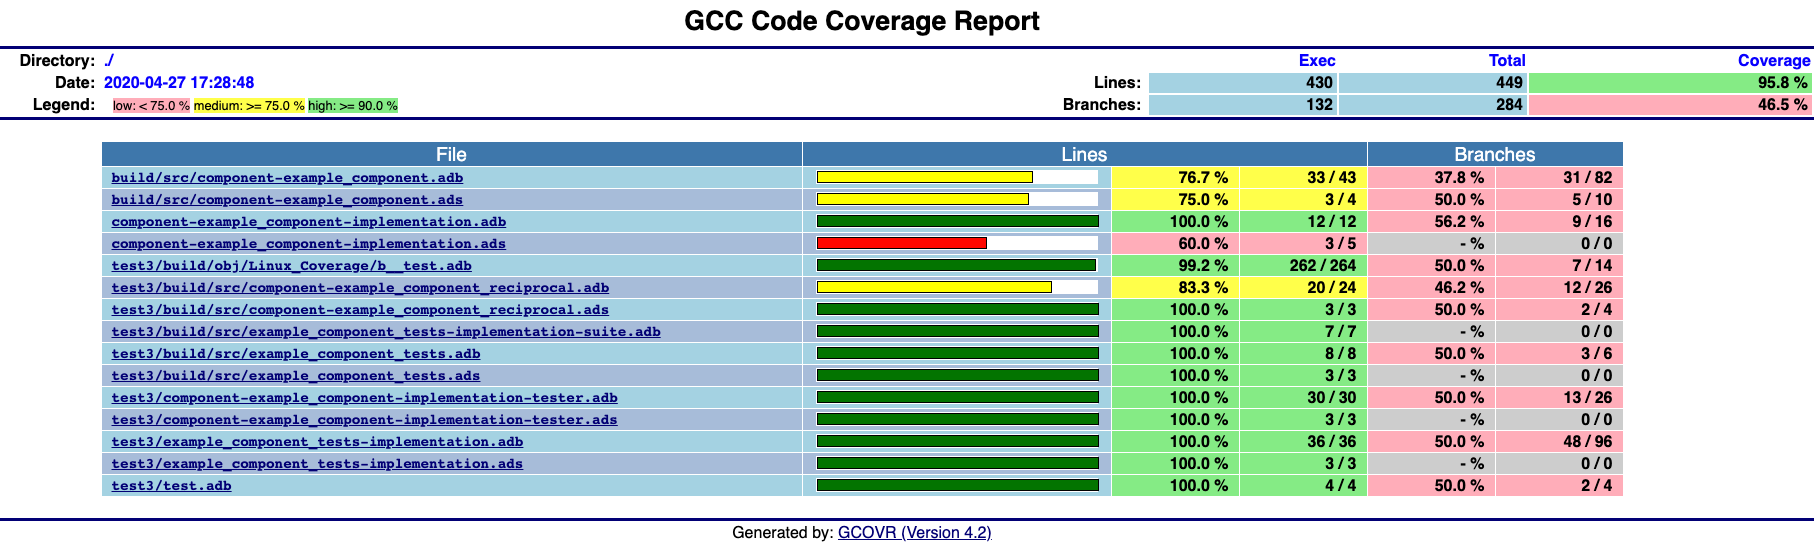
\includegraphics[width=\textwidth]{images/gcovr_component_1.png}
\vspace{5mm} %5mm vertical space

\textit{Specific File Page:}

\vspace{5mm} %5mm vertical space
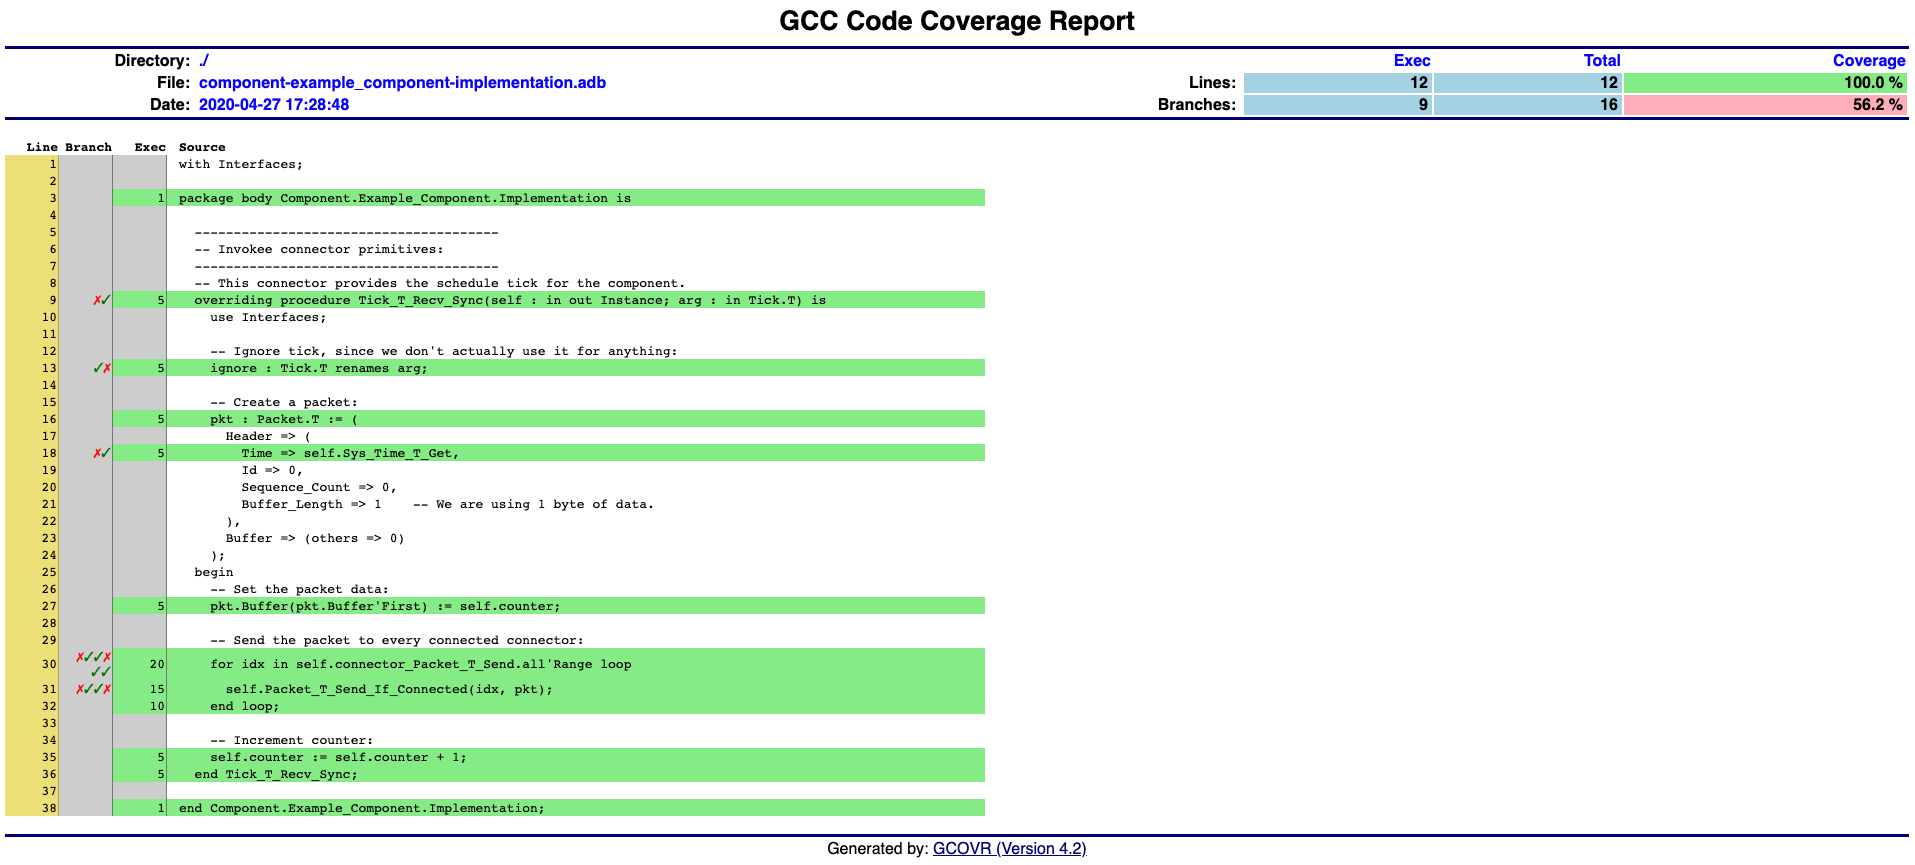
\includegraphics[width=\textwidth]{images/gcovr_component_2.png}
\vspace{5mm} %5mm vertical space

\subsubsection{Unit Test Documentation}

Creating unit test documentation for component unit tests is the same as creating documentation for ordinary modeled unit tests, see Section \ref{Unit Test Documentation}. The procedure will be repeated below with the \textit{example\_component} unit test for clarity. \\

Adamant provides automatic generation of documentation for any unit test model, including unit tests for components. Currently two versions of documentation can be created: HTML, which is useful for presentation in meetings or for quick reference, and PDF (via \LaTeX), which is useful for formal documentation. \\

To build HTML documentation run:

\vspace{5mm} %5mm vertical space
\begin{minted}{text}
> redo build/html/example_component_tests.html
\end{minted}
\vspace{5mm} %5mm vertical space

which when opened with your favorite web browser looks something like this: \\

\vspace{5mm} %5mm vertical space
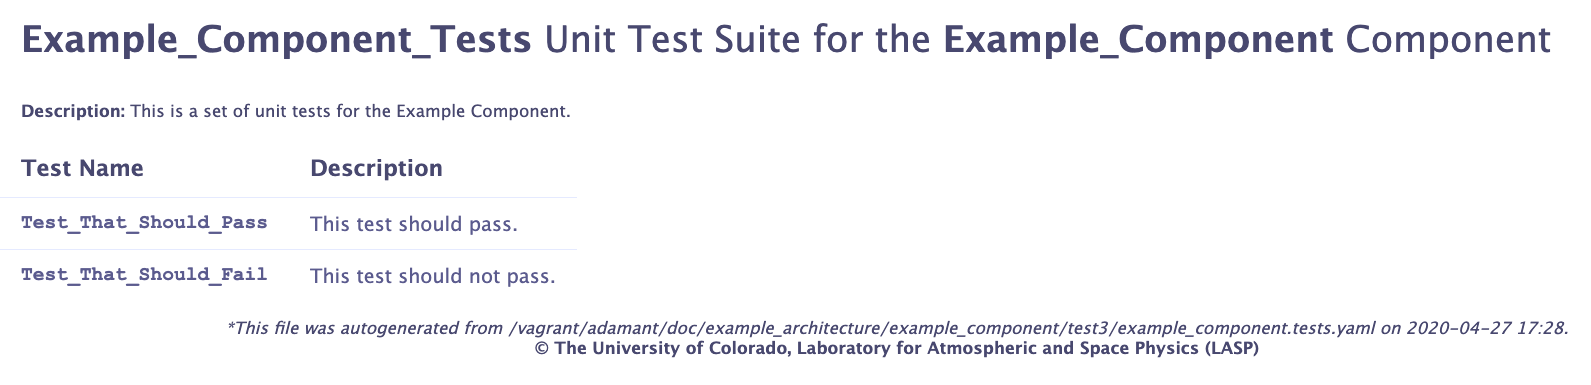
\includegraphics[width=\textwidth]{images/ut_component_html.png}
\vspace{5mm} %5mm vertical space

To build the PDF documentation run:

\vspace{5mm} %5mm vertical space
\begin{minted}{text}
> redo build/pdf/example_component_tests.pdf
\end{minted}
\vspace{5mm} %5mm vertical space

Which produces a PDF output that looks like the following. \\

\noindent\makebox[\linewidth]{\rule{\textwidth}{0.4pt}}
\input{../example_architecture/example_component/test3/build/tex/example_component_tests.tex}
\noindent\makebox[\linewidth]{\rule{\textwidth}{0.4pt}}

\subsection{Creating a Queued Component} \label{Creating a Queued Component}

This section shows an example of building and unit testing a component with an asynchronous connector, which requires an internal queue be instantiated within the component. This section will highlight the differences in working with a component of this type compared to working with a simple passive component, presented in Section \ref{Creating a Passive Component}. It is expected that you understand the concepts presented in that section before reading this section, as the details presented there will not be repeated here. \\


\subsubsection{The Component Queue} \label{The Component Queue}

In Adamant, a component is defined by declaring its interface in a component model, which consists of a list of connectors. If any of these connectors are of kind \texttt{recv\_async} then the component is constructed with an internal queue to store messages for processing at a later time.  \\

In some situations, asynchronous communication might be advantageous. Consider a component whose task is to log data to disk. In order to allow other components to send data to this logger component without waiting for the entire disk write operation to complete (which might be very slow), an asynchronous connection might be used in order to queue the data in memory. In this way, messages sent from components to the logger component will be immediately queued up, allowing those components to continue their normal operation without waiting for the disk write to complete. When the logger executes at some later time (most likely at a lower priority), it will be able to store these messages to disk. \\

A queued component is any component that has one or more asynchronous invoker connectors. If an Adamant component contains at least one asynchronous invoker connector than a single internal queue is instantiated within the component. This queue is generic and can hold items of many different types. If a component contains multiple asynchronous connectors, all of these items are still enqueued on the same single internal queue. Using a single queue makes makes the execution logic of a component simple to understand and implement. When a component ``pops" and item off the queue, a label is included that tell the component which asynchronous connector the item is associated with. Using the label, the component autocode can then call the correct invokee handler procedure to process the connector call. \\

The standard Adamant component queue package can be found \textit{src/data\_structures/labeled\_queue/}. The queue itself is allocated as an array of bytes on the heap. The length of the queue (in bytes) is determined at component initialization and is specified in the assembly model. Each item put on the queue takes up 5 bytes of additional overhead to store the length of the item enqueued and a label which specifies the type of the item, ie. which asynchronous connector the data belongs to. The component queue is implemented as an Ada \textit{protected object}. This means that access to the queue by multiple tasks in the system is safe and free from corruption. Because of this the queue can also be used for task synchronization, as will be shown in Section \ref{Creating an Active Component}. \\

Note that Adamant also offers a priority queue as an alternative to the standard queue for when dequeuing items in first-in-first-out (FIFO) order is not sufficient. Creating a component with a priority queue is discussed in Section \ref{Implementing a Priority Queued Component}. \\

In the following section we create a component with an internal queue and demonstrate how it is used.

\subsubsection{Implementing a Queued Component} \label{Implementing a Queued Component}

In this section we will still be working with a passive component, that is a component without a thread of execution. This means that the component will still only act on the thread of it's connector invokers. In this case, a synchronous connector must be used to service any connector calls that have been queued. This design is ideal for components that need to execute at a very specific time, say on a periodic rate group, but can receive work to do asynchronously. \\

Let's create a new component called \textit{queued\_component} in a new directory.

\vspace{5mm} %5mm vertical space
\begin{minted}{text}
> mkdir queued_component   # make component directory
> cd queued_component 
> touch .all_path          # add directory to build path
\end{minted}
\vspace{5mm} %5mm vertical space

To define the component in this directory, we create a YAML model file \textit{queued\_component.component.yaml} with the following contents. \\

\textit{queued\_component.component.yaml}
\yamlcodef{../example_architecture/queued_component/queued_component.component.yaml}

This model file generates the following component diagram. See Section \ref{Creating a Component Diagram} for directions on how to create a component diagram.

\vspace{5mm} %5mm vertical space
\includegraphics[width=1.0\textwidth,center]{../example_architecture/queued_component/build/eps/queued_component.eps}
\caption{A queued component which has two asynchronous connectors.}
\vspace{5mm} %5mm vertical space

We want this component to be similar to the \textit{example\_component} we constructed in the previous sections. It will still produce a timestamped packet every time a \texttt{Tick.T} is received. However, this time, the contents of the packet will be set asynchronously by one of two asynchronous connectors. The first asynchronous connector will contain an 8-bit value that will get enqueued, the second a 16-bit value. In either case, when the data is received, the packets produced on the \texttt{Tick.T} will hold a copy of the last received data, and the packet length will be set to 1 or 2 bytes accordingly. \\

First let's take a look at the component base package so that we can see the component's internal queue. The base package can autocoded and compiled with the following command.

\vspace{5mm} %5mm vertical space
\begin{minted}{text}
> redo build/obj/Linux/component-queued_component.o
\end{minted}
\vspace{5mm} %5mm vertical space

This should generate and compile two files \textit{build/src/component-queued\_component.ads} and \textit{build/src/component-queued\_component.adb}. Let's take a look the specification. \\

\textit{component-queued\_component.ads}:
\adacodef{../example_architecture/queued_component/build/src/component-queued_component.ads}

This look very similar to the \textit{example\_component} base package that is presented in Section \ref{Component Base Package}. The differences are discussed below. \\

First, take note of some public subprograms that were generated: \texttt{Get\_Max\_Queue\_Element\_Size}, \texttt{Get\_Queue\_Current\_Percent\_Used}, and \texttt{Get\_Queue\_Maximum\_Percent\_Used}. These public functions are meant to be used by the assembly and the Queue Monitor component that is included as part of Adamant. They should not be called within the component and so will not be discussed further here. \\

Also defined in the public section is \texttt{Init\_Base} and \texttt{Final\_Base} procedures. These subprograms are responsible for allocating the queue on the heap, and deallocating it. Note that the parameter to set the queue size specifies the size in bytes. The \texttt{Init\_Base} procedure is called by the assembly during initialization of the component. See Section \ref{Component Base Initialization} for more details on this subprogram. \\

Next, let's take a look at the private section. There is a new enumeration type declared called \texttt{Connector\_Identifier\_Type}, which contains an enumeration literal for each of the asynchronous connectors in our component and a special \texttt{Quit} enumeration. This type is the \texttt{queue label}, and will be used to determine the type of object enqueued on the component's queue. \\

The next code of note are the two private subprograms \texttt{dispatch\_n} and \texttt{dispatch\_all}. These procedures ``dispatch" N items off the queue, or drain the queue respectively. When an item is dispatched, it is removed from the queue, the label is inspected, and the correct connector handler procedure is called to process the queued item. These procedures are meant to be called within a queued, passive component to specify when the component should process any asynchronous items that it received. If these procedures are never called, then the queue will never be serviced, and the component will never act on any asynchronous calls, so they MUST be used within the component. These subprograms are not necessary in an queued, active component, as is discussed in Section \ref{Creating an Active Component}. \\

Finally, if we look at the private component record definition we can see a new variable \texttt{queue} which is the actual queue object instantiated within the component. The type of the queue is \texttt{Queue\_Package.Instance} which is a result of a generic instantiation of the Adamant \texttt{Labeled\_Queue} type, seen in the private section. Note that the \texttt{queue} object itself should rarely need to be accessed from within the component hand-code, as the only interaction with the object is usually through the \texttt{dispatch\_n} and \texttt{dispatch\_all} procedures discussed in the previous paragraph.

OK, now it is time to hand-code the implementation for this component. As with the \texttt{example\_component} we will first build the templates and copy them into our component directory.

\vspace{5mm} %5mm vertical space
\begin{minted}{text}
> redo build/template/component-queued_component-implementation.ads 
> redo build/template/component-queued_component-implementation.adb 
> cp build/template/* .   # copy templates into component dir
\end{minted}
\vspace{5mm} %5mm vertical space

Next, we modify the templates to include the component's behavior. Below is the specification of the \textit{queued component} implementation package. \\

\textit{component-queued\_component-implementation.ads}:
\adacodef{../example_architecture/queued_component/component-queued_component-implementation.ads}

The only modification made to this file from the template was to add two variable to the component record: \texttt{data\_Length} which holds the length of data that will be used in the emitted packet, and \texttt{data} which is the actual data that will be used in the emitted packet. These variables will be set within the two asynchronous connector handlers, as seen in the body. \\

\textit{component-queued\_component-implementation.adb}:
\adacodef{../example_architecture/queued_component/component-queued_component-implementation.adb}

The first subprogram we should look at here is the \texttt{Tick\_T\_Recv\_Sync} procedure that gets invoked when the \texttt{Tick\_T\_Recv\_Sync} connector is called. When a \texttt{Tick.T} is received, the component first calls the \texttt{Self.Dispatch\_All} function that is implemented in the component base package. Recall that this function will drain the component's internal queue, calling the correct connector handlers for each item dequeued. Specifically, this procedure will take items off the queue and call either the \texttt{Packed\_Byte\_T\_Recv\_Async} procedure or the \texttt{Packed\_U16\_T\_Recv\_Async} procedure depending on the type of the popped item. Next, a packet is created and sent out. The length of the packet is determined by the \texttt{Self.Data\_Length} variable and the contents by the \texttt{data} variable. \\

Next, there are two subprograms \texttt{Packed\_Byte\_T\_Recv\_Async} and \texttt{Packed\_U16\_T\_Recv\_Async}. These procedures are the asynchronous connector handlers that will be invoked when \texttt{Self.Dispatch\_All} or \texttt{Self.Dispatch\_N} is called. They both perform similar actions, saving off the received data and data length into the component's internal variables for later packetization. \\

Finally, there are two subprograms \texttt{Packed\_Byte\_T\_Recv\_Async\_Dropped} and \texttt{Packed\_U16\_T\_Recv\_Async\_Dropped}. These procedures will be called by the autocoded base package whenever the \texttt{Packed\_Byte\_T\_Recv\_Async} or \texttt{Packed\_U16\_T\_Recv\_Async} connectors is invoked, but the internal queue is full. In this case, the data is dropped, the connector handler is not called, and, instead, the \texttt{*\_Dropped} procedure is called. This functionality allows a component to perform some action when the internal queue overflows. Normally you will want to code some intelligent behavior here, but for simplicity the code above just produces a fail print using \texttt{Ada.Text\_IO}. \\

Note that this design is completely thread safe, assuming only a single task calls the \texttt{Tick\_T\_Recv\_Sync} connector, which is the intended use. The internal queue is used as a synchronization mechanism. Data can be enqueued by multiple tasks simulaneously. Data is dequeued by the task that calls \texttt{Tick\_T\_Recv\_Sync} connector, processed, and then emitted as a packet on the same task. \\

We can make sure that this code compiles by running:

\vspace{5mm} %5mm vertical space
\begin{minted}{text}
> redo build/obj/Linux/component-queued_component-implementation.o
\end{minted}
\vspace{5mm} %5mm vertical space

or by simply running \texttt{redo all}. \\

In the next section we will unit test this component.

\subsubsection{Unit Testing a Queued Component} \label{Unit Testing a Queued Component}

In this section we will create a unit test model to assist in unit testing the \textit{queued\_component}. This section will not discuss the details of unit testing a component. It will only highlight the differences in unit testing a queued component as compared to a passive component. You should be familiar with the concepts presented in Section \ref{Component Unit Testing} before reading this section. \\

To start, we create a unit test directory called \textit{test/} under our component directory:

\vspace{5mm} %5mm vertical space
\begin{minted}{text}
> mkdir test  # Make test/ within queued_component/
> cd test
\end{minted}
\vspace{5mm} %5mm vertical space

Next, we are going to create a component unit test model file \textit{queued\_component.tests.yaml}. The contents are shown below:

\yamlcodef{../example_architecture/queued_component/test/queued_component.tests.yaml}

We define two unit tests, one that tests the nominal execution of the component, sending it \texttt{Tick.T}s and expecting packets to be produced, the other testing the behavior when the component's internal queue becomes full. \\

We also need to add an \textit{env.py} file to this directory as we did in Section \ref{Component Unit Testing} to make sure we are using the \texttt{Linux\_Test} target. \\

Next, we can generate the unit test templates and copy them into the test directory.

\vspace{5mm} %5mm vertical space
\begin{minted}{text}
> redo build/template/component-queued_component-implementation-tester.ads
> redo build/template/component-queued_component-implementation-tester.adb
> redo build/template/queued_component_tests-implementation.ads
> redo build/template/queued_component_tests-implementation.adb
> redo build/template/test.adb
> cp build/template/* .  # copy the template files into test/
\end{minted}
\vspace{5mm} %5mm vertical space

Now the unit tests can be implemented by editing \textit{queued\_component\_tests-implementation.adb}. The implemented unit tests are shown below. \\

\textit{queued\_component\_tests-implementation.adb}:
\adacodef{../example_architecture/queued_component/test/queued_component_tests-implementation.adb}

The first unit test sends some data to the component through the asynchronous connectors. It then sends a tick and makes sure a packet is produced with the correct output data. \\

The second unit test simply fills the component queue. Note that queue size is set in the \texttt{Set\_Up\_Test} fixture to 3 times the maximum queue element size. In this case, the maximum queue element would correspond to enqueueing a \texttt{Packed\_U16} type. This is achieved by calling \texttt{Self.Tester.Packed\_U16\_T\_Send} 4 times. The fourth call should overflow the queue. \\

The unit test can be compiled and run using the command:

\vspace{5mm} %5mm vertical space
\begin{minted}{text}
> redo test
\end{minted}
\vspace{5mm} %5mm vertical space

which produces the output

\vspace{5mm} %5mm vertical space
\inputminted{text}{../example_architecture/queued_component/test/output.txt}
\vspace{5mm} %5mm vertical space

As can be seen, the component's \texttt{*\_Dropped} handler was called because the ``\texttt{Oh no! The queue overflowed!}" message is printed. We can also see that the second unit test failed with an assertion. This assertion is being triggered inside of the tester component, which throws an assertion if it ever detects that the internal component's queue overflowed. This is the default behavior to preventing the accidental overflowing of a queue during unit test. \\

There are times, however, when we actually \textit{want} to overflow a queue during unit test to test that specific behavior. In this case, we can modify the unit test as follows. \\

\textit{queued\_component\_tests-implementation.adb}:
\adacodef{../example_architecture/queued_component/test2/queued_component_tests-implementation.adb}

In this case, we have added the line \texttt{Self.Tester.Sxpect\_Packed\_U16\_T\_Send\_Dropped := True;} which tells the tester component that the next connector call will overflow the queue. When this is set, the component will not throw an assertion. See the new output below.

\vspace{5mm} %5mm vertical space
\inputminted{text}{../example_architecture/queued_component/test2/output.txt}
\vspace{5mm} %5mm vertical space

Note that any subsequent call that may overflow the queue will trigger the assertion again. The \texttt{Self.Tester.Expect\_Packed\_U16\_T\_Send\_Dropped} variable must be set before every call to a connector that will be dropped. In this way, the tester component will always alert the developer if something was dropped off a queue during unit test that was not intended. 

\subsubsection{Implementing a Priority Queued Component} \label{Implementing a Priority Queued Component}

The previous sections presented how to construct and unit test a component that contains a standard internal queue. The Adamant standard queue is a very efficient (in both space and time) first-in-first-out FIFO queue. However, sometimes it is desirable to have a queue that implements priority-based dequeueing logic instead of FIFO. Priority queues allow the component to process messages deemed more important prior to servicing others, regardless of the order in which they were enqueued. \\

A few implementation differences between the Adamant standard queue and the priority queue should be understood. The standard queue is implemented as a single buffer of memory where queued items are stored efficiently, packed together, with no wasted bytes. As such, initializing the standard queue requires that the user specify the total number of bytes the queue should contain. The priority queue does not make as efficient use of memory. Each element on the priority queue takes up the number of bytes necessary to hold the maximum sized element that the queue will need to hold. So if two different types need to be stored on the queue, one takes up 5 bytes and another takes up 500 bytes, each element on the queue will be 500 bytes in length. Enqueuing the 5 byte item will leave 495 bytes unused in that queue entry. Instead of initializing the queue as a total number of bytes, a priority queue is initialized with a \textit{depth} which specifies how many entries of maximum size the queue will hold before beginning to drop items. \\

A priority queue is also less efficient in terms of performance than a standard Adamant queue. The standard queue has a complexity of \textit{O(1)} queue and dequeue execution times. The priority queue is slower, taking \textit{O(log n)} queue and dequeue where \textit{n} is the number of items currently stored on the queue. \\

With this in mind, priority queues should only be used where servicing items based on priority is essential, and that benefit outweighs the performance hits in both time and space. If you are still convinced you need to implement a component with a priority queue, continue on. \\

Adamant provides priority queueing for a component if a \texttt{priority} is specified for a \texttt{recv\_async} connector. For example, we can instantiate the \textit{queued\_component} presented in the previous sections with an internal priority queue by defining \texttt{priorities} for each of the two \texttt{recv\_async} connectors. Let's call it \textit{priority\_queued\_component}. \\

\textit{priority\_queued\_component.component.yaml}
\yamlcodef{../example_architecture/priority_queued_component/priority_queued_component.component.yaml}

You can that a priority of 1 has been specified for the \texttt{Packed\_Byte\_T\_Recv\_Async} connector and a priority of 2 has been specified for the \texttt{Packed\_U16\_T\_Recv\_Async} connector. Connector's of higher numeric valued priorities will be serviced before connectors of lower numeric valued priorities. So in this case if both an \texttt{Packed\_U16\_T\_Recv\_Async} and a \texttt{Packed\_Byte\_T\_Recv\_Async} item are put on the queue, the \texttt{Packed\_U16\_T\_Recv\_Async} item will be dequeued first, no matter the order in which the items were enqueued. \\

The connector \texttt{priority} can be any integer value between 0 and 255, inclusive. Connectors with an identical priority value will have their enqueued items serviced in FIFO order. Note that if not specified, the priority for a \texttt{recv\_async} connector is assumed to be 0. If all connectors have the same priority, the component is instantiated with a standard Adamant queue instead of a priority queue. Specifying \texttt{priority} for a connector not of kind \texttt{recv\_async} is considered illegal and will produce a modeling error. \\

The model file above generates the following component diagram. See Section \ref{Creating a Component Diagram} for directions on how to create a component diagram.

\vspace{5mm} %5mm vertical space
\includegraphics[width=1.0\textwidth,center]{../example_architecture/priority_queued_component/build/eps/priority_queued_component.eps}
\caption{A priority queued component which has two asynchronous connectors of different priority.}
\vspace{5mm} %5mm vertical space

You can see how the priorities of each \texttt{recv\_async} connector is now visible in the diagram. \\

Implementing and unit testing a component with a priority queue is no different than implementing a component with a standard queue. You just have to remember that the \texttt{recv\_async} connector handlers will be called in the order of the priority of the items enqueued, and not in FIFO order. \\

\subsection{Creating an Active Component} \label{Creating an Active Component}

In this section we will be working with an \textit{active} component, that is, a component with a thread of execution, or a \textit{task} allocated to it. This means that the component will run whenever the task becomes ready to run and no other higher priority tasks are running. The Ada scheduler manages the running of active tasks based on their priority. More details on the component task are provided in the next section.

\subsubsection{The Component Task}  \label{The Component Task}

A component is considered ``active" in Adamant when it is provided a task of execution. This is done by specifying the component \textit{execution} as ``active" in the component model, as will be seen in the following section. When a component is defined active, the assembly must instantiate a task for that component during initialization. The definition of this task is the same for any active component, and is defined in the Adamant component core package in \textit{src/core/component/}. To better understand what a component task looks the specification of the component package is shown below. \\

\textit{component.ads}:
\adacodef{../../src/core/component/component.ads}

There are a lot of low level details here that we don't need to get into, however, there are a few things to note. First look at the abstract procedure \texttt{Cycle}. This abstract subprogram must be overridden by an inheriting type in order to specify the behavior that the component will perform on each ``cycle" of the task. This subprogram is called inside the task definition for \texttt{Active\_Task}. \\

We can see that \texttt{Active\_Task} takes many parameters in its discriminant including vital task information such as the priority and stack size. To fully understand what happens in a component task we need to look at the body. \\

\textit{component.adb}:
\adacodef{../../src/core/component/component.adb}

If we look at \texttt{task body Active\_Task} we can see that it enters an infinite loop where it calls \texttt{Cycle} repeatedly. The \texttt{Cycle} procedure does all the work in this case, and must be defined by an inheriting type. \\

As you can imagine, a programmer can override the \texttt{Cycle} program and code their own custom logic to perform on a component's task. This is demonstrated in Section \ref{Creating a Background Component}. However, in Adamant systems, this is rarely, if ever, done. The most common pattern is to use an active component in tandem with a component's internal queue to define the execution of the component. By default, if a component is both active and has at least one asynchronous connector, the \texttt{Cycle} procedure gets defined in the component's base package with the following behavior. \\

\vspace{5mm} %5mm vertical space
\begin{spacedenumerate}
  \item The component task ``blocks" (waits) on queue until it is no longer empty.
  \item When an item is placed on the queue the component becomes ready to run. When there are no higher priority tasks running, the scheduler will run this task.
  \item The component pops an item off the queue and then processes it by calling the appropriate asynchronous connector handler procedure.
  \item Go back to step 1.
\end{spacedenumerate}
\vspace{5mm} %5mm vertical space

In this way, the execution of the component is metered by the work it needs to do. The work it does is determined by the items that are put on its queue, which are processed serially. In this case, the queue acts as a synchronization mechanism, providing thread safety for the active component's execution by ordering the component processing in a FIFO manner. The processing of each item is completed before the next item is popped off the queue. \\

In the following section a component is constructed using this pattern.

\subsubsection{Implementing an Active Component}

Let's create a new component called \textit{active\_component} in a new directory.

\vspace{5mm} %5mm vertical space
\begin{minted}{text}
> mkdir active_component   # make component directory
> cd active_component 
> touch .all_path          # add directory to build path
\end{minted}
\vspace{5mm} %5mm vertical space

To define the component in this directory, we create a YAML model file \textit{active\_component.component.yaml} with the following contents. \\

\textit{active\_component.component.yaml}
\yamlcodef{../example_architecture/active_component/active_component.component.yaml}

This model file generates the following component diagram. See Section \ref{Creating a Component Diagram} for directions on how to create a component diagram.

\vspace{5mm} %5mm vertical space
\includegraphics[width=1.0\textwidth,center]{../example_architecture/active_component/build/eps/active_component.eps}
\caption{An active component which has two asynchronous connectors.}
\vspace{5mm} %5mm vertical space

We want this component to be similar to the \textit{queued\_component} we constructed in the previous sections. It will still produce a timestamped packet based on input data from two asynchronous connectors. However, this time, there is no \texttt{Tick.T} connector that drives the component's execution. Instead, the component is made active, and so will produce a packet any time data is put on its internal queue. \\

First let's take a look at the component base package so that we can see the component's definition of the \texttt{Cycle} procedure. The base package can autocoded and compiled with the following command.

\vspace{5mm} %5mm vertical space
\begin{minted}{text}
> redo build/obj/Linux/component-active_component.o
\end{minted}
\vspace{5mm} %5mm vertical space

This should generate and compile two files \textit{build/src/component-active\_component.ads} and \textit{build/src/component-active\_component.adb}. The specification and body are not shown here because they are quite large. However the reader is encouraged to inspect them to see that the \texttt{Cycle} procedure is indeed implemented with the logic described in the previous section. \\

OK, now it is time to hand-code the implementation for this component. As with the \texttt{example\_component} we will first build the templates and copy them into our component directory.

\vspace{5mm} %5mm vertical space
\begin{minted}{text}
> redo build/template/component-active_component-implementation.ads 
> redo build/template/component-active_component-implementation.adb 
> cp build/template/* .   # copy templates into component dir
\end{minted}
\vspace{5mm} %5mm vertical space

Next, we modify the templates to include the component's behavior. To implement this component, no modifications were made to the specification. In particular, this component defines no variables in the component record in the implementation specification. The connector handler behavior is encoded in the implementation body, which is shown below. \\

\textit{component-active\_component-implementation.adb}:
\adacodef{../example_architecture/active_component/component-active_component-implementation.adb}

We can see that the implementations of \texttt{Packed\_Byte\_T\_Recv\_Async} and \texttt{Packed\_U16\_T\_Recv\_Async} are very similar. Any time an item is popped off the component's queue one of these handlers is called. A packet is then created containing the data item and sent out of the component. The \texttt{Packed\_Byte\_T\_Recv\_Async\_Dropped} and \texttt{Packed\_U16\_T\_Recv\_Async\_Dropped} subprograms are implemented in the same fashion as in Section \ref{Implementing a Queued Component} and will get called if the component queue ever becomes too full to hold another item. \\

We can make sure that this code compiles by running:

\vspace{5mm} %5mm vertical space
\begin{minted}{text}
> redo build/obj/Linux/component-active_component-implementation.o
\end{minted}
\vspace{5mm} %5mm vertical space

or by simply running \texttt{redo all}. \\

\subsubsection{Unit Testing an Active Component}

In this section we will create a unit test model to assist in unit testing the \textit{active\_component}. This section will not discuss the details of unit testing a component. It will only highlight the differences in unit testing an active component as compared to a queued component. You should be familiar with the concepts presented in Section \ref{Component Unit Testing} before reading this section. \\

To start, we create a unit test directory called \textit{test/} under our component directory:

\vspace{5mm} %5mm vertical space
\begin{minted}{text}
> mkdir test  # Make test/ within active_component/
> cd test
\end{minted}
\vspace{5mm} %5mm vertical space

Next, we are going to create a component unit test model file \textit{active\_component.tests.yaml}. The contents are shown below:

\yamlcodef{../example_architecture/active_component/test/active_component.tests.yaml}

We define two unit tests, one that tests the nominal execution of the component, sending it data items on it's internal queue and expecting packets to be produced, the other testing the behavior when the component's internal queue becomes full. \\

We also need to add an \textit{env.py} file to this directory as we did in Section \ref{Component Unit Testing} to make sure we are using the \texttt{Linux\_Test} target. \\

Next, we can generate the unit test templates and copy them into the test directory.

\vspace{5mm} %5mm vertical space
\begin{minted}{text}
> redo build/template/component-active_component-implementation-tester.ads
> redo build/template/component-active_component-implementation-tester.adb
> redo build/template/active_component_tests-implementation.ads
> redo build/template/active_component_tests-implementation.adb
> redo build/template/test.adb
> cp build/template/* .  # copy the template files into test/
\end{minted}
\vspace{5mm} %5mm vertical space

Now the unit tests can be implemented by editing \textit{active\_component\_tests-implementation.adb}. The implemented unit tests are shown below. \\

\textit{active\_component\_tests-implementation.adb}:
\adacodef{../example_architecture/active_component/test/active_component_tests-implementation.adb}

The first unit test sends some data to the component through the asynchronous connectors. Note, that the act of sending this data to the component does not cause the component to execute, like it might when the component is running in an assembly. Recall that component unit testing in Adamant is single threaded to make the act of unit testing simpler. This means that an active component is not actually given a thread of execution during unit test. This is advantageous because the unit test developer can exactly specify when the component's internal task executes manually. In this way, very fine grain testing can be achieved. \\

To simulate the component's task executing, the tester component is autocoded with the subprograms \texttt{dispatch\_all} and \texttt{dispatch\_n}. Similar to the same-named methods autocoded in the component base package seen in Section \ref{Implementing a Queued Component}, these subprograms will dequeue items off the component's internal queue and process them in the same manner that the \texttt{Cycle} procedure would when a task is allocated. The advantage is that the programmer can call these dispatch functions at the exact moment they want the component to run instead of dealing with the complexities of managing the execution of a multithreaded unit test environment. \\

Shown in the first test, data is passed to the component on its asynchronous connectors. After that a check is made to ensure that no packets were produced by the component yet. Next, the \texttt{dispatch\_all} procedure is called, causing the component to ``execute", draining its queue and performing all associated processing. After this, we expect two packets to have been produced with the correct internal data. This procedure is then repeated to make sure the component behaves properly. \\

The second unit test simply fills the component queue. Note that queue size is set in the \texttt{Set\_Up\_Test} fixture to 3 times the maximum queue element size. In this case, the maximum queue element would correspond to enqueueing a \texttt{Packed\_U16} type. This is achieved by calling \texttt{Self.Tester.Packed\_U16\_T\_Send} 4 times. The fourth call overflows the queue. This test is identical to the second unit test defined in Section \ref{Unit Testing a Queued Component}. \\

The unit test can be compiled and run using the command:

\vspace{5mm} %5mm vertical space
\begin{minted}{text}
> redo test
\end{minted}
\vspace{5mm} %5mm vertical space

which produces the output

\vspace{5mm} %5mm vertical space
\inputminted{text}{../example_architecture/active_component/test/output.txt}
\vspace{5mm} %5mm vertical space

\subsection{Creating a Background Component} \label{Creating a Background Component}

As discussed in the previous section, active components in Adamant almost always have an asynchronous queue which aids in metering the execution of that component. There are a few instances where not having an asynchronous connector makes sense, mostly in the case of the lowest priority background component (ie. memory scrubbing), or a component whose execution is metered internally by sleeping periodically. This section will briefly show a component of this nature and explain how to unit test it.

\subsubsection{Implementing a Background Component} \label{Implementing a Background Component}

Let's create a new component called \textit{background\_component} in a new directory.

\vspace{5mm} %5mm vertical space
\begin{minted}{text}
> mkdir background_component # make component directory
> cd background_component 
> touch .all_path            # add directory to build path
\end{minted}
\vspace{5mm} %5mm vertical space

To define the component in this directory, we create a YAML model file \textit{background\_component.component.yaml} with the following contents. \\

\textit{background\_component.component.yaml}
\yamlcodef{../example_architecture/background_component/background_component.component.yaml}

This model file generates the following component diagram. See Section \ref{Creating a Component Diagram} for directions on how to create a component diagram.

\vspace{5mm} %5mm vertical space
\includegraphics[width=1.0\textwidth,center]{../example_architecture/background_component/build/eps/background_component.eps}
\caption{An active component which has one synchronous connector.}
\vspace{5mm} %5mm vertical space

We want this component to be similar to the \textit{active\_component} we constructed in the previous sections, however it contains no asynchronous connectors. Instead the packet data is received synchronously. A packet is sent out at a period rate, managed internally by the component's task. \\

OK, now it is time to hand-code the implementation for this component. As with the \texttt{example\_component} we will first build the templates and copy them into our component directory.

\vspace{5mm} %5mm vertical space
\begin{minted}{text}
> redo build/template/component-background_component-implementation.ads 
> redo build/template/component-background_component-implementation.adb 
> cp build/template/* .   # copy templates into component dir
\end{minted}
\vspace{5mm} %5mm vertical space

Before we modify the templates, let's take a look at them first. Below is the implementation file. \\

\textit{component-background\_component-implementation.adb}:
\adacodef{../example_architecture/background_component/build/template/component-background_component-implementation.adb}

As can be seen, there is an overriding \texttt{Cycle} procedure. Because there is no asynchronous queue, Adamant does not provide a default implementation of this procedure in the base package autocode. Instead, the programmer is asked to define the task behavior by implementing the \texttt{Cycle} function in the implementation package. By default, the implementation simply fails with an assertion, making sure the developer is quickly alerted if this procedure is not properly implemented. \\

Next, let's modify the templates to include the component's behavior. First, let's look at the specification. \\

\textit{component-background\_component-implementation.ads}:
\adacodef{../example_architecture/background_component/component-background_component-implementation.ads}

The first thing to notice is the definition of the protected type \texttt{Protected\_Data}. This is an Ada entity that provides mutual exclusion to the data members that it protects. In this case, we are building a protected object around a two byte data field that will be used to populate the component's outgoing packet. The protected type provides two methods to access the protected data, a setter and a getter. This data must be protected since many components could call the \textit{background\_component}'s \texttt{Packed\_U16\_T\_Recv\_Sync} connector simultaneously. In addition, the \textit{background\_component} could be reading the data into the packet at the same time it is being set by an external component. To prevent the race condition and data corruption that could occur in these scenarios, the data is protected with a protected type, which ensures mutual exclusion. \\

In the component record, we can see that there is an instance of \texttt{Protected\_Data} called \texttt{p\_Data}. There is also a variable called \texttt{wake\_Up\_Time} which stores the next absolute time that the component should wake up and execute. This variable is initialized to the current time. \\

Now let's take a look at the implementation: \\

\textit{component-background\_component-implementation.adb}:
\adacodef{../example_architecture/background_component/component-background_component-implementation.adb}

First, the \texttt{Protected\_Data} protected type body is shown. Again, these are simple setter and getter subprograms, but because they are protected, provide the necessary thread safety. We can also see the implementation \texttt{Packed\_U16\_T\_Recv\_Async} which simply copies the provided data into the protected object. \\

Next, is the definition of \texttt{Cycle}. Recall that this function will be called indefinitely in a loop by the component's task, see Section \ref{The Component Task}. First this function delays (sleeps) until the wake up time arrives. This allows other tasks the execute while this task is sleeping. When the wake up time arrives, this task will be come ready to run and the scheduler will run it, so long as there are no other higher priority tasks currently running. When given time to execute, the component will then create a packet, copying the protected data into the packet's data field, and then send it out. Finally, the component computes the next wake up time. This execution cycle will repeat forever. \\

At any time during the components execution, an external call to \texttt{Packed\_U16\_T\_Recv\_Async} can change the contents of the data that is produced. There is no fear of data corruption since the shared data has been made protected. \\

We can make sure that this code compiles by running:

\vspace{5mm} %5mm vertical space
\begin{minted}{text}
> redo build/obj/Linux/component-background_component-implementation.o
\end{minted}
\vspace{5mm} %5mm vertical space

or by simply running \texttt{redo all}. \\

\subsubsection{Unit Testing a Background Component}

In this section we will create a unit test model to assist in unit testing the \textit{background\_component}. This section will not discuss the details of unit testing a component. It will only highlight the differences in unit testing a background component as compared to an active or queued component. You should be familiar with the concepts presented in Section \ref{Component Unit Testing} before reading this section. \\

To start, we create a unit test directory called \textit{test/} under our component directory:

\vspace{5mm} %5mm vertical space
\begin{minted}{text}
> mkdir test  # Make test/ within background_component/
> cd test
\end{minted}
\vspace{5mm} %5mm vertical space

Next, we are going to create a component unit test model file \textit{background\_component.tests.yaml}. The contents are shown below:

\yamlcodef{../example_architecture/background_component/test/background_component.tests.yaml}

We define a single unit test that runs the component through a nominal scenario. \\

We also need to add an \textit{env.py} file to this directory as we did in Section \ref{Component Unit Testing} to make sure we are using the \texttt{Linux\_Test} target. \\

Next, we can generate the unit test templates and copy them into the test directory.

\vspace{5mm} %5mm vertical space
\begin{minted}{text}
> redo build/template/component-background_component-implementation-tester.ads
> redo build/template/component-background_component-implementation-tester.adb
> redo build/template/background_component_tests-implementation.ads
> redo build/template/background_component_tests-implementation.adb
> redo build/template/test.adb
> cp build/template/* .  # copy the template files into test/
\end{minted}
\vspace{5mm} %5mm vertical space

Now the unit tests can be implemented by editing \textit{background\_component\_tests-implementation.adb}. The implemented unit tests are shown below. \\

\textit{background\_component\_tests-implementation.adb}:
\adacodef{../example_architecture/background_component/test/background_component_tests-implementation.adb}

The unit test sends some data to the component through its synchronous receive connector. Note, that the act of sending this data to the component does not cause the component to execute. The component can only execute when its \texttt{Cycle} procedure is called. Recall that component unit testing in Adamant is single threaded to make the act of unit testing simpler. This means that an active component is not actually given a thread of execution during unit test. This is advantageous because the unit test developer can exactly specify when the component's internal task executes manually. In this way, very fine grain testing can be achieved. \\

To simulate the component's task executing, the tester component is autocoded with the subprogram \texttt{Cycle\_Component} which calls the component's \texttt{Cycle} procedure directly, simulating the running of the task. The advantage is that the programmer can call this \texttt{Cycle\_Component} procedure at the exact moment they want the component to run instead of dealing with the complexities of managing the execution of a multithreaded unit test environment. \\

Shown in the test, data is passed to the component on its synchronous connector. After that a check is made to ensure that no packets were produced by the component yet. Next, the \texttt{Cycle\_Component} procedure is called, causing the component to ``execute" which causes a single packet to be produced. The unit test ensures that the packet's data is correct and then repeats the procedure again, ensuring that a packet is produced for each call to \texttt{Cycle\_Component}. \\

The unit test can be compiled and run using the command:

\vspace{5mm} %5mm vertical space
\begin{minted}{text}
> redo test
\end{minted}
\vspace{5mm} %5mm vertical space

which produces the output

\vspace{5mm} %5mm vertical space
\inputminted{text}{../example_architecture/background_component/test/output.txt}
\vspace{5mm} %5mm vertical space

\subsection{Protected Objects within Components}

Ada uses \textit{protected objects} to provide mutual exclusion and task synchronization for multi-tasked systems. In Adamant, protected objects should be used within a component to protect shared data that could be accessed simultaneously by more than a single task. Protected objects should ALWAYS be used in this case, even if the shared data is a single byte or a single word that you assume is atomically updated. The only way to ensure mutual exclusion and produce platform independent code is to use protected objects. The implementation of protected objects is via code insertion by the compiler, and thus is very performant. One should not hesitate to employ the use of a protected object when it is required. \\

The following component patterns require the use of a protected object:

\vspace{5mm} %5mm vertical space
\begin{spaceditemize}
  \item A component has a connector of kind \texttt{recv\_sync} that can be called by multiple outside components. Any internal data that is updated in this connector handler must be made protected.
  \item A component has a connector of kind \texttt{recv\_sync} that writes to data that could be read by the component on another thread of execution. This shared data must be made protected.
  \item A component has a connector of kind \texttt{return} or \texttt{modify} that returns data that could be written to on another thread of execution. This shared data must be made protected.
\end{spaceditemize}
\vspace{5mm} %5mm vertical space

The use of protected objects within Adamant components is not as common as might be assumed by the list above. The Adamant internal queue is itself a protected object. The use of \texttt{recv\_async} connectors can often bypass the need to create a user-defined protected object. For more information on the component queue see Section \ref{The Component Queue}. \\

It should also be noted that user-defined protected objects are never used for task synchronization within Adamant. Adamant component queues provide the sole mechanism for task synchronization. This keeps the execution and interaction of components easy to understand by simply looking at component diagrams. \\

An example of defining and using a protected object within a component is presented in Section \ref{Implementing a Background Component}.

\subsection{Component Initialization} \label{Component Initialization}

Components in Adamant get initialized in phases. The initialization of components within in each phase is order independent, however the ordering of each phase itself is important. Component initialization is provided by assembly level autocode, however, what gets initialized within each component is defined by each component's model. The different phases of component initialization are summarized below.

\vspace{5mm} %5mm vertical space
\begin{spacedenumerate}
  \item \textbf{Component Instantiation} - Every component is instantiated from a component type. Components may specify a \textit{discriminant} in their component models to specify parameters to be used during instantiation.
  \item \textbf{Component Base Initialization} - A \texttt{Init\_Base} procedure is autocoded for any component that requires heap allocation for base package objects. This includes queues and unconstrained arrayed connectors.
  \item \textbf{Component Set ID Bases} - A \texttt{Set\_Id\_Bases} procedure is autocoded for any component that includes an IDed Entity Suite, see Section \ref{Component IDed Entities}. This procedure is used to set the base ID for each entity suite.
  \item \textbf{Component Implementation Initialization} - Components may specify an \texttt{Init} procedure with custom parameters in their model. This procedure is called in order to initialize any implementation package variables. This can include allocations on the heap, saving off input parameters, etc.
  \item \textbf{Component Set Up} - Components are not allowed to make connector calls during any of the initialization phases described above, since it is not safe to assume that an invoked component has completed its initialization. A \texttt{Set\_Up} procedure is provided for all components in order to provide a safe initialization phase to call connectors. By default, the implementation of this method is \texttt{null}, however it is commonly overridden to publish data products at startup or other perform other connector invocations that must occur at boot.
\end{spacedenumerate}
\vspace{5mm} %5mm vertical space

The following sections will go into detail on each of the initialization phases and provide an example component that demonstrates each feature.

\subsubsection{Component Instantiation} \label{Component Instantiation}

By default, every component is initialized without parameters. Parameters may be provided at instantiation using the \textit{discriminant}. The \textit{discriminant} is an Ada language feature that allows parameterization of a record type. \\

Not all Ada types can be supplied as a discriminant parameter, and the list is even more restricted when using the Ravenscar profile. However, in Adamant, discriminants are commonly used to provide static values such as task priorities or interrupt identifiers. It is also common to pass access types to data that parameterize the behavior of the component. Note that lengths cannot be passed into the discriminant and used to size an array (or other such operations) as this causes implicit heap allocation, which is forbidden by the Ravenscar profile. Parameters included in the discriminant can be accessed in component implementation code just like any other field of the \texttt{Instance} record. \\ 

A discriminant can be defined in a component model as follows: \\

\textit{discriminated\_component.component.yaml}
\yamlcodef{../example_architecture/discriminated_component/discriminated_component.component.yaml}

In this model we define the component's discriminant with the \texttt{discriminant} tag. Note that all fields are commented to indicate whether they are \textit{required} or \textit{optional}. \\

This component is discriminated with two parameters, \texttt{Packets\_Per\_Tick}, which specifies the number of packets the component produces every time it receives a \texttt{Tick.T}, and \texttt{Enabled\_At\_Startup}, which defines whether or not the component produces packets at all when first initialized. \\

Let's take a look at how this model is reflected in the component autocode. We generate the component template specification file with the following commands:

\vspace{5mm} %5mm vertical space
\begin{minted}{text}
> redo build/template/component-discriminated_component-implementation.ads
> cp build/template/* .   # copy template into component dir
\end{minted}
\vspace{5mm} %5mm vertical space

Here is what the specification file looks like: \\

\textit{component-discriminated\_component-implementation.ads}:
\adacodef{../example_architecture/discriminated_component/build/template/component-discriminated_component-implementation.ads}

Notice the definition of the component record \texttt{Instance} now includes the two discriminant parameters \texttt{Packets\_Per\_Tick} and \texttt{Snabled\_At\_Startup}. To instantiate the component these parameters now must be provided. This is done in an Adamant assembly model, but the autocode that instantiates the component would look something like this:

\vspace{5mm} %5mm vertical space
\begin{adacode}
  Discriminated_Component_Instance := Component.Discriminated_Component.Instance (
    Packets_Per_Tick => 3,
    Enabled_At_Startup => True
  );
\end{adacode}
\vspace{5mm} %5mm vertical space

Note that the discriminant parameters can be accessed inside of the component implementation package by simply referencing them via \texttt{Self.Packets\_Per\_Tick} or \texttt{Self.Enabled\_At\_Startup}, as if they were normal record fields. \\

Similar functionality to a discriminant can be provided with the implementation package \texttt{Init} function discussed in Section \ref{Component Implementation Initialization}. You should use an \texttt{Init} function instead of a discriminant if you need to use the parameters to allocate memory on the heap or provide additional computation at startup. Using the discriminant should be considered when a variable is so essential to the functioning of a component that it is required for the component to even be instantiated. One good example of this case is an interrupt handling component, which could not function without an interrupt ID. For handling interrupts specifically, see Section \ref{Component Interrupt Handling}.

\subsubsection{Component Base Initialization} \label{Component Base Initialization}

The component base package is autocoded with an \texttt{Init\_Base} procedure if any of the following are true:

\vspace{5mm} %5mm vertical space
\begin{spaceditemize}
  \item The component has at least one \textit{recv\_async} connector, which requires the component have an internal queue.
  \item The component has at least on unconstrained arrayed connector.
\end{spaceditemize}
\vspace{5mm} %5mm vertical space

In either case, variable sized allocations need to be made on the heap. This is provided via a call to the component base package \texttt{Init\_Base} procedure. Below is an example component model that satisfies both of the conditions above: \\

\textit{init\_base\_component.component.yaml}
\yamlcodef{../example_architecture/init_base_component/init_base_component.component.yaml}

In this model we define the component with \textit{recv\_async} connector for \texttt{Tick.T} and an unconstrained arrayed invoker connector for \texttt{Packet.T}. The first requires the allocation of the internal component queue, the second requires the allocation of the connector array. \\

Let's take a look at how this model is reflected in the component base package autocode. We generate the component base package specification with the following command:

\vspace{5mm} %5mm vertical space
\begin{minted}{text}
> redo build/src/component-init_base_component.ads
\end{minted}
\vspace{5mm} %5mm vertical space

The specification is quite large, so is not shown here. But the reader can verify that there is an autocoded public subprogram in \textit{component-init\_base\_component.ads} that looks like:

\vspace{5mm} %5mm vertical space
\begin{adacode}
  not overriding procedure Init_Base (Self : in out Instance; Queue_Size : in, Natural; Packet_T_Send_Count : in Natural);
\end{adacode}
\vspace{5mm} %5mm vertical space

This procedure is called by the assembly autocode in the following way:

\vspace{5mm} %5mm vertical space
\begin{adacode}
  Init_Base_Component_Instance.Init_Base (
    Queue_Size => 1000,         -- bytes
    Packet_T_Send_Count => 3 
  );
\end{adacode}
\vspace{5mm} %5mm vertical space

\subsubsection{Component Set ID Bases} \label{Component Set ID Bases}

A \texttt{Set\_Id\_Bases} procedure gets autocoded into a component base package if the component contains any IDed entity model, see Section \ref{Component IDed Entities}. For example, let's modify the example component in Section \ref{Creating a Passive Component} to have two IDed entity models, one for events and another for commands. In this case, the autocoded base package specification could be generated with the following command:

\vspace{5mm} %5mm vertical space
\begin{minted}{text}
> redo build/src/component-example_component.ads
\end{minted}
\vspace{5mm} %5mm vertical space

The specification is quite large, so is not shown here. But the reader can verify that there is an autocoded public subprogram in \textit{component-example\_component.ads} that looks like:

\vspace{5mm} %5mm vertical space
\begin{adacode}
not overriding procedure Set_Id_Bases (Self : in out Instance; Command_Id_Base : in Command_Types.Command_Id_Base; Event_Id_Base : in Event_Types.Event_Id_Base);
\end{adacode}
\vspace{5mm} %5mm vertical space

Notice that there are two parameters, each which sets the base identifier for the IDed entity. For example, if \texttt{command\_Id\_Base} was set to 17, then the component's commands would start at 17. If the component had 3 commands, the IDs for those three commands would be 17, 18, and 19. In this way, the user can set the ID space for each component in the system. By default, Adamant will autocode the calls to these functions to produce the most compact ID space possible, with one component's ID set starting right at the end of the previous component's ID set. However, the assembly model can be used to override this behavior, and assign IDs manually. For more details see Section \ref{Assembly ID Assignment}. \\

This procedure is called by the assembly autocode in the following way:

\vspace{5mm} %5mm vertical space
\begin{adacode}
  Example_Component_Instance.Set_Id_Bases (
    Command_Id_Base => 17,
    Event_Id_Base => 1
  );
\end{adacode}
\vspace{5mm} %5mm vertical space

\subsubsection{Component Map Data Dependencies} \label{Component Set Data Dependency IDs}

A \texttt{Map\_Data\_Dependencies} procedure gets autocoded into a component base package if the component contains a data dependency model, see Section \ref{Component Data Dependencies}. For example, let's look at the component presented in Section \ref{Component Data Dependencies}, which has two data dependencies defined: \texttt{Count} and \texttt{Temperature}. In this case, the autocoded base package specification could be generated with the following command:

\vspace{5mm} %5mm vertical space
\begin{minted}{text}
> redo build/src/component-data_dependency_component.ads
\end{minted}
\vspace{5mm} %5mm vertical space

The specification is quite large, so is not shown here. But the reader can verify that there is an autocoded public subprogram in \textit{component-data\_dependency\_component.ads} that looks like:

\vspace{5mm} %5mm vertical space
\begin{adacode}
not overriding procedure Map_Data_Dependencies (
  Self : in out Instance; 
  Counter_Id : in Data_Product_Types.Data_Product_Id;
  Counter_Stale_Limit : in Ada.Real_Time.Time_Span;
  Temperature_Id : in Data_Product_Types.Data_Product_Id; 
  Temperature_Stale_Limit : in Ada.Real_Time.Time_Span
);
\end{adacode}
\vspace{5mm} %5mm vertical space

Notice that there are four parameters, two which set the IDs of the dependencies and two which set the \textit{stale limits}. The IDs must correspond to data products of the same type produced elsewhere in the system. During the construction of the assembly, these IDs are inserted automatically based on the data products specified in the assembly model, which is discussed in Section \ref{Assembly ID Assignment}.  The \textit{stale limits} are of the Ada \texttt{Time\_Span} type and are used to determine when a data dependency is too old to use. When fetched, a data dependency's timestamp is compared to a reference time (usually the current time) minus the \textit{stale limit}. If the data dependency's timestamp is found to be earlier, then it is deemed stale. Sometimes a data dependency can never go stale, such as a system mode that is only updated upon change. To indicate this, the stale limit parameter must be set to zero, as shown in the example below. \\

It is important to understand that this procedure is generated when a data dependency model is present, and must be called by the assembly at initialization in the following way:

\vspace{5mm} %5mm vertical space
\begin{adacode}
  Data_Dependency_Component_Instance.Map_Data_Dependencies (
    Counter_Id => 22,
    -- The counter can never be stale. Set to zero to indicate this:
    Counter_Stale_Limit => Ada.Real_Time.Time_Span_Zero,
    Temperature_Id => 11,
    -- The temperature is stale if more than 5 seconds old:
    Temperature_Stale_Limit => Ada.Real_Time.Microseconds (5_000_000)
  );
\end{adacode}
\vspace{5mm} %5mm vertical space

\subsubsection{Component Implementation Initialization} \label{Component Implementation Initialization}

Adamant provides a way to write a custom initialization procedure for a component's implementation package. The name of this procedure is always called \texttt{Init} and is modeled in a component model in a similar manner to the \textit{discriminant}. Custom initialization procedures are commonly used to allocate component data structures on the heap, provide initial configuration values for component variables, or to perform startup calculations before the assembly tasks begin. Note, if you need to call connectors in your initialization procedure you should use the \texttt{Set\_Up} procedure instead, see Section \ref{Component Set Up}. \\

The following example shows how to configure a component with an \texttt{Init} procedure. It is very similar to the example shown for configuring a component with a \textit{discriminant} in Section \ref{Component Instantiation}. In fact, either a discriminant or an initialization procedure may be used to accomplish similar goals. In general, you should use an \texttt{Init} function instead of a discriminant if you need to use the parameters to allocate memory on the heap or provide additional computation at startup. Both operations can only be achieved using a subprogram call, and cannot be achieved statically in a discriminant. Using the discriminant should be considered when a static variable is so essential to the functioning of a component that it is required for the component to even be instantiated. One good example of this case is an interrupt handling component, which could not function without an interrupt ID. For handling interrupts specifically, see Section \ref{Component Interrupt Handling}. Sometimes it makes sense to have both a discriminant and an initialization function. Use your best judgement, but, in general, an initialization function provides more capability so is more often employed. \\

An \texttt{Init} procedure can be defined in a component model as follows: \\

\textit{initialized\_component.component.yaml}
\yamlcodef{../example_architecture/initialized_component/initialized_component.component.yaml}

In this model we define the component's initialization procedure with the \texttt{init} tag. Note that all fields are commented to indicate whether they are \textit{required} or \textit{optional}. \\

This component is initialized with two parameters, \texttt{packets\_Per\_Tick}, which specifies the number of packets the component produces every time it receives a \texttt{Tick.T}, and \texttt{enabled\_At\_Startup}, which defines whether or not the component produces packets at all when first initialized. We have provided a default value for \texttt{enabled\_At\_Startup} which is \texttt{"True"}. Note that an \texttt{Init} function may also be modeled that has no parameters. This might be useful if the component needs to run some special code at startup, but requires no parameters to do so. \\

Let's take a look at how this model is reflected in the component autocode. We generate the component template specification file with the following commands:

\vspace{5mm} %5mm vertical space
\begin{minted}{text}
> redo build/template/component-initialized-implementation.ads
> redo build/template/component-initialized-implementation.adb
> cp build/template/* .   # copy template into component dir
\end{minted}
\vspace{5mm} %5mm vertical space

Here is what the specification file looks like. It has been modified to include some internal variables that will be set in our new initialization procedure: \\

\textit{component-initialized\_component-implementation.ads}:
\adacodef{../example_architecture/initialized_component/component-initialized_component-implementation.ads}

Notice the public definition of the \texttt{Init} procedure which includes the two parameters \texttt{packets\_Per\_Tick} and \texttt{enabled\_At\_Startup}, which is set to the default value \texttt{True}. The definition for this procedure is shown in the package body: \\

\textit{component-initialized\_component-implementation.adb}:
\adacodef{../example_architecture/initialized_component/component-initialized_component-implementation.adb}

We can see that all three of the component's internal variables are initialized by the \texttt{Init} procedure, and some basic computation and checking was also implemented. \\

To initialize the component, these parameters now must be provided. This is done in an Adamant assembly model, but the autocode that initializes the component would look something like this:

\vspace{5mm} %5mm vertical space
\begin{adacode}
  Initialized_Component_Instance.Init (
    Packets_Per_Tick => 3,
    Enabled_At_Startup => True -- May be omitted since a default is provided
  );
\end{adacode}
\vspace{5mm} %5mm vertical space

\subsubsection{Component Set Up} \label{Component Set Up}

Components are not allowed to make connector calls during any of the initialization phases described in the previous sections, since it is not safe to assume that an invoked component has completed its initialization. A connector call could result in accessing data structures that have not yet been allocated or even calling connectors that are not yet connected. A \texttt{Set\_Up} procedure is provided for all components in order to provide a safe initialization phase to call connectors. The \texttt{Set\_Up} procedure is called after all other component initialization has completed. \\

The \texttt{Set\_Up} procedure is defined in the Adamant core package for a component, \textit{src/core/component}. The subprogram declaration looks like:

\vspace{5mm} %5mm vertical space
\begin{adacode}
procedure Set_Up (Self : in out Instance) is null;
\end{adacode}
\vspace{5mm} %5mm vertical space

By default, this subprogram is defined as null, and so does nothing. However, a developer may override this subprogram in their implementation package in order to make connector calls on startup. A few common uses for this function are grabbing the system time at startup or emitting a data product at startup with its boot value. If a component has no use for this procedure, then it can be ignored.

\subsection{Component IDed Entities} \label{Component IDed Entities}

Adamant provides domain specific modeling capabilities for common data types used in spacecraft flight software. The supported capabilities are defined below:

\vspace{5mm} %5mm vertical space
\begin{spaceditemize}
  \item \textbf{Events} - Small asynchronously created packets that signify some ``happening" has occurred in the software. These are usually produced in response to actions that the software takes as a result of stimulus from the outside world. As a result, they are often produced sporadically.
  \item \textbf{Data Products} - Small packets that contain data from onboard sensors, software state variables, etc. These are usually produced on a periodic schedule and are meant to reflect the state of the system.
  \item \textbf{Data Dependencies} - Data dependencies are data products from external components that need to be consumed/used/checked in order for a component to function.
  \item \textbf{Packets} - Similar to \textit{data products}, but usually larger. Often, a packet contains many \textit{data products} within. \textit{Packets} are also often used for external communication.
  \item \textbf{Commands} - Packets created by an external system that are received by the embedded software and ``executed". \textit{Commands} are used to direct the software to perform certain actions at certain times.
  \item \textbf{Parameters} - Values that are used to configure the system as a whole. Parameters are often stored in a single location on the embedded system, and can be changed by an external system to reconfigure it.
  \item \textbf{Faults} - Similar to events, these are generated as a result of the system detecting an anomalous condition. \textit{Faults} usually cause the system to engage in a recovery or \textit{safing} action.
\end{spaceditemize}
\vspace{5mm} %5mm vertical space

As implemented in Adamant, these concepts share many features and are classified as \textit{IDed entities}. In particular, each of these entities can be thought of as packets of data that each share the following features: 

\vspace{5mm} %5mm vertical space
\begin{spaceditemize}
  \item \textbf{ID} - The unique identifier for the entity.
  \item \textbf{Length} - The number of bytes used to hold data associated with the entity.
  \item \textbf{Buffer} - A statically sized generic byte array buffer for holding the entity's specific data.
\end{spaceditemize}
\vspace{5mm} %5mm vertical space

Each of the entities above has a distinct ID space. No two items in each ID space may share an ID. So for example, an event and a command in the system may share the same ID, but their IDs should never be compared because they are in different ID spaces. Two different command should never share the same ID. \\

Most of the entities above also include a single unique \textit{type} that is associated with their ID. This type is almost always a \textit{packed type}, see Section \ref{Packed Types}, and is serialized into the generic buffer. In this way, every event, command, data product, etc. in the system can have a unique data type associated with their unique ID. However, because all of these data types are serialized into a generic buffer, entities can be passed around easily through Adamant connectors as elements of the entity type. For example, it is common in Adamant to see many components with a connector of type \texttt{Data\_Product.T}. These data products can often be handled uniformly by downstream components that process them, keeping the code generic and simple, even through the specific type of each data product is completely unique. The benefit of this property will be explored in the following sections. \\

In Adamant, each of these IDed entities is implemented at the component level. Specifically, a component can create its own events, data products, packets, and faults, execute its own commands, and be configured by its parameters. In fact, each of these entity types has its own unique model file that can be \textit{associated} with a component. In this way, commands can be modeled and then assigned to a component for execution or parameters can be modeled and then used within a component for configuration. \\

IDs are assigned dynamically at initialization though each component's \texttt{Set\_Id\_Bases} procedure, see Section \ref{Component Set ID Bases}. When a group of components are combined into as assembly, Adamant ensures that there are no duplicate IDs from all the aggregated events, data products, commands, etc. By default, Adamant will automatically assign IDs to these entities at startup with as compact an ID space as possible. This usually means assigning IDs from 0 (or sometimes 1) to the maximum number of that entity found in the assembly. The ID space can be assigned and configured manually in the assembly model as well. See Section \ref{Component Set ID Bases}. \\

The following sections will walk through tutorials of how to model and use these entities within a component.

\subsection{Component Events}

Events are component \textit{IDed entities}. Please read Section \ref{Component IDed Entities} before continuing on to this section. \\

An \textit{event} in Adamant is a small asynchronously created packet that signify some ``happening" has occurred. Events are usually produced in response to actions that the software takes as a result of stimulus from the outside world. As a result, they are often produced sporadically.

\subsubsection{The Event Type}

The event type in Adamant is defined in \textit{src/core/types/event}. An event consists of a header followed by a byte array used to serialize the specific data, parameters, associated with an event. An event is a \textit{variable length packed record}, see Section \ref{Variable Length Packed Records}, whose length is specified by the length field in its header. The following tables show the bit layout of an event and its header. \\

\input{../../src/types/event/build/tex/event_header.tex}
\input{../../src/types/event/build/tex/event.tex}

As can be seen, in the event header there is a 64-bit timestamp which signifies when the event was created followed by a unique identifier for the event. There is also a byte array where the event's parameters are serialized. \\

\subsubsection{Creating an Event Model}

In Adamant, events are produced by components. A component may produce many different events. To demonstrate this we will create a component called the \textit{event\_component} using the following commands:

\vspace{5mm} %5mm vertical space
\begin{minted}{text}
> mkdir event_component # make component directory
> cd event_component 
> touch .all_path       # add directory to build path
\end{minted}
\vspace{5mm} %5mm vertical space

Next we will create the component by writing the following YAML file in this directory: \\

\textit{event\_component.component.yaml:}
\yamlcodef{../example_architecture/event_component/event_component.component.yaml}

which looks like this:

\begin{figure}[H]
  \includegraphics[width=0.9\textwidth,center]{../example_architecture/event_component/build/eps/event_component.eps}
\end{figure}

To configure the component with events we use an event model file. To create an event model for this component, we simply need to name the event model appropriately. Event models will always be of the form \textit{component\_name.events.yaml} where \textit{component\_name} is the component that will be producing the events. Only a single event model can be configured for a component, and a single event model cannot be shared by more than one component. In this directory we create an event model named \textit{event\_component.events.yaml}. The contents are shown below: \\

\textit{event\_component.events.yaml:}
\yamlcodef{../example_architecture/event_component/event_component.events.yaml}

This model defines the \textit{event suite} for the \textit{event\_component}. It declares 3 different events that can be sent by the component. Comments are provided to explain whether or not each field is optional or required. In this case, you must supply a name for each event, and optionally a parameter that will be serialized with the event. Only a single parameter type can be provided with an event. However, that parameter can be a compound type such as an array or record. Parameters should always be \textit{packed types}, see Section \ref{Packed Types}, since their bit layout is platform independent. This allows development machines to easily decode event parameters no matter what machine is running the Adamant embedded system. \\

The presence of an event model causes the Adamant build system to produce many more build rules (some output omitted for brevity):

\vspace{5mm} %5mm vertical space
\begin{minted}{text}
> redo what 
redo  what
redo all
redo build/html/event_component_events.html
redo build/obj/Linux/event_component_events-representation.o
redo build/obj/Linux/event_component_events.o
redo build/src/event_component_events-representation.adb
redo build/src/event_component_events-representation.ads
redo build/src/event_component_events.adb
redo build/src/event_component_events.ads
\end{minted}
\vspace{5mm} %5mm vertical space

We can see two object files that can be constructed, the event suite package, \textit{\url{build/obj/Linux/event\_component\_events.o}}, and the event string representation package, \textit{\url{build/obj/Linux/event\_component\_events-representation.o}}, which will be discussed in Section \ref{Event String Representation}. To build the event suite package autocode we can run:

\vspace{5mm} %5mm vertical space
\begin{minted}{text}
> redo build/obj/Linux/event_component_events.o
\end{minted}
\vspace{5mm} %5mm vertical space

which will construct the package \texttt{Event\_Component\_Events} in \textit{build/src/event\_component\_events.ads} and \textit{build/src/event\_component\_events.adb}. Let's look at the specification. \\

\textit{event\_component\_events.ads}:
\adacodef{../example_architecture/event_component/build/src/event_component_events.ads}

First we can see that there is a \texttt{Instance} type which is the event suite tagged type. There is also a public \texttt{local\_Event\_Id\_Type} enumeration which declares the \textit{local IDs} for the events. When instantiated in a component, these local IDs will be added to the component's \textit{event ID base}. The event ID base can be set through the public function \texttt{set\_Id\_Base} which is called during component initialization, see Section \ref{Component Set ID Bases}. Note that the ID base for the event suite is stored in the \texttt{Instance} record in the private section in the \texttt{id\_Base} variable. Next, there is a set of 3 functions which return the ID for each event in the event suite. The returned ID will already have the ID base offset applied to the local ID. Finally, there is a set of three functions that are used to create the three events. \\

The most commonly used functions are the event creation functions. Each function returns a type of \texttt{Event.T} and takes a timestamp and the event parameter type as input. The implementation of these functions are not shown here but can be explored by the reader in \textit{event\_component\_events.adb}. These functions take the timestamp and event parameter and serialize them into the event header and buffer, respectively. The event is returned with the correct ID applied. To see how these functions are used within a component continue to the next section.

\subsubsection{Using the Event Package}

When an event model is found for a component, the component base package autocode is altered slightly to include a variable called \texttt{events} which is an instantiation of the event suite package instance, \texttt{Event\_Component\_Events.Instance}. The reader can verify this by building and inspecting \textit{build/src/component-event\_component.ads}. This \texttt{events} variable can then be used in the component implementation package to create events. \\

The following is the hand-coded implementation package body for the \textit{event\_component}. For directions on generating the templates for this file see Section \ref{Component Implementation Package}. \\

\textit{component-event\_component-implementation.adb}:
\adacodef{../example_architecture/event_component/component-event_component-implementation.adb}

As can be seen, the component record contains the variables \texttt{Self.Count} and \texttt{Self.First\_Event\_Sent} which are used to determine when to send out events. Events are constructed using the event creation functions provided by \texttt{Self.Events}, which is an instantiation of \texttt{Event\_Component\_Events.Instance}. Events are created and then sent out of the \texttt{Event\_T\_Send} connector.

\subsubsection{Event Unit Testing}

This section assumes you know how to unit test component which is described in Section \ref{Component Unit Testing}. The details of creating a unit test model, generating tester component, and implementing unit tests are not repeated here. Instead, this section will show the important differences involved when unit testing a component that has events. \\

Below is a unit test implementation package that provides a single unit test, \texttt{Unit\_Test}, for the \textit{event\_component}. \\

\textit{event\_component\_tests-implementation.adb}:
\adacodef{../example_architecture/event_component/test/event_component_tests-implementation.adb}

If a component has a event model, the autocoded tester package includes some modifications to make unit testing events simpler. Just as with connectors, a distinct history is included for every event defined in the component's event model within the tester component. This history can be queried and assertions can be run against it in the same way you would a connector history. \\

As can be seen in the unit test code above, some \texttt{Tick.T}s are sent to the component which causes many events to be produced. The total number of events produced is checked using the event connector history. The amount and content of each individual event received is checked by asserting against the individual event histories provided in the tester component. \\

To run this unit test code we use:

\vspace{5mm} %5mm vertical space
\begin{minted}{text}
> redo test
\end{minted}
\vspace{5mm} %5mm vertical space

which produces the output:

\vspace{5mm} %5mm vertical space
\inputminted{text}{../example_architecture/event_component/test/output.txt}
\vspace{5mm} %5mm vertical space

\subsubsection{Event String Representation} \label{Event String Representation}

Similar to \textit{packed types}, Section \ref{Packed Record String Representation}, a string representation package can be produced for events which supplies ``pretty printing" capabilities. To build this package run:

\vspace{5mm} %5mm vertical space
\begin{minted}{text}
> redo build/obj/Linux/event_component_events-representation.o
\end{minted}
\vspace{5mm} %5mm vertical space

This generates the source files \textit{build/src/event\_component\_events-representation.ads} and \textit{build/src/event\_component\_events-representation.adb}. The autocoded specification is shown below.

\adacodef{../example_architecture/event_component/build/src/event_component_events-representation.ads}

The \texttt{*\_Image} functions above, provided for each event defined in the event model, are useful for printing or logging events during component unit test.

\subsubsection{Event Documentation}

Adamant provides automatic generation of documentation for any event model. Currently two versions of documentation can be created: HTML, which is useful for presentation in meetings or for quick reference, and PDF (via \LaTeX), which is useful for formal documentation. PDF documentation for events is created as part of component documentation and is not discussed here. See Section \ref{Component Documentation} for details. \\

To build HTML documentation run:

\vspace{5mm} %5mm vertical space
\begin{minted}{text}
> redo build/html/event_component_events.html
\end{minted}
\vspace{5mm} %5mm vertical space

which when opened with your favorite web browser looks something like this: \\

\vspace{5mm} %5mm vertical space
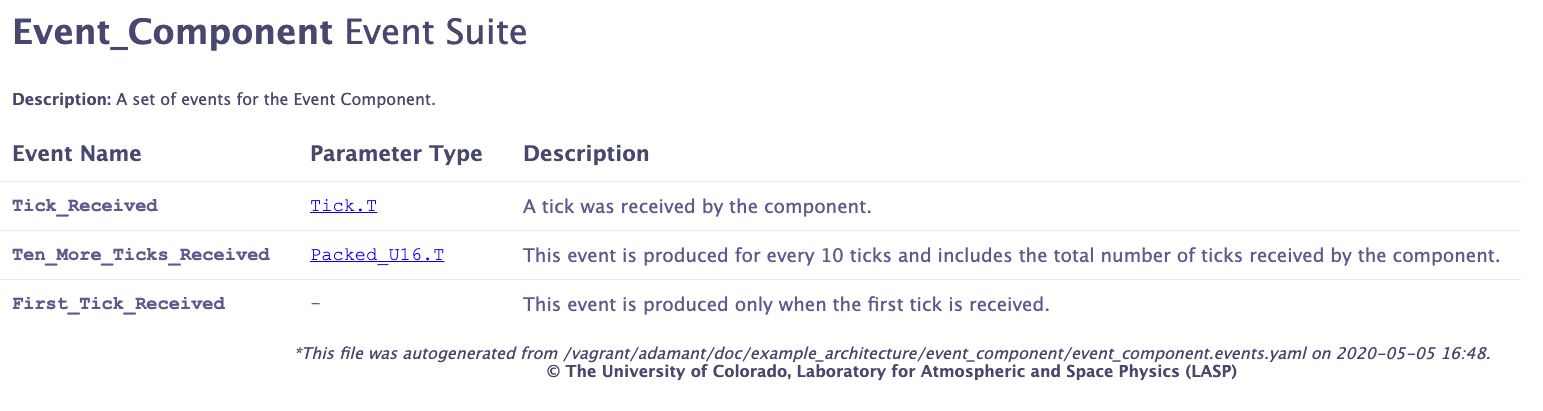
\includegraphics[width=\textwidth]{images/eventshtml.png}
\vspace{5mm} %5mm vertical space

\subsection{Component Data Products}

Data products are component \textit{IDed entities}. Please read Section \ref{Component IDed Entities} before continuing on to this section. \\

A \textit{data product} in Adamant is a small packet that contains data from onboard sensors, software state variables, etc. These are usually produced on a periodic schedule and are meant to reflect the state of the system.

\subsubsection{The Data Product Type} \label{The Data Product Type}

The data product type in Adamant is defined in \textit{src/core/types/data\_product}. A data product consists of a header followed by a byte array used to serialize the specific data, the type, associated with a data product. A data product is a \textit{variable length packed record}, see Section \ref{Variable Length Packed Records}, whose length is specified by the length field in its header. The following tables show the bit layout of a data product and its header. \\

\input{../../src/types/data_product/build/tex/data_product_header.tex}
\input{../../src/types/data_product/build/tex/data_product.tex}

As can be seen, in the header there is a 64-bit timestamp which signifies when the data product was created followed by a unique identifier for the data product. There is also a byte array where the data product's type is serialized. \\

\subsubsection{Creating a Data Product Model}

In Adamant, data products are produced by components. A component may produce many different data products. To demonstrate this we will create a component called the \textit{data\_product\_component} using the following commands:

\vspace{5mm} %5mm vertical space
\begin{minted}{text}
> mkdir data_product_component # make component directory
> cd data_product_component 
> touch .all_path              # add directory to build path
\end{minted}
\vspace{5mm} %5mm vertical space

Next we will create the component by writing the following YAML file in this directory: \\

\textit{data\_product\_component.component.yaml:}
\yamlcodef{../example_architecture/data_product_component/data_product_component.component.yaml}

which looks like this:

\begin{figure}[H]
  \includegraphics[width=0.9\textwidth,center]{../example_architecture/data_product_component/build/eps/data_product_component.eps}
\end{figure}

To configure the component with data products we use a data product model file. To create a data product model for this component, we simply need to name the data product model appropriately. Data product models will always be of the form \textit{component\_name.data\_products.yaml} where \textit{component\_name} is the component that will be producing the data products. Only a single data product model can be configured for a component, and a single data product model cannot be shared by more than one component. In this directory we create a data product model named \textit{data\_product\_component.data\_products.yaml}. The contents are shown below: \\

\textit{data\_product\_component.data\_products.yaml:}
\yamlcodef{../example_architecture/data_product_component/data_product_component.data_products.yaml}

This model defines the \textit{data product suite} for the \textit{data\_product\_component}. It declares 2 different data products that can be sent by the component. Comments are provided to explain whether or not each field is optional or required. In this case, you must supply a name for each data product and the type that will be serialized into the data product's buffer. Only a single type can be provided with a data product. However, that type can be a compound type such as an array or record. Data product types should always be \textit{packed types}, see Section \ref{Packed Types}, since their bit layout is platform independent. This allows development machines to easily decode data product values no matter what machine is running the Adamant embedded system. \\

The presence of a data product model causes the Adamant build system to produce many more build rules (some output omitted for brevity):

\vspace{5mm} %5mm vertical space
\begin{minted}{text}
> redo what 
redo  what
redo all
redo build/html/data_product_component_data_products.html
redo build/obj/Linux/data_product_component_data_products-representation.o
redo build/obj/Linux/data_product_component_data_products.o
redo build/src/data_product_component_data_products-representation.adb
redo build/src/data_product_component_data_products-representation.ads
redo build/src/data_product_component_data_products.adb
redo build/src/data_product_component_data_products.ads
\end{minted}
\vspace{5mm} %5mm vertical space

We can see two object files that can be constructed, the data product suite package, \textit{\url{build/obj/Linux/data\_product\_component\_data\_products.o}}, and the data product string representation package, \textit{\url{build/obj/Linux/data\_product\_component\_data\_products-representation.o}}, which will be discussed in Section \ref{Data Product String Representation}. To build the data product suite package autocode we can run:

\vspace{5mm} %5mm vertical space
\begin{minted}{text}
> redo build/obj/Linux/data_product_component_data_products.o
\end{minted}
\vspace{5mm} %5mm vertical space

which will construct the package \texttt{Data\_Product\_Component\_Data\_Products} in \textit{build/src/data\_product\_component\_data\_products.ads} and \textit{build/src/data\_product\_component\_data\_products.adb}. Let's look at the specification. \\

\textit{data\_product\_component\_data\_products.ads}:
\adacodef{../example_architecture/data_product_component/build/src/data_product_component_data_products.ads}

First we can see that there is a \texttt{Instance} type which is the data product suite tagged type. There is also a public \texttt{local\_Data\_Product\_Id\_Type} enumeration which declares the \textit{local IDs} for the data products. When instantiated in a component, these local IDs will be added to the component's \textit{data product ID base}. The data product ID base can be set through the public function \texttt{set\_Id\_Base} which is called during component initialization, see Section \ref{Component Set ID Bases}. Note that the ID base for the data product suite is stored in the \texttt{Instance} record in the private section in the \texttt{id\_Base} variable. Next, there is a set of two functions which return the ID for each data product in the data product suite. The returned ID will already have the ID base offset applied to the local ID. Finally, there is a set of two functions that are used to create the two data products. \\

The most commonly used functions are the data product creation functions. Each function returns a type of \texttt{Data\_Product.T} and takes a timestamp and the data product type as input. The implementation of these functions are not shown here but can be explored by the reader in \textit{data\_product\_component\_data\_products.adb}. These functions take the timestamp and data product type and serialize them into the data product header and buffer, respectively. The data product is returned with the correct ID applied. To see how these functions are used within a component continue to the next section.

\subsubsection{Using the Data Product Package}

When a data product model is found for a component, the component base package autocode is altered slightly to include a variable called \texttt{data\_products} which is an instantiation of the data product suite package instance, \texttt{Data\_Product\_Component\_Data\_Products.Instance}. The reader can verify this by building and inspecting \textit{build/src/component-data\_product\_component.ads}. This \texttt{data\_products} variable can then be used in the component implementation package to create data\_products. \\

The following is the hand-coded implementation package body for the \textit{data\_product\_component}. For directions on generating the templates for this file see Section \ref{Component Implementation Package}. \\

\textit{component-data\_product\_component-implementation.adb}:
\adacodef{../example_architecture/data_product_component/component-data_product_component-implementation.adb}

As can be seen, the component record contains the variable \texttt{Self.Count} which is sent out as a data product. Data products are constructed using the data product creation functions provided by \texttt{Self.Data\_Products}, which is an instantiation of \texttt{Data\_Product\_Component\_Data\_Products.Instance}. Data products are created and then sent out of the \texttt{Data\_Product\_T\_Send} connector.

\subsubsection{Data Product Unit Testing}

This section assumes you know how to unit test component which is described in Section \ref{Component Unit Testing}. The details of creating a unit test model, generating tester component, and implementing unit tests are not repeated here. Instead, this section will show the important differences involved when unit testing a component that has data products. \\

Below is a unit test implementation package that provides a single unit test, \texttt{Unit\_Test}, for the \textit{data\_product\_component}. \\

\textit{data\_product\_component\_tests-implementation.adb}:
\adacodef{../example_architecture/data_product_component/test/data_product_component_tests-implementation.adb}

If a component has a data product model, the autocoded tester package includes some modifications to make unit testing data products simpler. Just as with connectors, a distinct history is included for every data product defined in the component's data product model within the tester component. This history can be queried and assertions can be run against it in the same way you would a connector history. \\

As can be seen in the unit test code above, some \texttt{Tick.T}s are sent to the component which causes data products to be produced. The total number of data products produced is checked using the data product connector history. The amount and content of each individual data product received is checked by asserting against the individual data product histories provided in the tester component. \\

To run this unit test code we use:

\vspace{5mm} %5mm vertical space
\begin{minted}{text}
> redo test
\end{minted}
\vspace{5mm} %5mm vertical space

which produces the output:

\vspace{5mm} %5mm vertical space
\inputminted{text}{../example_architecture/data_product_component/test/output.txt}
\vspace{5mm} %5mm vertical space

\subsubsection{Data Product String Representation} \label{Data Product String Representation}

Similar to \textit{packed types}, Section \ref{Packed Record String Representation}, a string representation package can be produced for data products which supplies ``pretty printing" capabilities. To build this package run:

\vspace{5mm} %5mm vertical space
\begin{minted}{text}
> redo build/obj/Linux/data_product_component_data_products-representation.o
\end{minted}
\vspace{5mm} %5mm vertical space

This generates the source files \textit{build/src/data\_product\_component\_data\_products-representation.ads} and \textit{build/src/data\_product\_component\_data\_products-representation.adb}. The autocoded specification is shown below.

\adacodef{../example_architecture/data_product_component/build/src/data_product_component_data_products-representation.ads}

The \texttt{*\_Image} functions above, provided for each data product defined in the data product model, are useful for printing or logging data products during component unit test.

\subsubsection{Data Product Documentation}

Adamant provides automatic generation of documentation for any data product model. Currently two versions of documentation can be created: HTML, which is useful for presentation in meetings or for quick reference, and PDF (via \LaTeX), which is useful for formal documentation. PDF documentation for data products is created as part of component documentation and is not discussed here. See Section \ref{Component Documentation} for details. \\

To build HTML documentation run:

\vspace{5mm} %5mm vertical space
\begin{minted}{text}
> redo build/html/data_product_component_data_products.html
\end{minted}
\vspace{5mm} %5mm vertical space

which when opened with your favorite web browser looks something like this: \\

\vspace{5mm} %5mm vertical space
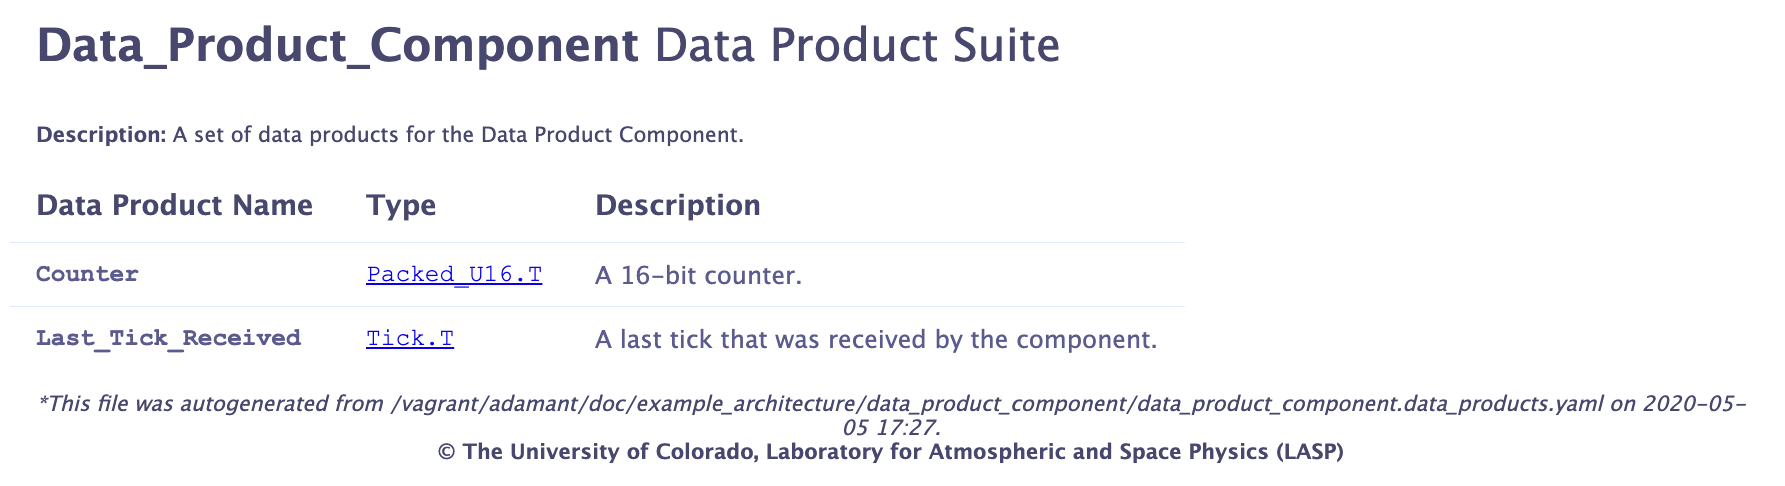
\includegraphics[width=\textwidth]{images/dataproductshtml.png}
\vspace{5mm} %5mm vertical space

\subsection{Component Data Dependencies} \label{Component Data Dependencies}

Data dependencies are component \textit{IDed entities}. Please read Section \ref{Component IDed Entities} before continuing on to this section. \\

A \textit{data dependency} in Adamant is simply a \textit{data product} produced by an external component that is needed by the component that declares the dependency. \textit{Data products} are produced by components and often stored in some central database. \textit{Data dependencies} are consumed/used/checked by components by fetching these \textit{data products} from the central store. \textit{Data dependencies} are often used by components to check the outside state of the system prior to making decisions or to perform computations based on values that are not produced inside the component. \\

Each \textit{data dependency} must declare its \textit{type} and, in the assembly, be mapped to a corresponding \textit{data product} of the same type. In this way, the producer component and consumer component of the data are decoupled, removing any compile-time dependence within the code, and type safety is enforced by the assembly model mapping.

\subsubsection{The Data Product Fetch and Return Types}

Data dependencies are designed to be fetched from a central store of data products upon request from the calling component. This is implemented by a \texttt{request} connector with the \textit{type} \texttt{Data\_Product\_Fetch.T} and \textit{return\_type} \texttt{Data\_Product\_Return.T} (found in \textit{src/core/types/data\_product}) which are shown below. \\

\input{../../src/types/data_product/build/tex/data_product_fetch.tex}
\input{../../src/types/data_product/build/tex/data_product_return.tex}

As can be seen, the \texttt{Data\_Product\_Fetch.T} type simply includes the data product identifier to fetch. The \texttt{Data\_Product\_Return.T} includes the returned data product and a status relating whether or not the fetch was successful. A data product is a compound record type that is detailed in Section \ref{The Data Product Type}. As will be seen in the next section, to use data dependencies within a component, the component must instantiate a \texttt{request} connector using these types.

\subsubsection{Creating a Data Dependency Model}

In Adamant, data dependencies are fetched by components. A component may fetch many different data dependencies of many different types, so long as those data dependencies are produced as data products of the same type by some other component in the system. To demonstrate how to use data dependencies within a component we will create a component called the \textit{data\_dependency\_component} using the following commands:

\vspace{5mm} %5mm vertical space
\begin{minted}{text}
> mkdir data_dependency_component # make component directory
> cd data_dependency_component 
> touch .all_path              # add directory to build path
\end{minted}
\vspace{5mm} %5mm vertical space

Next we will create the component by writing the following YAML file in this directory: \\

\textit{data\_dependency\_component.component.yaml:}
\yamlcodef{../example_architecture/data_dependency_component/data_dependency_component.component.yaml}

which looks like this:

\begin{figure}[H]
  \includegraphics[width=0.9\textwidth,center]{../example_architecture/data_dependency_component/build/eps/data_dependency_component.eps}
\end{figure}

Note the inclusion of the \texttt{Data\_Product\_Fetch.T}/\texttt{Data\_Product\_Return.T} \texttt{request} connector which will be used to fetch the data dependencies. \\

To configure the component with data dependencies we use a data dependency model file. To create a data dependency model for this component, we simply need to name the data dependency model appropriately. Data dependency models will always be of the form \textit{component\_name.data\_dependencies.yaml} where \textit{component\_name} is the component that will be using the data dependencies. Only a single data dependency model can be configured for a component, and a single data dependency model cannot be shared by more than one component. In this directory we create a data dependency model named \textit{data\_dependency\_component.data\_dependencies.yaml}. The contents are shown below: \\

\textit{data\_dependency\_component.data\_dependencies.yaml:}
\yamlcodef{../example_architecture/data_dependency_component/data_dependency_component.data_dependencies.yaml}

This model defines the \textit{data dependency suite} for the \textit{data\_dependency\_component}. It declares 2 different data dependencies that can be fetched by the component. Comments are provided to explain whether or not each field is optional or required. In this case, you must supply a name for each data dependency and its type. Only a single type can be provided with a data dependency. However, that type can be a compound type such as an array or record. Data dependency types should always be \textit{packed types}, see Section \ref{Packed Types}, since they must correspond to data products, which are required to be \textit{packed types}. \\

The presence of a data dependency model causes the Adamant build system to produce many more build rules (some output omitted for brevity):

\vspace{5mm} %5mm vertical space
\begin{minted}{text}
> redo what 
redo  what
redo all
redo build/html/data_dependency_component_data_dependencies.html
redo build/obj/Linux/data_dependency_component_data_dependencies.o
redo build/src/data_dependency_component_data_dependencies.adb
redo build/src/data_dependency_component_data_dependencies.ads
\end{minted}
\vspace{5mm} %5mm vertical space

We can see one object file that can be constructed, the data dependency suite package, \textit{\url{build/obj/Linux/data\_dependency\_component\_data\_dependencies.o}}. To build the data dependency suite package autocode we can run:

\vspace{5mm} %5mm vertical space
\begin{minted}{text}
> redo build/obj/Linux/data_dependency_component_data_dependencies.o
\end{minted}
\vspace{5mm} %5mm vertical space

which will construct the package \texttt{Data\_Dependency\_Component\_Data\_Dependencies} in \textit{build/src/data\_dependency\_component\_data\_dependencies.ads} and \textit{build/src/data\_dependency\_component\_data\_dependencies.adb}. Let's look at the specification. \\

\textit{data\_dependency\_component\_data\_dependencies.ads}:
\adacodef{../example_architecture/data_dependency_component/build/src/data_dependency_component_data_dependencies.ads}

Unlike for data products, packets, and events, this package is not intended to be used directly by the component implementation that it is associated with. This package is instead used within the component's base package autocode, which wraps these functions with a more friendly interface for the developer, detailed in the next section. \\

However, it is important to know what is included in this package. First, we can see that there is a \texttt{Instance} type, which is the data dependency suite tagged type. Stored in this \texttt{Instance} record is the ID to fetch for each data dependency. By default these are simply enumerated started at zero to make unit testing simpler. In a deployed assembly, however, these values are overridden to the appropriate IDs for their corresponding data products via the \texttt{Set\_Ids\_And\_Limits} procedure. This gets called as part of the assembly ided entity initialization and is discussed further in Section \ref{Component Set Data Dependency IDs}. \\

Also provided as an input parameter to the \texttt{Set\_Ids\_And\_Limits} initialization procedure are \textit{stale limits} for each data dependency. The stale limit is an Ada \texttt{Time\_Span} type which is used to determine if a fetched data dependency's timestamp is too old to be considered valid. For example, if the stale limit is set to 1 second, and the timestamp of the data dependency is more than 1 second older than the current time, the data product is considered to be stale, or too old to use. The numerical values used for the stale limits are set at the assembly modeling level, and eventually get passed to the \texttt{Set\_Ids\_And\_Limits} procedure during initialization. These stale limits are store in the \texttt{Instance} record. Note that a stale limit value of zero indicates that the data dependency can never go stale. A periodically produced data product like a temperature may reasonably go stale if it stops being produced, however some data products such as a system mode may only be produced when they are changed. Thus some data products may be considered valid, even if they are days, months, or years older than the current time. Due to this mission specific nature, stale limits must necessarily be set at the assembly modeling level. See \ref{Modeling an Assembly} for more details on how these limits are set at the assembly level. \\

For each data dependency there are two functions provided. The first retrieves the data dependency's ID, ie. \texttt{Get\_Counter\_Id}, and the other parses out the data dependency type from a generic data product, ie. \texttt{Extract\_Counter}. Again, these functions rarely need to be called directly by component implementation code, but it is good to know they exist. We will discuss how they get used in the following section.

\subsubsection{Fetching Data Dependencies}

When a data dependency model is found for a component, the component base package autocode is altered to include helper functions for fetching data dependencies. When a data dependency request is issued by the component the base package does the following:

\vspace{5mm} %5mm vertical space
\begin{spacedenumerate}
  \item The data dependency ID is retrieved using the data dependency autocoded package discussed in the previous section.
  \item The data dependency ID is passed out the \texttt{Data\_Product\_Fetch.T} connector.
  \item The data dependency is returned synchronously within a \texttt{Data\_Product\_Return.T} type that also includes the status from the request.
  \item If the status is not set to \texttt{Success}, then an \texttt{Error} or \texttt{Not\_Available} is returned to the implementation package, whichever is appropriate.
  \item If the status is set to \texttt{Success}, then the data dependency is extracted from the data product using the extraction functions discussed in the previous section.
  \item Extracting a data dependency may fail and, if so, an \texttt{Error} status is returned to the caller.
  \item The data dependency timestamp may be too old and, if so, a \texttt{Stale} status is returned to the caller.
  \item If extraction succeeds, then the extracted data dependency is returned to the caller with its timestamp and a status as to whether or not the operation failed or not.
\end{spacedenumerate}
\vspace{5mm} %5mm vertical space

The reader can verify this logic by building and inspecting \textit{build/src/component-data\_dependency\_component.ads} and \textit{build/src/component-data\_dependency\_component.adb} packages. To see the data dependency interface that can be used in the implementation package, let's look at the base package specification. \\

\textit{component-data\_dependency\_component.ads}:
\adacodef{../example_architecture/data_dependency_component/build/src/component-data_dependency_component.ads}

The bottom section of the specification is what we are most interested in. Note that for each data dependency there are two helper functions defined. The each do the same thing, except one does not pass back the data dependency timestamp to the caller. As an example, for the \texttt{Counter} data dependency we can see there is a \texttt{Get\_Counter} function. This is meant to be called directly from the implementation package to fetch data dependencies. The \texttt{Get\_Counter} function returns the counter value, its timestamp, and a status relating the success or failure of the operation. The \texttt{stale\_Reference} parameter is used to check if the data dependency is stale with respect to some time reference. Usually the current time is passed as the \texttt{stale\_Reference}. A stale return value indicates that the data product is too old to be considered valid to use within the component. The measure of ``too old" is determined by the value of \texttt{stale\_Reference}, which is the time reference (usually the current time), and \textit{stale limit}, which is defined for each data dependency at initialization (in the assembly model, as we will see in Section \ref{Modeling an Assembly}). The \textit{stale limit} is a timespan that determines how much older than \texttt{stale\_Reference} is still considered an unstale data dependency. In other words, any data dependency fetched with a timestamp that is older than \texttt{stale\_Reference} minus \textit{stale limit} is considered stale and will produce a return status of \texttt{Stale} to the caller. \\

Next, let us discuss how we can use these functions within the component implementation. The following is the hand-coded implementation package specification and body for the \textit{data\_dependency\_component}. For directions on generating the templates for these file see Section \ref{Component Implementation Package}. Looking at the specification first, we can see a few new procedures of note. \\

\textit{component-data\_dependency\_component-implementation.ads}:
\adacodef{../example_architecture/data_dependency_component/component-data_dependency_component-implementation.ads}

The data dependency primitives \texttt{Get\_Data\_Dependency} and \texttt{Invalid\_Data\_Dependency} have been included. The first is the user defined implementation for how to fetch a data dependency given a data product ID. In almost all cases this is usually just implemented via the call \texttt{Self.Data\_Product\_Fetch\_T\_Request((id => id))}, which is why it is implemented that way by default. As a general rule, the Adamant component base package does not make connector calls, and reserves that right for the implementation package only, which is why it is defined in the implementation specification, and not in the base package. If your component fetches data dependencies in a different manner, than this function can be replaced by your custom implementation. \\

The \texttt{Invalid\_Data\_Dependency} procedure is called whenever a data dependency is received that is considered invalid. In a well formed assembly, invalid data dependencies should never be encountered, as checks are performed at the modeling level to ensure that this cannot happen. Nevertheless, if one of these issues should be detected by the autocoded base package, this procedure will be called. Usually the implementation of this procedure sends out an informational event alerting of the failure. Below are the possible reasons that this procedure might be called:

\vspace{5mm} %5mm vertical space
\begin{spaceditemize}
  \item The data dependency ID requested is out of range as determined by the data product central store.
  \item The data product ID returned does not match the data dependency ID requested.
  \item The data product returned has an unexpected length that does not match the data dependency type's length.
\end{spaceditemize}
\vspace{5mm} %5mm vertical space

Since data product and data dependency IDs are assigned by the assembly model and checked for type consistency, the following errors can only result if their is a misconfigured assembly, or a bug in either the modeling autocode or the component. \\

Now let's look at the implementation package body to see how to fetch data dependencies. \\

\textit{component-data\_dependency\_component-implementation.adb}:
\adacodef{../example_architecture/data_dependency_component/component-data_dependency_component-implementation.adb}

Besides the \texttt{Invalid\_Data\_Dependency} procedure, which just prints out an error message if an invalid data dependency is received, the only subprogram included is the \texttt{Tick.T} connector handler. This would likely be tied to a rate group and get called periodically in a running assembly. The implementation of the handler does two things: 1) It grabs the \texttt{Counter} data dependency and reports its value via a print message, and 2) It grabs the \texttt{Temperature} data dependency and checks it against a static limit if it is both valid. Both data dependencies are also checked to make sure they are not stale. \\

The \texttt{Counter} data dependency and its corresponding timestamp is requested via the \texttt{Get\_Counter} function. Note that the return status of this function should be checked prior to using the returned counter value, as it may not be valid. If \texttt{Success} is returned, then the counter is valid and can be used. If \texttt{Not\_Available} is returned, then there is not corresponding data product available yet in the central store to relate the value of the counter. In this case, the returned value for \texttt{cnt} should not be used. If \texttt{Stale} is returned then the data dependency's timestamp was older than the \texttt{stale\_Reference} (the current time in this case) minus the data dependency's \textit{stale limit}. Using a data dependency that is stale can be problematic, and should be avoided. Finally, if \texttt{Error} is returned, then something unexpected happened, and you should also not use \texttt{cnt}. Note that an \texttt{Error} return value will only be returned after a call to \texttt{Invalid\_Data\_Dependency} has been made by the base package. In this way, the component developer can encapsulate all error handling for invalid data dependencies in this single subprogram. \\

The \texttt{Temperature} data dependency is requested via the \texttt{Get\_Temperature} function and is checked in a similar fashion. The next section will describe how to unit test component that uses data dependencies. \\

\subsubsection{Data Dependency Unit Testing}

This section assumes you know how to unit test component which is described in Section \ref{Component Unit Testing}. The details of creating a unit test model, generating tester component, and implementing unit tests are not repeated here. Instead, this section will show the important differences involved when unit testing a component that has data dependencies. \\

Below is a unit test implementation package that provides a single unit test, \texttt{Unit\_Test}, for the \textit{data\_dependency\_component}. \\

\textit{data\_dependency\_component\_tests-implementation.adb}:
\adacodef{../example_architecture/data_dependency_component/test/data_dependency_component_tests-implementation.adb}

If a component has a data dependency model, the autocoded tester package includes some modifications to make unit testing data products simpler. First, a variable for each data dependency is included within the tester package, ie. \texttt{Self.Tester.Counter} and \texttt{Self.Tester.Temperature}. The value of these variables is returned directly to the component when the data dependencies are requested. Note that by default, during unit testing the \textit{stale limits} of all data dependencies is initialized to 1 second. So if a data dependency is received that is older than one second when compared to the unit test time, \texttt{Self.Tester.System\_Time} then it will look stale to the component. \\

In the unit test, the first thing we do is set these variables to reasonable value. Next, we send a \texttt{Tick.T} to the component to tell it to grab these data dependencies. Next, we set the temperature to a value above the static limit and sent the \texttt{Tick.T} again. \\

The subsequent tests are used to cover the different paths a component can take when checking the data dependency statuses. In the third section we set the special \texttt{Self.Tester.Data\_Dependency\_Timestamp\_Override} variable to a non-zero timestamp. This tells the tester to send this timestamp with any requested data dependencies instead of the simulated system time, \texttt{Self.Tester.System\_Time}. In this case we also set \texttt{Self.Tester.System\_Time} such that the returned \texttt{Temperature} data dependency will be determined to be stale by the component under test. \\

The fourth section sets another special tester variable \texttt{Self.Tester.Data\_Dependency\_Return\_Id\_Override}. When non-zero, the tester component will return the value of this variable with every requested data dependency. In this way you can simulate a misconfigured system that should cause the component to receive an \texttt{Error} status. \\

In the final section we set the special tester variable \texttt{Self.Tester.Data\_Dependency\_Return\_Status\_Override} which allows us to simulate a different response than \texttt{Success} when a component requests a data dependency. In this case we set it to \texttt{Not\_Available} to see how the component responds. \\

Note that there is one additional special tester variable available (but not demonstrated) called \texttt{data\_Dependency\_Return\_Length\_Override}. When non-zero, the tester component will return the value of this variable as the data dependency length. You can use this to simulate a misconfigured system in addition to the \texttt{Self.Tester.Data\_Dependency\_Return\_Id\_Override} variable. \\

To run this unit test code we use:

\vspace{5mm} %5mm vertical space
\begin{minted}{text}
> redo test
\end{minted}
\vspace{5mm} %5mm vertical space

which produces the output:

\vspace{5mm} %5mm vertical space
\inputminted{text}{../example_architecture/data_dependency_component/test/output.txt}
\vspace{5mm} %5mm vertical space

We can see that we have exercised full coverage of all the paths that this component can execute in its implementation package.

\subsubsection{Data Dependency Documentation}

Adamant provides automatic generation of documentation for any data dependency model. Currently two versions of documentation can be created: HTML, which is useful for presentation in meetings or for quick reference, and PDF (via \LaTeX), which is useful for formal documentation. PDF documentation for data dependencies is created as part of component documentation and is not discussed here. See Section \ref{Component Documentation} for details. \\

To build HTML documentation run:

\vspace{5mm} %5mm vertical space
\begin{minted}{text}
> redo build/html/data_dependency_component_data_dependencies.html
\end{minted}
\vspace{5mm} %5mm vertical space

which when opened with your favorite web browser looks something like this: \\

\vspace{5mm} %5mm vertical space
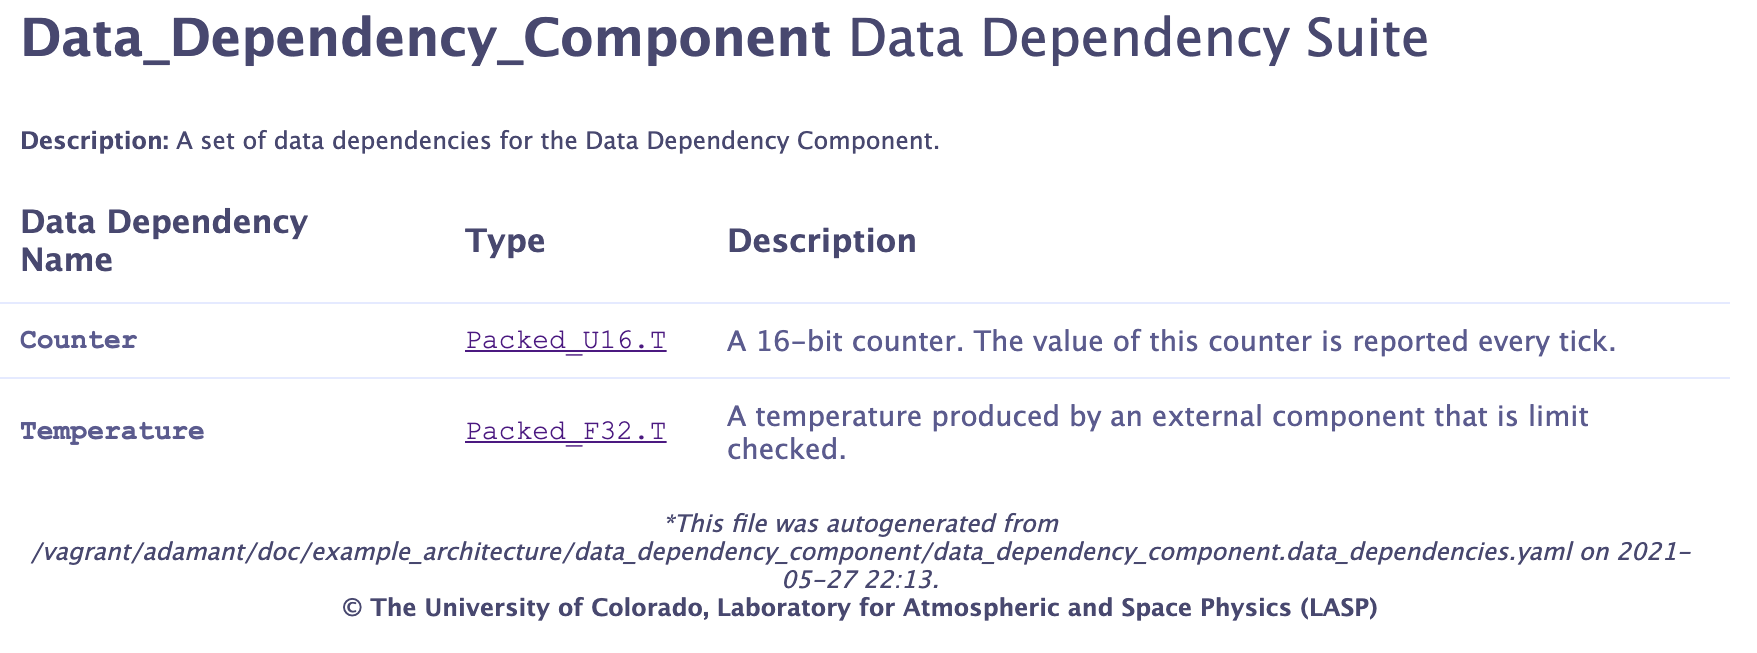
\includegraphics[width=\textwidth]{images/datadependencieshtml.png}
\vspace{5mm} %5mm vertical space

\subsection{Component Packets} \label{Component Packets}

Packets are component \textit{IDed entities}. Please read Section \ref{Component IDed Entities} before continuing on to this section. \\

\textit{Packets} are similar to \textit{data products}, but usually larger. Often, a packet contains many \textit{data products} within. \textit{Packets} are also often used for external communication.

\subsubsection{The Packet Type}

The packet type in Adamant is defined in \textit{src/core/types/packet}. A packet consists of a header followed by a byte array used to serialize the specific data, the type, associated with a packet. A packet is a \textit{variable length packed record}, see Section \ref{Variable Length Packed Records}, whose length is specified by the length field in its header. The following tables show the bit layout of a packet and its header. \\

\input{../../src/types/packet/build/tex/packet_header.tex}
\input{../../src/types/packet/build/tex/packet.tex}

As can be seen, in the header there is a 64-bit timestamp which signifies when the packet was created followed by a unique identifier for the packet. A packet also contains a \texttt{Sequence\_Count} which increments with every packet that is created. This can be used by a packet receiver to determine if any packets have been dropped or to correctly order received data. There is also a byte array where the packet's type is serialized. \\

\subsubsection{Creating a Packet Model}

In Adamant, packets are produced by components. A component may produce many different packets. To demonstrate this we will create a component called the \textit{packet\_component} using the following commands:

\vspace{5mm} %5mm vertical space
\begin{minted}{text}
> mkdir packet_component  # make component directory
> cd packet_component 
> touch .all_path         # add directory to build path
\end{minted}
\vspace{5mm} %5mm vertical space

Next we will create the component by writing the following YAML file in this directory: \\

\textit{packet\_component.component.yaml:}
\yamlcodef{../example_architecture/packet_component/packet_component.component.yaml}

which looks like this:

\begin{figure}[H]
  \includegraphics[width=0.9\textwidth,center]{../example_architecture/packet_component/build/eps/packet_component.eps}
\end{figure}

To configure the component with packets we use a packet model file. To create a packet model for this component, we simply need to name the packet model appropriately. Packet models will always be of the form \textit{component\_name.packets.yaml} where \textit{component\_name} is the component that will be producing the packets. Only a single packet model can be configured for a component, and a single packet model cannot be shared by more than one component. In this directory we create a packet model named \textit{packet\_component.packets.yaml}. The contents are shown below: \\

\textit{packet\_component.packets.yaml:}
\yamlcodef{../example_architecture/packet_component/packet_component.packets.yaml}

This model defines the \textit{packet suite} for the \textit{packet\_component}. It declares 2 different packets that can be sent by the component. Comments are provided to explain whether or not each field is optional or required. In this case, you must supply a name for each packet and the type that will be serialized into the packet's buffer. Only a single type can be provided with a packet. However, that type can be a compound type such as an array or record. Packet types should always be \textit{packed types}, see Section \ref{Packed Types}, since their bit layout is platform independent. This allows development machines to easily decode packet values no matter what machine is running the Adamant embedded system. The type for the packet is optional. If not specified, the user must fill in the packet data using a generic byte array, which will be shown in the following section. \\

Unique to packets (and faults, as we will see later), a developer may also specify the ID for each packet. If specified, the ID refers to the global ID of the packet as defined in the assembly. In this case, there is no packet \textit{id base}. This feature should only be used if you are constructing a mission-specific component, where you want to define static IDs for all the packets it creates. For reusable components, it is advised to not specify the ID for any packets, and to use the normal \texttt{Set\_Id\_Base} method for setting packet IDs, see Section \ref{Component Set ID Bases}. By not statically defining the packet IDs, the component remains reusable for future systems. \\

Note that if you define a static global ID for one packet, you MUST define the ID for every packet in the suite, as we have done here. Similarly, if you wish to not define the static IDs for the packets, you must NOT define the packet IDs for every packet in the packet suite. \\

The presence of a packet model causes the Adamant build system to produce many more build rules (some output omitted for brevity):

\vspace{5mm} %5mm vertical space
\begin{minted}{text}
> redo what 
redo  what
redo all
redo build/html/packet_component_packets.html
redo build/obj/Linux/packet_component_packets-representation.o
redo build/obj/Linux/packet_component_packets.o
redo build/src/packet_component_packets-representation.adb
redo build/src/packet_component_packets-representation.ads
redo build/src/packet_component_packets.adb
redo build/src/packet_component_packets.ads
\end{minted}
\vspace{5mm} %5mm vertical space

We can see two object files that can be constructed, the packet suite package, \textit{\url{build/obj/Linux/packet\_component\_packets.o}}, and the packet string representation package, \textit{\url{build/obj/Linux/packet\_component\_packets-representation.o}}, which will be discussed in Section \ref{Packet String Representation}. To build the packet suite package autocode we can run:

\vspace{5mm} %5mm vertical space
\begin{minted}{text}
> redo build/obj/Linux/packet_component_packets.o
\end{minted}
\vspace{5mm} %5mm vertical space

which will construct the package \texttt{Packet\_Component\_Packets} in \textit{build/src/packet\_component\_packets.ads} and \textit{build/src/packet\_component\_packets.adb}. Let's look at the specification. \\

\textit{packet\_component\_packets.ads}:
\adacodef{../example_architecture/packet_component/build/src/packet_component_packets.ads}

First, we can see that there is a \texttt{Instance} type which is the packet suite tagged type. There is also a public \texttt{local\_Packet\_Id\_Type} enumeration which declares the \textit{local IDs} for the packets. In this case, the IDs are actually the global IDs that were defined in the packet model. Notice that the \texttt{Instance} type does not have an \texttt{id\_Base} variable and there is no \texttt{set\_Id\_Base} procedure defined. The local IDs will be directly used within the packets and cannot be modified at initialization. If the IDs were omitted from the packet model, then the autocoder would generate an \texttt{id\_Base} variable and a \texttt{set\_Id\_Base} procedure and the packet IDs would be set normally at initialization, see Section \ref{Component Set ID Bases}. \\

Also take note of the two variables defined within the \texttt{Instance} record. These are used to keep track of the sequence number for each packet. These numbers are incremented and stored in the packet header every time a new packet is created, so the user does not have to worry about filling in that field. \\

Next is a set of two functions which return the ID for each packet in the packet suite. \\

Following, are the packet creation functions. The most commonly used functions are the packet creation functions. Each function returns a type of \texttt{Packet.T} and takes a timestamp and the packet type as input. The implementation of these functions are not shown here but can be explored by the reader in \textit{packet\_component\_packets.adb}. These functions take the timestamp and packet type and serialize them into the packet header and buffer, respectively. The packet is returned with the correct ID and sequence count applied. \\

The \texttt{Last\_Tick\_Received} function looks similar to the data product creation functions that we saw in the previous sections. The \texttt{Counter} function comes in three varieties, due to the fact that a packet \texttt{type} was not declared in the packet model for the \texttt{Counter} packet. The first function, \texttt{Counter}, constructs the packet using a supplied byte array. If the byte array is too large to fit in the packet then a \texttt{Failure} status is returned through the \texttt{Serialization\_Status} return type. Otherwise, the byte array is copied into the packet, the length is set appropriately, and the constructed packet is returned through the \texttt{out} parameter. The \texttt{Counter\_Truncate} function is the same as the \texttt{Counter} function, except that if the supplied byte array is too large, then any bytes larger than the packet buffer are simply discarded and a maximum sized packed is returned. Finally, the \texttt{Counter\_Empty} function returns a packet with the header set with the correct ID, sequence count, and timestamp. The packet's data is not filled in, and the user is expected to populate it manually before sending the packet out. This function should be used if filling the packet with data is more complicated than the other functions allow. \\

To see how these functions are used within a component continue to the next section.

\subsubsection{Using the Packet Package}

When a packet model is found for a component, the component base package autocode is altered slightly to include a variable called \texttt{packets} which is an instantiation of the packet suite package instance, \texttt{Packet\_Component\_Packets.Instance}. The reader can verify this by building and inspecting \textit{build/src/component-packet\_component.ads}. This \texttt{packets} variable can then be used in the component implementation package to create packets. \\

The following is the hand-coded implementation package body for the \textit{packet\_component}. For directions on generating the templates for this file see Section \ref{Component Implementation Package}. \\

\textit{component-packet\_component-implementation.adb}:
\adacodef{../example_architecture/packet_component/component-packet_component-implementation.adb}

As can be seen, the component record contains the variable \texttt{Self.Count} which is sent out as a packet. Packets are constructed using the packet creation functions provided by \texttt{Self.Packets}, which is an instantiation of \texttt{Packet\_Component\_Packets.Instance}. Packets are created and then sent out of the \texttt{packet\_T\_Send} connector. Note that since no type was provided for the \texttt{Counter} packet in the model, we have to supply our own byte array to populate the packet. In this case, they byte array is generated by serializing the \texttt{Self.Count} value using the \texttt{Packed\_U16} packed record serialization function.

\subsubsection{Packet Unit Testing}

This section assumes you know how to unit test component which is described in Section \ref{Component Unit Testing}. The details of creating a unit test model, generating tester component, and implementing unit tests are not repeated here. Instead, this section will show the important differences involved when unit testing a component that has packets. \\

Below is a unit test implementation package that provides a single unit test, \texttt{Unit\_Test}, for the \textit{packet\_component}. \\

\textit{packet\_component\_tests-implementation.adb}:
\adacodef{../example_architecture/packet_component/test/packet_component_tests-implementation.adb}

If a component has a packet model, the autocoded tester package includes some modifications to make unit testing packets simpler. Just as with connectors, a distinct history is included for every packet defined in the component's packet model within the tester component. This history can be queried and assertions can be run against it in the same way you would a connector history. \\

As can be seen in the unit test code above, some \texttt{Tick.T}s are sent to the component which causes some packets to be produced. The total number of packets produced is checked using the packet connector history. The amount and content of each individual packet received is checked by asserting against the individual packet histories provided in the tester component. Note that because the \texttt{Counter} packet does not have a defined packet type, the history simply stores the entire packet itself. In this case, we just check the first two bytes of the packet buffer to ensure that the data inside matches the values we expect. \\

To run this unit test code we use:

\vspace{5mm} %5mm vertical space
\begin{minted}{text}
> redo test
\end{minted}
\vspace{5mm} %5mm vertical space

which produces the output:

\vspace{5mm} %5mm vertical space
\inputminted{text}{../example_architecture/packet_component/test/output.txt}
\vspace{5mm} %5mm vertical space

\subsubsection{Packet String Representation} \label{Packet String Representation}

Similar to \textit{packed types}, Section \ref{Packed Record String Representation}, a string representation package can be produced for packets which supplies ``pretty printing" capabilities. To build this package run:

\vspace{5mm} %5mm vertical space
\begin{minted}{text}
> redo build/obj/Linux/packet_component_packets-representation.o
\end{minted}
\vspace{5mm} %5mm vertical space

This generates the source files \textit{build/src/packet\_component\_packets-representation.ads} and \textit{build/src/packet\_component\_packets-representation.adb}. The autocoded specification is shown below.

\adacodef{../example_architecture/packet_component/build/src/packet_component_packets-representation.ads}

The \texttt{*\_Image} functions above, provided for each packet defined in the packet model, are useful for printing or logging packets during component unit test.

\subsubsection{Packet Documentation}

Adamant provides automatic generation of documentation for any packet model. Currently two versions of documentation can be created: HTML, which is useful for presentation in meetings or for quick reference, and PDF (via \LaTeX), which is useful for formal documentation. PDF documentation for packets is created as part of component documentation and is not discussed here. See Section \ref{Component Documentation} for details. \\

To build HTML documentation run:

\vspace{5mm} %5mm vertical space
\begin{minted}{text}
> redo build/html/packet_component_packets.html
\end{minted}
\vspace{5mm} %5mm vertical space

which when opened with your favorite web browser looks something like this: \\

\vspace{5mm} %5mm vertical space
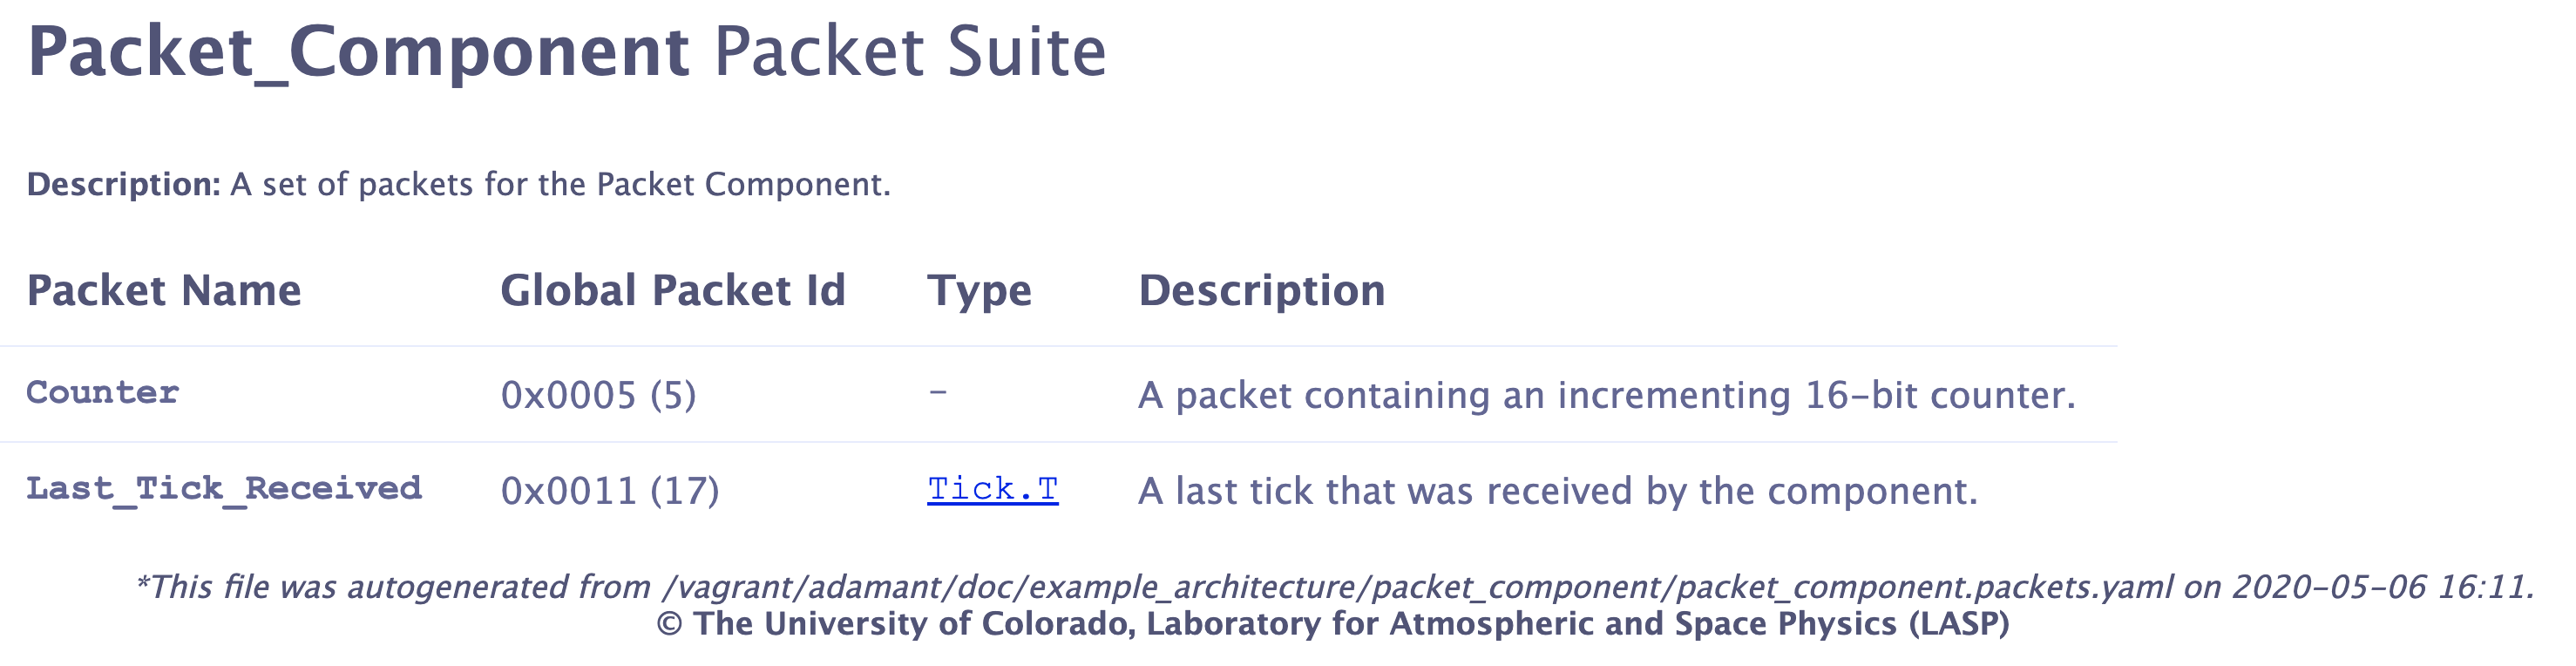
\includegraphics[width=\textwidth]{images/packetshtml.png}
\vspace{5mm} %5mm vertical space

\subsection{Component Commands} \label{Commands}

Commands are component \textit{IDed entities}. Please read Section \ref{Component IDed Entities} before continuing on to this section. \\

\textit{Commands} are packets created by an external system that are received by the embedded software and ``executed". \textit{Commands} are used to direct the software to perform certain actions at certain times.

\subsubsection{The Command Type}

The command type in Adamant is defined in \textit{src/core/types/command}. A command consists of a header followed by a byte array used to serialize the specific data, the command arguments, associated with a command. A command is a \textit{variable length packed record}, see Section \ref{Variable Length Packed Records}, whose length is specified by the length field in its header. The following tables show the bit layout of a command and its header. \\

\input{../../src/types/command/build/tex/command_header.tex}
\input{../../src/types/command/build/tex/command.tex}

As can be seen, in the header there is a unique identifier for the command, commonly referred to as the ``opcode". There is also a \texttt{Source\_Id} field which indicates which component in the system (or externally) the command originated from. Finally, there is a byte array where the command's argument is serialized. \\

\subsubsection{Creating a Command Model}

In Adamant, commands are executed by components, and in some rare cases, also produced by components. This section will discuss the first case. A component may execute many different commands. To demonstrate this we will create a component called the \textit{command\_component} using the following steps:

\vspace{5mm} %5mm vertical space
\begin{minted}{text}
> mkdir command_component  # make component directory
> cd command_component 
> touch .all_path          # add directory to build path
\end{minted}
\vspace{5mm} %5mm vertical space

Next we will create the component by writing the following YAML file in this directory: \\

\textit{command\_component.component.yaml:}
\yamlcodef{../example_architecture/command_component/command_component.component.yaml}

which looks like this:

\begin{figure}[H]
  \includegraphics[width=0.9\textwidth,center]{../example_architecture/command_component/build/eps/command_component.eps}
\end{figure}

Note that the component has two connectors. In the Adamant command system, every component has one connector to receive commands and a second connector on which to send back a \textit{command response}, which indicates whether or not the command succeeded or failed during execution. \\

To configure the component with commands we use a command model file. To create a command model for this component, we simply need to name the command model appropriately. Command models will always be of the form \textit{component\_name.commands.yaml} where \textit{component\_name} is the component that will be executing the commands. Only a single command model can be configured for a component, and a single command model cannot be shared by more than one component. In this directory we create a command model named \textit{command\_component.commands.yaml}. The contents are shown below: \\

\textit{command\_component.commands.yaml:}
\yamlcodef{../example_architecture/command_component/command_component.commands.yaml}

This model defines the \textit{command suite} for the \textit{command\_component}. It declares 2 different commands that can be sent to the component for execution. Comments are provided to explain whether or not each field is optional or required. In this case, you must supply a name for each command. Optionally you can provide an argument type that will be serialized into the command's buffer. Only a single argument type can be provided with a command. However, that type can be a compound type such as an array or record. Command types should always be \textit{packed types}, see Section \ref{Packed Types}, since their bit layout is platform independent. This allows development machines to easily construct properly formatted commands no matter what machine is running the Adamant embedded system. \\

The presence of a command model causes the Adamant build system to produce many more build rules (some output omitted for brevity):

\vspace{5mm} %5mm vertical space
\begin{minted}{text}
> redo what 
redo  what
redo all
redo build/html/command_component_commands.html
redo build/obj/Linux/command_component_commands.o
redo build/src/command_component_commands.adb
redo build/src/command_component_commands.ads
\end{minted}
\vspace{5mm} %5mm vertical space

We can see one object file that can be constructed, the command suite package, \textit{\url{build/obj/Linux/command\_component\_commands.o}}. To build the command suite package autocode we can run:

\vspace{5mm} %5mm vertical space
\begin{minted}{text}
> redo build/obj/Linux/command_component_commands.o
\end{minted}
\vspace{5mm} %5mm vertical space

which will construct the package \texttt{Command\_Component\_Commands} in \textit{build/src/command\_component\_commands.ads} and \textit{build/src/command\_component\_commands.adb}. Let's look at the specification. \\

\textit{command\_component\_commands.ads}:
\adacodef{../example_architecture/command_component/build/src/command_component_commands.ads}

Unlike for data products, packets, and events, this package is not intended to be used by the component that it is associated with. This package is used to \textit{create} commands, not \textit{execute} them, and thus is most commonly used to generate commands while unit testing the component. The commands are executed within the component itself using special autocode within the component base package, see the following section. In rare cases, an external component may use this package to create and send commands to the destination component. This pattern is commonly used for a fault response component in spacecraft flight software. Let's explore the package's contents, remembering that it will most likely be utilized by a tester component during unit test. \\

First, we can see that there is a \texttt{Instance} type, which is the command suite tagged type. There is also a public \texttt{local\_command\_Id\_Type} enumeration which declares the \textit{local IDs} for the commands. When instantiated in a component, these local IDs will be added to the component's \textit{command ID base}. The command ID base can be set through the public function \texttt{set\_Id\_Base} which is called during component initialization, see Section \ref{Component Set ID Bases}. Note that the ID base for the command suite is stored in the \texttt{Instance} record in the private section in the \texttt{id\_Base} variable. \\

Also stored in the \texttt{Instance} record is a \texttt{source\_Id} variable. This variable can be set or retrieved through the \texttt{set\_Source\_Id} and \texttt{get\_Source\_Id} subprograms. The \texttt{Source\_Id} gets populated in the command header and signifies where the command is originating from. This value is generally not used by the component executing command, but is used by the Adamant standard command routing and command response forwarding system provided by the Command Router component, see \textit{src/components/command\_router}. \\

Next, there is a set of two functions which return the ID for each command in the command suite. The returned ID will already have the ID base offset applied to the local ID. Finally, there is a set of two functions that are used to create the two commands. \\

The most commonly used functions are the command creation functions. Each function returns a type of \texttt{Command.T} and takes the command argument (if there is one) as input. The implementation of these functions are not shown here but can be explored by the reader in \textit{command\_component\_commands.adb}. These functions take the command argument type and serialize it into the command buffer. The command is returned with the correct ID and source ID applied. To see how these functions are used within a unit test see Section \ref{Command Unit Testing}.

\subsubsection{Implementing Command Handlers}

When a command model is found for a component, the component base package autocode is altered to include command handling logic. When a command is received by a component the component base package does the following:

\vspace{5mm} %5mm vertical space
\begin{spacedenumerate}
  \item The command ID is checked for validity. If it is out of range an \texttt{Id\_Error} return status is set.
  \item The command length is checked for validity. If it does not match the expected length a \texttt{Length\_Error} return status is set.
  \item The command argument is checked for validity by making sure it is within the Ada range(s) defined for the argument type. If it is not valid, then a \texttt{Validation\_Error} return status is set.
  \item If all the previous checks pass, the command is passed to the implementation package command handler for execution, otherwise proceed to the last step.
  \item The command handler executes and either sets the command return status to \texttt{Success} or \texttt{Failure}.
  \item A command response is constructed using the return status and sent out of the component.
\end{spacedenumerate}
\vspace{5mm} %5mm vertical space

The reader can verify this logic by building and inspecting \textit{build/src/component-command\_component.ads} and \textit{build/src/component-command\_component.adb}. \\

Also defined in the base package is an abstract subprogram for each command that must be executed. These subprograms ensure that the command handlers are implemented within the implementation package, otherwise a compilation error will result. \\

The developer must implement the abstract command handler functions for each command defined in the base package. The following is the hand-coded implementation package body for the \textit{command\_component} with the command handlers implemented. For directions on generating the templates for this file see Section \ref{Component Implementation Package}. \\

\textit{component-command\_component-implementation.adb}:
\adacodef{../example_architecture/command_component/component-command_component-implementation.adb}

The first thing to notice is the implementation of the \texttt{Command\_T\_Recv\_Sync} connector handler. This code is completely generated by the template autocoder, and rarely needs to be modified by the developer. It first calls \texttt{execute\_Command} which calls an autocoded function in the base package that performs the procedure described above, validating and executing the command. Returned from this call is the command status, which is copied into a command response record and sent out of the component through a call to \texttt{Command\_Response\_T\_Send} connector. Note that the call to \texttt{execute\_Command} is going to, in turn, call the command handlers that are implemented just below the \texttt{Command\_T\_Recv\_Sync} procedure. \\

The two command handler functions are named after the commands that they service. The \texttt{Hello\_World} command simply prints out the famous text and then returns a \texttt{Success} status. The \texttt{Was\_Five\_Sent} handler is a bit more complicated. It checks the command argument to see if it equals 5. If so, then a \texttt{Success} status is returned, otherwise a \texttt{Failure} status is returned. \\

Note, all command handler functions return a type of \texttt{Command\_Execution\_Status.E}, which is an enumeration with only two states, \texttt{Success} and \texttt{Failure}. One of the two must be returned by the developer. The base package autocode will copy the return value into the command response message that gets forwarded out after command execution. The command response type itself is described in the following section. \\

Finally, there is a \texttt{Invalid\_Command} procedure defined. This procedure must be implemented anytime a component includes a command model. The procedure gets called by the autocoded base package if the command is not valid, ie. it does not have a valid ID, length, or command arguments. Usually this function sends out an event alerting the operator of the system that their command was invalid. In this case we just print some text to standard out. \\

\subsubsection{The Command Response Type}

The command response type in Adamant is defined in \textit{src/core/types/command}. Adamant requires a command response be sent out after any command is executed. The type itself is shown below. \\

\input{../../src/types/command/build/tex/command_response.tex}

The record contains \texttt{Source\_Id} and \texttt{Command\_Id} which are copied from the command itself. The \texttt{Registration\_Id} is used for command routing within Adamant and is not discussed here. See the Command Router component for more details, \textit{src/components/command\_router}. The most important part of the response is the \texttt{Status} field which relates if the command was successfully executed or not. The possible status enumeration literals and their numerical representations are shown. As a developer, you are only responsible for returning a command's status as \texttt{Success} or \texttt{Failure} via a return value in the command's handler function. All other status values are returned, when necessary, by the autocode within the component base package.

\subsubsection{Command Unit Testing} \label{Command Unit Testing}

This section assumes you know how to unit test component which is described in Section \ref{Component Unit Testing}. The details of creating a unit test model, generating tester component, and implementing unit tests are not repeated here. Instead, this section will show the important differences involved when unit testing a component that has commands. \\

Below is a unit test implementation package that provides a single unit test, \texttt{Unit\_Test}, for the \textit{command\_component}. \\

\textit{command\_component\_tests-implementation.adb}:
\adacodef{../example_architecture/command_component/test/command_component_tests-implementation.adb}

If a component has a command model, the autocoded tester package includes some modifications to make unit testing commands simpler. Included in the tester base package \texttt{Instance} record is a variable called \texttt{Commands} which is of the type \texttt{Command\_Component\_Commands.Instance}. As can be seen in the unit test code above, the \texttt{Self.Tester.Commands} variable is used to construct commands that are then sent to the component on the \texttt{Command.T} send connector. After the command is sent, the unit test makes sure that a command response is returned by the component into the command response connector history. The command responses are checked for \texttt{Success} or \texttt{Failure} where appropriate. \\

To run this unit test code we use:

\vspace{5mm} %5mm vertical space
\begin{minted}{text}
> redo test
\end{minted}
\vspace{5mm} %5mm vertical space

which produces the output:

\vspace{5mm} %5mm vertical space
\inputminted{text}{../example_architecture/command_component/test/output.txt}
\vspace{5mm} %5mm vertical space

\subsubsection{Command Documentation}

Adamant provides automatic generation of documentation for any command model. Currently two versions of documentation can be created: HTML, which is useful for presentation in meetings or for quick reference, and PDF (via \LaTeX), which is useful for formal documentation. PDF documentation for commands is created as part of component documentation and is not discussed here. See Section \ref{Component Documentation} for details. \\

To build HTML documentation run:

\vspace{5mm} %5mm vertical space
\begin{minted}{text}
> redo build/html/command_component_commands.html
\end{minted}
\vspace{5mm} %5mm vertical space

which when opened with your favorite web browser looks something like this: \\

\vspace{5mm} %5mm vertical space
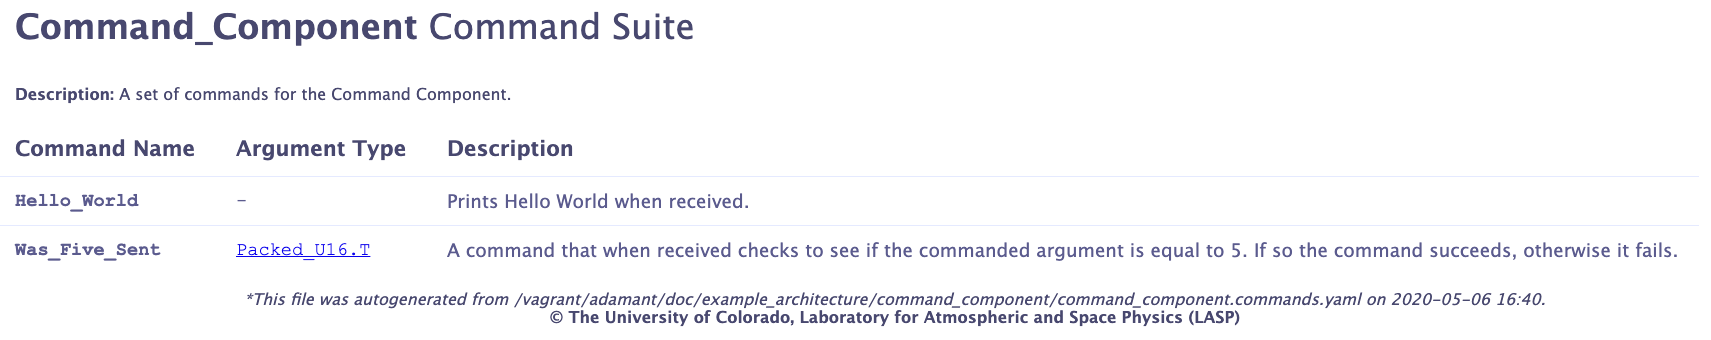
\includegraphics[width=\textwidth]{images/commandshtml.png}
\vspace{5mm} %5mm vertical space

\subsection{Component Parameters} \label{Component Parameters}

Parameters are component \textit{IDed entities}. Please read Section \ref{Component IDed Entities} before continuing on to this section. \\

\textit{Parameters} are values that are used to configure a component. Parameters are often stored in a single location on the embedded system, and can be changed by an external system to reconfigure it. Changes to these parameters are then ``pushed" to components to change their behavior.

\subsubsection{The Parameter Type}

The parameter type in Adamant is defined in \textit{src/core/types/parameter}. A parameter consists of a header followed by a byte array used to serialize the specific data, the type, associated with a parameter. A parameter is a \textit{variable length packed record}, see Section \ref{Variable Length Packed Records}, whose length is specified by the length field in its header. The following tables show the bit layout of a parameter and its header. \\

\input{../../src/types/parameter/build/tex/parameter_header.tex}
\input{../../src/types/parameter/build/tex/parameter.tex}

As can be seen, in the header there is a unique identifier for the parameter. There is also a byte array where the parameter's serialized type is stored. \\

\subsubsection{The Parameter Update Type} \label{The Parameter Update Type}

The parameter type itself is does not contain enough information to allow effective updating of parameters through connectors in the system, so a \texttt{Parameter\_Update} type has been created for this purpose. The type is located in \textit{src/core/types/parameter/parameter\_update.record.yaml} and has the following layout. \\

\input{../../src/types/parameter/build/tex/parameter_update.tex}

As can be seen the \texttt{Parameter\_Update} type contains an additional \texttt{Operation} field which states whether or not to \textit{Stage}, \textit{Update}, or \textit{Fetch} the parameter, concepts that will be discussed in the following sections. It also contains a \texttt{Status} field which returns the status of the operation as executed by the receiving component. The possible status enumeration literals and their numerical representations are shown. As a developer, you never need to set the parameter update status, as this is completely handled by the base package autocode.  More details on updating parameters are discussed in the following sections.

\subsubsection{Creating a Parameter Model}

In Adamant, parameters are used by components to configure their behavior. A component may contain many different parameters. To demonstrate this we will create a component called the \textit{parameter\_component} using the following steps:

\vspace{5mm} %5mm vertical space
\begin{minted}{text}
> mkdir parameter_component  # make component directory
> cd parameter_component 
> touch .all_path            # add directory to build path
\end{minted}
\vspace{5mm} %5mm vertical space

Next we will create the component by writing the following YAML file in this directory: \\

\textit{parameter\_component.component.yaml:}
\yamlcodef{../example_architecture/parameter_component/parameter_component.component.yaml}

which looks like this:

\begin{figure}[H]
  \includegraphics[width=0.9\textwidth,center]{../example_architecture/parameter_component/build/eps/parameter_component.eps}
\end{figure}

Note that the component has two connectors. The first is the \texttt{Tick.T} connector which drives the execution of the component. The second is the \texttt{Parameter\_Update.T} modify connector which allows the component's parameters to be updated during execution. The \texttt{Parameter\_Update.T} modify connector will return a status that relates whether or not the parameter was successfully updated or not. \\

To configure the component with parameters we use a parameter model file. To create a parameter model for this component, we simply need to name the parameter model appropriately. Parameter models will always be of the form \textit{component\_name.parameters.yaml} where \textit{component\_name} is the component that will be executing the parameters. Only a single parameter model can be configured for a component, and a single parameter model cannot be shared by more than one component. In this directory we create a parameter model named \textit{parameter\_component.parameters.yaml}. The contents are shown below: \\

\textit{parameter\_component.parameters.yaml:}
\yamlcodef{../example_architecture/parameter_component/parameter_component.parameters.yaml}

This model defines the \textit{parameter suite} for the \textit{parameter\_component}. It declares 2 different parameters that are used to configure the component. Comments are provided to explain whether or not each field is optional or required. In this case, you must supply a name for each parameter. You must also provide the type for each parameter. Only a single type can be used to described a parameter. However, that type can be a compound type such as an array or record. Parameter types should always be \textit{packed types}, see Section \ref{Packed Types}, since their bit layout is platform independent. This allows development machines to easily construct properly formatted parameters no matter what machine is running the Adamant embedded system. A default value must also be provided for each parameter. The parameter within the component will be initialized to this value on startup and will only be overridden when a new value is set from a parameter managing component externally. \\

The presence of a parameter model causes the Adamant build system to produce many more build rules (some output omitted for brevity):

\vspace{5mm} %5mm vertical space
\begin{minted}{text}
> redo what 
redo  what
redo all
redo build/html/parameter_component_parameters.html
redo build/obj/Linux/parameter_component_parameters.o
redo build/src/parameter_component_parameters.adb
redo build/src/parameter_component_parameters.ads
\end{minted}
\vspace{5mm} %5mm vertical space

We can see one object file that can be constructed, the parameter suite package, \textit{\url{build/obj/Linux/parameter\_component\_parameters.o}}. To build the parameter suite package autocode we can run:

\vspace{5mm} %5mm vertical space
\begin{minted}{text}
> redo build/obj/Linux/parameter_component_parameters.o
\end{minted}
\vspace{5mm} %5mm vertical space

which will construct the package \texttt{Parameter\_Component\_Parameters} in \textit{build/src/parameter\_component\_parameters.ads} and \textit{build/src/parameter\_component\_parameters.adb}. Let's look at the specification. \\

\textit{parameter\_component\_parameters.ads}:
\adacodef{../example_architecture/parameter_component/build/src/parameter_component_parameters.ads}

Unlike for data products, packets, and events, this package is not intended to be used by the component that it is associated with. This package is used to \textit{create} parameters, not \textit{use} them, and thus is most commonly used to generate parameters while unit testing the component. The parameters are stored and updated within the component itself using special autocode within the component base package, see the following section. Let's explore the package's contents, remembering that it will most likely be utilized by a tester component during unit test. \\

First, we can see that there is a \texttt{Instance} type, which is the parameter suite tagged type. There is also a public \texttt{local\_Parameter\_Id\_Type} enumeration which declares the \textit{local IDs} for the parameters. When instantiated in a component, these local IDs will be added to the component's \textit{parameter ID base}. The parameter ID base can be set through the public function \texttt{set\_Id\_Base} which is called during component initialization, see Section \ref{Component Set ID Bases}. Note that the ID base for the parameter suite is stored in the \texttt{Instance} record in the private section in the \texttt{id\_Base} variable. \\

Next, there is a set of two functions which return the ID for each parameter in the parameter suite. The returned ID will already have the ID base offset applied to the local ID. Finally, there is a set of two functions that are used to create the two parameters. \\

The most commonly used functions are the parameter creation functions. Each function returns a type of \texttt{Parameter.T} and takes the parameter type as input. The implementation of these functions are not shown here but can be explored by the reader in \textit{parameter\_component\_parameters.adb}. These functions take the parameter type and serialize it into the parameter buffer. The parameter is returned with the correct ID applied. To see how these functions are used within a unit test see Section \ref{Parameter Unit Testing}.

\subsubsection{Updating and Using Parameters}

When a parameter model is found for a component, the component base package \texttt{Instance} record is altered to contain those parameter variables. For our \textit{parameter\_component}, two variables are added to the base package \texttt{Instance} record: \texttt{Start\_Count} and \texttt{Hello\_World\_Value}. These variables can be accessed just like any other component variable, ie. via \texttt{Self.Start\_Count} and \texttt{Self.Hello\_World\_Value}. The only difference is that these variables can be updated or fetched by a call to the component's \texttt{Parameter\_Update.T} modify connector. \\

Note that if the type of the parameter is a \textit{packed type}, then the \texttt{U} version of the type is used within the component base package \texttt{Instance} record for the best performance. Since the \texttt{U} type uses the machine native representation of the variable, it often provides faster access than the packed type. \\

The two variables added to the base class are called the \textit{working} parameters, because these are the values that are directly used by the component during execution. In addition to the \textit{working} parameters, there is also a set of protected \textit{staged} parameters that assist in the updating of the \textit{working} parameter values in a thread-safe and performant manner. The \textit{staged} parameters act as a temporary holding place for updated parameter values, and are copied to the \textit{working} values atomically, when the component deems it is safe to do so. The details of this process are discussed in the remainder of this section. \\

To handle parameter updating, the component base package autocode is altered to include additional logic to process the \texttt{Parameter\_Update.T} data. As seen in Section \ref{The Parameter Update Type}, the \texttt{Parameter\_Update.T} type contains a field \texttt{Operation} which determines the type of processing that the component base package needs to perform. The processing performed for the different \texttt{Operation}s are as follows:

\vspace{5mm} %5mm vertical space
\begin{spaceditemize}
  \item \textbf{\texttt{Stage}} - The incoming parameter value is checked for validity in ID, length, and range and then stored within a temporary \textit{staged} variable within the component.
  \item \textbf{\texttt{Update}} - This operation indicates that all new parameter values have been \textit{staged} and are ready to be copied to the \textit{working} variables within the component.
  \item \textbf{\texttt{Fetch}} - The \textit{staged} value of the parameter with the indicated ID is returned to the invoker.
\end{spaceditemize}
\vspace{5mm} %5mm vertical space

The \texttt{Fetch} operation is the most straightforward. The current \textit{staged} value of the parameter is simply returned to the caller. The \texttt{Stage} and \texttt{Update} operations are a bit more sophisticated and are described further. \\

When a parameter \texttt{Stage} operation is received by a component, the component base package does the following:

\vspace{5mm} %5mm vertical space
\begin{spacedenumerate}
  \item The parameter ID is checked for validity. If it is out of range an \texttt{Id\_Error} return status is set.
  \item The parameter length is checked for validity. If it does not match the expected length a \texttt{Length\_Error} return status is set.
  \item The parameter type is checked for validity by making sure it is within the Ada range(s) defined for that type. If it is not valid, then a \texttt{Validation\_Error} return status is set.
  \item If all the previous checks pass, the parameter is ``staged", ie. stored in a \textit{staged} variable.
  \item The set parameter status is returned to the parameter update invoker.
\end{spacedenumerate}
\vspace{5mm} %5mm vertical space

The reader can verify this logic by building and inspecting \textit{build/src/component-parameter\_component.ads} and \textit{build/src/component-parameter\_component.adb}. \\

Note that after validation, a parameters is not immediately copied over to the component \texttt{Instance} variables holding the parameters. Instead the parameters are ``staged", ie. copied to a temporary staging variable. This is done for a few reasons:

\vspace{5mm} %5mm vertical space
\begin{spacedenumerate}
  \item We do not want to update the component's parameters at the same time the component is executing. This could cause unintended behavior. Instead, we want to let the component implementation itself determine when the best time to update parameters is.
  \item We want to make sure that updating all of the component's parameters is atomic, that is, all parameters are updated together. We don't want to get into a state where one parameter is updated, but another is still not updated. This could also cause unintended behavior.
\end{spacedenumerate}
\vspace{5mm} %5mm vertical space

To circumvent these issues, parameters are staged. A component is alerted that all new values for parameters have been staged when the \texttt{Update} operation is received on the \texttt{Parameter\_Update.T} connector. Once alerted, the component is able to atomically update its local parameter variables stored in \texttt{Instance} by making a call to the autocoded base package procedure \texttt{Update\_Parameters}. This procedure will copy all the parameters from the staging area to their working local copy in \texttt{Instance}. The call to this function will only execute this logic after all parameters for the component have been staged, ie. once the \texttt{Update} operation has been received, making sure the parameters are updated atomically. \\

The following is the hand-coded implementation package body for the \textit{parameter\_component} which demonstrates how to properly use parameters within a component. For directions on generating the templates for this file see Section \ref{Component Implementation Package}. \\

\textit{component-parameter\_component-implementation.adb}:
\adacodef{../example_architecture/parameter_component/component-parameter_component-implementation.adb}

The first thing to notice is the implementation of the \texttt{Parameter\_Update\_T\_Modify} connector handler. This code is completely generated by the template autocoder, and rarely needs to be modified by the developer. It calls \texttt{Process\_Parameter\_Update} which is an autocoded procedure in the base package that performs the procedure described above, processing the parameter update based on the specified \texttt{Operation}. Returned from this call is the parameter status which is returned to the connector caller (via \texttt{in out} procedure parameter). \\

The next procedure, \texttt{Tick\_T\_Recv\_Sync} represents the main execution of the component. In this procedure, we first call \texttt{Self.Update\_Parameters}, which is implemented in the component base package. As described earlier, if all the parameters for the component have been staged through calls to \texttt{Parameter\_Update\_T\_Modify} from an external component (as indicated by the \texttt{Update} operation), then this function will atomically copy those staged parameters to their working copies in the component \texttt{Instance} record. If an \texttt{Update} has not yet been received, then the call to \texttt{Update\_Parameters} does nothing and returns instantly. \\

Next, we access one of the component's parameters, \texttt{Self.Hello\_World\_Value.Value}, and compare it against our \texttt{Self.Count} variable, which is incremented every time a \texttt{Tick.T} is received. If \texttt{Self.Count} is equal to our parameter value, then the famous string is printed. \\

The standard practice when using parameters within components is to call \texttt{Self.Update\_Parameters} at the beginning of execution to make sure that all parameters are up to date before continuing on. Once the parameters are atomically updated, they can be used freely. \\

The next procedure that is defined is \texttt{Update\_Parameters\_Action}. This procedure gets called any time the parameters have been successfully updated via a call to \texttt{Self.Update\_Parameters}. Note that it is not called if not all the parameters have been staged yet, ie. an \texttt{Update} operation has not yet been received. By default, the implementation of this procedure is \texttt{null}, and it rarely needs to actually be implemented by the developer. The purpose of the procedure is to allow the developer to implement an action that runs whenever the parameters have been updated. This is often used to keep hardware state in sync with software parameters. For instance, one can use this procedure to write parameter values to hardware registers. In this way, you can always ensure that if the software parameter values get updated, so do the analogous hardware registers. \\

In this case, we use the \texttt{Update\_Parameters\_Action} procedure to update our local variable \texttt{Self.Count} with the parameter value \texttt{Self.Start\_Count.Value} anytime the parameters are updated. In this way, the parameters can be used to set \texttt{Self.Count} to any value during execution.

\subsubsection{Parameter Unit Testing} \label{Parameter Unit Testing}

This section assumes you know how to unit test component which is described in Section \ref{Component Unit Testing}. The details of creating a unit test model, generating tester component, and implementing unit tests are not repeated here. Instead, this section will show the important differences involved when unit testing a component that has parameters. \\

Below is a unit test implementation package that provides a single unit test, \texttt{Unit\_Test}, for the \textit{parameter\_component}. \\

\textit{parameter\_component\_tests-implementation.adb}:
\adacodef{../example_architecture/parameter_component/test/parameter_component_tests-implementation.adb}

If a component has a parameter model, the autocoded tester package includes some modifications to make unit testing parameters simpler. Included in the tester base package \texttt{Instance} record is a variable called \texttt{Parameters} which is of the type \texttt{Parameter\_Component\_Parameters.Instance}. As can be seen in the unit test code above, the \texttt{Self.Tester.Parameters} variable is used to construct parameters. \\

In addition to \texttt{Self.Tester.Parameters}, three helper functions are autocoded into the tester component implementation package to aid in the unit testing of parameters. They are described below:

\vspace{5mm} %5mm vertical space
\begin{spaceditemize}
  \item \textbf{\texttt{Stage\_Parameter}} - Stage a parameter within the component under test.
  \item \textbf{\texttt{Update\_Parameters}} - Send the \texttt{Update} operation to the component under test, allowing it to copy parameter values form \textit{staged} to \textit{active} upon a call to \texttt{Update\_Parameters}.
  \item \textbf{\texttt{Fetch\_Parameter}} - Get the value of a parameter (the \textit{staged} copy) within the component under test.
\end{spaceditemize}
\vspace{5mm} %5mm vertical space

If you look at the autocoded tester implementation package body (not shown here for brevity), you can see that the implementation of these helper functions simply calls the tester component's \texttt{Parameter\_Update.T} provide connector with the appropriate \texttt{Operation} set, and then returns the resulting status to the caller. Using these helper functions keeps unit test code that deals with parameters small and concise. \\

The unit test above begins by staging the component's two parameters, and subsequently fetching them to ensure that the stage worked correctly. This is achieved through calls to \texttt{Stage\_Parameter} and \texttt{Fetch\_Parameter}. For each, the status is checked to ensure that \texttt{Success} is returned. \\

After the parameters are staged, the special procedure \texttt{Self.Tester.Update\_Parameters} is called. This special parameter sends the \texttt{Update} operation to the component, signaling that the component's \textit{working} parameters can now be atomically updated by copying from the \textit{staged} via the \texttt{Update\_Parameters} procedure within the component. \\

Finally, we can verify the parameters were successfully updated by the unit test code by running it:

\vspace{5mm} %5mm vertical space
\begin{minted}{text}
> redo test
\end{minted}
\vspace{5mm} %5mm vertical space

which produces the output:

\vspace{5mm} %5mm vertical space
\inputminted{text}{../example_architecture/parameter_component/test/output.txt}
\vspace{5mm} %5mm vertical space

\subsubsection{Parameter Documentation}

Adamant provides automatic generation of documentation for any parameter model. Currently two versions of documentation can be created: HTML, which is useful for presentation in meetings or for quick reference, and PDF (via \LaTeX), which is useful for formal documentation. PDF documentation for parameters is created as part of component documentation and is not discussed here. See Section \ref{Component Documentation} for details. \\

To build HTML documentation run:

\vspace{5mm} %5mm vertical space
\begin{minted}{text}
> redo build/html/parameter_component_parameters.html
\end{minted}
\vspace{5mm} %5mm vertical space

which when opened with your favorite web browser looks something like this: \\

\vspace{5mm} %5mm vertical space
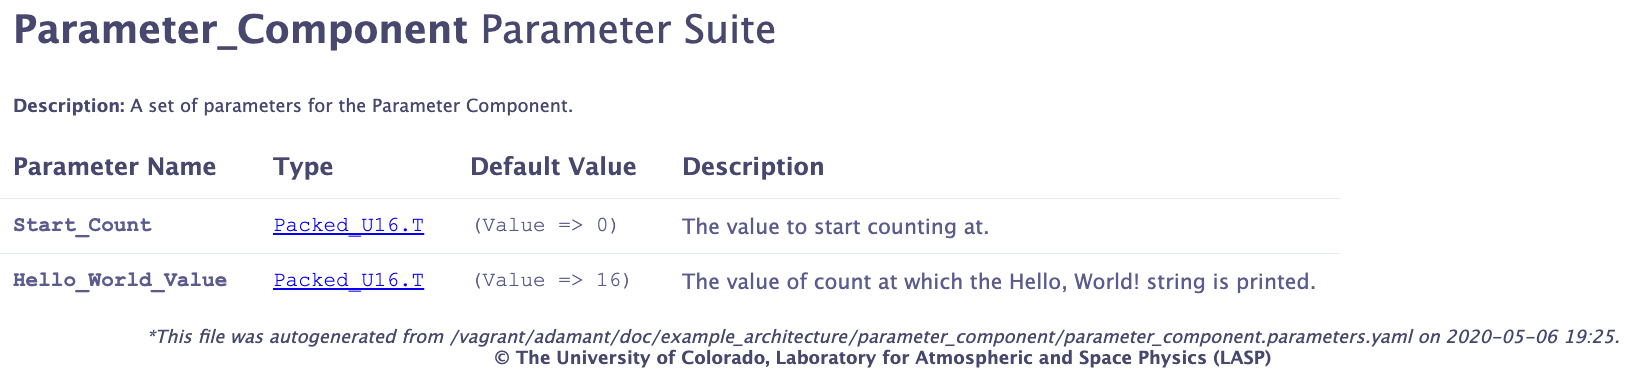
\includegraphics[width=\textwidth]{images/parametershtml.png}
\vspace{5mm} %5mm vertical space

\subsection{Component Faults}

Faults are component \textit{IDed entities}. Please read Section \ref{Component IDed Entities} before continuing on to this section. \\

A \textit{fault} in Adamant is a small asynchronously created packet that signifies that some off-nominal behavior or error condition has been encountered. Faults are usually produced in response to limit checking of telemetry, monitoring of loss on a communication channel, or due to some other anomalous condition. As a result, they are usually produced rarely and sporadically.

\subsubsection{The Fault Type}

The fault type in Adamant is defined in \textit{src/core/types/fault}. A fault consists of a header followed by a byte array used to serialize the specific data, parameters, associated with the fault. A fault is a \textit{variable length packed record}, see Section \ref{Variable Length Packed Records}, whose length is specified by the length field in its header. The following tables show the bit layout of a fault and its header. \\

\input{../../src/types/fault/build/tex/fault_header.tex}
\input{../../src/types/fault/build/tex/fault.tex}

As can be seen, in the fault header there is a 64-bit timestamp which signifies when the fault was encountered followed by a unique identifier for the fault. There is also a byte array where the fault's parameters are serialized. \\

\subsubsection{Creating a Fault Model}

In Adamant, faults are produced by components. A component may produce many different faults. To demonstrate this we will create a component called the \textit{fault\_component} using the following commands:

\vspace{5mm} %5mm vertical space
\begin{minted}{text}
> mkdir fault_component # make component directory
> cd fault_component 
> touch .all_path       # add directory to build path
\end{minted}
\vspace{5mm} %5mm vertical space

Next we will create the component by writing the following YAML file in this directory: \\

\textit{fault\_component.component.yaml:}
\yamlcodef{../example_architecture/fault_component/fault_component.component.yaml}

which looks like this:

\begin{figure}[H]
  \includegraphics[width=0.9\textwidth,center]{../example_architecture/fault_component/build/eps/fault_component.eps}
\end{figure}

To configure the component with faults we use a fault model file. To create a fault model for this component, we simply need to name the fault model appropriately. Fault models will always be of the form \textit{component\_name.faults.yaml} where \textit{component\_name} is the component that will be producing the faults. Only a single fault model can be configured for a component, and a single fault model cannot be shared by more than one component. In this directory we create a fault model named \textit{fault\_component.faults.yaml}. The contents are shown below: \\

\textit{fault\_component.faults.yaml:}
\yamlcodef{../example_architecture/fault_component/fault_component.faults.yaml}

This model defines the \textit{fault suite} for the \textit{fault\_component}. It declares 2 different faults that can be sent by the component. Comments are provided to explain whether or not each field is optional or required. In this case, you must supply a name for each fault, and optionally a parameter that will be serialized with the fault. Only a single parameter type can be provided with a fault. However, that parameter can be a compound type such as an array or record. Parameters should always be \textit{packed types}, see Section \ref{Packed Types}, since their bit layout is platform independent. This allows development machines to easily decode fault parameters no matter what machine is running the Adamant embedded system. \\

Similar to packets, a developer may also specify the ID for each fault. If specified, the ID refers to the global ID of the fault as defined in the assembly. In this case, there is no fault \textit{id base}. This feature should only be used if you are constructing a mission-specific component, where you want to define static IDs for all the faults it creates. For reusable components, it is advised to not specify the ID for any faults, and to use the normal \texttt{Set\_Id\_Base} method for setting fault IDs, see Section \ref{Component Set ID Bases}. By not statically defining the fault IDs, the component remains reusable for future systems. \\

Note that if you define a static global ID for one fault, you MUST define the ID for every fault in the suite. Similarly, if you wish to not define the static IDs for the faults, you must NOT define the fault IDs for every fault in the fault suite. \\

The presence of a fault model causes the Adamant build system to produce many more build rules (some output omitted for brevity):

\vspace{5mm} %5mm vertical space
\begin{minted}{text}
> redo what 
redo  what
redo all
redo build/html/fault_component_faults.html
redo build/obj/Linux/fault_component_faults.o
redo build/src/fault_component_faults.adb
redo build/src/fault_component_faults.ads
\end{minted}
\vspace{5mm} %5mm vertical space

We can see one object files that can be constructed, the fault suite package, \textit{\url{build/obj/Linux/fault\_component\_faults.o}}. To build the fault suite package autocode we can run:

\vspace{5mm} %5mm vertical space
\begin{minted}{text}
> redo build/obj/Linux/fault_component_faults.o
\end{minted}
\vspace{5mm} %5mm vertical space

which will construct the package \texttt{Fault\_Component\_Faults} in \textit{build/src/fault\_component\_faults.ads} and \textit{build/src/fault\_component\_faults.adb}. Let's look at the specification. \\

\textit{fault\_component\_faults.ads}:
\adacodef{../example_architecture/fault_component/build/src/fault_component_faults.ads}

First we can see that there is a \texttt{Instance} type which is the fault suite tagged type. There is also a public \texttt{local\_Fault\_Id\_Type} enumeration which declares the \textit{local IDs} for the faults. When instantiated in a component, these local IDs will be added to the component's \textit{fault ID base}. The fault ID base can be set through the public function \texttt{set\_Id\_Base} which is called during component initialization, see Section \ref{Component Set ID Bases}. Note that the ID base for the fault suite is stored in the \texttt{Instance} record in the private section in the \texttt{id\_Base} variable. Next, there is a set of 3 functions which return the ID for each fault in the fault suite. The returned ID will already have the ID base offset applied to the local ID. Finally, there is a set of three functions that are used to create the three faults. \\

The most commonly used functions are the fault creation functions. Each function returns a type of \texttt{Fault.T} and takes a timestamp and the fault parameter type as input. The implementation of these functions are not shown here but can be explored by the reader in \textit{fault\_component\_faults.adb}. These functions take the timestamp and fault parameter and serialize them into the fault header and buffer, respectively. The fault is returned with the correct ID applied. To see how these functions are used within a component continue to the next section.

\subsubsection{Using the Fault Package}

When a fault model is found for a component, the component base package autocode is altered slightly to include a variable called \texttt{faults} which is an instantiation of the fault suite package instance, \texttt{Fault\_Component\_Faults.Instance}. The reader can verify this by building and inspecting \textit{build/src/component-fault\_component.ads}. This \texttt{faults} variable can then be used in the component implementation package to create faults. \\

The following is the hand-coded implementation package body for the \textit{fault\_component}. For directions on generating the templates for this file see Section \ref{Component Implementation Package}. \\

\textit{component-fault\_component-implementation.adb}:
\adacodef{../example_architecture/fault_component/component-fault_component-implementation.adb}

As can be seen, the component record contains the variable \texttt{Self.Last\_Received\_Seconds} in which it saves off the last received \texttt{Seconds} value from the system time contained within the received \texttt{Tick.T}. The component does various error checking on this received time to determine if it is valid or not. The two error cases it looks for are a zero time (meaning time has reset) and a discontinuous time. If either of these conditions are encountered then the component will produce and send out a fault. Faults are constructed using the fault creation functions provided by \texttt{Self.Faults}, which is an instantiation of \texttt{Fault\_Component\_Faults.Instance}. Faults are created and then sent out of the \texttt{Fault\_T\_Send} connector.

\subsubsection{Fault Unit Testing}

This section assumes you know how to unit test component which is described in Section \ref{Component Unit Testing}. The details of creating a unit test model, generating tester component, and implementing unit tests are not repeated here. Instead, this section will show the important differences involved when unit testing a component that has faults. \\

Below is a unit test implementation package that provides a single unit test, \texttt{Unit\_Test}, for the \textit{fault\_component}. \\

\textit{fault\_component\_tests-implementation.adb}:
\adacodef{../example_architecture/fault_component/test/fault_component_tests-implementation.adb}

If a component has a fault model, the autocoded tester package includes some modifications to make unit testing faults simpler. Just as with connectors, a distinct history is included for every fault defined in the component's fault model within the tester component. This history can be queried and assertions can be run against it in the same way you would a connector history. \\

As can be seen in the unit test code above, some \texttt{Tick.T}s are sent to the component. The component is checking the \texttt{Seconds} value of the \texttt{Tick.T} timestamp for validity. For certain sequences of \texttt{Seconds} the unit test makes sure that the correct fault is produced. The total number of faults produced is checked using the fault connector history. The amount and content of each individual fault received is checked by asserting against the individual fault histories provided in the tester component. \\

To run this unit test code we use:

\vspace{5mm} %5mm vertical space
\begin{minted}{text}
> redo test
\end{minted}
\vspace{5mm} %5mm vertical space

which produces the output:

\vspace{5mm} %5mm vertical space
\inputminted{text}{../example_architecture/event_component/test/output.txt}
\vspace{5mm} %5mm vertical space

\subsubsection{Fault Documentation}

Adamant provides automatic generation of documentation for any fault model. Currently two versions of documentation can be created: HTML, which is useful for presentation in meetings or for quick reference, and PDF (via \LaTeX), which is useful for formal documentation. PDF documentation for faults is created as part of component documentation and is not discussed here. See Section \ref{Component Documentation} for details. \\

To build HTML documentation run:

\vspace{5mm} %5mm vertical space
\begin{minted}{text}
> redo build/html/fault_component_faults.html
\end{minted}
\vspace{5mm} %5mm vertical space

which when opened with your favorite web browser looks something like this: \\

\vspace{5mm} %5mm vertical space
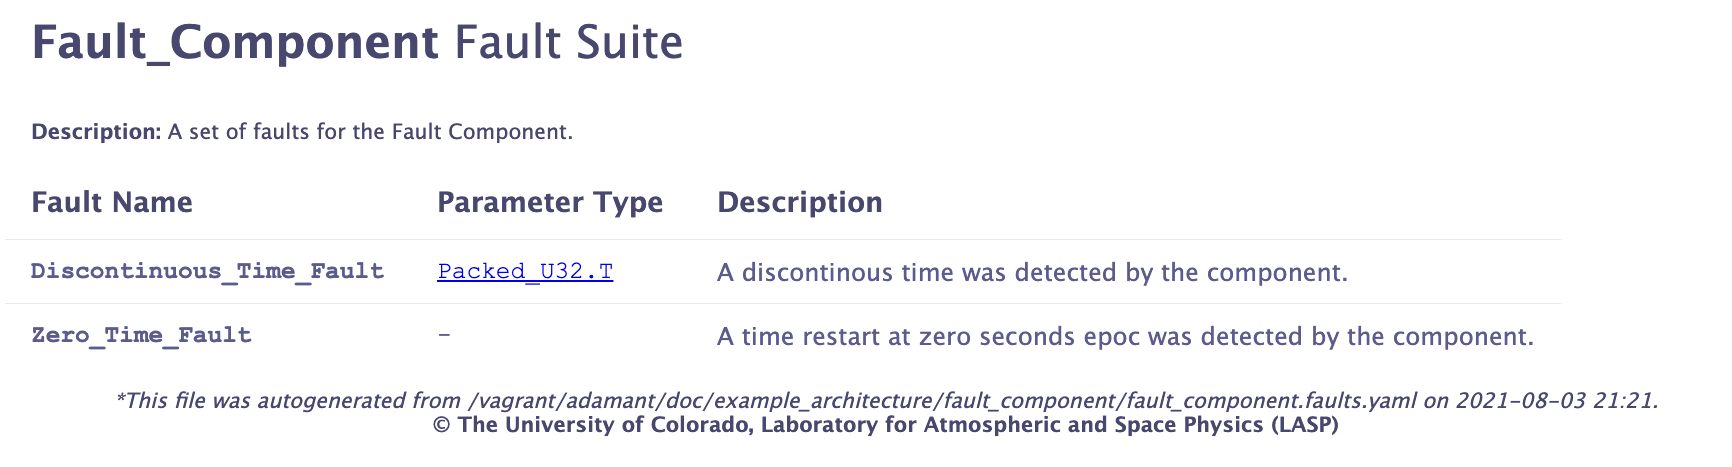
\includegraphics[width=\textwidth]{images/faultshtml.png}
\vspace{5mm} %5mm vertical space

\subsection{Component Documentation} \label{Component Documentation}

One of the benefits of the extensive modeling required by Adamant is that rich, informative documentation can be generated with little extra effort. This documentation is beneficial at all stages of the development process, from working out the details of the design, to reviewing the implementation. \\

It is advisable to generate component documentation as soon as a solid component model has been developed for a component. In this way, the document can be used to explain the design to other engineers and gain feedback before the implementation has even begun. During the development process, the design document should periodically be regenerated to reflect any changes. Finally, when the component is complete, the design document should be reviewed to ensure that it contains all the information necessary for another engineer to use or make changes to the component. Sometimes this requires adding custom sections to the design document that the document autocoder would not be able to create on its own. \\

This section walks through how to generate documentation for components and points to good examples of component documentation that exists in the Adamant repository.

\subsubsection{Component Requirements}

One of the most important aspects to designing good software is to understand what the software needs to do. These features are often captured in written ``requirements" which often stem from customer needs, design principles, or environmental constraints. When a good set of requirements has been distilled for a software component, the engineer can ensure that their design decisions are in line with what the software needs to accomplish. Finally, during test, requirements can be verified with the actual executing system to prove that the software does indeed adhere to functionality it is required to provide. \\

Currently in Adamant, requirements can be placed into a requirements model and included in the component design document. This is the currently supported functionality, but plans exist in the future to have a richer requirement feature set that includes tying requirements to the unit tests that fulfill them. \\

To specify requirements for a component we use a requirements model file. To create a requirements model for the \texttt{example\_component} presented in previous sections, we simply need to name the model appropriately. Requirement models will always be of the form \textit{component\_name.requirements.yaml} where \textit{component\_name} is the component that will be fulfilling the requirements. Only a single requirements model can be configured for a component, and a single requirements model cannot be shared by more than one component. In the \textit{example\_component} directory we create a requirements model named \textit{example\_component.requirements.yaml}. The contents are shown below: \\

\textit{example\_component.requirements.yaml:}
\yamlcodef{../example_architecture/example_component/example_component.requirements.yaml}

This model defines the \textit{requirement suite} for the \textit{example\_component}. It declares 3 different requirements that are used to constrain the design of the component. Comments are provided to explain whether or not each field is optional or required. In this case, you must supply the \texttt{text} field for each requirement that usually contains a ``shall" statement. Optionally, you may provide a \texttt{description} that elaborates or provides rational for the requirement text. \\

Requirement models in Adamant do not have a direct effect on the component's code. Currently, they can be used to produce three outputs: CSV output, HTML documentation, and PDF documentation. PDF documentation for requirements is created as part of component documentation and is discussed in the next section. \\

To build HTML documentation run:

\vspace{5mm} %5mm vertical space
\begin{minted}{text}
> redo build/html/example_component_requirements.html
\end{minted}
\vspace{5mm} %5mm vertical space

which when opened with your favorite web browser looks something like this: \\

\vspace{5mm} %5mm vertical space
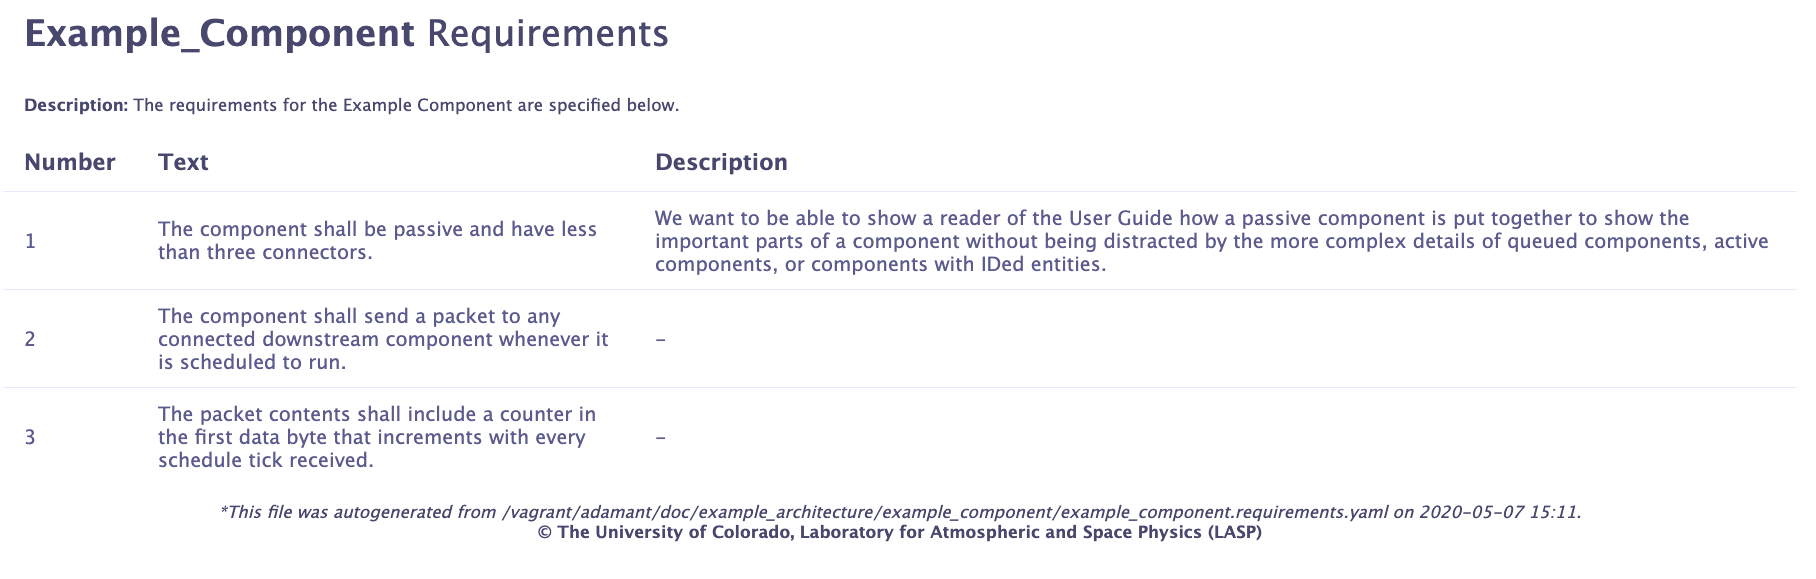
\includegraphics[width=\textwidth]{images/requirementshtml.png}
\vspace{5mm} %5mm vertical space

CSV output can be produced by running:

\vspace{5mm} %5mm vertical space
\begin{minted}{text}
> redo build/html/example_component_requirements.csv
\end{minted}
\vspace{5mm} %5mm vertical space

The CSV feature is currently incomplete and will need to be refined if it is going to be used heavily.

\subsubsection{Component Design Document} \label{Component Design Document}

One of the benefits of the extensive modeling required by Adamant is that rich, informative documentation can be generated with little extra effort. To generate documentation for a component, a component model must first exist. This section demonstrates how to generate (and modify) documentation for the \textit{example\_component} that has been discussed in previous sections. \\

Component documentation must be generated and stored in a subdirectory \textit{doc/} of the component's main directory. In fact, Adamant only produces rules to build component documentation within a \textit{doc/} directory. This convention makes it easy to locate the documentation for any component in the repository. \\

To create documentation for the \textit{example\_component} we first create the doc directory:

\vspace{5mm} %5mm vertical space
\begin{minted}{text}
> mkdir doc  # make doc/ directory under example_component/
> cd doc
\end{minted}
\vspace{5mm} %5mm vertical space

After we are inside the new \textit{doc/} directory we can view the build rules that are available.

\vspace{5mm} %5mm vertical space
\begin{minted}{text}
> redo what
redo  what
redo all
redo clean
redo clean_all
redo templates
redo publish
redo targets
redo prove
redo analyze
redo style
redo pretty
redo test_all
redo coverage_all
redo build/pdf/example_component_commands.pdf
redo build/pdf/example_component_connectors.pdf
redo build/pdf/example_component_data_products.pdf
redo build/pdf/example_component_description.pdf
redo build/pdf/example_component_enums.pdf
redo build/pdf/example_component_events.pdf
redo build/pdf/example_component_init.pdf
redo build/pdf/example_component_interrupts.pdf
redo build/pdf/example_component_packets.pdf
redo build/pdf/example_component_preamble.pdf
redo build/pdf/example_component_requirements.pdf
redo build/pdf/example_component_stats.pdf
redo build/pdf/example_component_types.pdf
redo build/pdf/example_component_unit_test.pdf
redo build/template/example_component.tex
redo build/tex/example_component_commands.tex
redo build/tex/example_component_connectors.tex
redo build/tex/example_component_data_products.tex
redo build/tex/example_component_description.tex
redo build/tex/example_component_enums.tex
redo build/tex/example_component_events.tex
redo build/tex/example_component_init.tex
redo build/tex/example_component_interrupts.tex
redo build/tex/example_component_packets.tex
redo build/tex/example_component_preamble.tex
redo build/tex/example_component_requirements.tex
redo build/tex/example_component_stats.tex
redo build/tex/example_component_types.tex
redo build/tex/example_component_unit_test.tex
\end{minted}
\vspace{5mm} %5mm vertical space

As can be seen, there are many different \textit{.tex} files that can be created, each that can be used to produce a small PDF stub of that piece of documentation. Most importantly there is a rule to build the documentation template, which is the master \LaTeX{} file for the component documentation. To build and use the template we run:

\vspace{5mm} %5mm vertical space
\begin{minted}{text}
> redo build/template/example_component.tex
> cp build/template/* .  # copy the template file into doc/
\end{minted}
\vspace{5mm} %5mm vertical space

This template provides an excellent start to our component documentation and often provides sufficient detail to be used without modification. However, like all template files in Adamant, this is meant to be modified, if necessary, to add additional hand-written documentation. Let's take a look at the autogenerated \textit{example\_component.tex} file. \\

\textit{example\_component.tex:}
\latexcodef{../example_architecture/example_component/doc/example_component.tex}

As can be seen, this file defines the sections of the component documentation and imports most of the text from external autogenerated \textit{.tex} files. Feel free to modify this file to add extra sections to the component documentation. \\

To generate a PDF from this file run:

\vspace{5mm} %5mm vertical space
\begin{minted}{text}
> redo build/pdf/example_component.pdf
\end{minted}
\vspace{5mm} %5mm vertical space

By default, PDF files are generated in the \textit{build/pdf/} directory. This allows the developer to review the output documentation before ``publishing" it, ie. saving it in the repository. Once the documentation looks good, you can publish it manually by copying it into the \textit{doc/} directory:

\vspace{5mm} %5mm vertical space
\begin{minted}{text}
> cp build/pdf/example_component.pdf .
\end{minted}
\vspace{5mm} %5mm vertical space

or alternatively you can run the special Adamant command:

\vspace{5mm} %5mm vertical space
\begin{minted}{text}
> redo publish
\end{minted}
\vspace{5mm} %5mm vertical space

which will build the documentation and perform the copy for you. \\

The produced documentation is not shown here for brevity. Below is a list of component documentation that can be found in the Adamant repository, each which demonstrates different implementation:

\vspace{5mm} %5mm vertical space
\begin{spaceditemize}
  \item \href{https://github.com/lasp/adamant/blob/main/doc/example_architecture/example_component/doc/example_component.pdf}{\textcolor{blue}{Example Component Design Document}} - The design document for the \textit{example\_component} that was generated in this section.
  \item \href{https://github.com/lasp/adamant/blob/main/src/components/command_router/doc/command_router.pdf?at=refs%2Fheads%2Fdev}{\textcolor{blue}{Command Router Design Document}} - Demonstrates how to add a ``context" diagram to the component documentation.
  \item \href{https://github.com/lasp/adamant/blob/main/src/components/ccsds/ccsds_router/doc/ccsds_router.pdf?at=refs%2Fheads%2Fdev}{\textcolor{blue}{CCSDS Router Design Document}} - Demonstrates how to add many ``context" diagrams to the component documentation to demonstrate different use cases for the component.
\end{spaceditemize}
\vspace{5mm} %5mm vertical space

\subsection{Component Metrics}

It is often valuable to keep track of certain code metrics such as the number of lines of code, packages, files, etc. for each component and component unit test. Adamant provides the ability to generate metrics for any executable, file, or object in the system. Steps to produce different metrics Adamant are discussed in Section \ref{Code Metrics}. The same example there can be applied to component packages and unit tests.

\subsection{Advanced Component Topics}

This section presents component design topics that are for more experienced Adamant users. Many of these features are not as commonly employed as the features described in previous sections. Examples may not be as in depth and may require more exploratory work by the reader. Components within the Adamant repository that demonstrate the features presented will be referenced to aid in understanding.

\subsubsection{Generic Components}

Adamant provides a feature that allows for a component to operate on one or more generic parameters. This uses the underlying Ada feature for \href{https://learn.adacore.com/courses/intro-to-ada/chapters/generics.html}{\textcolor{blue}{generic packages}}. The advantage of defining a component with generic parameters is that these parameters can be used as connector types, allowing the component to operate on data in a generic manner. The actual type that the component operates on is not determined until the generic component is instantiated in an assembly. If components can be generic, they are much more likely to be reusable. \\

Two good example components that use this feature in Adamant are the the \textit{logger} component, which logs data of a generic type to an in-memory circular buffer, \textit{src/components/loggers/logger}, and the \textit{splitter} component, which can split any \textit{send} connector into an array of outputs, \textit{src/components/splitter}. The splitter component is simple and demonstrates a minimal usage of the generic feature, so it is ideal to use as an example for this section of the document. \\

Let's begin by taking a look at the \textit{splitter} component model: \\

\textit{splitter.component.yaml:} 
\adacodef{../../src/components/splitter/splitter.component.yaml}

As can be seen, this component uses the YAML tag \texttt{generic} to define the component's generic types. An optional \texttt{description} is provided followed by a list of generic parameters. Each parameter must include a parameter \texttt{name} and optionally a \texttt{description}. \\

Each parameter can also specify two other tags that are not specified for the \textit{splitter} component, \texttt{formal\_type} and \texttt{optional}. If not specified, the \texttt{formal\_type} for the generic is assumed to be \texttt{Type T is private;}. This formal generic type has specific semantic meaning in Ada. For a list of the different formal types available in Ada see the table found in the \href{https://en.wikibooks.org/wiki/Ada_Programming/Generics#Generic_formal_types}{\textcolor{blue}{Ada Wiki}}. As can be seen from the link, the default \texttt{formal\_type} defines a generic parameter that can be any nonlimited definite type. To override this conservative generic formal type, you can specify the \texttt{formal\_type} field manually. See the \textit{logger} component for an example of manually defining a \texttt{formal\_type}. \\

If the \texttt{formal\_type} field includes a default value, you can inform the Adamant modeling system of this by setting the \texttt{optional} field to \texttt{True}. This will enable a user to instantiate the component without defining a concrete type for the generic parameter, using the provided default instead. \\

For the \textit{splitter} the name of the generic type is \texttt{T}. As you can see, the type \texttt{T} is then used for all of the \textit{splitter}'s connectors, making them of generic type. \\

If you build the component base package specification for the splitter component via:

\vspace{5mm} %5mm vertical space
\begin{minted}{text}
> redo build/src/component-splitter.ads
\end{minted}
\vspace{5mm} %5mm vertical space

you will see that the package is \texttt{generic} and contains the generic parameter \texttt{T}. The package is not shown here for brevity. \\

The generic type \texttt{T} is then used in the implementation package of the component. Below is the implementation body which shows the behavior of the \textit{splitter} component. \\

\textit{component-splitter-implementation.adb:} 
\adacodef{../../src/components/splitter/component-splitter-implementation.adb}

As can be seen, the component takes in a variable of type \texttt{T} and then forwards this out to all of its arrayed connectors. \\

Instantiation of a generic component is done in the assembly model. Below is an example instantiation of the \textit{splitter} component, using \texttt{Event.T} as the generic type. 

\vspace{5mm} %5mm vertical space
\begin{yamlcode}
components:
  - type: Splitter
    description: This component splits the event stream, sending events to 3 different outputs.
    generic_types:
      - "T => Event.T"
    init_base:
      - "T_Send_Count => 3"
  ... 
connections: 
  ...
  etc.
\end{yamlcode}
\vspace{5mm} %5mm vertical space

The new tag here is \texttt{generic\_types}, which contains a list of the generic parameter names and the types to instantiate them with.  Similar to the \texttt{init\_base} tag, all \texttt{generic\_types} must be listed as id-value pairs of the form ``\texttt{generic\_Parameter\_Name => Type}". What we have done here is turned our generic \textit{splitter} into a splitter specialized for splitting events. We can easily define a few more splitters in our assembly model for any other type we wish to split. This is the power of generic components. \\

Note that special care needs to be taken when defining a generic connector type that is of kind \textit{recv\_async}. This implies that the generic type will get serialized onto the component's internal queue. Usually in Adamant, if an \textit{recv\_async} connector is called, the type gets serialized onto the component's internal queue. If the type is a packed record of variable length, then only the bytes used in the type (usually specified by a length field in a header) will be serialized onto the queue. The same behavior is not implemented by default when using a generic type on a \textit{recv\_async} connector. By default, the maximum size of the generic type will always get serialized onto the queue. The reason for this is that the component has no way of determining the serialized length of the type, unless you explicitly provide a way. \\

For example, if a component with a generic \textit{recv\_async} connector is instantiated with the type \texttt{Command.T}, then every time a command is received by the component, the maximum size of the \texttt{Command.T} type is serialized onto the queue. To get around this behavior and allow the intelligent serialization of variable length types you MUST include an additional formal parameter in your \texttt{generic} definition in the component model named \texttt{Serialized\_Length}, which provides a function that returns the serialized length of the packed record. The definition should look like the example shown below:

\vspace{5mm} %5mm vertical space
\begin{yamlcode}
...
generic:
  description: An example showing how to define a generic type that can be variable length.
  parameters:
    - name: T
      description: The generic type of data passed to this components recv_async connector.
    - name: Serialized_Length
      description: A method that returns the serialized length of an item of type T. This is useful for serializing variable length packed types onto the queue.
      formal_type: "with function Serialized_Length(src : in T; num_Bytes_Serialized : out Natural) return Serializer_Types.Serialization_Status;"
...
etc.
\end{yamlcode}
\vspace{5mm} %5mm vertical space

When the Adamant system sees a \texttt{Serialized\_Length} function provided in the generic formal parameter list, it will automatically include the autocoded logic to intelligently serialized variable length types onto the component's internal queue. Note that all packed records defined in Adamant, whether they are variable length or not, include a \texttt{Serialized\_Length} function which fits the definition shown above. Thus this generic formal definition can be used to instantiate the component with static sized or variable length packed records alike. The underlying autocoded base package will handle both cases correctly. \\

For an example of this pattern see the \textit{Limiter} component found in \textit{src/components/generics/limiter}. The component contains unit tests that exercise the component's asynchronous connector instantiated with both a statically sized and variable length packed record.

\subsubsection{Component Interrupt Handling} \label{Component Interrupt Handling}

Adamant provides modeling support for any component that directly handles interrupts. Interrupt specific parameters such as the interrupt priority and ID are often set via the \textit{discriminant} in Ada. Indeed, you could simply use the \textit{discrimininant} tag in your component model to pass in this interrupt data, see Section \ref{Component Instantiation} but then the Adamant modeling system would not know about the interrupt. By providing a way to specify interrupts directly within a component model we are able to more readily produce documentation and other useful autocode associated with all the interrupts in the system. So if you need to handle and interrupt in your component, using the feature presented in this section is highly recommended. \\


Most interrupt handling in Adamant can be achieved by using the components found in \textit{src/components/interrupt\_handlers}. Sometimes you need to handle interrupts in a particular way that these components cannot accommodate, and thus you need to define an interrupt handling component from scratch. In this case, using the Adamant interrupt handling components will serve as good examples. In fact, we will use the Adamant \textit{interrupt\_servicer} component to demonstrate the interrupt feature in this section. \\

Let's take a look at the interrupt servicer component model which can be found in \textit{src/components/interrupt\_handlers/interrupt\_servicer/}: \\

\textit{interrupt\_servicer.component.yaml:} 
\adacodef{../../src/components/interrupt_servicer/interrupt_servicer.component.yaml}

This is a complex model that demonstrates many of the advanced features of component modeling. We can see there is a \texttt{generic} instantiation, the details of which are presented in the previous section. There is also a \texttt{discriminant} defined, details found in Section \ref{Component Instantiation}. The new tag we can see in this model is the \texttt{interrupts} tag. \\

The \texttt{interrupts} tag takes a list of interrupts that the component handles. Each interrupt is provided a \texttt{name} and an optional \texttt{description}. That is it. \\

The purpose of this tag is twofold 1) to provide the Adamant modeling system with information about all interrupts in the system for autocoding and documentation generation purposes, and 2) to allow the component's code generator to automatically insert interrupt related parameters into the component's \textit{discriminant}. We will demonstrate the second purpose by taking a look at the \textit{interrupt\_servicer}'s implementation specification: \\

\textit{component-interrupt\_servicer-implementation.ads:} 
\adacodef{../../src/components/interrupt_servicer/component-interrupt_servicer-implementation.ads}

As can be seen in the component \texttt{Instance} definition, the discriminant not only consists of the \texttt{discriminant} parameter defined in the model, \texttt{custom\_Interrupt\_Procedure}, it also has two additional parameters, \texttt{interrupt\_Id} and \texttt{interrupt\_Priority}. The second two parameters are inserted automatically due to the \texttt{interrupt} definition in the component model. We can see that these two parameters are used to instantiate a \texttt{Task\_Signal} object in the component record, whose definition can be found in the Adamant core interrupt handlers package, \textit{src/core/interrupt\_handlers}. You should consider using, or adding to, this package if you are defining a custom interrupt handling component in your system. \\

Instantiating a component with interrupts in the assembly model is no different than instantiating any other component with \texttt{discriminant} parameters defined. An example is shown below.

\vspace{5mm} %5mm vertical space
\begin{yamlcode}
components:
  - type: Interrupt_Servicer
    description: This component handles and interrupt and passes it along to the assembly.
    priority: 1
    stack_size: 2000
    secondary_stack_size: 10000
    generic_types:
      - "Interrupt_Data_Type => Tick.T"
      - "Set_Interrupt_Data_Time => Tick_Interrupt_Handler.Set_Tick_Time"
    discriminant:
      - "interrupt_Priority => System.Interrupt_Priority'Last"
      - "interrupt_Id => Ada.Interrupts.Names.SIGUSR1"
      - "custom_Interrupt_Procedure => Tick_Interrupt_Handler.Handler'Access"
  ... 
connections: 
  ...
  etc.
\end{yamlcode}
\vspace{5mm} %5mm vertical space

As can be seen, three parameters are passed into the discriminant, two of which are the interrupt specific parameters.

\subsubsection{Component Subtasks}
 
An \textit{active} component only has a single task associated with it. There are times when it makes sense to have two tasks contained inside a single component. Usually this is necessary when you need two threads of execution to handle a single piece of shared data or hardware, such as a socket. In many cases, the desired behavior can be achieved using two \textit{active} components that work in concert through protected objects. However, there are times when the cleaner design is simply to have a single component with 2 or more tasks. \\

To accomplish this, Adamant includes a component model feature to instantiate one or more \textit{subtask}s within the component. A subtask is the same as the component's \textit{active} task (if it has one), except that the behavior of the subtask must always be completely specified by the developer. \\

A good example of defining a subtask is the \textit{ccsds\_socket\_interface} component, found in \textit{src/component/ccsds\_socket\_interface/}. This component uses two tasks to manage a single socket interface. The main \textit{active} component task is responsible for waiting on the component's queue for data to send out of the socket. When data is received, it is forwarded out the socket using the \textit{active} task. A subtask is instantiated to listen on the socket for incoming data. When incoming data is received on the \textit{listener} task, it is then forwarded out to the rest of the system through a connector. By instantiating a subtask, we are able to accomplish reading and writing on a shared socket within a single component. \\

Defining a subtask must be done in the component model. Below is the component model for the \textit{ccsds\_socket\_interface}. \\

\textit{ccsds\_socket\_interface.component.yaml:} 
\adacodef{../../src/components/ccsds_socket_interface/ccsds_socket_interface.component.yaml}

As can be seen there is a new \texttt{subtasks} tag under which is listed the required subtask \texttt{name} and optional \texttt{description}. This is all the data required to define a subtask. If a component needs more than one subtask, the list can be appended to. \\

To see how a subtask affects the component we can look at the component implementation specification for the \textit{ccsds\_socket\_interface}. \\

\textit{component-ccsds\_socket\_interface-implementation.ads:} 
\adacodef{../../src/components/ccsds_socket_interface/component-ccsds_socket_interface-implementation.ads}

We can see a special overriding procedure that is generated called \texttt{Listener}. This is the main procedure for the \textit{listener} task, and serves the same purpose as the \texttt{Cycle} procedure for the \textit{active} tasks, see Section \ref{Creating an Active Component}. Specifically, the \texttt{Listener} procedure will be called endlessly in a loop whenever the \textit{listener} task is given time to execute by the Ada scheduler. In the case of the \textit{ccsds\_socket\_interface} component, the \texttt{Listener} function blocks while waiting on incoming data from the socket, and then forwards any data it receives out of a \texttt{send} connector. This can be verified by looking at the implementation body for the \textit{ccsds\_socket\_interface} component, not shown here for brevity. \\

To instantiate a component with a subtask within an assembly, we use an additional tag \texttt{subtasks}. An example of instantiating the \textit{ccsds\_socket\_interface} component is shown below.

\vspace{5mm} %5mm vertical space
\begin{yamlcode}
components:
  - type: Ccsds_Socket_Interface
    description: This component receives commands from and sends events through a TCP/IP Socket.
    priority: 6
    stack_size: 50000
    secondary_stack_size: 10000
    init_base:
      - "queue_Size => 8192"
    init:
      - "addr => \"127.0.0.1\""
      - "port => 2001"
    subtasks:
      - name: Listener
        priority: 0
        stack_size: 10000
        secondary_stack_size: 5000
        # Uncomment the following line if you want to disable the
        # subtask from running in the assembly.
        # disabled: True   
  ... 
connections: 
  ...
  etc.
\end{yamlcode}
\vspace{5mm} %5mm vertical space

Note that the single subtask \texttt{Listener} is instantiated with \texttt{priority}, \texttt{stack\_size}, and \texttt{secondary\_stack\_size} parameters in the same way that any \textit{active} component's task is normally instantiated. Sometimes you may not want the subtask to run in your assembly. This can be done by setting \texttt{disabled} to \texttt{True}. In this case \texttt{priority}, \texttt{stack\_size}, and \texttt{secondary\_stack\_size} still need to be specified, but will not be used in the generated code.

\subsubsection{Assembly-parameterized Components}

One of the most powerful features of Adamant is the rich modeling language and extensive autocoding system. At the assembly level, quite a lot of information is known about the system as a whole including the commands it responds to, the packets it creates, the data products it produces, etc. Adamant supports and encourages a pattern of creating ``assembly-parameterized components". These are reusable components whose behavior depends on the assembly that they are part of. \\

Simple examples of this concept are the Adamant components found in \textit{src/components/monitors}. There is a \textit{cpu\_monitor} which produces a packet that contains performance information for every task in the assembly. There is a \textit{queue\_monitor} which produces a packet that contains usage information for every queue in the assembly. Finally, there is a \textit{stack\_monitor} component, which produces a packet that contains usage data for every stack used in the assembly. All of these components are \textit{parameterized} by the assembly that they are part of in that they produce a packet whose contents are determined by modeling data only available at the assembly level. \\

This parameterization is usually achieved through component-specific generators that autocode assembly-derived data structures that the component can then operate on. This concept is complex and cannot be fully discussed here. The best way to understand this pattern is to look at components in Adamant that employ it. One of the best examples if the \textit{product\_packetizer} component, which will be used as an example for this section. \\

The \textit{product\_packetizer} can be found in \textit{src/components/packetizers/product\_packetizer/}. The component's main job is to grab data products from a central database onboard the embedded system and then packetize the data products into predefined packets that are then sent out. The layout of the different packets that the \textit{product\_packetizer} creates is defined by a specific model type for the component which is stored in a file that ends in \textit{*.product\_packets.yaml}. The YAML model defines the packet layout in terms of the data products that are included in each packet. Note that this is assembly-level information. The \textit{product\_packetizer} component can be used in a variety of assemblies, each with different components that produce different data products with different IDs. The only way to get the specific information about the data products in the particular assembly that the \textit{product\_packetizer} is being used in is to use autocoding. \\

To achieve this the \textit{product\_packetizer} defines its own specific generator, which can be found \textit{src/components/packetizers/product\_packetizer/gen}. If you look at the contents of that directory you will find that it mirrors the Adamant \textit{gen/} directory exactly. Following this pattern is the proper way to define a component-specific generator. For details on building a component-specific generator or an Adamant-wide generator you can follow the instructions in Section \ref{Adding Generators}. Documentation specific to the \textit{product\_packetizer} generator can be found in \textit{src/components/packetizers/product\_packetizer/gen/doc}. \\

The \textit{product\_packetizer} generator takes the packet definitions, makes sure the defined data products exist in the assembly, determines the IDs for those data products, and then finally outputs a record that contains all the data necessary for the component to make the specific packets. This record is autocoded based on the assembly and is then provided to the component at instantiation. In this way, we have parameterized the behavior of the component based on the assembly it is part of. \\

Again, this pattern can only really be understood by studying the existing components that use it. Besides the \textit{product\_packetizer} and the monitor components mentioned above, the \textit{ccsds\_router} is another good example, found in \textit{src/components/ccsds/ccsds\_router}. The \textit{ccsds\_router} routes CCSDS packets to destination components using their component instance name, again data that is only available at the assembly level.

\newpage
\section{Assemblies} \label{Assemblies}

In Adamant, an \textit{assembly} is a collection of components that have been connected together to form an executable deployment of software. Assemblies are lightweight, modeled constructs that can be used for a variety of purposes. Often when developing software with Adamant you will develop a multitude of assemblies. You may have an assembly that contains a configuration of components that perform an early demonstration test of your system. You may have an assembly specially tuned to test a single piece of hardware. You may have an assembly that only executes in a simulation environment on a desktop PC. Finally, you will almost certainly have a production assembly that is used to construct the target software for your project. \\

The component-based principles of Adamant make constructing different assemblies of components for different purposes straightforward. Because components are loosely coupled, they can easily be swapped and rearranged as necessary to create differently functioning software while reusing the code found in common core components. \\

This section demonstrates how to construct an assembly and use it to produce integrated software made up of a set of loosely coupled components. This section also presents diagram and documentation generation, integration with a ``ground" system, integration-level testing, and more.

\subsection{Creating an Assembly}

An assembly is simply a collection of components and their shared connections. This section provides a set of \textit{example components} from which we build up the assembly. The example components are shown in the next section and demonstrate many of the features that were described in Section \ref{Components}. Note that these example components are the same components shown in the \href{https://github.com/lasp/adamant/blob/main/doc/architecture_description_document/architecture_description_document.pdf}{\textcolor{blue}{Architectural Description Document}}. After constructing the assembly we create a main file that allows us to run all the components together as a compiled executable program.

\subsubsection{The Example Components} \label{The Example Components}

The example component models are presented below along with a brief description of the component's function and its component diagram. \\

\textbf{Example\_Time} \\

This \texttt{Example\_Time} component has a single \textit{return} connector, which returns the current time upon request. Note that because of the many-to-one relationship for connectors, many different components can connect to the \texttt{Time\_Return} connector to obtain time. The time component does all its work synchronously. The component can be configured at instantiation (via its \textit{discriminant}) to either get the system time from a \texttt{Software} or \texttt{Hardware} source. See Section \ref{Component Instantiation} for more details on the component \textit{discriminant}. \\

\textit{example\_time.component.yaml:}
\yamlcodef{../example_architecture/example_time.component.yaml}

% time component
\begin{figure}[H]
  \includegraphics[width=0.7\textwidth,left]{../example_architecture/build/eps/example_time.eps}
\end{figure}

\textbf{Example\_Logger} \\

This \texttt{Example\_Logger} component has two asynchronous \textit{invokee} connectors. For this reason, it is created with an internal queue. The purpose of this component is to log data products to disk. Data products come in asynchronously via the \texttt{Data\_Product\_T\_Recv\_Async} connector, and are logged on demand. This component also includes an asynchronous command \textit{invokee} connector for receiving configuration commands. A component like this would most likely be associated with a low priority task that runs in the background. The component can either be enabled or disabled on startup. This is configured in the component's custom \texttt{Init} procedure. For more information on component \texttt{Init} procedures see Section \ref{Component Implementation Initialization}. \\

\textit{example\_logger.component.yaml:}
\yamlcodef{../example_architecture/example_logger.component.yaml}

% background logger component
\begin{figure}[H]
  \includegraphics[width=0.7\textwidth,left]{../example_architecture/build/eps/example_logger.eps}
\end{figure}

\textbf{Example\_Parameters} \\

The \texttt{Example\_Parameters} component's primary task is to push the current value of parameters to components throughout the system. To accomplish this, it has an arrayed \textit{provide} connector through which it sends parameter updates to destination components. The component also includes a connector which allows parameter values to be changed by command. For more detail on component parameters see Section \ref{Component Parameters}. \\

\textit{example\_parameters.component.yaml:}
\yamlcodef{../example_architecture/example_parameters.component.yaml}

% parameters 
\begin{figure}[H]
  \includegraphics[width=1.0\textwidth,left]{../example_architecture/build/eps/example_parameters.eps}
\end{figure}

\textbf{Example\_Rate\_Group} \\

The \texttt{Example\_Rate\_Group} is useful for scheduling the activity of other components in a system. It takes a single asynchronous connector of type \texttt{Tick.T} in at one rate and schedules the execution of components connected to its arrayed \texttt{Tick\_T\_Send} connectors using its internal task. This component could be used to take a 1 Hz hardware driven interrupt and schedule the execution of components throughout the system that need to execute at a 1 Hz cadence. \\

\textit{example\_rate\_group.component.yaml:}
\yamlcodef{../example_architecture/example_rate_group.component.yaml}

% rate group divider component
\begin{figure}[H]
  \includegraphics[width=1.0\textwidth,center]{../example_architecture/build/eps/example_rate_group.eps}
\end{figure}

\textbf{Example\_Command\_Router} \\

This \texttt{Example\_Command\_Router} component's job is to take commands asynchronously from an \textit{invokee} connector, determine where that command should be routed to for execution, and then send that command out the correct \textit{invoker} connector. Note that the \texttt{Command\_T\_Send} connector has an array length of \texttt{<>}, specified via a \texttt{count} of \texttt{0}. This denotes that the size of the array will be determined during the construction of the assembly. The component itself is made more generic by not having to hard code this connector array length into the component model. \\

\textit{example\_command\_router.component.yaml:}
\yamlcodef{../example_architecture/example_command_router.component.yaml}

% command router component
\begin{figure}[H]
  \includegraphics[width=1.0\textwidth,center]{../example_architecture/build/eps/example_command_router.eps}
\end{figure}

\textbf{Example\_Data\_Collector} \\

The \texttt{Example\_Data\_Collector} component's execution is scheduled via a \texttt{Tick\_T\_Recv\_Sync} connector. When called, the component grabs data from onboard sensors and sends the values out as data products. To time stamp the data products, this component has a connection to get time. \\

\textit{example\_data\_collector.component.yaml:}
\yamlcodef{../example_architecture/example_data_collector.component.yaml}

% data collector
\begin{figure}[H]
  \includegraphics[width=1.0\textwidth,center]{../example_architecture/build/eps/example_data_collector.eps}
\end{figure}

\textbf{Example\_Database} \\

The \texttt{Example\_Database} is a passive component that acts as a central store for the data products produced by components throughout the assembly. The database stores a single, most-up-to-date value for each data product in the system. It provides connectors to set and get data product values. \\

\textit{example\_database.component.yaml:}
\yamlcodef{../example_architecture/example_database.component.yaml}

% database
\begin{figure}[H]
  \includegraphics[width=1.0\textwidth,center]{../example_architecture/build/eps/example_database.eps}
\end{figure}

\textbf{Example\_Science} \\

The \texttt{Example\_Science} component is more complicated than the rest, since this component performs the function of the example mission. In this case, the component's execution is scheduled via a \texttt{Tick\_T\_Recv\_Sync} connector. The component can be configured asynchronously via command. The component produces processed science data products based on data dependencies it fetches from the database. It receives updated parameters through its \texttt{Parameter\_Update\_T\_Modify} connector. To time stamp the data products, this component also has a connection to get time. \\

\textit{example\_science.component.yaml:}
\yamlcodef{../example_architecture/example_science.component.yaml}

% science
\begin{figure}[H]
  \includegraphics[width=1.0\textwidth,center]{../example_architecture/build/eps/example_science.eps}
\end{figure}

In the next section we will show how all these components can be connected together into an executable assembly.

\subsubsection{Modeling an Assembly} \label{Modeling an Assembly}

In this section we will create an assembly model to connect all the example components together. First we need to create a new directory to hold our assembly model.

\vspace{5mm} %5mm vertical space
\begin{minted}{text}
> mkdir science_assembly   # make assembly directory
> cd science_assembly
> touch .all_path          # add directory to build path
\end{minted}
\vspace{5mm} %5mm vertical space

To define an assembly in this directory, a developer must create a YAML model file in the form \textit{name.assembly.yaml} where \textit{name} is the desired name of the \textit{assembly}. Below is the component definition for the \textit{science\_assembly}. This definition is stored in a file called \textit{science\_assembly.assembly.yaml} within this new directory. \\

\textit{science\_assembly.assembly.yaml:}
\yamlcodef{../example_architecture/science_assembly.assembly.yaml}

An assembly model consists of two primary sections 1) a list of the components to include in the assembly and 2) the connections between those component. This YAML model file above contains comments explaining whether or not each field is optional or required. \\

First let's take a look at the components included in this assembly under the \texttt{components} tag. Each component is defined with its component \texttt{type} and, optionally, a component instance \texttt{name}. A component name does not need to be provided. If not provided, Adamant will generate a component name by appending \texttt{\_Instance} to the component \texttt{type}. \\

The first component defined, \texttt{rate\_Group\_Instance}, is an active component. For active components you must provide the parameters \texttt{priority}, the execution priority of the component (higher numbers execute with higher priority), \texttt{stack\_size}, the primary stack size in bytes, and \texttt{secondary\_stack\_size}, the secondary stack size in bytes. For more information on sizing the different stacks in Ada see \href{https://docs.adacore.com/gnat_ugx-docs/html/gnat_ugx/gnat_ugx/the_stacks.html}{\textcolor{blue}{this link}}. \\

The second component defined is the \texttt{command\_Router\_Instance}. This component contains an \texttt{init\_base} tag which is used to initialize variables in the component base package. This is required because the component has an arrayed connector and an internal queue which must be allocated memory on the heap during initialization. For more information about the \texttt{Init\_Base} procedure within components see Section \ref{Component Base Initialization}. All parameters for any initialization tag within an assembly model must listed as id-value pairs of the form ``\texttt{parameter\_Name => Value}", as can be seen in the example above. You may NOT just list the values. This is to maintain readability and also allow parameters to be listed in any order. \\

The \texttt{time\_Instance} component has a special tag \texttt{discriminant} which provides the discriminant initialization parameters for the component. These will be passed to the component during instantiation in the autocode. For more information about the \textit{discriminant} within components, see Section \ref{Component Instantiation}. Similar to the \texttt{init\_base} tag, all discriminant parameters must be listed as id-value pairs of the form ``\texttt{parameter\_Name => Value}". \\

The \texttt{logger\_Instance} component has a special tag \texttt{init} which provides the implementation package initialization parameters for the component. These will be passed to the component during a call to its \texttt{Init} procedure. For more information about the \texttt{Init} procedure within components, see Section \ref{Component Implementation Initialization}. Similar to the \texttt{init\_base} tag, all discriminant parameters must be listed as id-value pairs of the form ``\texttt{parameter\_Name => Value}". \\

The \texttt{science\_Instance} component has a special tag \texttt{set\_id\_bases} which provides a base id for the component's data product suite. The component also specifies \texttt{set\_data\_dependencies}, which maps its two data dependencies to two data products of the same type in the assembly. Note that the component also has command, parameters, and events, however we have chosen to omit specifying those base ids. In this case, Adamant will select the IDs for us. For more details on the component \texttt{Set\_Id\_Bases} and \texttt{Set\_Data\_Dependency\_Ids} function, see Sections \ref{Component Set ID Bases} and \ref{Component Set Data Dependency IDs}. The automatic selection of IDs by Adamant is discussed further in Section \ref{Assembly ID Assignment}. \\

Below the component declarations is the list of \texttt{connections}. These simply list the component instance name and connector name the connection originates at and the component instance name and connector name that the connection terminates at. Connections must always be listed with the \texttt{from} component as the \textit{invoker} and the \texttt{to} component as the \textit{invokee}. Note that if the connector is an arrayed connector, then an index must be provided with the \texttt{from\_Index} tag. \\

There are a lot of details to remember when defining a component model, however Adamant provides a lot of error handling to make it easier. Whenever you try to autocode something that uses the assembly model as source, see the following sections, many checks are run on the model. For example, if you forget to define a \texttt{init} tag for a component that has an \texttt{Init} method, forget a parameter in the \texttt{init\_base} declaration, misname a component or connection, forget to declare the \texttt{stack\_size} for an active component, connect two connectors that have conflicting types, etc. then the Adamant build system will throw an informative error alerting you to what needs to be corrected. No output autocode will be produced from the assembly model unless it passes these checks first. \\

In addition, Adamant will always produce a list of warning for any unconnected connectors. This can greatly aid in the connection writing process, helping you track which connections have been made, and which still need to be made. The warnings will look something like:

\vspace{5mm} %5mm vertical space
\begin{minted}{text}
Warning science_assembly.assembly.yaml: component 'rate_Group_Instance' has 
  unattached connector 'Tick_T_Recv_Sync'.
Warning science_assembly.assembly.yaml: component 'rate_Group_Instance' has 
  unattached connector 'Tick_T_Send[2]'.
Warning science_assembly.assembly.yaml: component 'rate_Group_Instance' has 
  unattached connector 'Tick_T_Send[3]'.
Warning science_assembly.assembly.yaml: component 'rate_Group_Instance' has 
  unattached connector 'Tick_T_Send[4]'.
Warning science_assembly.assembly.yaml: component 'rate_Group_Instance' has 
  unattached connector 'Tick_T_Send[5]'.
Warning science_assembly.assembly.yaml: component 'command_Router_Instance' has 
  unattached connector 'Command_T_Recv_Async'.
\end{minted}
\vspace{5mm} %5mm vertical space

Sometimes it is necessary to purposely leave a connector disconnected, but you don't want to keep seeing the Adamant warning about the connector being unconnected. To disable this warning you simply need to connect the connector to a component and connector with both fields set to \texttt{ignore}, as is shown in the example for the \texttt{command\_Router\_Instance.Command\_T\_Recv\_Async} connector. This turns off the warning. \\

Now that the assembly model is created, many new build rules are available (some output removed for brevity):

\vspace{5mm} %5mm vertical space
\begin{minted}{text}
> redo what # show "redo" commands that can be run in this directory
redo  what
redo all
redo clean
redo clean_all
redo templates
redo publish
redo targets
redo prove
redo analyze
redo style
redo pretty
redo test_all
redo coverage_all
redo build/dot/science_assembly.dot
redo build/eps/science_assembly.eps
redo build/html/science_assembly_commands.html
redo build/html/science_assembly_components.html
redo build/html/science_assembly_connections.html
redo build/html/science_assembly_cpu_monitor_packet_type.html
redo build/html/science_assembly_data_products.html
redo build/html/science_assembly_events.html
redo build/html/science_assembly_interrupts.html
redo build/html/science_assembly_packets.html
redo build/html/science_assembly_priorities.html
redo build/html/science_assembly_queue_monitor_packet_type.html
redo build/html/science_assembly_queues.html
redo build/html/science_assembly_stack_monitor_packet_type.html
redo build/hydra/Config/science_assembly.xml
redo build/hydra/Scripts/science_assembly_packet_pages.prc
redo build/obj/Linux/science_assembly.o
redo build/obj/Linux/science_assembly_data_products.o
redo build/obj/Linux/science_assembly_events.o
redo build/obj/Linux/science_assembly_packets.o
redo build/obj/Linux/science_assembly_parameters.o
redo build/png/science_assembly.png
redo build/src/science_assembly.adb
redo build/src/science_assembly.ads
redo build/src/science_assembly_commands.ads
redo build/src/science_assembly_data_products.ads
redo build/src/science_assembly_events.ads
redo build/src/science_assembly_packets.ads
redo build/src/science_assembly_parameters.ads
redo build/svg/science_assembly.svg
\end{minted}
\vspace{5mm} %5mm vertical space

In this section we will explore the primary Ada package that can be autogenerated \texttt{Science\_Assembly}. To build this package we run:

\vspace{5mm} %5mm vertical space
\begin{minted}{text}
> redo build/obj/Linux/science_assembly.o
\end{minted}
\vspace{5mm} %5mm vertical space

which autocodes the \textit{build/src/science\_assembly.ads} and \textit{build/src/science\_assembly.adb} files. The purpose of these files is to create, initialize, and connect the components together so that they can run in unison. Note, these autocoded files never need to be modified by hand, but it is good to know what they contain. Let's take a look at the specification first. \\

\textit{science\_assembly.ads:}
\adacodef{../example_architecture/build/src/science_assembly.ads}

First we can see that the package includes all the component packages via \texttt{with} statements. \\

In the package declaration there are a series of public subprograms. These subprograms represent the initialization phases of an Adamant assembly. They will be called in order in our main file in Section \ref{Running an Assembly}. \\

The phases of initialization are described in Section \ref{Component Initialization} from the context of a single component. The same phases are listed below, with some assembly specific phases added, and are described from the perspective of the assembly as a whole:

\vspace{5mm} %5mm vertical space
\begin{spacedenumerate}
  \item \textbf{Init\_Base} - This procedure calls \texttt{Init\_Base} for every component that contains an \texttt{Init\_Base} procedure. This allocates all heap space for arrayed connectors and internal queues. See Section \ref{Component Base Initialization} for more details.
  \item \textbf{Set\_Id\_Bases} - This procedure sets the base ids for component IDed entities such as commands, parameters, events, etc. For more details on defining a component with a \texttt{Set\_Id\_Bases} procedure see Section \ref{Component Set ID Bases}. Adamant automatic ID assignment is discussed further in Section \ref{Assembly ID Assignment}. Component data dependency mapping to data data product IDs is also done via the call to this function, discussed further in Section \ref{Component Set Data Dependency IDs}.
  \item \textbf{Connect\_Components} - This procedure connects all the component connectors together that are defined in the assembly model.
  \item \textbf{Init\_Components} - This procedure calls \texttt{Init} for every component that contains an \texttt{Init} procedure. This initializes the component implementation package for all components that require it. See Section \ref{Component Implementation Initialization} for more details.
  \item \textbf{Start\_Components} - This procedure starts the internal tasks for any active component.
  \item \textbf{Stop\_Components} - This procedure stops the internal tasks for any active component. This procedure is usually not used, since embedded systems rarely stop their tasks once started. In fact, for Ravenscar based systems, tasks are not allowed to terminate, so this procedure is usually only called on Linux development systems where you want a clean exit to a simulation of the system.
  \item \textbf{Set\_Up\_Components} - This procedure calls the \texttt{Set\_Up} procedure for every component in the assembly. For most components, the implementation of this procedure will be \texttt{null}. However, it is provided to allow components to call connectors during initialization if necessary. See Section \ref{Component Set Up} for more details.
\end{spacedenumerate}
\vspace{5mm} %5mm vertical space

Following the initialization procedures are the actual component instantiations themselves. Notice the \texttt{Time\_Instance} instantiation which passes a parameter to the discriminant. \\

Below the components are the task declarations for any active components in the system. The declaration consists of creating a \texttt{Task\_Types.Task\_Info} record that allows Adamant to track some basic task information, an \texttt{Ada.Synchronous\_Task\_Control.Suspension\_Object} used to make sure the task threads are started at the same time, and a \texttt{Component.Active\_Task} which is the task itself. Notice how the stack sizes and task priority are passed into the tasks as parameters. \\

Finally, there are a few autocoded lists of the tasks, interrupts, queued components, etc. found in the assembly. These lists are used by various monitoring components provided with Adamant in \textit{src/components/monitors}. \\

Now let's take a look at the implementation. \\

\textit{science\_assembly.adb:}
\adacodef{../example_architecture/build/src/science_assembly.adb}

In the \texttt{Init\_Base} procedure we can see that any component that has an internal queue or arrayed connector is initialized. In the \texttt{Set\_Id\_Bases} procedure we can see that IDs are assigned to all component IDed entities within the assembly. Some of these IDs were specified directly in the model, others were calculated by Adamant. At the bottom of the function the IDs for the science component's two data dependencies are also assigned. For more information on ID assignment see Section \ref{Assembly ID Assignment}. In the \texttt{Connect\_Components} procedure we can see that all the connections are made from invoker to invokee. Note that arrayed connectors contain a numerical index which specifies which index in the array needs to be connected where. In the \texttt{Init\_Components} procedure we can see that the \texttt{logger\_Instance}'s special \texttt{Init} method is called with the parameters defined in the model. The \texttt{Start\_Components} and \texttt{Stop\_Components} procedures manipulate the active tasks' \texttt{Ada.Synchronous\_Task\_Control.Suspension\_Object}s to make sure all tasks are started or stopped at the same time. Finally, the \texttt{Set\_Up\_Components} procedure simply calls \texttt{Set\_Up} for every component instance defined in the model. \\

In section \ref{Running an Assembly} we will see how we can string calls to these procedures together to initialize and run an assembly.

\subsubsection{Creating an Assembly Diagram} \label{Creating an Assembly Diagram}

Before we compile and run the assembly it is usually good to view it in diagram form to make sure things look right. An assembly diagram can be generated from the \textit{science\_assembly} by running the following from the assembly directory.

\vspace{5mm} %5mm vertical space
\begin{minted}{text}
> redo build/svg/science_assembly.svg
\end{minted}
\vspace{5mm} %5mm vertical space

which produces an SVG diagram of the component that can be viewed in any web browser. An \textit{eps} version, which is easy to import into PDF documentation can also be constructed:

\vspace{5mm} %5mm vertical space
\begin{minted}{text}
> redo build/eps/science_assembly.eps
\end{minted}
\vspace{5mm} %5mm vertical space

and the output is shown below:

\vspace{5mm} %5mm vertical space
\includegraphics[width=1.0\textwidth,center]{../example_architecture/build/eps/science_assembly.eps}
\vspace{5mm} %5mm vertical space

As can be seen, all the components in the system attach to the \texttt{science\_Instance} allowing the mission to execute. \\

This diagram is fairly readable since there are so few components in the assembly. Preferably, we could rearrange the components to make things more visually pleasing. Also note, that as more components are added, this assembly diagram will quickly become overwhelming to look at. These limitations are overcome in Adamant through assembly \texttt{views} which are presented in Section \ref{Assembly Views}.

\subsubsection{Running an Assembly} \label{Running an Assembly}

In this section we will create a main program that can run the assembly modeled in the last sections. First we need to create a directory to hold our main file. Usually we create this directory as a subdirectory of our assembly directory:

\vspace{5mm} %5mm vertical space
\begin{minted}{text}
> mkdir main  # make main/ directory under science_assembly/
> cd main 
\end{minted}
\vspace{5mm} %5mm vertical space

Note that we did NOT add this directory to the \textit{build path} by adding a path file. Main files are never included by any other packages, and there may be more than a single main file in a repository, so it is best to not put this directory in the \textit{build path}. \\

In this directory we create a main file called \textit{main.adb} with the following contents: \\

\textit{main.adb:}
\adacodef{../example_architecture/main/main.adb}

First, we include the \texttt{Science\_Assembly} autogenerated package via a \texttt{with} statement. There is also a \texttt{with} statement that includes a \texttt{Last\_Chance\_Handler} package. This is an Ada construct for dealing with unhandled exceptions in a Ravenscar system. It is discussed further in Section \ref{The Last Chance Handler}. \\

The main procedure begins by calling the \texttt{Science\_Assembly} initialization procedures in the correct order. Before starting the component tasks, the program sleeps for a second to ensure that all component tasks have reached their suspension object and are blocked. This makes sure that all tasks are started simultaneously with the call to \texttt{start\_Components}. Next, the main thread will sleep for one more second to ensure that all tasks are running before calling \texttt{Set\_Up}. Lastly, the main program loops and sleeps indefinitely. After initialization, all the execution in an Adamant system is provided by the component tasks. \\

Now let's compile and run this file. The presence of a \textit{main.adb} file prompts Adamant to create additional build rules (some output removed for brevity):

\vspace{5mm} %5mm vertical space
\begin{minted}{text}
> redo what # show "redo" commands that can be run in this directory
redo  what
redo all
redo clean
redo clean_all
redo templates
redo publish
redo targets
redo prove
redo analyze
redo style
redo pretty
redo test_all
redo coverage_all
redo build/bin/Linux/main.elf
redo build/obj/Linux/main.o
redo run
\end{minted}
\vspace{5mm} %5mm vertical space

We can see that we can now compile the main object file, \textit{build/obj/Linux/main.o}, and executable, \textit{build/bin/Linux/main.elf}. We can also run the special command \texttt{redo run} which will build the executable and then run it.

\vspace{5mm} %5mm vertical space
\begin{minted}{text}
> redo run
\end{minted}
\vspace{5mm} %5mm vertical space

The \textit{science\_assembly} presented here is for demonstration purposes, does not contain any actual code, and so cannot be compiled. However, the reader is encouraged to check out the \href{https://github.com/lasp/adamant_example/tree/main}{\textcolor{blue}{example repository}} which contains a compilable and runnable assembly. \\
 
\subsection{Subassemblies}

With complex systems consisting of many components, the resulting assembly model can become quite large. Adamant provides a way to break assemblies up into smaller constituents called \textit{subassemblies}. Subassemblies provide a way to modularize different parts of an assembly and then reuse those parts in many different, larger, assemblies. \\

A subassembly is an assembly. To create a subassembly, follow all of the instructions presented in Section \ref{Modeling an Assembly}. An assembly becomes a subassembly when it is included in a larger assembly. To include a subassembly inside of another assembly use the following pattern in your assembly model: \\

\textit{large\_assembly.assembly.yaml:}
\vspace{5mm} %5mm vertical space
\begin{yamlcode}
---
# Include the following subassemblies inside this
# larger assembly
subassemblies:
  - smaller_assembly_1 
  - smaller_assembly_2 
  - smaller_assembly_3 

# Below is the rest of the assembly model.
  ...
components:
  ... 
connections: 
  ...
  etc.
\end{yamlcode}
\vspace{5mm} %5mm vertical space

Where the model files \textit{smaller\_assembly\_1.assembly.yaml}, \textit{smaller\_assembly\_2.assembly.yaml}, and \textit{smaller\_assembly\_3.assembly.yaml} exist somewhere in the Adamant \textit{build path}. Any number of \texttt{subassemblies} may be listed. \\

Note that each subassembly must also be able to act as a standalone assembly. Specifically, any connections defined in an assembly must be between components defined in that assembly or one of that assembly's subassemblies (or subassembly's subassemblies, etc.). \\

Also note that subassemblies are purely a modeling concept. A subassembly is not reflected in any of the output products including the autocode. In the autocode, the assembly will still appear as a flat collection of components and connections. The subassembly feature is a modeling construct to enable the modularization and reuse of assembly model definitions, and it is not an architectural concept of Adamant.

\subsection{Assembly IDed Entities} \label{Assembly ID Assignment}

The following sections discusses how IDed entities are assigned IDs within Adamant. IDed entities such as commands, parameters, events, etc. can be modeled inside of a component as described in Section \ref{Component IDed Entities}. To aid in the following discussion, some IDed entity models have been included with the example components presented in Section \ref{The Example Components}. See the next section. 

\subsubsection{The Example Component IDed Entity Models}

This section shows the IDed entity models for the example components presented in Section \ref{The Example Components}. If you are unfamiliar with these model types see Sectiono \ref{Component IDed Entities}. \\

\textbf{Example\_Rate\_Group IDed Entity Models} \\

The \texttt{Example\_Rate\_Group} component contains IDed entity models for events. \\

\textit{example\_rate\_group.events.yaml:}
\yamlcodef{../example_architecture/example_rate_group.events.yaml}

\textbf{Example\_Command\_Router IDed Entity Models} \\

The \texttt{Example\_Command\_Router} component contains IDed entity models for commands and events. \\

\textit{example\_command\_router.commands.yaml:}
\yamlcodef{../example_architecture/example_command_router.commands.yaml}

\textit{example\_command\_router.events.yaml:}
\yamlcodef{../example_architecture/example_command_router.events.yaml}

The \texttt{Example\_Data\_Collector} component contains an IDed entity model for data products. \\

\textit{example\_data\_collector.data\_products.yaml:}
\yamlcodef{../example_architecture/example_data_collector.data_products.yaml}

\textbf{Example\_Science IDed Entity Models} \\

The \texttt{Example\_Science} component contains IDed entity models for commands, events, parameters, and data products. \\

\textit{example\_science.commands.yaml:}
\yamlcodef{../example_architecture/example_science.commands.yaml}

\textit{example\_science.events.yaml:}
\yamlcodef{../example_architecture/example_science.events.yaml}

\textit{example\_science.parameters.yaml:}
\yamlcodef{../example_architecture/example_science.parameters.yaml}

\textit{example\_science.data\_products.yaml:}
\yamlcodef{../example_architecture/example_science.data_products.yaml}

\textit{example\_science.data\_dependencies.yaml:}
\yamlcodef{../example_architecture/example_science.data_dependencies.yaml}

\subsubsection{IDed Entity ID Assignment}

The IDs for the different entities described in the last section can be set in one of two ways 1) manually by defining the \textit{ID base} for that IDed suite within the assembly model, or 2) by allowing Adamant to automatically assign the IDs. Note that data dependency ID assignment is done slightly differently, and requires the developer to specify the mapping from data dependencies to data products within the system. Data dependency ID resolution is discussed at the end of this section. \\

Note that the ID spaces for each of the IDed entity types should be treated as completely independent, even though some IDs may be shared. Specifically, the ID space for commands is a separate and distinct ID space from the one used for events. In Ada, this is enforced by using a different type for the two ID spaces so that they may not be intermixed. So even though there may be a command with ID 4 and an event with ID 4, they are not the same thing. \\

IDs within an IDed entity model are always contiguous. Once exception to this is a packet model where the global IDs are assigned manually, see Section \ref{Component Packets}. Another exception is a data dependency model where the IDs are mapped to corresponding data products manually, see Section \ref{Component Data Dependencies}. This means that if a entity model contains 3 entities, the IDs for those entities will be incrementing integers, one after the other, starting at the ID base. For example, the \textit{example\_command\_router.events.yaml} model defined above contains 3 events. If the ID base for this model is set to 7, then the three events will have IDs 7, 8, and 9. \\

As described earlier, the ID base may be set manually by the user for an entity model within the assembly model via the \texttt{set\_id\_bases} tag. For example, within the \textit{science\_assembly.assembly.yaml} model, Section \ref{Modeling an Assembly}, we set the ID base of the \texttt{science\_Instance}'s data products to 100. This means that the IDs of the data products \texttt{Sensor\_1\_Data} and \texttt{Sensor\_2\_Data} will be 101 and 102, respectively. \\

If the ID base is not set manually by the user in the assembly model, then Adamant assigns the ID for that entity model. The assigned IDs follow a simple algorithm. After all the user IDs have been assigned, Adamant looks for the lowest contiguous set of IDs that can fit the ID space for that IDed entity model. For instance, for the \textit{example\_command\_router.events.yaml} model, the lowest set of 3 contiguous IDs unused by other components would be assigned. In this way, Adamant chooses the \textit{ID base} for that entity model. The computed ID bases can be seen reflected in the \texttt{Set\_Id\_Bases} procedure within the assembly package's autocoded body. \\

If no ID bases are specified by the user within the assembly model for an ID entity type, the resulting generated ID space for that entity type would start at 0 (or 1 depending on the IDed entity type) and end at the number of entities of that type. Adamant always strives to produce the most compact ID space with the lowest possible integer ID values. The benefit of this kind of ID space is that data structures using the ID as index can efficiently be implemented as arrayed look up tables. \\

While generating any outputs of an assembly model, including the autocode, the modeling system will check the user defined IDs to ensure that they do not conflict or overlap. This ensures that all entities are assigned a unique ID. An error is thrown if a conflict is found. \\

Using this system, the developer can choose the ID space they want for each type of entity. Often the IDs for commands will be defined manually to create a sparse ID space. Working this way makes sure that command IDs remain relatively stable over the course of a project, which might be beneficial for debugging and trending. Conversely, data product IDs are rarely specified manually, since these IDs are not configuration controlled like commands. The resulting compact ID space makes a database of data products easy to implement in an efficient manner, using Adamant's ID assigning behavior to its advantage. See \textit{src/components/product\_database} for an example of a data product database component. \\

Sometimes you want Adamant to define a compact ID space for the IDed entity, but you want to define where the ID space starts, ie. the minimum ID. Adamant allows a developer to specify minimum on a per ID type basis using the following pattern within an assembly model: \\

\textit{id\_base\_demo\_assembly.assembly.yaml:}
\vspace{5mm} %5mm vertical space
\begin{yamlcode}
---
# We set events to start at  0x1000 and data products to 
# start at 0x2000
id_bases: 
  - "event_Id_Base => 4096"
  - "data_Product_Id_Base => 8192"

# Below is the rest of the assembly model.
  ...
components:
  ... 
connections: 
  ...
  etc.
\end{yamlcode}
\vspace{5mm} %5mm vertical space

The above model sets the event and data product ID spaces separately. Other IDed entity types, those not specified, will start at their default minimum of 0 or 1. In this way we can make the autogenerated ID space start wherever we like. \\

Data dependency ID specification is done in a slightly different manner, via the \texttt{set\_data\_dependencies} tag within the assembly. For example, within the \textit{science\_assembly.assembly.yaml} model, Section \ref{Modeling an Assembly}, we map the \texttt{science\_Instance}'s two data dependencies to two external data products in the system, ie. \texttt{"sensor\_1\_Reading => data\_Collector\_Instance.Sensor\_1\_Data"} which maps the \texttt{science\_Instance}'s \texttt{sensor\_1\_Reading} data dependency to the \texttt{data\_Collector\_Instance}'s \texttt{Sensor\_1\_Data} data product. Adamant will ensure that both the data product and data dependency exist in the assembly and are of the same type. If these checks pass, then the IDs of the data dependencies will be resolved to the appropriate data product IDs in the \texttt{Set\_Id\_Bases} procedure within the assembly package's autocoded body. In this way, components can safely share data among one another while retaining their compile-time independent property.

\subsubsection{IDed Entity Ada Specification}

For every IDed entity type in an assembly, Adamant provides an autocoded Ada specification file that contains useful constants for configuring the system. These constants are often used while configuring the initialization parameters of component in the assembly model. \\

As an example, for the \texttt{science\_assembly} we can build the specification for events by running:

\vspace{5mm} %5mm vertical space
\begin{minted}{text}
> redo build/src/science_assembly_events.ads
\end{minted}
\vspace{5mm} %5mm vertical space

Note that the analogous build rules exist for commands, parameters, data products, packets, and faults as well. Let's look at the autocoded contents. \\

\textit{science\_assembly\_events.ads:}
\adacodef{../example_architecture/build/src/science_assembly_events.ads}

As can be seen there are constants relating the minimum ID, maximum ID, and total number of events in the system. There is also a constant that supplies the ID for every event in the system.

\subsubsection{IDed Entity Documentation} \label{IDed Entity Documentation}

Adamant provides automatic generation of documentation for all IDed entities in an assembly. Currently two versions of documentation can be created: HTML, which is useful for presentation in meetings or for quick reference, and PDF (via \LaTeX), which is useful for formal documentation. PDF documentation is produced as part of an Assembly Design Document and is not discussed here. See Section \ref{Assembly Documentation} for details. \\

HTML documentation is available for all IDed entities. As an example we will build the events HTML. From the assembly directory run:

\vspace{5mm} %5mm vertical space
\begin{minted}{text}
> redo build/html/science_assembly_events.html
\end{minted}
\vspace{5mm} %5mm vertical space

which when opened with your favorite web browser looks something like this: \\

\vspace{5mm} %5mm vertical space
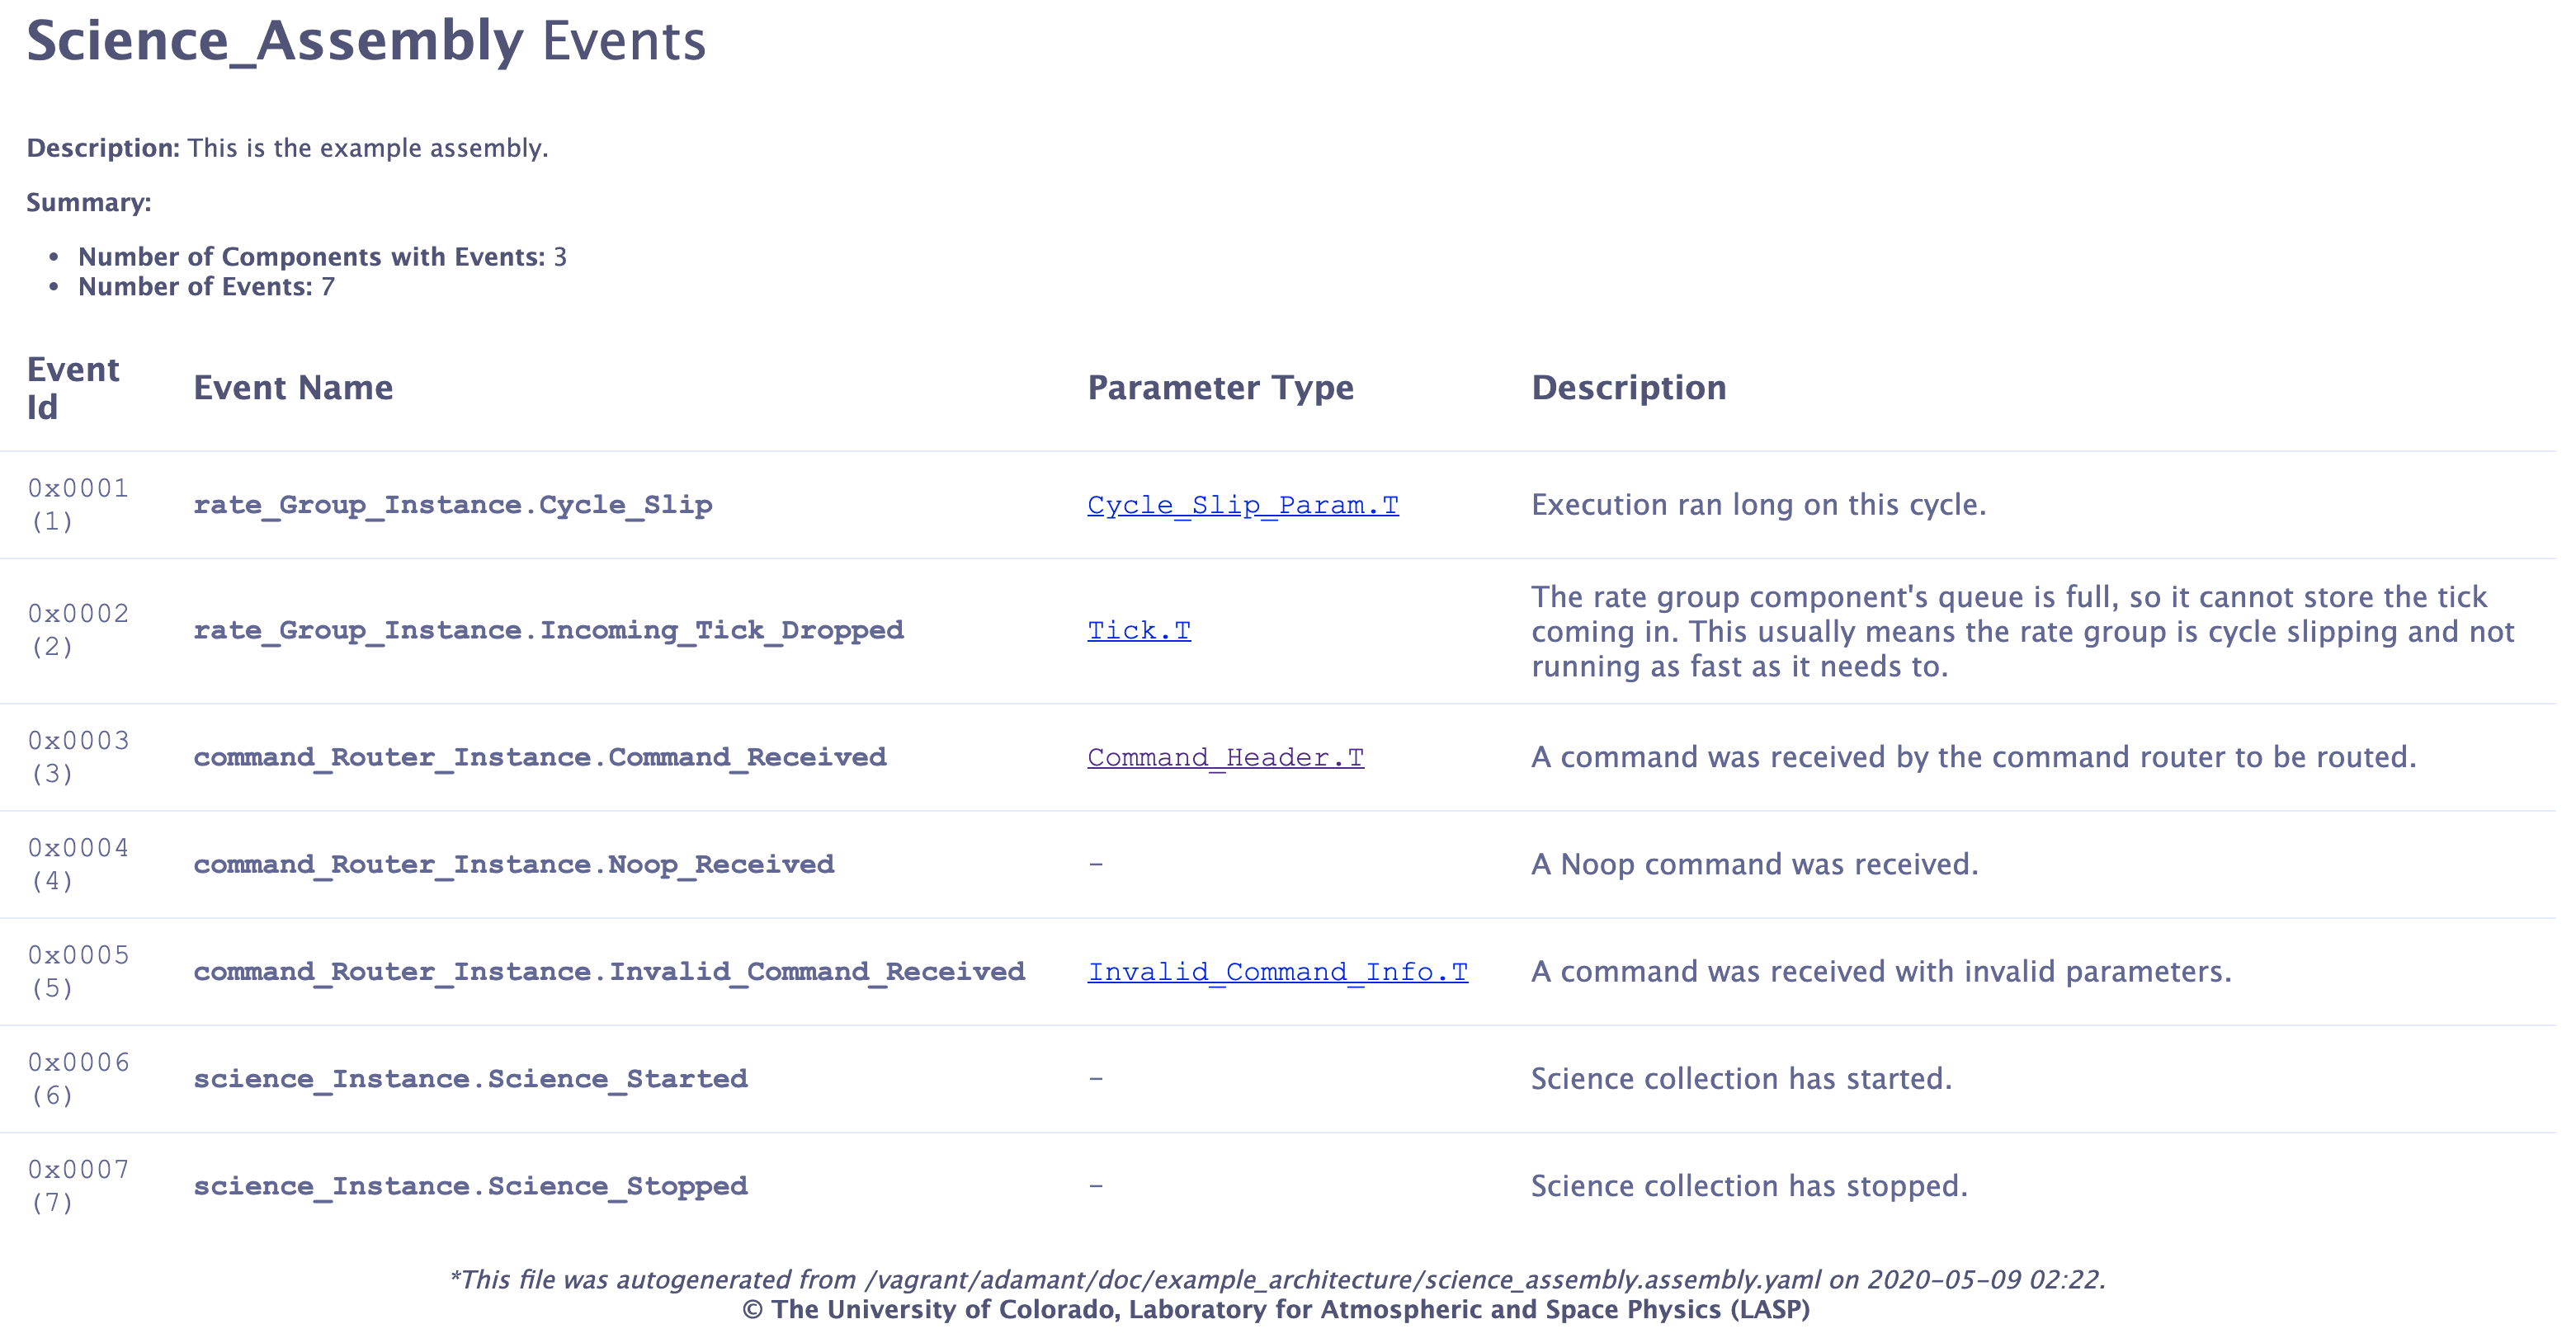
\includegraphics[width=\textwidth]{images/assemblyeventshtml.png}
\vspace{5mm} %5mm vertical space

Note that the analogous build rules exist for commands, parameters, data products, packets, and faults as well.

\subsection{Assembly Views} \label{Assembly Views}

Assembly diagrams, Section \ref{Creating an Assembly Diagram}, can get complex and hard to understand as more components and connections are added. In order to provide a more digestible way of consuming the information in an assembly model, the concept of assembly \textit{views} is introduced. A view is a diagram that only shows a subset of the entire assembly model in order to demonstrate a particular point to a set of stakeholders. Because a view is focused, and not cluttered by information that may distract from its main message, it is usually more adept at presenting certain aspects of the architecture. A collection of views can generally communicate architectural ideas much more effectively than an entire assembly diagram, making for more relevant discussions and more valuable design reviews. \\

Assembly diagrams in Adamant are directed graphs. For visualization Adamant uses \href{https://www.graphviz.org/}{\textcolor{blue}{Graphviz}}, in particular the \href{https://graphviz.gitlab.io/_pages/doc/info/lang.html}{\textcolor{blue}{DOT language}} language which excels at presenting directed graphs. \\

\subsubsection{Creating a View Model}

A view is specific to the assembly it is associated with. A view model can be thought of a ``graph filter" for the assembly. Imagine the entire, complex assembly graph. We will be working with the \textit{science\_assembly} diagram that was generated in Section \ref{Creating an Assembly Diagram}. The diagram is shown again below for reference.

\vspace{5mm} %5mm vertical space
\includegraphics[width=1.0\textwidth,center]{../example_architecture/build/eps/science_assembly.eps}
\vspace{5mm} %5mm vertical space

Using a view model, we can apply \texttt{filter}s to this diagram to limit what is shown. When the view filter's are applied, many components and connections are removed, leaving a subgraph that displays the desired ``view" of the assembly. The view model provides many mechanisms that allow filtering of the assembly graph, which will be presented in this section. \\

Creating views in Adamant is achieved using a \textit{view} model. To create a view for \textit{science\_assembly}, we simply need to name the view model appropriately. View models will always be of the form \textit{view\_name.assembly\_name.view.yaml} where \textit{view\_name} is the name of the specific view and \textit{assembly\_name} is the name of the assembly that the view applies to. Note that there is no limit to how many view models can be created for an assembly. \\

Usually it is best to create view models in their own subdirectory under the assembly directory. We begin by creating a \textit{views} directly:

\vspace{5mm} %5mm vertical space
\begin{minted}{text}
> mkdir views  # make views/ directory under science_assembly/
> cd views 
\end{minted}
\vspace{5mm} %5mm vertical space

In this directory we create our first view model named \textit{command\_view.science\_assembly.view.yaml}. The contents are shown below: \\

\textit{command\_view.science\_assembly.view.yaml:}
\yamlcodef{../example_architecture/command_view.science_assembly.view.yaml}

This YAML model file above contains comments explaining whether or not each field is optional or required. The model begins with an optional \texttt{description} of what the view shows. Using the optional \texttt{layout} tag, the developer can tell Graphvis the direction they would like the graph drawn. This is equivalent to setting the \href{https://www.graphviz.org/doc/info/attrs.html#d:rankdir}{\textcolor{blue}{\texttt{rankdir}}} attribute in Graphvis. The options for this tag are: \texttt{left-to-right}, \texttt{top-to-bottom}, \texttt{right-to-left}, or \texttt{bottom-to-top}. \\

Following is a set of \texttt{show\_*} switches. By default, if left unspecified, these tags are set to \texttt{True}. A description of each is shown below:

\vspace{5mm} %5mm vertical space
\begin{spaceditemize}
  \item \textbf{\texttt{show\_component\_type}} - Shows the component type name inside each component box.
  \item \textbf{\texttt{show\_component\_execution}} - Shows the component outlined in bold for active components and not outlined in bold for passive components.
  \item \textbf{\texttt{show\_component\_priority}} - Shows the component priority number inside each active component box.
  \item \textbf{\texttt{show\_component\_name}} - Shows the component instance name inside each component box.
  \item \textbf{\texttt{show\_connector\_type}} - Shows the connector type next to each connection.
  \item \textbf{\texttt{hide\_group\_outline}} - If set to \texttt{False}, it shows a dotted line around any ``groups" defined in the view
\end{spaceditemize}
\vspace{5mm} %5mm vertical space

Below the switches is the \texttt{rule} definition. Defining a rule is optional, and usually is not necessary. However, the rule feature gives a powerful way to define very specific subgraphs that otherwise would not be possible. It is easiest to describe rules after understanding \texttt{filters}, which will be described next. Rules are explained in Section \ref{Using View Rules}. In this case, the view only has a single filter, so a rule is unnecessary, since we just want to apply this filter to the assembly graph to produce our subgraph. \\

Below the \texttt{rule} definition is the \texttt{filters}. Any number of filters can be defined. Each filter takes the entire assembly graph as input and produces a subgraph as output. By default, if no rule is specified, the intersection of these subgraphs is taken in order to produce the view. That is, any shared connections and components that appear in ALL of the subgraphs is included in the view. \\

In this case we define a single \texttt{filter}. A \texttt{name} must be provided for the filter, and it must be unique within the view. A filter \texttt{type} must also be provided. Along with the filter type is one of two lists (but never both): an \texttt{include} list or an \texttt{exclude} list. If an \texttt{include} list is provided, then the assembly graph is filtered to \textit{include} any components or connections that meet the filter criteria to create the subgraph. If an \texttt{exclude} list is provided, then the assembly graph is filtered to include any components or connections that not NOT meet the filter criteria to create the subgraph. \\

There are two different types of view filters: 1) those that filter components, and 2) those that filter connectors. A component filter will remove any components that do not meet the filter criteria. Any connections that are shared between the components are left, and any connections that connect to removed components are pruned from the subgraph. The component filters are shown below:

\vspace{5mm} %5mm vertical space
\begin{spaceditemize}
  \item \textbf{\texttt{component\_name}} - Filter by component instance names, ie. \texttt{Command\_Router\_Instance}.
  \item \textbf{\texttt{component\_type}} - Filter by component type names, ie \texttt{Example\_Command\_Router}.
  \item \textbf{\texttt{component\_execution}} - Filter by component execution, either \texttt{active} or \texttt{passive}.
  \item \textbf{\texttt{component\_name\_context}} - Keep (or remove in the case of an \texttt{exclude} list) all components that have immediate connections with the specified component instances.
  \item \textbf{\texttt{component\_type\_context}} - Keep (or remove in the case of an \texttt{exclude} list) all components that have immediate connections with the specified component types.
\end{spaceditemize}
\vspace{5mm} %5mm vertical space

A connector filter will remove any connectors that do not meet the filter criteria. If any connector of a connection is filtered out, then both connectors of the connection are filtered out. After all the connections are removed, any component that is left with no connections to another component is also pruned. The connector filters are shown below:

\vspace{5mm} %5mm vertical space
\begin{spaceditemize}
  \item \textbf{\texttt{connector\_name}} - Filter by connector name in the form \texttt{\url{component\_instance\_name.connector\_name}}.
  \item \textbf{\texttt{connector\_type}} - Filter by connector type ie. something like \texttt{Command.T}.
  \item \textbf{\texttt{connector\_kind}} - Filter by connector kind, ie. \texttt{recv\_async}, \texttt{recv\_sync}, \texttt{send}, \texttt{request}, \texttt{service}, \texttt{get}, \texttt{return}, \texttt{provide}, or \texttt{modify}
\end{spaceditemize}
\vspace{5mm} %5mm vertical space

In this case we use the \texttt{connector\_type} filter type with an \texttt{include} list. In this way we are trying to include any connectors that are of type \texttt{Command.T}. Any components that do not have a \texttt{Command.T} connector will be removed. \\

The presence of the view model allows Adamant to provide new build rules:

\vspace{5mm} %5mm vertical space
\begin{minted}{text}
> redo what
redo  what
redo all
redo clean
redo clean_all
redo templates
redo publish
redo targets
redo prove
redo analyze
redo style
redo pretty
redo test_all
redo coverage_all
redo build/dot/science_assembly_command_view.dot
redo build/eps/science_assembly_command_view.eps
redo build/png/science_assembly_command_view.png
redo build/svg/science_assembly_command_view.svg
\end{minted}
\vspace{5mm} %5mm vertical space

As can be seen there is a rule to build diagrams as \texttt{.eps}, \texttt{.svg}, or \texttt{.png}. Each of these diagrams will also build the \texttt{.dot} file which is autocoded Graphvis DOT language that describes the graph. \\

The most convenient to build usually the \texttt{.svg} which can be built with:

\vspace{5mm} %5mm vertical space
\begin{minted}{text}
> redo build/svg/science_assembly_command_view.svg
\end{minted}
\vspace{5mm} %5mm vertical space

When opened in your favorite web browser the view will look like:

\begin{figure}[H]
  \includegraphics[width=1.0\textwidth,center]{../example_architecture/build/eps/science_assembly_command_view.eps}
\end{figure}

As expected, we see a view that only shows the command paths of the architecture. \\

Building a view based on connector types of interest is a very common way to construct views. Another common pattern is construct a view around a single component of interest. For this we can use the \texttt{component\_name\_context} filter which will create a subgraph of the component and only its immediate connections. \\

\textit{parameters\_context\_view.science\_assembly.view.yaml:}
\yamlcodef{../example_architecture/parameters_context_view.science_assembly.view.yaml}

The above YAML produces the following view, which shows how the \texttt{parameters\_Instance} is situated in the assembly.

\begin{figure}[H]
  \includegraphics[width=1.0\textwidth,center]{../example_architecture/build/eps/science_assembly_parameters_context_view.eps}
\end{figure}

\subsubsection{Using View Rules} \label{Using View Rules}

Now let's create some views that demonstrate the power of view \texttt{rules}. A \texttt{rule} tells Adamant how to apply the \texttt{filter}s specified in a view model. Defining a rule uses a simple language with the following operands.

\vspace{5mm} %5mm vertical space
\begin{spaceditemize}
  \item \textbf{\texttt{\&}} - Perform an \textit{intersection}, or \textit{and}, between the two subgraphs. Only components and connections found in both subgraphs will be included in the resulting subgraph.
  \item \textbf{\texttt{|}} - Perform a \textit{union}, or \textit{or}, between the two subgraphs. Any components and connections in the subgraphs will be combined together to form a larger subgraph which contains both.
  \item \textbf{\texttt{\textasciitilde{}}} - Perform a \textit{not} operation on the subgraph. The resulting subgraph will contain only components and connections not included in the input.
  \item \textbf{\texttt{()}} - Parenthesis can be used to enforce order of operations.
  \item \textbf{\texttt{@}} - Define the included subgraph as a ``group" which will be graphed independently of the rest of the view. See Section \ref{Configuring View Graph Layout} for more details.
\end{spaceditemize}
\vspace{5mm} %5mm vertical space

For clarity a few rules are written below and explained in English:

\vspace{5mm} %5mm vertical space
\begin{spaceditemize}
  \item \textbf{\texttt{f1 \& \textasciitilde{}f2}} - Perform an \textit{and} operation, or \textit{intersection}, between the subgraphs created by filter \texttt{f1} and the subgraph created by the \textit{not} of filter \texttt{f2}. The \textit{not} of \texttt{f2} will include every component and connection not included in the subgraph created by \texttt{f2}.
  \item \textbf{\texttt{f3 \& (f1 | f2)}} - Perform an \textit{and}, \textit{intersection}, between the two subgraphs \texttt{f3} and the subgraph resulting from the \textit{or}, \textit{union}, of \texttt{f1} and \texttt{f2}.
  \item \textbf{\texttt{@f3 | f1}} - Perform an \textit{or}, \textit{union}, between \texttt{f3} and \texttt{f1}. When producing the graph, graph \texttt{f3} by itself as a Graphvis \textit{group} before adding the elements in \texttt{f1}. See Section \ref{Configuring View Graph Layout} for more details.
\end{spaceditemize}
\vspace{5mm} %5mm vertical space

Let's demonstrate the use of rules with a few examples. First, consider the \textit{parameters\_context\_view.science\_assembly.view.yaml} view model that was created at the end of the last section. There are other ways to make this same view diagram with a different model. Consider the model file below. \\

\textit{parameters\_view.science\_assembly.view.yaml:}
\yamlcodef{../example_architecture/parameters_view.science_assembly.view.yaml}

In this case we create a large subgraph, created by filter \texttt{include\_component\_types}, that includes all the components that we are interested in. However, we do not want to show the \texttt{Command.T} connection from the \texttt{command\_Router\_Instance} to the \texttt{science\_Instance}. We remove this connection by \textit{and}ing \texttt{include\_component\_types} with the \texttt{exclude\_connector} filter, which creates a subgraph without the connector we want to remove. The resulting view is what we expect.

\begin{figure}[H]
  \includegraphics[width=1.0\textwidth,center]{../example_architecture/build/eps/science_assembly_parameters_view.eps}
\end{figure}

Note that this view would still work without specifying a \texttt{rule}. If left unspecified, the default rule is to \textit{and} all the filters together in order, which is exactly what we have specified manually here. \\

Let's try generating the same view in yet another way. This time we will use the \textit{or} operand. \\

\textit{parameters\_view2.science\_assembly.view.yaml:}
\yamlcodef{../example_architecture/parameters_view2.science_assembly.view.yaml}

We create two subgraphs from the two filters. \texttt{include\_param\_connectors} creates a subgraph that includes any \texttt{Parameter.T} typed connections. This only applies to two components, \texttt{parameters\_Instance} and \texttt{science\_Instance}. The \texttt{include\_parameter\_command} filter simply creates a subgraph with the two components \texttt{command\_Router\_Instance} and \texttt{parameters\_Instance}. We then combine, via \textit{or}, the two subgraphs together to create the desired view:

\begin{figure}[H]
  \includegraphics[width=1.0\textwidth,center]{../example_architecture/build/eps/science_assembly_parameters_view2.eps}
\end{figure}

Finally, to demonstrate the \textit{not} rule operand, see the following model file. In this case we are trying to create a view that contains everything but the \texttt{command\_Router\_Instance} and \texttt{parameters\_Instance}. One way to do this is to create a filter that includes both of these components and then use the \textit{not} operator to invert it. \\

\textit{no\_command\_params.science\_assembly.view.yaml:}
\yamlcodef{../example_architecture/no_command_params.science_assembly.view.yaml}

The \texttt{rule} creates the view that we wanted.

\begin{figure}[H]
  \includegraphics[width=1.0\textwidth,center]{../example_architecture/build/eps/science_assembly_no_command_params.eps}
\end{figure}

\subsubsection{Configuring View Graph Layout} \label{Configuring View Graph Layout}

When creating views, sometimes the resulting computer-generated graph is not exactly how you imagined it looking. While you cannot drag and drop components and connections into different locations, Adamant does provide a few ways to tweak the layout of a graph to make it more presentable. \\

The first tool we will talk about is a \texttt{rule} operand for creating subgraph \textit{groups} using the \texttt{@} symbol. Note this operand uses the underlying \href{https://www.graphviz.org/doc/info/attrs.html#d:clusterrank}{\textcolor{blue}{\texttt{subgraph cluster}}} feature of the DOT language. \\

\textit{grouped\_view.science\_assembly.view.yaml:}
\yamlcodef{../example_architecture/grouped_view.science_assembly.view.yaml}

Note that we used quotes around the rule to make it valid YAML. The YAML schema will complain if a value begins with \texttt{@}. \\

In this view model we combine the subgraphs of two filters together using \textit{or} and we tell Adamant to create a \textit{group} out of the first subgraph. The resulting view looks like:

\begin{figure}[H]
  \includegraphics[width=1.0\textwidth,center]{../example_architecture/build/eps/science_assembly_grouped_view.eps}
\end{figure}

As can be seen, there appears to be two graphs drawn that are connected together. The first graph is centered around the \texttt{science\_Instance} and the second is centered around the \texttt{command\_Router\_Instance}. In this way, a user can use this feature to better organize their views. \\

Adamant also provides features that allow for the insertion of inline DOT at the beginning or end of the generated DOT file using the \texttt{preamble} and \texttt{postamble} tags, respectively. Any DOT code can be specified found in the \href{https://graphviz.gitlab.io/_pages/doc/info/lang.html}{\textcolor{blue}{DOT language specification}}. \\

Most commonly, in Adamant, you will use the \texttt{postamble} tag to specify the \texttt{rank} of different components in the view graph. Specifying rank attributes allows us to change where components are drawn in the diagram. To demonstrate, we create a view that uses the \texttt{rank} attribute to make a cleaner version of the \textit{science\_assembly} diagram. No components or connections are filtered out in this case. \\

\textit{science\_assembly\_view.science\_assembly.view.yaml:}
\yamlcodef{../example_architecture/science_assembly_view.science_assembly.view.yaml}

which produces the view:

\begin{figure}[H]
  \includegraphics[width=1.0\textwidth,center]{../example_architecture/build/eps/science_assembly_science_assembly_view.eps}
\end{figure}

For this view model we specified 3 components at the \textit{sink rank}. This tells Graphvis to draw the graph with these three components on the far right, one on top of the other. The resulting view is nice, compact, and easy to understand. Note that when using this feature you MUST spell the component instance names exactly correct, including the correct capitalization, otherwise an error or odd looking view will result. \\

More than one rank and group can be specified by adding another set of ``\{\}" with DOT inside. Other useful rank values include \textit{source}, which is the opposite of \textit{sink}, and \textit{same} which groups the specified components at the same level in the graph. \\

For more information on DOT rank specifications see \href{https://www.graphviz.org/doc/info/attrs.html#d:rank}{\textcolor{blue}{this documentation}}. \\

Creating good view diagrams takes practice and trial and error. Often you will need to create the view, see how it looks, and then slowly make adjustments until it looks the way you want. For more examples, take a look at the \href{https://github.com/lasp/adamant_example/tree/main/src/assembly/linux/views}{\textcolor{blue}{example repository views}}.

\subsection{Assembly Documentation} \label{Assembly Documentation}

One of the benefits of the extensive modeling required by Adamant is that rich, informative documentation can be generated with little extra effort. This documentation is beneficial at all stages of the development process, from working out the details of the design, to reviewing the implementation. \\

It is advisable to generate assembly documentation as soon as a solid assembly model has been developed for a system. In this way, the document can be used to explain the design to other engineers and gain feedback before the implementation has even begun. During the development process, the design document should periodically be regenerated to reflect any changes. Finally, when the assembly is complete, the design document should be reviewed to ensure that it contains all the information necessary for another engineer to use or make changes to the design. Sometimes this requires adding custom sections to the design document that the document autocoder would not be able to create on its own. \\

This section walks through how to generate documentation for assemblies.

\subsubsection{Assembly HTML}

Adamant provides some handy HTML tables for collating assembly design information. Some of the most useful HTML products were described for assembly IDed entities in Section \ref{IDed Entity Documentation}. In addition, the following rules are provided, using the \textit{science\_assembly} as and example: \\

Show information about all components in assembly: \\
\begin{minted}{text}
> redo build/html/science_assembly_components.html
\end{minted}
\vspace{7mm} %5mm vertical space

Show information about all connections in assembly: \\
\begin{minted}{text}
> redo build/html/science_assembly_connections.html
\end{minted}
\vspace{7mm} %5mm vertical space

Show information about all interrupts in an assembly: \\
\begin{minted}{text}
> redo build/html/science_assembly_interrupts.html
\end{minted}
\vspace{7mm} %5mm vertical space

Show information about all tasks and their priorities: \\
\begin{minted}{text}
> redo build/html/science_assembly_priorities.html
\end{minted}
\vspace{7mm} %5mm vertical space

Show information about all queued components: \\
\begin{minted}{text}
> redo build/html/science_assembly_queues.html
\end{minted}
\vspace{7mm} %5mm vertical space

Below are some of sample outputs using the \textit{science\_assembly}. \\

\textit{science\_assembly\_components.html:} \\

\includegraphics[width=\textwidth]{images/assemblycomponentshtml.png}
\vspace{7mm} %5mm vertical space

\textit{science\_assembly\_connections.html:} \\

\includegraphics[width=\textwidth]{images/assemblyconnectionshtml.png}
\vspace{7mm} %5mm vertical space

\textit{science\_assembly\_priorities.html:} \\

\includegraphics[width=\textwidth]{images/assemblyprioritieshtml.png}
\vspace{7mm} %5mm vertical space

\textit{science\_assembly\_queues.html:} \\

\includegraphics[width=\textwidth]{images/assemblyqueueshtml.png}
\vspace{7mm} %5mm vertical space

\subsubsection{Assembly Design Document}

One of the benefits of the extensive modeling required by Adamant is that rich, informative documentation can be generated with little extra effort. To generate documentation for an assembly, an assembly model must first exist. This section demonstrates how to generate documentation for the \textit{science\_assembly} that has been discussed in previous sections. Generating documentation for an assembly follows the same pattern as generating documentation for a component, which is discussed in Section \ref{Component Design Document}. \\

Assembly documentation must be generated and stored in a subdirectory \textit{doc/} of the assembly's main directory. In fact, Adamant only produces rules to build assembly documentation within a \textit{doc/} directory. This convention makes it easy to locate the documentation for any assembly in the repository. \\

To create documentation for the \textit{science\_assembly} we first create the doc directory:

\vspace{5mm} %5mm vertical space
\begin{minted}{text}
> mkdir doc  # make doc/ directory under science_assembly/
> cd doc
\end{minted}
\vspace{5mm} %5mm vertical space

After we are inside the new \textit{doc/} directory we can view the build rules that are available.

\vspace{5mm} %5mm vertical space
\begin{minted}{text}
> redo what
redo  what
redo all
redo clean
redo clean_all
redo templates
redo publish
redo targets
redo prove
redo analyze
redo style
redo pretty
redo test_all
redo coverage_all
redo build/pdf/science_assembly_commands.pdf
redo build/pdf/science_assembly_components.pdf
redo build/pdf/science_assembly_connections.pdf
redo build/pdf/science_assembly_data_products.pdf
redo build/pdf/science_assembly_description.pdf
redo build/pdf/science_assembly_enums.pdf
redo build/pdf/science_assembly_events.pdf
redo build/pdf/science_assembly_packets.pdf
redo build/pdf/science_assembly_priorities.pdf
redo build/pdf/science_assembly_stats.pdf
redo build/pdf/science_assembly_types.pdf
redo build/pdf/science_assembly_views.pdf
redo build/template/science_assembly.tex
redo build/tex/science_assembly_commands.tex
redo build/tex/science_assembly_components.tex
redo build/tex/science_assembly_connections.tex
redo build/tex/science_assembly_data_products.tex
redo build/tex/science_assembly_description.tex
redo build/tex/science_assembly_enums.tex
redo build/tex/science_assembly_events.tex
redo build/tex/science_assembly_packets.tex
redo build/tex/science_assembly_priorities.tex
redo build/tex/science_assembly_stats.tex
redo build/tex/science_assembly_types.tex
redo build/tex/science_assembly_views.tex
\end{minted}
\vspace{5mm} %5mm vertical space

As can be seen, there are many different \textit{.tex} files that can be created, each that can be used to produce a small PDF stub of that piece of documentation. Most importantly there is a rule to build the documentation template, which is the master \LaTeX{} file for the assembly documentation. To build and use the template we run:

\vspace{5mm} %5mm vertical space
\begin{minted}{text}
> redo build/template/science_assembly.tex
> cp build/template/* .  # copy the template file into doc/
\end{minted}
\vspace{5mm} %5mm vertical space

This template provides an excellent start to our assembly documentation and often provides sufficient detail to be used without modification. However, like all template files in Adamant, this is meant to be modified, if necessary, to add additional hand-written documentation. Let's take a look at the autogenerated \textit{science\_assembly.tex} file. \\

\textit{science\_assembly.tex:}
\latexcodef{../example_architecture/doc/science_assembly.tex}

As can be seen, this file defines the sections of the assembly documentation and imports most of the text from external autogenerated \textit{.tex} files. Feel free to modify this file to add extra sections to the assembly documentation. \\

To generate a PDF from this file run:

\vspace{5mm} %5mm vertical space
\begin{minted}{text}
> redo build/pdf/science_assembly.pdf
\end{minted}
\vspace{5mm} %5mm vertical space

By default, PDF files are generated in the \textit{build/pdf/} directory. This allows the developer to review the output documentation before ``publishing" it, ie. saving it in the repository. Once the documentation looks good, you can publish it manually by copying it into the \textit{doc/} directory:

\vspace{5mm} %5mm vertical space
\begin{minted}{text}
> cp build/pdf/science_assembly.pdf .
\end{minted}
\vspace{5mm} %5mm vertical space

or alternatively you can run the special Adamant command:

\vspace{5mm} %5mm vertical space
\begin{minted}{text}
> redo publish
\end{minted}
\vspace{5mm} %5mm vertical space

which will build the documentation and perform the copy for you. Note that any assembly views, Section \ref{Assembly Views}, found in subdirectories of the model directory will automatically be added to the documentation with a caption that matches the view's description. \\

The produced documentation is not shown here for brevity, but is linked \href{https://github.com/lasp/adamant/blob/main/doc/example_architecture/doc/science_assembly.pdf}{\textcolor{blue}{here}}. For a more complete example, check out the \href{https://github.com/lasp/adamant_example/blob/main/src/assembly/linux/doc/linux_example.pdf}{\textcolor{blue}{example repository assembly design document}}.

\subsection{Assembly Metrics}

Since an executable assembly is usually used to build the final production binary for a project, it is often valuable to keep track of certain code metrics such as the number of lines of code, packages, files, etc. for each assembly. Adamant provides the ability to generate metrics for any executable produced in the system. Steps to produce different metrics for any file, object, or binary in Adamant is discussed in Section \ref{Code Metrics}. The same example there can be applied for an assembly binary to produce the SLOC and other metrics of interest for a final executable.

\subsection{Assembly Ground System Integration}

When an assembly is compiled into an executable binary and deployed to the target embedded system, often the only way to communicate with it is through some external system. In the domain of spacecraft flight software, this communication system is the ground. Since Adamant is model driven and generators can be constructed to produce any desired output, see Section \ref{Adding Generators}, it is conceivable that any ground system can be supported. Currently there is support for integration with the LASP-developed ground system Hydra, which is presented in this section.

\subsubsection{Hydra Integration}

\textit{Note that Hydra is not yet publicly available, but will be made so in the future.}

Adamant provides support for interfacing with Hydra at the assembly level. Specifically, any assembly can be controlled by Hydra via commands and receive data from the Adamant system through data products and packets. \\

Hydra is configured via special XML files. Many of these files can be generated from an Adamant assembly model. To see what is available we can run \texttt{redo what} from an assemnbly directory. For example, we can run this from the \textit{science\_assembly} directory created in previous sections (some output omitted for brevity):

\vspace{5mm} %5mm vertical space
\begin{minted}{text}
> redo what
redo  what
redo all
redo clean
redo clean_all
redo templates
redo publish
redo targets
redo prove
redo analyze
redo style
redo pretty
redo test_all
redo coverage_all
redo build/hydra/Config/science_assembly.xml
redo build/hydra/Config/science_assembly_ccsds_commands.xml
redo build/hydra/Config/science_assembly_ccsds_packets.xml
redo build/hydra/Pages/science_assembly_cpu_monitor.xml
redo build/hydra/Pages/science_assembly_queue_monitor.xml
redo build/hydra/Pages/science_assembly_stack_monitor.xml
redo build/hydra/Scripts/science_assembly_packet_pages.prc
\end{minted}
\vspace{5mm} %5mm vertical space

As can be seen, all hydra configuration files are created in subdirectories of \textit{build/hydra}. The subdirectory names map to the standard Hydra configuration file structure. \\

The \textit{science\_assembly.xml} file is the main Hydra configuration file. It includes definitions for all the types, data products, events, etc. that are defined in the assembly. The \textit{science\_assembly\_ccsds\_commands.xml} and \textit{science\_assembly\_ccsds\_packets.xml} files are created from special generators for the \texttt{CCSDS\_Command\_Depacketizer} and \texttt{CCSDS\_Packetizer} components, respectively (\textit{src/components/CCSDS}). They add CCSDS support to Hydra for sending commands and receiving LASP formatted CCSDS packets. \\

Next, we can see that 3 Hydra pages can be generated for viewing packets from the Adamant monitor components (\textit{src/components/monitors}). \\

Lastly, Adamant can generate the \textit{science\_assembly\_packet\_pages.prc} script which automatically generates pages for every packet that an assembly can produce. \\

Coordinating these autocoded files into a fully functional Hydra configuration is too complicated to describe in this document. However, a fully functional example is provided in the example repository \href{https://github.com/lasp/adamant_example/tree/main/src/assembly/linux/main/hydra}{\textcolor{blue}{hydra configuration directory}}. Hydra can be spawned and interfaced with the \texttt{Linux} assembly by running the single command:

\vspace{5mm} %5mm vertical space
\begin{minted}{text}
> redo run_with_hydra
\end{minted}
\vspace{5mm} %5mm vertical space

from \textit{src/assembly/Linux/main} within the example repository. \\

By digging into the example project Hydra configuration you can explore how it works and adapt it for your own system, or translate it for a different ground system.

\newpage
\section{Ground Tools} \label{Ground Tools}

The ground-based testing and analysis tools included with Adamant are in their infancy. Current ground-based tools are powered by the autocoded python classes that can be generated for any packed type found in the software, see Section \ref{Packed Record Python Class}. Since Adamant has a way to decode/encode any data that comes from or needs to go to the Adamant-based embedded system, a myriad of tools can be produced. The current tools available can be found in \textit{gnd/}. Included are tools for decomming events from a post mortem log and from a socket, as well as a tool for analyzing CCSDS packets and reporting errors. This section of the User Guide will be expanded when Adamant's ground tools become more extensive and mature.

Recently, support for a MATLAB version of the python tools have been added and can be found in \textit{gnd/matlab}. These tools rely on autocoded \texttt{.m} files for Adamant packed records, in the same way the that the python tools rely on autocoded \texttt{.py} files for Adamant packed records.

\newpage
\section{Advanced Topics}

This section provides discussion on various advanced usages of Adamant. These topics are not necessarily ``hard" to understand. However, the features presented are not as commonly used as those presented in other sections. Knowledge of this section is often only required by one member of a team using Adamant. Where appropriate, the sections above link to sections here to provide additional information.

\subsection{Interfacing with C and C++} \label{C Interfacing}

Ada includes extensive facilities to support multi-language development. See, \href{https://learn.adacore.com/courses/intro-to-embedded-sys-prog/chapters/multi_language_development.html}{\texttt{\textcolor{blue}{AdaCore Learn}}} for specific details. In Adamant, we have formalized Ada calling into external C or C++ libraries and provided some tooling to make this easier. Note, this assumes Ada is still being used as the \textit{main program}. If you would rather learn by example see the \texttt{c\_demo} or \texttt{cpp\_demo} components in the \textit{example repository}. \\

To include a C or C++ library we must first include the library in the Adamant build path, just like we would with Ada source code, ie.

\vspace{5mm} %5mm vertical space
\begin{minted}{text}
> cd c_lib
> ls -a c_lib
.  ..  .all_path  c_lib.c  c_lib.h
\end{minted}
\vspace{5mm} %5mm vertical space

The Adamant build system recognizes that there are C files in this repository because they are named \textit{.h} and \textit{.c}. C++ files should be named \textit{.hpp} and \textit{.cpp} to be recognized by Adamant. Running \texttt{redo what} shows us that we can compile the C files, as well as generate automatic Ada bindings to call into this C library.

\vspace{5mm} %5mm vertical space
\begin{minted}{text}
> redo what
redo  what
redo all
redo clean
redo build/obj/Linux/c_lib.o
redo build/template/Linux/c_lib_h.ads
\end{minted}
\vspace{5mm} %5mm vertical space

Note that binding generation is specific to your build target, since different compilers will often bind to symbols with different naming. To build the Ada bindings run:

\vspace{5mm} %5mm vertical space
\begin{minted}{text}
> redo templates
  redo  templates
  redo    build/template/Linux/c_lib_h.ads
\end{minted}
\vspace{5mm} %5mm vertical space

Let's take a look at the C source code: \\

\textit{c\_lib.h}:
\ccodef{../example_architecture/c_lib/c_lib.h}

\textit{c\_lib.c}:
\ccodef{../example_architecture/c_lib/c_lib.c}

which provides a simple data structure and function that increments a value up to a limit before rolling over. Let's also look at the generated Ada bindings: \\

\textit{c\_lib\_h.ads}:
\adacodef{../example_architecture/c_lib/build/template/Linux/c_lib_h.ads}

As you can see, \textit{c\_lib\_h.ads} includes Ada bindings for the C struct and the call to \texttt{increment}. Below is an example \textit{main.adb} that uses the bindings to call the C library. \\

\textit{main.adb}:
\adacodef{../example_architecture/c_lib/main.adb}

The same pattern described above works for C++ libraries except the binding file would be named \textit{<cpp\_lib\_name>\_hpp.ads}. Note that these files are provided as templates because it is quite likely that you may want to tweak these files to fit your specific usage of the C/C++ library. At the very least, the templates can give you a big head start. \\

If the naming convention, \textit{<c\_lib\_name>\_h.ads} for C libraries and \textit{<cpp\_lib\_name>\_hpp.ads} for C++ libraries, is used, then the Adamant build system will be able to automatically build both the Ada and C/C++ and link them together. If you deviate from this convention, you are on your own, and you may need to write custom \textit{.do} files to get everything to compile and link appropriately. \\

More advanced patterns, like having the C/C++ call back into Ada, are possible but are not discussed here. See \href{https://learn.adacore.com/courses/intro-to-embedded-sys-prog/chapters/multi_language_development.html}{\texttt{\textcolor{blue}{AdaCore Learn}}} if the pattern presented above does not meet your needs.

\subsection{IDE Integration} \label{IDE Integration}

Adamant has been designed to not depend on any particular Integrated Development Environment (IDE) for development. Since interaction with the system is provided via a commandline interface, developers can choose to use any editor or IDE to develop code for Adamant. Modern IDEs provide much in terms of helping the developer, from push-button compilation to code block suggestions. Full integration of Adamant with an Ada-equipt IDE is on the framework roadmap, however some work in the vein has already been completed. \\

Most Ada IDEs require the use of a central \textit{.gpr} project file in order to determine the source code and settings for a project. Since Adamant uses a custom \texttt{redo}-based build system, it does not require a project file in the same form. However, to allow easy integration of Adamant within an IDE, a \textit{.gpr} file can be produced for any binary (\textit{test.adb} or \textit{main.adb}) that can be compiled in the system. For example, if you run:

\vspace{5mm} %5mm vertical space
\begin{minted}{text}
> redo build/gpr/test.gpr
\end{minted}
\vspace{5mm} %5mm vertical space

from a unit test directory or 

\vspace{5mm} %5mm vertical space
\begin{minted}{text}
> redo build/gpr/main.gpr
\end{minted}
\vspace{5mm} %5mm vertical space

from the project main directory, a \textit{.gpr} file will be produced that can be opened with an Ada-enabled IDE such as \href{https://docs.adacore.com/live/wave/gps/html/gps_ug/index.html}{\textcolor{blue}{GNAT Studio}}. As an example, running \texttt{redo built/gpr/main.gpr} from the \textit{simple\_package} unit test directory produces the following \textit{.gpr} file: \\

\textit{simple\_package/test/build/gpr/test.gpr}:
\textcodef[breaklines=false]{../example_architecture/simple_package/test/build/gpr/test.gpr}

Opening this file with an IDE will allow you to view and modify any source code used to generate the unit test binary.

\subsection{Coding Style} \label{Coding Style}

A coding style is a set of rules or guidelines used when writing the source code for a program. The rules generally pertain to the visual appearance of the code and the aim is to improve uniformity in the ``look" of the code. Once developers become accustomed to a particular coding style, they can more easily read and understand source code written in that style. Adamant enforces a coding style for all Ada, Python, and YAML to enforce consistency and improve understandability. \\

The main tool for enforcing style is \texttt{redo style}. When run, this will check any Ada, Python, YAML, or autocoded Ada, Python, or YAML and ensure that the style guidelines are met. The following example is run in \textit{doc/example\_architecture/style\_demo}. Which includes the following poorly written code: \\

\textit{main.adb}:
\adacodef{../example_architecture/style_demo/main.adb}

\textit{main.py}:
\pythoncodef{../example_architecture/style_demo/main.py}

\textit{component\_model\_to\_lint.component.yaml}:
\yamlcodef{../example_architecture/style_demo/component_model_to_lint.component.yaml}

We can run \texttt{redo style} on this code to see what lines of code are problematic:

\vspace{5mm} %5mm vertical space
\begin{minted}{text}
> redo style
\end{minted}
\inputminted{text}{../example_architecture/style_demo/build/style/style.log}
\vspace{5mm} %5mm vertical space

The example above shows style warnings found for an Ada source file \textit{main.adb}, a Python source file \textit{main.py}, and a YAML model file \textit{component\_model\_to\_lint.component.yaml}. Style warnings are printed to the terminal and also stored in \textit{build/style/style.log}. \\

The warnings can be removed by manually correcting the code to meet the standard. However, this can become cumbersome if there are many warnings. To aid in this process, Adamant provides the special command \texttt{redo pretty} which will ``pretty" format any source code found in the current directory. Currently \texttt{redo pretty} only supports Ada and Python code, not YAML. Newly formatted code will be produced in \textit{build/pretty} and will adhere to the coding style.

\vspace{5mm} %5mm vertical space
\begin{minted}{text}
> redo pretty
\end{minted}
\inputminted{text}{../example_architecture/style_demo/output3.txt}
\vspace{5mm} %5mm vertical space

This will produce properly formatted Ada and Python versions of any code found in the current directory or autocoded in \textit{build/src} or \textit{build/py}. \\

The Adamant Ada coding style is based on style rules for the GNAT Ada compiler source code. Small modifications to this standard have been made to enforce some rules deemed important for writing safety critical software. Others rules have been loosened where the style was deemed overly strict, especially in regard to the style of comments. Examples of the Adamant coding style can be seen wherever the Ada programming language is reproduced in this User Guide. The coding style is enforced during compilation via the \texttt{-gnatyx} switch. The available style options are documented \href{https://gcc.gnu.org/onlinedocs/gnat_ugn/Style-Checking.html}{\textcolor{blue}{here}}. Adamant uses the following configuration checking coding style: \texttt{-gnaty3aABbdDefhiklL12nOprStux}. To format proper Ada, \texttt{redo pretty} utilizes the Ada pretty printer tool \href{https://gcc.gnu.org/onlinedocs/gcc-4.3.2/gnat_ugn_unw/The-GNAT-Pretty_002dPrinter-gnatpp.html}{\textcolor{blue}{gnatpp}}. \\

The Adamant Python coding style adheres to \href{https://peps.python.org/pep-0008/}{\textcolor{blue}{PEP 8}}. Adherence to the standard via \texttt{redo style} is provided by \href{https://flake8.pycqa.org/en/latest/}{\textcolor{blue}{flake8}}. To format proper looking Python, \texttt{redo pretty} utilizes \href{https://black.readthedocs.io/en/stable/index.html}{\textcolor{blue}{black}}. \\

Adamant YAML style is enforced when running \texttt{redo style} by \href{https://yamllint.readthedocs.io/en/stable/}{\textcolor{blue}{yamllint}}. \\

By default, coding style checks are not performed when compiling Ada source code, only when running \texttt{redo style}. However, these checks can be turned on while compiling by setting the appropriate environment variable.

\vspace{5mm} %5mm vertical space
\begin{minted}{text}
> export CHECK_STYLE=True
\end{minted}
\vspace{5mm} %5mm vertical space

This can be useful to ensure that all code you are currently working on and depending on meets the coding standard. \\

Using the \texttt{CHECK\_STYLE} variable will enforce style checks during every compile. If this becomes tiresome, you can disabled style checking by unsetting the variable:

\vspace{5mm} %5mm vertical space
\begin{minted}{text}
> export CHECK_STYLE=
\end{minted}
\vspace{5mm} %5mm vertical space

\subsection{Static Analysis} \label{Static Analysis}

Static analysis is the act of running code through a program to search for potential vulnerabilities or defects prior to compilation. Adamant provides support for static analysis through the \href{https://docs.adacore.com/codepeer-docs/users_guide/_build/html/index.html}{\textcolor{blue}{CodePeer}} tool developed by AdaCore. To make CodePeer easier to run on Adamant style code, it has been integrated into the build system and can be run via \texttt{redo} calls. The following sections outline how to run CodePeer locally, from a developer machine, and also on a remote server.

\subsubsection{Local Static Analysis}

To invoke CodePeer on a set of code simply run:

\vspace{5mm} %5mm vertical space
\begin{minted}{text}
> redo analyze
\end{minted}
\vspace{5mm} %5mm vertical space

from any directory. Adamant supports running CodePeer in two modes: a) \textit{library} mode and b) \textit{binary} mode. If \texttt{redo analyze} is run in a directory where a \textit{test.adb} or \textit{main.adb} is found, it will be run in \textit{binary} mode, otherwise it will be run in \textit{library} mode. In \textit{binary} mode, all source code found in the compiled binary is run through the CodePeer (except for test-only source code which is never analyzed). In \textit{library} mode, only the source code found (or generated) in the current directory is analyzed. Which mode is being utilized is printed in the output when running \textit{redo analyze}. \\

Consider the example code below:

\adacodef{../example_architecture/analyze_demo/main.adb}

The code above compiles with no warnings, but it has a defect that CodePeer can readily find. Let's run \texttt{redo analyze}.

\vspace{5mm} %5mm vertical space
\begin{minted}{text}
> redo analyze
\end{minted}
\inputminted{text}{../example_architecture/analyze_demo/output.txt}
\vspace{5mm} %5mm vertical space

From the output we can see that \texttt{redo analyze} was run in binary mode since this program is a \texttt{main.adb}. However, since the program only contains one file, only this single file is analyzed. From the results, we can see that a ``high" warning was produced for line 8, indicating that our out parameter might not be initialized. This pinpoints a defect in our code which is the \texttt{if} conditional that only sets the out parameter if the input is less than 20. Otherwise, the out parameter is left uninitialized, which could potentially cause problems for the rest of the program. \\

In fact, when running the program, this bug is very evident:

\vspace{5mm} %5mm vertical space
\begin{minted}{text}
> redo run 
\end{minted}
\inputminted{text}{../example_architecture/analyze_demo/output2.txt}
\vspace{5mm} %5mm vertical space

The old value of \texttt{Outer\_Var} is reported to be some random number that is not at all the value of 6 like we would expect. \\

CodePeer can be run in different configurations that analyze code at a deeper level, thus finding more potential errors, and also more false positives. This configuration is controlled via the CodePeer \texttt{Level} and \texttt{Messages} settings. \texttt{Level} can be configured to be a value between 0 and 4, where 4 performs the most thorough analysis, but also takes the longest time to complete. Information on the difference between the individual levels can be found \href{https://docs.adacore.com/codepeer-docs/users_guide/_build/html/running.html#codepeer-levels}{\textcolor{blue}{here}}. \texttt{Messages} is used to filter out messages that are more likely to be false positives. It can be set to \texttt{min}, \texttt{normal}, or \texttt{max}. A setting of \texttt{max} will show the most messages produced by CodePeer and show the most false positives. A setting of \texttt{min} will show only those messages most likely to indicate real defects. By default, \texttt{redo analyze} runs CodePeer with a setting of \texttt{-level=2} and \texttt{-messages=normal}. \\

These defaults can be changed by including a YAML file which alters the configuration for a particular directory. To do this we can add the file \textit{all.analyze.yaml}:

\yamlcodef{../example_architecture/analyze_demo/all.analyze.yaml}

In this case, running \texttt{redo analyze} in this directory will run CodePeer at \texttt{-level=1} and \texttt{-messages=min}.

\subsubsection{Static Analysis on Server}

On a large code base, running CodePeer with a high \texttt{level} setting can take many hours to complete. It is often ideal to employ CodePeer on a server with more resources to support nightly analysis runs, as described \href{https://docs.adacore.com/codepeer-docs/users_guide/_build/html/workflows.html#nightly-runs-on-a-server}{\textcolor{blue}{here}}. Analysis can be run using the directions provided in the previous section. \texttt{redo analysis} can easily be tied into any continuous integration process. \\

After analysis is run, the results can be viewed locally on a developer machine using the GNAT Studio IDE server. The server will provide the analysis results to a local running instance of the GNAT Studio IDE for viewing. This process is described \href{https://docs.adacore.com/codepeer-docs/users_guide/_build/html/viewing_output.html#accessing-results-remotely-ide}{\textcolor{blue}{here}}. Adamant provides a simple way to launch the IDE server. On the server machine, from the directory where \texttt{redo analyze} was run, run

\vspace{5mm} %5mm vertical space
\begin{minted}{text}
> redo codepeer_server
\end{minted}
\vspace{5mm} %5mm vertical space

which will start CodePeer in IDE server mode. \\

Viewing the warnings on the developer machine can be done using GNAT Studio. To do this, first make sure the \texttt{codepeer\_ide\_server} variable is set in your project configuration file to your IDE server URL, ie. 

\vspace{5mm} %5mm vertical space
\begin{minted}{yaml}
# Add URL to CodePeer IDE server:
codepeer_ide_server: http://your_server_url:8080
\end{minted}
\vspace{5mm} %5mm vertical space

See Section \ref{Project Configuration} for details on setting up your project configuration file. \\

Next, on your local copy of the source code, you must generate a \textit{.gpr} project file in the same directory that the analysis was run on the server. See Section \ref{IDE Integration} for information on how to do this. If the \texttt{codepeer\_ide\_server} variable is set, then configuration information for connecting CodePeer to the remote server will be included in the generated \textit{.gpr} file. Finally, open the \textit{.gpr} file in GNAT Studio and use the menu to navigate to \textit{CodePeer -$>$ Display Code Review} to view the static analysis warnings stored in the server database.

\subsection{Code Metrics} \label{Code Metrics}

This section presents different metrics that can be produced for code in Adamant. This includes raw Ada packages, components, and assemblies.

\subsubsection{SLOC and Cyclomatic Complexity}

To produce most code metrics, Adamant uses \href{https://gcc.gnu.org/onlinedocs/gcc-4.8.4/gnat_ugn/The-GNAT-Metric-Tool-gnatmetric.html}{\textcolor{blue}{gnatmetric}}. This program provides logical SLOC (source lines of code), cyclomatic complexity, and other metrics for Adamant packages, objects, and binaries. \\

To see what metrics we can build in any directory we can simply run \texttt{redo what}. For this example we will use the \textit{test\_better} unit test directory created in Section \ref{Unit Testing with Adamant}. Some of the output has been removed for brevity.

\vspace{5mm} %5mm vertical space
\begin{minted}{text}
> redo what # show "redo" commands that can be run in this directory
redo all
redo clean
redo clean_all
redo templates
redo publish
redo targets
redo prove
redo analyze
redo style
redo pretty
redo test_all
redo coverage_all
redo build/metric/Linux_Test/simple_package_tests-implementation-suite.adb.txt
redo build/metric/Linux_Test/simple_package_tests-implementation-suite.ads.txt
redo build/metric/Linux_Test/simple_package_tests-implementation.adb.txt
redo build/metric/Linux_Test/simple_package_tests-implementation.ads.txt
redo build/metric/Linux_Test/simple_package_tests-implementation.o.txt
redo build/metric/Linux_Test/simple_package_tests.adb.txt
redo build/metric/Linux_Test/simple_package_tests.ads.txt
redo build/metric/Linux_Test/test.adb.txt
redo build/metric/Linux_Test/test.elf.txt
redo build/metric/Linux_Test/test.o.txt
redo coverage
redo test
\end{minted}
\vspace{5mm} %5mm vertical space

As can be seen, there are many rules to build files in the \textit{build/metric} directory. Each of these rules uses \texttt{gnatmetric} to produce output for that file type. The most basic metric calculation is to calculate the metrics for a single Ada file. As an example, let's build the metrics for the unit test implementation package body, \textit{simple\_package\_tests-implementation.adb}.

\vspace{5mm} %5mm vertical space
\begin{minted}{text}
> redo build/metric/Linux_Test/simple_package_tests-implementation.adb.txt
\end{minted}
\vspace{5mm} %5mm vertical space

Which will produce the report in a file called \textit{\url{build/metric/Linux\_Test/simple\_package\_tests-implementation.adb.txt}}. \\

\textit{simple\_package\_tests-implementation.adb.txt:}
\textcodef[breaklines=false]{../example_architecture/simple_package/test_better3/build/metric/Linux_Test/simple_package_tests-implementation.adb.txt}

As you can see, many useful metrics are reported. The most important is the ``logical SLOC", which is used to track the lines of code of a package, and ``average cyclomatic complexity", which is used to measure source code complexity. \\

Note that the \texttt{gnatmetric} line shows the actual \textit{gnatmetric} command used to generate the metrics. The line breaks are disabled on this line on purpose, since the command is quite large and would span many pages of this document. \\

We can also build metrics for an object or an executable. In either case, instead of reporting metrics for a single file, these commands will report the metrics for that object or executable and any dependencies that it has. In this way, building the metrics for an executable, such as an assembly binary, will provide metrics for the entire project. As an example, let's build the metrics for the entire unit test program. We can do this by building the metrics for the \textit{test.elf}.

\vspace{5mm} %5mm vertical space
\begin{minted}{text}
> redo build/metric/Linux_Test/test.elf.txt
\end{minted}
\vspace{5mm} %5mm vertical space

Which produces the metrics for the executable in the output file \textit{\url{build/metric/Linux\_Test/test.elf.txt}}. \\

\textit{test.elf.txt:}
\textcodef[breaklines=false]{../example_architecture/simple_package/test_better3/build/metric/Linux_Test/test.elf.txt}

Adamant splits the output into three sections, the metrics of the generated code (ie. any code found in a \textit{build/src} directory), the metrics of hand-code, and the total metrics of both generated and hand-code combined. In this way, you can compare the number of lines of code that are generated vs hand-coded in your program. In Adamant, it is not uncommon for an assembly binary to be made up of ~75\% autocoded SLOC.

\subsubsection{YAML SLOC}

Since such a large part of designing software in Adamant is about writing YAML models, it is useful to understand how many lines of model code have been written for a project. To determine the YAML SLOC first build the \textit{main.elf} for your project, and then run:

\vspace{5mm} %5mm vertical space
\begin{minted}{text}
> redo yaml_sloc
\end{minted}
\vspace{5mm} %5mm vertical space

from your project main directory. The tool will search for all YAML files in the path and total up the lines of code, both hand-written and autocoded. It is important to build your \textit{main.elf} first if you want an accurate count of the autocoded SLOC.\\

Note that a SLOC of YAML is considered to be a single key-value pair. Raw list entries of strings, numbers, etc. are not considered single lines for the purpose of counting unless the list entry is itself a key-value pair. The search is recursive, so even very deeply nested key-value pairs will be counted. \\

Example output of \texttt{redo yaml\_sloc} might look like:

\textcodef[breaklines=false]{../example_architecture/yaml_sloc/all}

\subsubsection{Build Artifacts}

Adamant can provide a text file with any compiled executable that provides useful metadata about how the binary was constructed. This text file is commonly referred to as a \textit{build artifact}. By default, this feature is disabled because it can add some time to the compilation process. However, it can turned on by setting the correct environment variable.

\vspace{5mm} %5mm vertical space
\begin{minted}{text}
> export CREATE_BUILD_ARTIFACTS=1
\end{minted}
\vspace{5mm} %5mm vertical space

For this example we will use the \textit{test\_better} unit test directory created in Section \ref{Unit Testing with Adamant}. Within this directory, we just need to compile the unit test as we would normally do.

\vspace{5mm} %5mm vertical space
\begin{minted}{text}
> redo build/bin/Linux_Test/test.elf
\end{minted}
\vspace{5mm} %5mm vertical space

or by simply running \texttt{redo test}. Adamant will now produce an extra build artifact file next to the executable, \textit{build/bin/Linux\_Test/test.elf.txt}. Below are the contents of this file: \\

\textit{test.elf.txt:}
\textcodef[breaklines=false]{../example_architecture/simple_package/test_better3/build/bin/Linux_Test/test.elf.txt}

Note that line breaks have been disabled on this output to minimize the length of the file in this document. \\

Lots of useful information has been provided in this file including the settings of important environment variables, the build path, the current git hash, file dependencies, and more.  \\

To turn the build artifact feature off again, simply unset the variable:

\vspace{5mm} %5mm vertical space
\begin{minted}{text}
> export CREATE_BUILD_ARTIFACTS=
\end{minted}
\vspace{5mm} %5mm vertical space

\subsection{Creating a SPARK Package} \label{Creating a SPARK Package}

The SPARK programming language is a formally analyzable subset of Ada. The language comes with a toolset that brings mathematics-based confidence to software verification. SPARK packages can be mathematically proven to be free of runtime errors and even meet defined specifications prior to compilation of the code itself. For more information on SPARK see \href{https://learn.adacore.com/courses/intro-to-spark/index.html}{\textcolor{blue}{this tutorial}}. \\ 

The use of SPARK is encouraged for the most safety critical code of a project. Code written in SPARK can be verified to be free of runtime errors, and thus can be compiled without the standard Ada runtime checks. This makes verified SPARK code more efficient than the Ada equivalent. SPARK code and also be statically verified to ensure it meets functional requirements, lessening the need for unit testing. \\

The Adamant build system directly supports the verification and integration of SPARK packages into components and assemblies. In this section we will construct a simple SPARK package and show how to statically analyze it using Adamant. Let's start by making a directory for our package:

\vspace{5mm} %5mm vertical space
\begin{minted}{text}
> mkdir spark_package 
> cd spark_package 
\end{minted}
\vspace{5mm} %5mm vertical space

Next, we create two files, an Ada specification file called \textit{spark\_package.ads} and an Ada implementation file called \textit{spark\_package.adb}. Below is shown \textit{spark\_package.ads}:

\adacodef{../example_architecture/spark_package/spark_package.ads}

and \textit{spark\_package.adb}:

\adacodef{../example_architecture/spark_package/spark_package.adb}

We can see that the package contains a single procedure which safely increments an integer without a fear of overflow. We can easily compile the package to make sure there are no syntax errors:

\vspace{5mm} %5mm vertical space
\begin{minted}{text}
> redo
redo  all
redo    build/obj/Linux/spark_package.o
\end{minted}
\vspace{5mm} %5mm vertical space

Because this is SPARK code, we can also statically verify it using \texttt{GNATprove} to ensure that there are no runtime errors. \texttt{GNATprove} is built into the Adamant build system. To run \texttt{GNATprove} on all SPARK code within a directory we can run \texttt{redo prove} which produces the following output:

\vspace{5mm} %5mm vertical space
\inputminted{text}{../example_architecture/spark_package_no_config/output.txt}
\vspace{5mm} %5mm vertical space

We can see that \texttt{GNATprove} was run with a \texttt{mode} of \texttt{gold} and produced no errors, meaning that this code has been proven free of runtime errors and also functionally correct. By default, \texttt{redo prove} runs \texttt{GNATprove} with a \texttt{level} of \texttt{2} and a \texttt{mode} of \texttt{gold}. For more information on \texttt{GNATprove} switches see \href{https://docs.adacore.com/spark2014-docs/html/ug/en/source/how_to_run_gnatprove.html#running-gnatprove-from-the-command-line}{\textcolor{blue}{this documentation}}. \\

These defaults can be changed by including a YAML file which alters the configuration for this directory. To do this we can add the file \textit{all.prove.yaml}:

\yamlcodef{../example_architecture/spark_package/all.prove.yaml}

We provide a description as well as specify the new \texttt{level} and \texttt{mode} to use when analyzing any source code found within this directory. Running \texttt{redo prove} again with this file present, we can see the new settings have been used.

\vspace{5mm} %5mm vertical space
\inputminted{text}{../example_architecture/spark_package/output.txt}
\vspace{5mm} %5mm vertical space

The \texttt{redo prove} command can be run from any directory that contains Ada or SPARK source code. Code without the \texttt{SPARK\_Mode => On} aspect will be ignored by \texttt{GNATprove} and not analyzed. The results of the analysis are printed to the terminal and also saved in \texttt{build/prove/prove.txt}. Packages written in SPARK can be included in other SPARK or plain Ada packages using the usual \texttt{with} syntax.


\subsection{The Last Chance Handler} \label{The Last Chance Handler}

In most embedded runtimes for Ada, including the Ravenscar small footprint (SFP) which is commonly used with Adamant, exception handling is limited. In particular, exceptions can only be handled in their local scope and will not be propagated. If an exception is thrown during runtime, due to a \texttt{Constraint Error}, \texttt{Assertion Error}, etc., and is not locally handled, then a special procedure called the \texttt{Last\_Chance\_Handler} is called. The \texttt{Last\_Chance\_Handler} should be defined by the developer to handle error reporting and possible recovery of the system, usually via system reboot. \\

Below is a simple example of the \texttt{Last\_Chance\_Handler} package body. It prints out the error message and then sleeps indefinitely: \\

\textit{last\_chance\_handler.adb:}
\adacodef{../example_architecture/last_chance_handler.adb}

This package should modified to handle an error on your system and then \texttt{with}ed in your program's main \texttt{.adb} file. \\

For more information see the AdaCore documentation \href{https://docs.adacore.com/gnathie_ug-docs/html/gnathie_ug/gnathie_ug/the_predefined_profiles.html#exceptions-and-the-last-chance-handler-zfp-and-ravenscar-sfp}{\textcolor{blue}{here}}.

\subsection{Creating a Register Map} \label{Creating a Register Map}

Often in embedded systems, the software interacts with the hardware through an interface of predefined registers and shared memory regions. These registers and regions usually exist at static addresses that do not change during runtime. In Adamant, we refer to this as a \textit{register map}. \\

Adamant provides a generator tailored to creating register maps of packed types (\textit{packed records} or \textit{packed arrays}) that are laid out at static address. The generated register map guarantees that none of the items overlap. To create a register map we need to create a model file in the form \textit{name.register\_map.yaml} where \textit{name} describes the specific register map. For this example we have two registers that our software needs to interact with. Packed records for these registers have already been defined elsewhere. \\

\textit{system\_registers.register\_map.yaml}:
\yamlcodef{../example_architecture/register_map/system_registers.register_map.yaml}

As can be seen, we provide an \texttt{address}, \texttt{name}, \texttt{type} and optional \texttt{description} for each register. Each register must be a packed type. The type can be a composite type that holds many registers internally, such as a packed array of registers or a packed record containing a register set for a specific hardware interface. Creating this model file provides us with many new build targets which can be seen by running \texttt{redo what}.

\vspace{5mm} %5mm vertical space
\begin{minted}{text}
> redo what
redo  what
redo all
redo clean
redo clean_all
redo templates
redo publish
redo targets
redo prove
redo analyze
redo style
redo pretty
redo test_all
redo coverage_all
redo build/html/system_registers.html
redo build/metric/Linux/system_registers.ads.txt
redo build/obj/Linux/system_registers.o
redo build/pdf/system_registers.pdf
redo build/src/system_registers.ads
redo build/tex/system_registers.tex
\end{minted}
\vspace{5mm} %5mm vertical space

To create the generated Ada package we can run \texttt{redo build/src/system\_registers.ads} which produces the output.

\vspace{5mm} %5mm vertical space
\inputminted{text}{../example_architecture/register_map/output.txt}
\vspace{5mm} %5mm vertical space

This is not the normal output we expect to see when generating an Ada package. However, the register map produced is special in that it is written mostly in SPARK, the formally provable subset of Ada. \texttt{GNATprove} is then automatically run to statically check the output, which is shown above. \\

The primary reason for this is that SPARK disallows the definition of bit-constrained types with address clauses. A bit-constrained type is a type that for some bit value can become invalid, causing a \texttt{Constraint\_Error} to be thrown at runtime. While bit-constrained types are useful for catching bugs in most Ada code, they can be troublesome when interfacing with volatile hardware interfaces, where the compiler is not in control of what might be written to these types. In such cases, a hardware interface may write an invalid bit value to a type within a register map. When this type is later read by the Ada program, a \texttt{Constraint\_Error} will be thrown. To prevent this, Adamant does not allow bit-constrained types to be defined in register maps. To enforce this it uses the SPARK programming language. If bit-constrained types are used in the register map than an error will produced and the specification will not be generated. \\

The generated specification files is shown below: \\

\textit{nonvolatile\_store.ads}:
\adacodef{../example_architecture/register_map/build/src/system_registers.ads}

In the package, each register item is declared at the provided address. Following, is a declaration of access types that refer to the registers declared in the previous section. These types of accesses are not allowed within SPARK, so they are declared with \texttt{SPARK\_Mode => Off}. The final section specifies a myriad of \texttt{Compile\_Time\_Error} calls which employs the compiler to check the work of the generator to make sure that no registers overlap or exceed the region bounds. These global variables may now be safely used within the system, usually provided to components as part of their initialization. \\

We can also build PDF and HTML documentation to view the register map definition in a human readable manner. To build HTML documentation run:

\vspace{5mm} %5mm vertical space
\begin{minted}{text}
> redo build/html/system_registers.html
\end{minted}
\vspace{5mm} %5mm vertical space

which when opened with your favorite web browser looks something like this:

\vspace{5mm} %5mm vertical space
\includegraphics[width=\textwidth]{images/registermaphtml.png}
\vspace{5mm} %5mm vertical space

\subsection{Creating a Memory Map} \label{Creating a Memory Map}

A \textit{memory map} in Adamant is similar to a \textit{register map}, discussed in Section \ref{Creating a Register Map}, however, instead of defining the address for each item individually, items are laid out contiguously (packed tightly) at a given starting address. The common use case for a \textit{memory map} is when defining a set of data that needs to be saved in nonvolatile memory located at a specific hardware address. \\

Often in embedded systems, data needs to be stored persistently, across reboots. This data is usually stored in some kind of nonvolatile memory, such as MRAM, commonly without aid of a file system. In such a case, important variables are stored at predetermined static addresses. In Adamant, we refer to this as a \textit{memory map}. \\

Adamant provides a generator tailored to creating memory maps of packed types (\textit{packed records} or \textit{packed arrays}) that are contiguously laid out at a given memory address. These memory maps guarantee that none of the items overlap, and that the items do not overrun the memory region reserved for the memory map. To create a memory map we need to create a model file in the form \textit{name.memory\_map.yaml} where \textit{name} describes the specific memory map. For this example we need to store some important variables in a nonvolatile store. We define these variables in a file called \textit{nonvolatile\_store.memory\_map.yaml}: \\

\textit{nonvolatile\_store.memory\_map.yaml}:
\yamlcodef{../example_architecture/memory_map/nonvolatile_store.memory_map.yaml}

As can be seen, we provide a \texttt{start\_address} and a \texttt{length} for the memory region devoted to this memory map. Following, we specify each item to include in the store by denoting its \texttt{name}, \texttt{type}, and an optional \texttt{description}. Creating this model file provides us with many new build targets which can be seen by running \texttt{redo what}.

\vspace{5mm} %5mm vertical space
\begin{minted}{text}
> redo what
redo  what
redo all
redo clean
redo clean_all
redo templates
redo publish
redo targets
redo prove
redo analyze
redo style
redo pretty
redo test_all
redo coverage_all
redo build/html/nonvolatile_store.html
redo build/metric/Linux/nonvolatile_store.ads.txt
redo build/obj/Linux/nonvolatile_store.o
redo build/pdf/nonvolatile_store.pdf
redo build/src/nonvolatile_store.ads
redo build/tex/nonvolatile_store.tex
\end{minted}
\vspace{5mm} %5mm vertical space

To create the generated Ada package we can run \texttt{redo build/src/nonvolatile\_store.ads} which produces the output.

\vspace{5mm} %5mm vertical space
\inputminted{text}{../example_architecture/memory_map/output.txt}
\vspace{5mm} %5mm vertical space

This is not the normal output we expect to see when generating an Ada package. However, the memory map produced is special in that it is written mostly in SPARK, the formally provable subset of Ada. \texttt{GNATprove} is then automatically run to statically check the output, which is shown above. \\

The primary reason for this is that SPARK disallows the definition of bit-constrained types with address clauses. A bit-constrained type is a type that for some bit value can become invalid, causing a \texttt{Constraint\_Error} to be thrown at runtime. While bit-constrained types are useful for catching bugs in most Ada code, they can be troublesome when interfacing with volatile hardware interfaces, where the compiler is not in control of what might be written to these types. In such cases, a hardware interface may write an invalid bit value to a type within a memory map. When this type is later read by the Ada program, a \texttt{Constraint\_Error} will be thrown. To prevent this, Adamant does not allow bit-constrained types to be defined in memory maps. To enforce this it uses the SPARK programming language. If bit-constrained types are used in the register map than an error will produced and the specification will not be generated. \\

The generated specification files is shown below: \\

\textit{nonvolatile\_store.ads}:
\adacodef{../example_architecture/memory_map/build/src/nonvolatile_store.ads}

In the package, many useful constants are declared at the top which specify the boundaries of the memory map. The second section declares each item. The address of each item is based off of the address of the item previous to it. The third second declares a set of access types that refer to the types declared in the second section. These types of accesses are not allowed within SPARK, so they are declared with \texttt{SPARK\_Mode => Off}. The final section specifies a myriad of \texttt{Compile\_Time\_Error} calls which employs the compiler to check the work of the generator to make sure that no memory regions overlap or exceed the region bounds. These global variables may now be safely used within the system, usually provided to components as part of their initialization. \\

We can also build PDF and HTML documentation to view the memory map definition in a human readable manner. To build HTML documentation run:

\vspace{5mm} %5mm vertical space
\begin{minted}{text}
> redo build/html/nonvolatile_store.html
\end{minted}
\vspace{5mm} %5mm vertical space

which when opened with your favorite web browser looks something like this:

\vspace{5mm} %5mm vertical space
\includegraphics[width=\textwidth]{images/memorymaphtml.png}
\vspace{5mm} %5mm vertical space

\subsection{Advanced Build System Topics}

The following sections provide more information on configuring and using the Adamant build system that was not presented in Section \label{Using the Build System}.

\subsubsection{Modifying the Build Path} \label{Modifying Build Path}

Modifying the \textit{build path} is not a common operation that most users will have to perform, but this section sheds light on how to modify the build path should the need arise. The automatic calculation of the \textit{build path} discussed in Section \ref{The Build Path} can be added to, modified, overridden, or tweaked based on system environment variables which can be set from the command line, within a local \texttt{.do} file, or within a local \texttt{env.py} script. This section discusses modifying the \textit{build path} using the command line, but see section \label{Setting the Environment} for more details on how to accomplish the same thing using \texttt{.do} files or \texttt{env.py} files. 

The control variables described below can be used to override how Adamant calculates the \textit{build path}.

\vspace{5mm} %5mm vertical space
\begin{spaceditemize}
  \item \textbf{\texttt{BUILD\_PATH}} - If this variable is set, the path described here in the form \texttt{\url{/path/to/directory1:/path/to/directory2:etc}} is used as the entire build path. In this way the user can customize the entire build path to fit their needs. The automatic calculation of the build path is disabled and not used in this case.
  \item \textbf{\texttt{BUILD\_ROOTS}} - If \texttt{BUILD\_PATH} is not set, but this variable IS set in the form \texttt{\url{/path/to/root1:/path/to/root2:etc}}, then \texttt{BUILD\_PATH} is calculated by recursively searching for \textit{path files} from each specified build root directory in \texttt{BUILD\_ROOTS}. Every directory found that includes an applicable path file is automatically added to the build path. 
\end{spaceditemize}
\vspace{5mm} %5mm vertical space

If neither of the above variables has been specified by the user, then \texttt{BUILD\_ROOTS} is automatically assumed by Adamant to be a path with two roots: 1) The root directory of the Adamant repository, and 2) The root directory of the repository containing the current working directory (as determined by the location of the \textit{.git} directory), if the current working directory is not within the Adamant repository. Calculation of the \texttt{BUILD\_PATH} then follows in the same manner from these two directories as if \texttt{BUILD\_ROOTS} were set manually by the user.

It is often the case that, for a specific build situation, the user wants to add a path or add a build root to the \texttt{BUILD\_PATH} that is calculated. The following environment variables allow the user to append extra directories to a build path.

\vspace{5mm} %5mm vertical space
\begin{spaceditemize}
  \item \textbf{\texttt{EXTRA\_BUILD\_PATH}} - If this variable is set, the path described here in the form \texttt{\url{/path/to/directory1:/path/to/directory2:etc}} is added to the \texttt{BUILD\_PATH} variable.
  \item \textbf{\texttt{EXTRA\_BUILD\_ROOTS}} - If this variable is set, the path described here in the form \texttt{\url{/path/to/root1:/path/to/root2:etc}} is added to the \texttt{BUILD\_ROOTS} variable.
\end{spaceditemize}
\vspace{5mm} %5mm vertical space

In addition, it is also common to want to remove a specific directory from an already computed build path. To do this a user can set the \texttt{REMOVE\_BUILD\_PATH} variable.

\vspace{5mm} %5mm vertical space
\begin{spaceditemize}
  \item \textbf{\texttt{REMOVE\_BUILD\_PATH}} - If this variable is set, the path described here in the form \texttt{\url{/path/to/directory1:/path/to/directory2:etc}} is removed from \texttt{BUILD\_PATH} after it is calculated using the above methods.
\end{spaceditemize}
\vspace{5mm} %5mm vertical space
 
This variable can be particularity useful if you want to override the functionality of a core package in Adamant, by first writing your own version of it and including it in the build path via \texttt{EXTRA\_BUILD\_PATH} or \texttt{EXTRA\_BUILD\_ROOTS}, and then subsequently removing the path to the core package from the build path by adding it to \texttt{REMOVE\_BUILD\_PATH}. \\

To be clear, any of the variables described above can be set on the command line via:

\vspace{5mm} %5mm vertical space
\begin{minted}{text}
> export BUILD_PATH=/path/to/dir1:/path/to/dir2 # or
> export EXTRA_BUILD_ROOTS=/path/to/root_dir1:/path/to/root_dir2
\end{minted}
\vspace{5mm} %5mm vertical space

or can be added within a local \texttt{.do} file or within a local \texttt{env.py} script to provide a more permanent setting. See Section \label{Setting the Environment} for more details about saving a build path configuration. \\

Configuring the build path correctly can be difficult to debug without being able to view the path that the Adamant build system is calculating. You can view the setting of all of the above variables when running any \texttt{redo} command by first setting the build system in debug mode, see Section \ref{Debug Mode}. In debug mode, the values of all of the above variables will be displayed and the calculated build path and build path roots used for \texttt{redo} command will be displayed as the \texttt{COMPUTED\_BUILD\_PATH} and \texttt{COMPUTED\_BUILD\_ROOTS} variables, respectively. \\

Note that you should never need to directly add an autocoded source directory (\textit{build/src}) to the build path. Autocoded source directories are automatically added to the build path if the directory containing \textit{build/src} is in the build path.

\subsubsection{Debug Mode} \label{Debug Mode}

The build system has a debug mode in which verbose information about what is being executed by the build system is printed to the terminal during compilation. To enable this mode simply set the \texttt{DEBUG} variable from the command line to anything. To turn it off, you need to ``unset" the variable:

\vspace{5mm} %5mm vertical space
\begin{minted}{text}
> export DEBUG=1 # Turn build system debug mode ON
> export DEBUG=  # Turn build system debug mode OFF
\end{minted}
\vspace{5mm} %5mm vertical space

Debug mode can be used to view generators that are being executed, view the compilation commands that are being run, or view the \textit{build path} computation, as discussed in the previous section.

\subsubsection{Setting the Environment} \label{Setting the Environment}

As seen in previous sections  the build system is configured based on the user's environment, which can be set via environment variables. Setting these using the command line only provides a temporary configuration. Adamant provides the following, more permanent methods for configuring the environment:

\vspace{5mm} %5mm vertical space
\begin{spacedenumerate}
  \item Adding environment variables to the shell's configuration file (ie. \textit{.bashrc}).
  \item Adding an \textit{env.py} file to a directory to configure the environment for \texttt{redo} rules run within that directory.
  \item Any custom redo rules written in a \textit{.do} file can tailor their environment by setting the environment variables within.
\end{spacedenumerate}
\vspace{5mm} %5mm vertical space

Option 1 is commonly used in Adamant to set the project-wide build paths if the Adamant defaults do not suffice for a project. See Section \ref{Project Setup} for more details. \\

Option 2 is commonly used to configure the environment for \texttt{redo} commands run within a specific directory. If a redo rule is run within a directory that contains an \textit{env.py} file, the \textit{env.py} file is executed first, before the rule is executed. In this way, the user can set up the environment for all rules that might be run in a specific directory separately from the rest of the system. This method is commonly used to set up a specific unit test configuration that may be different than the default compilation configuration. You will find the following \textit{env.py} file within most Adamant unit test directories.

\pythoncodef{../example_architecture/test/env.py}

which sets the \textit{build target} to the test version for the current target, ie. if the \texttt{TARGET} is currently \texttt{Linux} then the \textit{env.py} will change \texttt{TARGET} for the test directory to \texttt{Linux\_Test} instead, unless the current \texttt{TARGET} ends in \texttt{Coverage}. This \textit{env.py} shows the standard Adamant unit test environment and should be included in every unit test directory. \\

The unit test \textit{env.py} is slightly complicated, but note that anything can by written in an \textit{env.py}, and it will be executed. More often, a user simply uses the python \texttt{os} module to set and unset environment variables. For instance, if you always want to be in debug mode in a certain directory you can simply create an \textit{env.py} that looks like:

\begin{pythoncode}
import os
os.environ["DEBUG"] = "1"
\end{pythoncode}

Option 3 mentions that any environment can be set up for custom build rules.  Writing custom build rules is an advanced topic discussed in detail in Section \ref{Adding a Build Target}.

\subsubsection{Adding a Build Target} \label{Adding a Build Target}

As discussed in Section \ref{The Build Target}, the \textit{build target} determines how objects are compiled using the Adamant build system. To add support for a new processor, platform, or compilation options, a new build target needs to be created within the Adamant build system. The steps for doing this are provided in this section. \\

The Adamant supported build targets are found in the \textit{redo/targets} directory in the Adamant repository. You most likely will NOT be adding a new build target directly to Adamant, and instead you will be adding a build target to your project repository in an analogous location \textit{redo/targets}. Either way, the same pattern presented below holds. \\

To compile Ada and C/C++ code, the Adamant build system uses \href{https://docs.adacore.com/gprbuild-docs/html/gprbuild_ug.html}{\textcolor{blue}{GPRbuild}} under the hood. Note that GPRbuild is an extensive build tool that can handle dependency management, cross compilation, etc. Adamant does not use GPRbuild's full capabilities, as the Adamant build system itself manages much of the build process. GPRBuild is instead used only to compile objects and link binaries. The Adamant build system manages the rest of the orchestration of the build system, including code generation. Because GPRBuild handles the compilation, defining build flags, the Ada runtime, and linking external libraries is all done in a \textit{.gpr} file. Adamant interfaces with this \textit{.gpr} file through a small python class that ties the two build systems together. \\

To be specific, a \textit{build target} is defined by creating a single python class that inherits from \texttt{gpr\_build\_target\_base}. The class specifies the following:

\vspace{5mm} %5mm vertical space
\begin{spacedenumerate}
  \item The GPRBuild file (.gpr) used for compilation, which determines the compiler, runtime, configuration pragmas, and options used for compilation, binding, and linking.
  \item The \textit{path files} that apply to the given target, see Section \ref{The Build Path}.
\end{spacedenumerate}
\vspace{5mm} %5mm vertical space

These two specifications can be easily viewed for any \textit{build target} on the system by running \texttt{redo targets}, see Section \ref{The Build Target}. \\

With this in mind, the suggested steps for adding a build target are presented below:

\vspace{5mm} %5mm vertical space
\begin{spacedenumerate}
  \item Add a new \textit{.gpr} file for your platform in \textit{redo/targets/gpr}. You should look at other examples and follow the same pattern. In particular, your \textit{.gpr} file will need to \textit{extend} from the \textit{a\_adamant.gpr} file and include the same first few lines (see comments in \textit{linux.gpr} for example). Note that GPRBuild files that begin with \textit{a\_} are \texttt{abstract} project files that must be extended in order to use. After this, you can define, using the standard GPRBuild language, your compiler, binder, and linker options. Note that Adamant handles defining the files used for compiling or linking an object so you should NEVER need to define \texttt{Source\_Dirs} (or anything equivalent) to specify the files that need to be built.
  \item In \textit{redo/targets}, define a new python class that will link the \textit{.gpr} file to the Adamant build system. This class must inherit from \texttt{base\_classes.gprbuild\_target\_base} and define a few simple functions. See the Adamant \textit{redo/targets} directory for examples of how this is done.
  \item Finally, make sure that your new build target is set up correctly. First run \texttt{redo targets} and make sure your new target is listed. 
  \item Next, set the target to your new build target using \texttt{export TARGET=my\_new\_target} and try to compile an object or executable. From here you should be able to debug your \textit{.gpr} file and python class until your new target works!
\end{spacedenumerate}
\vspace{5mm} %5mm vertical space

\subsubsection{Extending the Build System} \label{Extending the Build System}

The Adamant build system utilizes the \href{https://redo.readthedocs.io/en/latest/}{\texttt{\textcolor{blue}{redo}}} build tool. This makes extending its capability straight forward. If you look at the \href{https://redo.readthedocs.io/en/latest/}{\texttt{\textcolor{blue}{redo docs}}} you will see that a redo script, a \textit{.do} file, can be created anywhere and using any interpreted language, the most common being shell. Adamant supports this basic usage of redo. To be specific, you can create a \textit{.do} file anywhere, in any language, and expect it to function according to the redo documentation. You will see examples of \textit{.do} files scattered throughout the Adamant repository that are used to perform specific actions that may be different from the default. \\

The default behavior of the Adamant build system is provided by the \textit{.do} files found at the Adamant repository root, and any project repository root. These \textit{.do} files provide the main build rules for redo, and direct the execution to the python based build system found in the \texttt{redo/} directory. If you have a one-off extension of the build system that you want to support, feel free to simply define a specific \textit{.do} file where you want to support that behavior. If you want to make a more wide-spread change to the Adamant build system, you will want to follow the pattern for adding a new build rule within Adamant. The process for doing this is described below:

\vspace{5mm} %5mm vertical space
\begin{spacedenumerate}
  \item Add your new build rule in \textit{redo/rules} within the Adamant repository or, add it to your project repository if the new rule only applies to your specific project. Build rules are python classes that must inherit from the \texttt{base\_classes.build\_rule\_base} class. Follow the many examples provided in that directory to write your own build rule. Note that you will need to override the \texttt{input\_file\_regex} and \texttt{output\_filename} functions in order to provide \texttt{redo what} support for your new build rule.
  \item Next, you need to ``wire" your build rule to \texttt{redo} by defining or modifying a \texttt{.do} file at the top level of the Adamant repository (and your project repository). If your build rule applies to a new file output type then you will need to create a new \texttt{.do} file. If your build rule does not produce a concrete output and is \textit{abstract}, ie. similar to \texttt{redo what}, \texttt{redo test\_all}, or \texttt{redo publish}, then you will need to modify the \texttt{default.do} file to add your new rule. 
  \item Test your new rule by trying to build something with it using \texttt{redo}.
\end{spacedenumerate}
\vspace{5mm} %5mm vertical space

Note that adding some build rules, such as compiling for a new programming language, will require more work than the procedure presents above. In that case, it is recommended to understand the \textit{set up} and \textit{database} portions of the build system located in \textit{redo/database}.

\subsubsection{Model Caching} \label{The Model Cache}

When building a target, the Adamant build system spends a lot of time reading YAML models from the file system, validating them, and then using them to generate outputs. Since most of these models do not change often on disk, the build system caches them in a database in \textit{/temp} to speed up build times. It is important when designing python models to correctly track the dependencies so that cached entries can be refreshed when a YAML model, or a YAML model's dependency, has changed. To do this, ensure that your python model correctly implements the \texttt{get\_dependencies} method, which should return a list of all YAML files that the current YAML file depends on. For example, a \texttt{*.component.yaml} always depends on its IDed entity models: \texttt{*.data\_products.yaml}, \texttt{*.data\_commands.yaml}, etc. \\

If you suspect that the cache is messed up, or you want to ensure a completely clean build, you can clear the cache by running:

\vspace{5mm} %5mm vertical space
\begin{minted}{text}
> redo clear_cache
\end{minted}
\vspace{5mm} %5mm vertical space

which will remove the entire cache database from the system. It will be recreated next time you build a new target.

\subsection{The Generator System} \label{Adding Generators}

The primary generator/autocoding system for Adamant is contained within the \texttt{gen/} directory. Most generators follow a similar pattern. The input is usually a human written and human readable \href{http://yaml.org}{\textcolor{blue}{YAML}} file which is first validated by a schema and then ingested into a python data structure called a model. These models are then output into many different autogenerated text files using the \href{http://jinja.pocoo.org}{\textcolor{blue}{Jinja2}} templating engine. Modifying existing generators or adding your own is intended to be a straight forward process, however some investigation will be required on the reader's part, as the minute details cannot be fully documented here.

\subsubsection{Anatomy a Generator} \label{Adding Generators}

Before diving into the details, it is good to have a high level understanding of how generators are created in Adamant. The generator system is made up of a few primary pieces, each which serves a certain purpose during the file generation process. Below is a graphic summary.

\begin{figure}[H]
  \includegraphics[width=1.0\textwidth,center]{images/generators.png}
  \caption{The graphic above shows the Adamant generator system elements. The generator output is a file \textit{example.adb} that is constructed from data found within a model file \textit{example.type.yaml}.}
\end{figure}

For the example above assume that the current working directory (\texttt{./}) includes a model file called \textit{example.type.yaml}. From this model file we are trying to construct an output file \textit{./build/src/example.adb}. Note that any file path in the graphic above that begins with \texttt{gen/} is part of the Adamant generator system and will indeed be found in the \texttt{gen/} directory inside of the Adamant repository. \\

Model files are always named as \textit{model\_name.model\_type.yaml}. So in this case the model name is \textit{example} and the model type is \textit{type}. This is important, because the names of these elements are used by the Adamant generator system to determine how to process the file. \\

Note that the whole process above begins when the command \textit{redo ./build/src/example.adb} is run. This invokes the Adamant build system, which searches for the correct build rule to construct the file. When the build rule is found, it will indicate that a file named \textit{example.type.yaml} must exist in order to build the desired output. The build system will ensure that this file exists, and then the generator process shown in the diagram commences. \\

The first step is that a generator python module with the same name as the model file type, ie. \textit{type}, will load the model file from disk. The model file is the validated by comparing it against a YAML schema. The schema used is also named by the model file type. Adamant schemas are written in the \href{https://pykwalify.readthedocs.io/en/unstable/}{\textcolor{blue}{pykwalify}} schema language. Many of the schemas are included in the Appendix of this document. \\

If validation is successful, the generator loads the yaml model file into a python model class, also with the same name as the model type. This model class consists of object-oriented python that ingests the YAML data into a more suitable data structure for computation. As part of this process some checking of the model integrity may occur that cannot be accomplished at the schema level. Calculations may also be performed to derive extra data from the model data. It is also common for model classes to load additional model classes to gather more data. This is the case with component models, which load IDed entity models to gather information about the component's events, data products, etc. \\

After the model is ingested into a python model class, the class' data is rendered into an output template using the \href{http://jinja.pocoo.org}{\textcolor{blue}{Jinja2}} templating engine. The template to use is, again, determined by the model type. In Adamant, templates will include the text \textit{name} in their template files to signify where a substitution should occur for the model name. In this example, the template \textit{name.adb} will produce an output \textit{example.adb} because the model it was produced from has the model name \textit{example}. After the data is rendered using the output template, it is stored on disk in the correct location and with the correct filename by the Adamant build system. \\

The next section will provide more detailed information to help you modify existing generators or add your own.

\subsubsection{Adding a Generator} \label{Adding Generators}

To better understand the generator system, it is instructive to understand how the different pieces are laid out in the repository. The following is a description of what you can expect to find in the subdirectories of \texttt{gen/}.

\vspace{5mm} %5mm vertical space
\begin{spaceditemize}
  \item \textbf{\texttt{gen/}} - Adamant generator system used for generating structural autocode, configuration files, diagrams, and documentation 
  \item \textbf{\texttt{gen/generators}} - python generators which tie in with the Adamant build system to create build rules for each generated file
  \item \textbf{\texttt{gen/models}} - python model classes which ingest and calculate all modeling information used by the generators
  \item \textbf{\texttt{gen/schemas}} - YAML schemas written using \href{https://pykwalify.readthedocs.io/en/unstable/}{\textcolor{blue}{pykwalify}}, used to validate user model files prior to running generators
  \item \textbf{\texttt{gen/templates}} - \href{http://jinja.pocoo.org}{\textcolor{blue}{Jinja2}} templates used in outputting various autocoded files
  \item \textbf{\texttt{gen/test}} - a set of regression tests for the generators to ensure their functionality before deployment on projects
\end{spaceditemize}
\vspace{5mm} %5mm vertical space

There are many generators already existing within Adamant, so the best way to build your own is to use the existing examples. Below is a suggested procedure to help you get started.

\vspace{5mm} %5mm vertical space
\begin{spacedenumerate}
  \item Take a look at the different files in each of the directories above to familiarize yourself with what they are doing.
  \item If you need a new input model file type for your generator, consider designing the input file along with a schema. You can then use \texttt{pykwalify} from the command line to validate your input file format. Put your schema in \textit{gen/schemas/}.
  \item Input files are usually ingested into python data structures called models. If you need a new model to represent the data from your input file, add a new python class file to \textit{gen/models/}. Make sure to look at the \textit{gen/models/base.py} model, from which you will most likely want to derive your class.
  \item For each output file that you would like to produce, add a Jinja2 template in the \textit{gen/templates/} directory, which will reference data elements from the model you created in the previous step.
  \item For each template that you created add a generator class in the \textit{gen/generators/} directory, which ties together the YAML ingest, the model, and the templating output. This class must inherit from \textit{base\_classes.generator\_base} in order to be integrated with the build system and create build rules.
  \item If you want your generator to be maintained in the future, it is a very good idea to write regression tests for your generator in the \textit{gen/test/} directory.
\end{spacedenumerate}
\vspace{5mm} %5mm vertical space

\newpage
\begin{appendices}

\section{Model Schemas}

This section presents the schemas used to validate Adamant models prior to ingest and autocoding. These schemas are written in \href{https://pykwalify.readthedocs.io/en/unstable/}{\textcolor{blue}{pykwalify}} schema format. Even if you are not familiar with pykwalify, the schemas are well commented. Looking at these schemas can be a good way to understand all the possible fields that can be specified in an Adamant model. \\

All schemas can be found in the Adamant \textit{gen/schemas} directory. A filename is included before each schema so that you can find it in the Adamant repository if necessary. They are listed in alphabetical order.

\subsection{Assembly Model Schema}
YAML schema for model files of the form \textit{name.assembly.yaml}. \\

\textit{gen/schemas/assembly.yaml}:
\yamlcodef{../../gen/schemas/assembly.yaml}

\subsection{Commands Model Schema}
YAML schema for model files of the form \textit{component\_name.commands.yaml}. \\

\textit{gen/schemas/commands.yaml}:
\yamlcodef{../../gen/schemas/commands.yaml}

\subsection{Component Model Schema}
YAML schema for model files of the form \textit{name.component.yaml}. \\

\textit{gen/schemas/component.yaml}:
\yamlcodef{../../gen/schemas/component.yaml}

\subsection{Data Dependencies Model Schema}
YAML schema for model files of the form \textit{component\_name.data\_dependencies.yaml}. \\

\textit{gen/schemas/data\_dependencies.yaml}:
\yamlcodef{../../gen/schemas/data_dependencies.yaml}

\subsection{Data Products Model Schema}
YAML schema for model files of the form \textit{component\_name.data\_products.yaml}. \\

\textit{gen/schemas/data\_products.yaml}:
\yamlcodef{../../gen/schemas/data_products.yaml}

\subsection{Enumeration Model Schema}
YAML schema for model files of the form \textit{name.enums.yaml}. \\

\textit{gen/schemas/enums.yaml}:
\yamlcodef{../../gen/schemas/enums.yaml}

\subsection{Events Model Schema}
YAML schema for model files of the form \textit{component\_name.events.yaml}. \\

\textit{gen/schemas/events.yaml}:
\yamlcodef{../../gen/schemas/events.yaml}

\subsection{Faults Model Schema}
YAML schema for model files of the form \textit{component\_name.faults.yaml}. \\

\textit{gen/schemas/faults.yaml}: \\

\yamlcodef{../../gen/schemas/faults.yaml}

\subsection{Packed Array Model Schema}
YAML schema for model files of the form \textit{name.array.yaml}. \\

\textit{gen/schemas/array.yaml}:
\yamlcodef{../../gen/schemas/array.yaml}

\subsection{Packed Record Model Schema}
YAML schema for model files of the form \textit{name.record.yaml}. \\

\textit{gen/schemas/record.yaml}:
\yamlcodef{../../gen/schemas/record.yaml}

\subsection{Packets Model Schema}
YAML schema for model files of the form \textit{component\_name.packets.yaml}. \\

\textit{gen/schemas/packets.yaml}:
\yamlcodef{../../gen/schemas/packets.yaml}

\subsection{Parameters Model Schema}
YAML schema for model files of the form \textit{component\_name.parameters.yaml}. \\

\textit{gen/schemas/parameters.yaml}:
\yamlcodef{../../gen/schemas/parameters.yaml}

\subsection{Requirements Model Schema}
YAML schema for model files of the form \textit{component\_name.requirements.yaml}. \\

\textit{gen/schemas/requirement.yaml}:
\yamlcodef{../../gen/schemas/requirement.yaml}

\subsection{Unit Test Model Schema}
YAML schema for model files of the form \textit{test\_name.tests.yaml} or \textit{component\_name.tests.yaml}. \\

\textit{gen/schemas/tests.yaml}:
\yamlcodef{../../gen/schemas/tests.yaml}

\subsection{View Model Schema}
YAML schema for model files of the form \textit{name.assembly\_name.view.yaml}. \\

\textit{gen/schemas/view.yaml}:
\yamlcodef{../../gen/schemas/view.yaml}

\subsection{SPARK Prove Model Schema}
YAML schema for model files of the form \textit{all.prove.yaml}. \\

\textit{gen/schemas/prove.yaml}:
\yamlcodef{../../gen/schemas/prove.yaml}

\subsection{CodePeer Analyze Model Schema}
YAML schema for model files of the form \textit{all.analyze.yaml}. \\

\textit{gen/schemas/analyze.yaml}:
\yamlcodef{../../gen/schemas/analyze.yaml}

\subsection{Memory Map Model Schema}
YAML schema for model files of the form \textit{name.memory\_map.yaml}. \\

\textit{gen/schemas/memory\_map.yaml}:
\yamlcodef{../../gen/schemas/memory_map.yaml}

\end{appendices}

\end{document}
